\documentclass[twoside]{book}

% Packages required by doxygen
\usepackage{fixltx2e}
\usepackage{calc}
\usepackage{doxygen}
\usepackage[export]{adjustbox} % also loads graphicx
\usepackage{graphicx}
\usepackage[utf8]{inputenc}
\usepackage{makeidx}
\usepackage{multicol}
\usepackage{multirow}
\PassOptionsToPackage{warn}{textcomp}
\usepackage{textcomp}
\usepackage[nointegrals]{wasysym}
\usepackage[table]{xcolor}

% Font selection
\usepackage[T1]{fontenc}
\usepackage[scaled=.90]{helvet}
\usepackage{courier}
\usepackage{amssymb}
\usepackage{sectsty}
\renewcommand{\familydefault}{\sfdefault}
\allsectionsfont{%
  \fontseries{bc}\selectfont%
  \color{darkgray}%
}
\renewcommand{\DoxyLabelFont}{%
  \fontseries{bc}\selectfont%
  \color{darkgray}%
}
\newcommand{\+}{\discretionary{\mbox{\scriptsize$\hookleftarrow$}}{}{}}

% Page & text layout
\usepackage{geometry}
\geometry{%
  a4paper,%
  top=2.5cm,%
  bottom=2.5cm,%
  left=2.5cm,%
  right=2.5cm%
}
\tolerance=750
\hfuzz=15pt
\hbadness=750
\setlength{\emergencystretch}{15pt}
\setlength{\parindent}{0cm}
\setlength{\parskip}{3ex plus 2ex minus 2ex}
\makeatletter
\renewcommand{\paragraph}{%
  \@startsection{paragraph}{4}{0ex}{-1.0ex}{1.0ex}{%
    \normalfont\normalsize\bfseries\SS@parafont%
  }%
}
\renewcommand{\subparagraph}{%
  \@startsection{subparagraph}{5}{0ex}{-1.0ex}{1.0ex}{%
    \normalfont\normalsize\bfseries\SS@subparafont%
  }%
}
\makeatother

% Headers & footers
\usepackage{fancyhdr}
\pagestyle{fancyplain}
\fancyhead[LE]{\fancyplain{}{\bfseries\thepage}}
\fancyhead[CE]{\fancyplain{}{}}
\fancyhead[RE]{\fancyplain{}{\bfseries\leftmark}}
\fancyhead[LO]{\fancyplain{}{\bfseries\rightmark}}
\fancyhead[CO]{\fancyplain{}{}}
\fancyhead[RO]{\fancyplain{}{\bfseries\thepage}}
\fancyfoot[LE]{\fancyplain{}{}}
\fancyfoot[CE]{\fancyplain{}{}}
\fancyfoot[RE]{\fancyplain{}{\bfseries\scriptsize Generated by Doxygen }}
\fancyfoot[LO]{\fancyplain{}{\bfseries\scriptsize Generated by Doxygen }}
\fancyfoot[CO]{\fancyplain{}{}}
\fancyfoot[RO]{\fancyplain{}{}}
\renewcommand{\footrulewidth}{0.4pt}
\renewcommand{\chaptermark}[1]{%
  \markboth{#1}{}%
}
\renewcommand{\sectionmark}[1]{%
  \markright{\thesection\ #1}%
}

% Indices & bibliography
\usepackage{natbib}
\usepackage[titles]{tocloft}
\setcounter{tocdepth}{3}
\setcounter{secnumdepth}{5}
\makeindex

% Hyperlinks (required, but should be loaded last)
\usepackage{ifpdf}
\ifpdf
  \usepackage[pdftex,pagebackref=true]{hyperref}
\else
  \usepackage[ps2pdf,pagebackref=true]{hyperref}
\fi
\hypersetup{%
  colorlinks=true,%
  linkcolor=blue,%
  citecolor=blue,%
  unicode%
}

% Custom commands
\newcommand{\clearemptydoublepage}{%
  \newpage{\pagestyle{empty}\cleardoublepage}%
}

\usepackage{caption}
\captionsetup{labelsep=space,justification=centering,font={bf},singlelinecheck=off,skip=4pt,position=top}

%===== C O N T E N T S =====

\begin{document}

% Titlepage & ToC
\hypersetup{pageanchor=false,
             bookmarksnumbered=true,
             pdfencoding=unicode
            }
\pagenumbering{alph}
\begin{titlepage}
\vspace*{7cm}
\begin{center}%
{\Large M\+C\+D\+C\+\_\+simulator \\[1ex]\large 1.\+42.\+14\+\_\+wf }\\
\vspace*{1cm}
{\large Generated by Doxygen 1.8.13}\\
\end{center}
\end{titlepage}
\clearemptydoublepage
\pagenumbering{roman}
\tableofcontents
\clearemptydoublepage
\pagenumbering{arabic}
\hypersetup{pageanchor=true}

%--- Begin generated contents ---
\chapter{Hierarchical Index}
\section{Class Hierarchy}
This inheritance list is sorted roughly, but not completely, alphabetically\+:\begin{DoxyCompactList}
\item \contentsline{section}{Benchmark}{\pageref{class_benchmark}}{}
\item \contentsline{section}{Collision}{\pageref{class_collision}}{}
\item \contentsline{section}{Collisionsphere}{\pageref{class_collisionsphere}}{}
\begin{DoxyCompactList}
\item \contentsline{section}{Cylinder\+Collision\+Sphere}{\pageref{class_cylinder_collision_sphere}}{}
\item \contentsline{section}{P\+L\+Y\+Collision\+Sphere}{\pageref{class_p_l_y_collision_sphere}}{}
\end{DoxyCompactList}
\item \contentsline{section}{Collisionspheren}{\pageref{class_collisionspheren}}{}
\item \contentsline{section}{Cylinder\+Gamma\+Distribution}{\pageref{class_cylinder_gamma_distribution}}{}
\item \contentsline{section}{Dynamics\+Simulation}{\pageref{class_dynamics_simulation}}{}
\item \contentsline{section}{M\+C\+Simulation}{\pageref{class_m_c_simulation}}{}
\item \contentsline{section}{Obstacle}{\pageref{class_obstacle}}{}
\begin{DoxyCompactList}
\item \contentsline{section}{Cylinder}{\pageref{class_cylinder}}{}
\item \contentsline{section}{P\+L\+Y\+Obstacle}{\pageref{class_p_l_y_obstacle}}{}
\end{DoxyCompactList}
\item \contentsline{section}{Parallel\+M\+C\+Simulation}{\pageref{class_parallel_m_c_simulation}}{}
\item \contentsline{section}{Parameter}{\pageref{class_parameter}}{}
\item \contentsline{section}{Parameters}{\pageref{class_parameters}}{}
\item \contentsline{section}{Plane}{\pageref{class_plane}}{}
\item \contentsline{section}{Propagator}{\pageref{class_propagator}}{}
\item \contentsline{section}{Scheme}{\pageref{class_scheme}}{}
\item \contentsline{section}{sentinels\+:\+:Sentinel}{\pageref{classsentinels_1_1_sentinel}}{}
\item \contentsline{section}{Sentinels}{\pageref{class_sentinels}}{}
\item \contentsline{section}{Sim\+Errno}{\pageref{class_sim_errno}}{}
\item \contentsline{section}{Simulable\+Sequence}{\pageref{class_simulable_sequence}}{}
\begin{DoxyCompactList}
\item \contentsline{section}{Gradient\+Waveform}{\pageref{class_gradient_waveform}}{}
\item \contentsline{section}{P\+G\+S\+E\+Sequence}{\pageref{class_p_g_s_e_sequence}}{}
\end{DoxyCompactList}
\item \contentsline{section}{Subdivision}{\pageref{class_subdivision}}{}
\item \contentsline{section}{Trajectory}{\pageref{class_trajectory}}{}
\item \contentsline{section}{Triangle}{\pageref{class_triangle}}{}
\item \contentsline{section}{Vertex}{\pageref{class_vertex}}{}
\item \contentsline{section}{Voxel}{\pageref{class_voxel}}{}
\item \contentsline{section}{Walker}{\pageref{class_walker}}{}
\end{DoxyCompactList}

\chapter{Class Index}
\section{Class List}
Here are the classes, structs, unions and interfaces with brief descriptions\+:\begin{DoxyCompactList}
\item\contentsline{section}{\hyperlink{class_benchmark}{Benchmark} \\*\hyperlink{class_benchmark}{Benchmark} class ============================================================================/ }{\pageref{class_benchmark}}{}
\item\contentsline{section}{\hyperlink{class_collision}{Collision} \\*\hyperlink{class_collision}{Collision} Final class =====================================================================/ }{\pageref{class_collision}}{}
\item\contentsline{section}{\hyperlink{class_collisionsphere}{Collisionsphere} }{\pageref{class_collisionsphere}}{}
\item\contentsline{section}{\hyperlink{class_collisionspheren}{Collisionspheren} \\*\hyperlink{class_collision}{Collision} Final class ============================================================================/ }{\pageref{class_collisionspheren}}{}
\item\contentsline{section}{\hyperlink{class_cylinder}{Cylinder} \\*\hyperlink{class_cylinder}{Cylinder} \hyperlink{class_obstacle}{Obstacle} Derived Class =============================================================/ }{\pageref{class_cylinder}}{}
\item\contentsline{section}{\hyperlink{class_cylinder_collision_sphere}{Cylinder\+Collision\+Sphere} \\*Class to save the cylinderical obstacles that a can collide to a walker }{\pageref{class_cylinder_collision_sphere}}{}
\item\contentsline{section}{\hyperlink{class_cylinder_gamma_distribution}{Cylinder\+Gamma\+Distribution} \\*\hyperlink{class_cylinder_gamma_distribution}{Cylinder\+Gamma\+Distribution} Class =============================================================/ }{\pageref{class_cylinder_gamma_distribution}}{}
\item\contentsline{section}{\hyperlink{class_dynamics_simulation}{Dynamics\+Simulation} \\*Dynamic simulation main class =============================================================/ }{\pageref{class_dynamics_simulation}}{}
\item\contentsline{section}{\hyperlink{class_gradient_waveform}{Gradient\+Waveform} \\*Gradient Wavefroms =============================================================/ }{\pageref{class_gradient_waveform}}{}
\item\contentsline{section}{\hyperlink{class_m_c_simulation}{M\+C\+Simulation} \\*Aplication Main Class ======================================================================================/ }{\pageref{class_m_c_simulation}}{}
\item\contentsline{section}{\hyperlink{class_obstacle}{Obstacle} \\*\hyperlink{class_obstacle}{Obstacle} Base Class ==============================================================================/ }{\pageref{class_obstacle}}{}
\item\contentsline{section}{\hyperlink{class_parallel_m_c_simulation}{Parallel\+M\+C\+Simulation} \\*Class to handle multiprocessor paralellisation. This class basicly controls and syncronize several initializations of Monte\+Carlo simulations and add up the results. It\textquotesingle{}s a way of soft paralelization }{\pageref{class_parallel_m_c_simulation}}{}
\item\contentsline{section}{\hyperlink{class_parameter}{Parameter} \\*Basic class to store simulation parameters =============================================================/ }{\pageref{class_parameter}}{}
\item\contentsline{section}{\hyperlink{class_parameters}{Parameters} }{\pageref{class_parameters}}{}
\item\contentsline{section}{\hyperlink{class_p_g_s_e_sequence}{P\+G\+S\+E\+Sequence} }{\pageref{class_p_g_s_e_sequence}}{}
\item\contentsline{section}{\hyperlink{class_plane}{Plane} \\*Main class. Implements basic voxel limits and operations. =================================================/ }{\pageref{class_plane}}{}
\item\contentsline{section}{\hyperlink{class_p_l_y_collision_sphere}{P\+L\+Y\+Collision\+Sphere} }{\pageref{class_p_l_y_collision_sphere}}{}
\item\contentsline{section}{\hyperlink{class_p_l_y_obstacle}{P\+L\+Y\+Obstacle} \\*Ply\+Obstacle Derived Class ====================================================================/ }{\pageref{class_p_l_y_obstacle}}{}
\item\contentsline{section}{\hyperlink{class_propagator}{Propagator} }{\pageref{class_propagator}}{}
\item\contentsline{section}{\hyperlink{class_scheme}{Scheme} \\*Auxiliary class to save scheme\+\_\+files values =============================================================/ }{\pageref{class_scheme}}{}
\item\contentsline{section}{\hyperlink{classsentinels_1_1_sentinel}{sentinels\+::\+Sentinel} }{\pageref{classsentinels_1_1_sentinel}}{}
\item\contentsline{section}{\hyperlink{class_sentinels}{Sentinels} \\*\hyperlink{class_collision}{Collision} Final class ====================================================================/ }{\pageref{class_sentinels}}{}
\item\contentsline{section}{\hyperlink{class_sim_errno}{Sim\+Errno} \\*Simulation Input and parameter errors handling class =================================================/ }{\pageref{class_sim_errno}}{}
\item\contentsline{section}{\hyperlink{class_simulable_sequence}{Simulable\+Sequence} \\*MR Sequence Primary Class =============================================================/ }{\pageref{class_simulable_sequence}}{}
\item\contentsline{section}{\hyperlink{class_subdivision}{Subdivision} \\*Auxiliary \hyperlink{class_subdivision}{Subdivision} Class =============================================================/ }{\pageref{class_subdivision}}{}
\item\contentsline{section}{\hyperlink{class_trajectory}{Trajectory} \\*Auxiliary class. Handles i/o operation of walker trayectories. ============================/ }{\pageref{class_trajectory}}{}
\item\contentsline{section}{\hyperlink{class_triangle}{Triangle} \\*Auxiliary class. Implements trangular barriers. ===================================/ }{\pageref{class_triangle}}{}
\item\contentsline{section}{\hyperlink{class_vertex}{Vertex} \\*Auxiliary class. Implements basic vertices. ====================================/ }{\pageref{class_vertex}}{}
\item\contentsline{section}{\hyperlink{class_voxel}{Voxel} \\*//! Main class. Implements basic voxel limits and operations. Class to handle and manage the voxels in the simulations. So far only one voxel at the time can be handled. To improve to several voxels, modifications shall be done }{\pageref{class_voxel}}{}
\item\contentsline{section}{\hyperlink{class_walker}{Walker} \\*Spin Final class =============================================================/ }{\pageref{class_walker}}{}
\end{DoxyCompactList}

\chapter{Class Documentation}
\hypertarget{class_benchmark}{}\section{Benchmark Class Reference}
\label{class_benchmark}\index{Benchmark@{Benchmark}}


\hyperlink{class_benchmark}{Benchmark} class ============================================================================/.  




{\ttfamily \#include $<$benchmark.\+h$>$}

\subsection*{Public Member Functions}
\begin{DoxyCompactItemize}
\item 
\mbox{\Hypertarget{class_benchmark_a6c334912b79502e5a344c1ba512d87c6}\label{class_benchmark_a6c334912b79502e5a344c1ba512d87c6}} 
{\bfseries Benchmark} (std\+::string output)
\item 
\mbox{\Hypertarget{class_benchmark_a7b4af5d507d31572b3648bb09de9b78b}\label{class_benchmark_a7b4af5d507d31572b3648bb09de9b78b}} 
void {\bfseries start} ()
\end{DoxyCompactItemize}
\subsection*{Public Attributes}
\begin{DoxyCompactItemize}
\item 
std\+::string \hyperlink{class_benchmark_a5cea4a90c86a242be2e8583054bf8b1c}{output\+\_\+dir}
\item 
std\+::vector$<$ double $>$ \hyperlink{class_benchmark_aad25ea73aeb6800ef6a65a516559cb86}{elapsed\+\_\+times}
\end{DoxyCompactItemize}


\subsection{Detailed Description}
\hyperlink{class_benchmark}{Benchmark} class ============================================================================/. 

Implementation for benchmark and testing. The class implements performance tests and accuracy of the collision system. \begin{DoxyAuthor}{Author}
Jonathan Rafael \subsection*{November 2016 }
\end{DoxyAuthor}


Implementation for benchmark and testing. The class implements performance tests and accuracy of the collision system.

This class serves to compare optimization methods and accuracy checks in the dynamics.

All the methods assume a folder structure\+: test1, test2, ..., test6. Where the results are saved. 

\subsection{Member Data Documentation}
\mbox{\Hypertarget{class_benchmark_aad25ea73aeb6800ef6a65a516559cb86}\label{class_benchmark_aad25ea73aeb6800ef6a65a516559cb86}} 
\index{Benchmark@{Benchmark}!elapsed\+\_\+times@{elapsed\+\_\+times}}
\index{elapsed\+\_\+times@{elapsed\+\_\+times}!Benchmark@{Benchmark}}
\subsubsection{\texorpdfstring{elapsed\+\_\+times}{elapsed\_times}}
{\footnotesize\ttfamily std\+::vector$<$double$>$ Benchmark\+::elapsed\+\_\+times}

Elapsed time of all outputs. \mbox{\Hypertarget{class_benchmark_a5cea4a90c86a242be2e8583054bf8b1c}\label{class_benchmark_a5cea4a90c86a242be2e8583054bf8b1c}} 
\index{Benchmark@{Benchmark}!output\+\_\+dir@{output\+\_\+dir}}
\index{output\+\_\+dir@{output\+\_\+dir}!Benchmark@{Benchmark}}
\subsubsection{\texorpdfstring{output\+\_\+dir}{output\_dir}}
{\footnotesize\ttfamily std\+::string Benchmark\+::output\+\_\+dir}

Output directory where the output folders are. 

The documentation for this class was generated from the following files\+:\begin{DoxyCompactItemize}
\item 
src/benchmark.\+h\item 
src/benchmark.\+cpp\end{DoxyCompactItemize}

\hypertarget{class_collision}{}\section{Collision Class Reference}
\label{class_collision}\index{Collision@{Collision}}


\hyperlink{class_collision}{Collision} Final class =====================================================================/.  




{\ttfamily \#include $<$collision.\+h$>$}

\subsection*{Public Types}
\begin{DoxyCompactItemize}
\item 
enum \hyperlink{class_collision_aa7f309840b693689b164c7e4b4d643e5}{collision\+\_\+type} \{ \newline
{\bfseries hit}, 
{\bfseries near}, 
{\bfseries null}, 
{\bfseries boundary}, 
\newline
{\bfseries degenerate}
 \}
\item 
enum \hyperlink{class_collision_aad433eb4e51dbfd7ab9bbe188fbe47ab}{collision\+\_\+location} \{ \newline
{\bfseries inside}, 
{\bfseries on\+\_\+edge}, 
{\bfseries on\+\_\+vertex}, 
{\bfseries voxel}, 
\newline
{\bfseries outside}, 
{\bfseries unknown}
 \}
\end{DoxyCompactItemize}
\subsection*{Public Member Functions}
\begin{DoxyCompactItemize}
\item 
\mbox{\Hypertarget{class_collision_a4cd23239c1de38dcc082345934a34441}\label{class_collision_a4cd23239c1de38dcc082345934a34441}} 
{\bfseries Collision} (double u\+\_\+, double v\+\_\+, double t\+\_\+)
\item 
\mbox{\Hypertarget{class_collision_a19ae49bcb3b16f4622443a34a171590c}\label{class_collision_a19ae49bcb3b16f4622443a34a171590c}} 
\hyperlink{class_collision_a19ae49bcb3b16f4622443a34a171590c}{$\sim$\+Collision} ()
\begin{DoxyCompactList}\small\item\em Does nothing. \end{DoxyCompactList}\item 
\mbox{\Hypertarget{class_collision_aedabfa9b114e4201343963df5698f7ef}\label{class_collision_aedabfa9b114e4201343963df5698f7ef}} 
bool \hyperlink{class_collision_aedabfa9b114e4201343963df5698f7ef}{do\+I\+Have\+More\+Piority\+Than} (\hyperlink{class_collision}{Collision} \&coll)
\begin{DoxyCompactList}\small\item\em Compares a second collision to determine which one has more priority. The comparison is based on the type of collision and distance. \end{DoxyCompactList}\item 
void \hyperlink{class_collision_aa7ec5170357d8913c390defd844686e1}{compute\+Collision\+Location} ()
\begin{DoxyCompactList}\small\item\em Computes, based on the the coordinates u,v,t of the collision, the location relative to the triangle. \end{DoxyCompactList}\end{DoxyCompactItemize}
\subsection*{Public Attributes}
\begin{DoxyCompactItemize}
\item 
\hyperlink{class_collision_aa7f309840b693689b164c7e4b4d643e5}{collision\+\_\+type} \hyperlink{class_collision_a384809577e353e0905047beac856015b}{type}
\item 
\hyperlink{class_collision_aad433eb4e51dbfd7ab9bbe188fbe47ab}{collision\+\_\+location} \hyperlink{class_collision_ae35c71ff91ffc9c253a345f0b4e2fbba}{col\+\_\+location}
\item 
Eigen\+::\+Vector3d \hyperlink{class_collision_a00d821761200316e1d54eace02c725b4}{colision\+\_\+point}
\item 
Eigen\+::\+Vector3d \hyperlink{class_collision_aee20b80597eeea9b0c5a3ff0a5d0c81c}{bounced\+\_\+direction}
\item 
double \hyperlink{class_collision_a95898b1296dfa87b78e8a1197f0f5ea2}{rn}
\item 
double \hyperlink{class_collision_a6d79ffbca0e7f67fdc9af809f13f7f8a}{u}
\item 
double \hyperlink{class_collision_ade5759fea1e6b41812d2499f1dc06c02}{v}
\item 
double \hyperlink{class_collision_a195d201b0843d9f7190ac3a27761b4e7}{t}
\item 
int \hyperlink{class_collision_a50dfece7495474875117cfbb3c4f524d}{triangle\+\_\+ind}
\item 
int \hyperlink{class_collision_ad1f81d05e175689b7e31bf36121d1589}{obstacle\+\_\+ind}
\end{DoxyCompactItemize}


\subsection{Detailed Description}
\hyperlink{class_collision}{Collision} Final class =====================================================================/. 

Class to save and handle collisions between walkers and objects. \begin{DoxyAuthor}{Author}
Jonathan Rafael \subsection*{November 2016 }
\end{DoxyAuthor}


Class to save and handle collisions between walkers and objects.

This class should handle all the cases where a collision can happened as well as all the operation between collision. 

\subsection{Member Enumeration Documentation}
\mbox{\Hypertarget{class_collision_aad433eb4e51dbfd7ab9bbe188fbe47ab}\label{class_collision_aad433eb4e51dbfd7ab9bbe188fbe47ab}} 
\index{Collision@{Collision}!collision\+\_\+location@{collision\+\_\+location}}
\index{collision\+\_\+location@{collision\+\_\+location}!Collision@{Collision}}
\subsubsection{\texorpdfstring{collision\+\_\+location}{collision\_location}}
{\footnotesize\ttfamily enum \hyperlink{class_collision_aad433eb4e51dbfd7ab9bbe188fbe47ab}{Collision\+::collision\+\_\+location}}





Only in case of collision (or a very close ending position) this are the cases where the collision can happened. \mbox{\Hypertarget{class_collision_aa7f309840b693689b164c7e4b4d643e5}\label{class_collision_aa7f309840b693689b164c7e4b4d643e5}} 
\index{Collision@{Collision}!collision\+\_\+type@{collision\+\_\+type}}
\index{collision\+\_\+type@{collision\+\_\+type}!Collision@{Collision}}
\subsubsection{\texorpdfstring{collision\+\_\+type}{collision\_type}}
{\footnotesize\ttfamily enum \hyperlink{class_collision_aa7f309840b693689b164c7e4b4d643e5}{Collision\+::collision\+\_\+type}}





All the possibles cases or situations where a step can end. The next step is performed according to this state 

\subsection{Member Function Documentation}
\mbox{\Hypertarget{class_collision_aa7ec5170357d8913c390defd844686e1}\label{class_collision_aa7ec5170357d8913c390defd844686e1}} 
\index{Collision@{Collision}!compute\+Collision\+Location@{compute\+Collision\+Location}}
\index{compute\+Collision\+Location@{compute\+Collision\+Location}!Collision@{Collision}}
\subsubsection{\texorpdfstring{compute\+Collision\+Location()}{computeCollisionLocation()}}
{\footnotesize\ttfamily Collision\+::compute\+Collision\+Location (\begin{DoxyParamCaption}{ }\end{DoxyParamCaption})}



Computes, based on the the coordinates u,v,t of the collision, the location relative to the triangle. 

Auxiliar function for Triangular barriers 

\subsection{Member Data Documentation}
\mbox{\Hypertarget{class_collision_aee20b80597eeea9b0c5a3ff0a5d0c81c}\label{class_collision_aee20b80597eeea9b0c5a3ff0a5d0c81c}} 
\index{Collision@{Collision}!bounced\+\_\+direction@{bounced\+\_\+direction}}
\index{bounced\+\_\+direction@{bounced\+\_\+direction}!Collision@{Collision}}
\subsubsection{\texorpdfstring{bounced\+\_\+direction}{bounced\_direction}}
{\footnotesize\ttfamily Eigen\+::\+Vector3d Collision\+::bounced\+\_\+direction}

Save the bounced direction for a given obstacle \mbox{\Hypertarget{class_collision_ae35c71ff91ffc9c253a345f0b4e2fbba}\label{class_collision_ae35c71ff91ffc9c253a345f0b4e2fbba}} 
\index{Collision@{Collision}!col\+\_\+location@{col\+\_\+location}}
\index{col\+\_\+location@{col\+\_\+location}!Collision@{Collision}}
\subsubsection{\texorpdfstring{col\+\_\+location}{col\_location}}
{\footnotesize\ttfamily \hyperlink{class_collision_aad433eb4e51dbfd7ab9bbe188fbe47ab}{collision\+\_\+location} Collision\+::col\+\_\+location}

Save the colocation of the collision over the object \mbox{\Hypertarget{class_collision_a00d821761200316e1d54eace02c725b4}\label{class_collision_a00d821761200316e1d54eace02c725b4}} 
\index{Collision@{Collision}!colision\+\_\+point@{colision\+\_\+point}}
\index{colision\+\_\+point@{colision\+\_\+point}!Collision@{Collision}}
\subsubsection{\texorpdfstring{colision\+\_\+point}{colision\_point}}
{\footnotesize\ttfamily Eigen\+::\+Vector3d Collision\+::colision\+\_\+point}

Saves the position of colision \mbox{\Hypertarget{class_collision_ad1f81d05e175689b7e31bf36121d1589}\label{class_collision_ad1f81d05e175689b7e31bf36121d1589}} 
\index{Collision@{Collision}!obstacle\+\_\+ind@{obstacle\+\_\+ind}}
\index{obstacle\+\_\+ind@{obstacle\+\_\+ind}!Collision@{Collision}}
\subsubsection{\texorpdfstring{obstacle\+\_\+ind}{obstacle\_ind}}
{\footnotesize\ttfamily int Collision\+::obstacle\+\_\+ind}

In case of a generic obstacle saves the obstacle index. \mbox{\Hypertarget{class_collision_a95898b1296dfa87b78e8a1197f0f5ea2}\label{class_collision_a95898b1296dfa87b78e8a1197f0f5ea2}} 
\index{Collision@{Collision}!rn@{rn}}
\index{rn@{rn}!Collision@{Collision}}
\subsubsection{\texorpdfstring{rn}{rn}}
{\footnotesize\ttfamily double Collision\+::rn}

saves the local orietnation between the wall and the particle \mbox{\Hypertarget{class_collision_a195d201b0843d9f7190ac3a27761b4e7}\label{class_collision_a195d201b0843d9f7190ac3a27761b4e7}} 
\index{Collision@{Collision}!t@{t}}
\index{t@{t}!Collision@{Collision}}
\subsubsection{\texorpdfstring{t}{t}}
{\footnotesize\ttfamily double Collision\+::t}

signed, collision distance \mbox{\Hypertarget{class_collision_a50dfece7495474875117cfbb3c4f524d}\label{class_collision_a50dfece7495474875117cfbb3c4f524d}} 
\index{Collision@{Collision}!triangle\+\_\+ind@{triangle\+\_\+ind}}
\index{triangle\+\_\+ind@{triangle\+\_\+ind}!Collision@{Collision}}
\subsubsection{\texorpdfstring{triangle\+\_\+ind}{triangle\_ind}}
{\footnotesize\ttfamily int Collision\+::triangle\+\_\+ind}

In case of a P\+LY obstacle saves the triangle index. t collison distance \mbox{\Hypertarget{class_collision_a384809577e353e0905047beac856015b}\label{class_collision_a384809577e353e0905047beac856015b}} 
\index{Collision@{Collision}!type@{type}}
\index{type@{type}!Collision@{Collision}}
\subsubsection{\texorpdfstring{type}{type}}
{\footnotesize\ttfamily \hyperlink{class_collision_aa7f309840b693689b164c7e4b4d643e5}{collision\+\_\+type} Collision\+::type}

Saves the type of collsion (if any) \mbox{\Hypertarget{class_collision_a6d79ffbca0e7f67fdc9af809f13f7f8a}\label{class_collision_a6d79ffbca0e7f67fdc9af809f13f7f8a}} 
\index{Collision@{Collision}!u@{u}}
\index{u@{u}!Collision@{Collision}}
\subsubsection{\texorpdfstring{u}{u}}
{\footnotesize\ttfamily double Collision\+::u}

u position in baricentric coordinates \mbox{\Hypertarget{class_collision_ade5759fea1e6b41812d2499f1dc06c02}\label{class_collision_ade5759fea1e6b41812d2499f1dc06c02}} 
\index{Collision@{Collision}!v@{v}}
\index{v@{v}!Collision@{Collision}}
\subsubsection{\texorpdfstring{v}{v}}
{\footnotesize\ttfamily double Collision\+::v}

v position in baricentric coordinates 

The documentation for this class was generated from the following files\+:\begin{DoxyCompactItemize}
\item 
src/collision.\+h\item 
src/collision.\+cpp\end{DoxyCompactItemize}

\hypertarget{class_collisionsphere}{}\section{Collisionsphere Class Reference}
\label{class_collisionsphere}\index{Collisionsphere@{Collisionsphere}}


Inheritance diagram for Collisionsphere\+:
\nopagebreak
\begin{figure}[H]
\begin{center}
\leavevmode
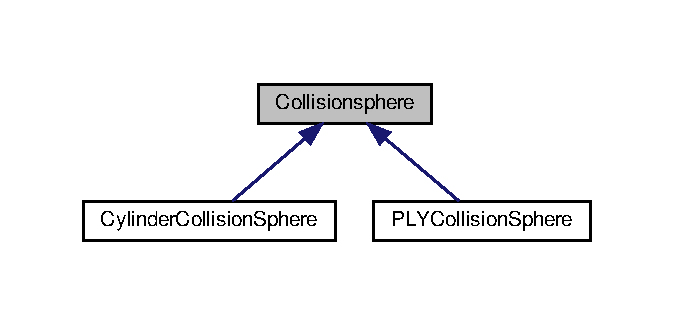
\includegraphics[width=324pt]{class_collisionsphere__inherit__graph}
\end{center}
\end{figure}
\subsection*{Public Attributes}
\begin{DoxyCompactItemize}
\item 
float \hyperlink{class_collisionsphere_a4b791781efcb1af5198b22ea0b542cfb}{big\+\_\+sphere\+\_\+distance}
\item 
float \hyperlink{class_collisionsphere_ae5430c092ea0436edfe0adeb79402ff2}{small\+\_\+sphere\+\_\+distance}
\item 
\mbox{\Hypertarget{class_collisionsphere_abf63a29c825cdd63ecb86d1dc430a0d4}\label{class_collisionsphere_abf63a29c825cdd63ecb86d1dc430a0d4}} 
unsigned {\bfseries list\+\_\+size}
\end{DoxyCompactItemize}


\subsection{Member Data Documentation}
\mbox{\Hypertarget{class_collisionsphere_a4b791781efcb1af5198b22ea0b542cfb}\label{class_collisionsphere_a4b791781efcb1af5198b22ea0b542cfb}} 
\index{Collisionsphere@{Collisionsphere}!big\+\_\+sphere\+\_\+distance@{big\+\_\+sphere\+\_\+distance}}
\index{big\+\_\+sphere\+\_\+distance@{big\+\_\+sphere\+\_\+distance}!Collisionsphere@{Collisionsphere}}
\subsubsection{\texorpdfstring{big\+\_\+sphere\+\_\+distance}{big\_sphere\_distance}}
{\footnotesize\ttfamily float Collisionsphere\+::big\+\_\+sphere\+\_\+distance}

Size of the big (outer) collision sphere \mbox{\Hypertarget{class_collisionsphere_ae5430c092ea0436edfe0adeb79402ff2}\label{class_collisionsphere_ae5430c092ea0436edfe0adeb79402ff2}} 
\index{Collisionsphere@{Collisionsphere}!small\+\_\+sphere\+\_\+distance@{small\+\_\+sphere\+\_\+distance}}
\index{small\+\_\+sphere\+\_\+distance@{small\+\_\+sphere\+\_\+distance}!Collisionsphere@{Collisionsphere}}
\subsubsection{\texorpdfstring{small\+\_\+sphere\+\_\+distance}{small\_sphere\_distance}}
{\footnotesize\ttfamily float Collisionsphere\+::small\+\_\+sphere\+\_\+distance}

Size of the small (inner) collision sphere 

The documentation for this class was generated from the following file\+:\begin{DoxyCompactItemize}
\item 
src/collisionsphere.\+h\end{DoxyCompactItemize}

\hypertarget{class_collisionspheren}{}\section{Collisionspheren Class Reference}
\label{class_collisionspheren}\index{Collisionspheren@{Collisionspheren}}


\hyperlink{class_collision}{Collision} Final class ============================================================================/.  




{\ttfamily \#include $<$collisionsphere.\+h$>$}



\subsection{Detailed Description}
\hyperlink{class_collision}{Collision} Final class ============================================================================/. 

Class to implement spherical bounding boxes for the W\+A\+L\+K\+ER mean diffusion. This class provides methods in order to create and update spherical bounding boxes used to compute the collisions. \begin{DoxyAuthor}{Author}
Jonathan Rafael \subsection*{February 2017 }
\end{DoxyAuthor}


Father class. this class provides methods in order to create and update spherical bounding box used to compute the collisions. The implementation is based on two collision spheres. The inner one (small) and the (outer). The fist saves the objects where th particle M\+AY collide in a given time, While the second saves the full set of obstacles where the particle can possibly collide, i.\+e. that are physically achievable for the walker to collide. 

The documentation for this class was generated from the following file\+:\begin{DoxyCompactItemize}
\item 
src/collisionsphere.\+h\end{DoxyCompactItemize}

\hypertarget{class_cylinder}{}\section{Cylinder Class Reference}
\label{class_cylinder}\index{Cylinder@{Cylinder}}


\hyperlink{class_cylinder}{Cylinder} \hyperlink{class_obstacle}{Obstacle} Derived Class =============================================================/.  




{\ttfamily \#include $<$cylinder.\+h$>$}



Inheritance diagram for Cylinder\+:
\nopagebreak
\begin{figure}[H]
\begin{center}
\leavevmode
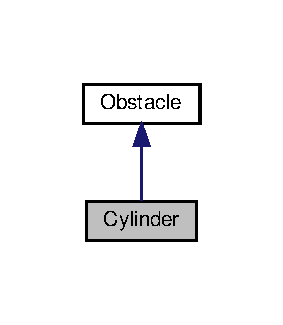
\includegraphics[width=136pt]{class_cylinder__inherit__graph}
\end{center}
\end{figure}


Collaboration diagram for Cylinder\+:
\nopagebreak
\begin{figure}[H]
\begin{center}
\leavevmode
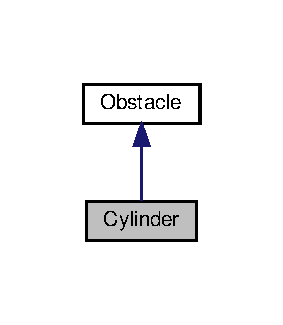
\includegraphics[width=136pt]{class_cylinder__coll__graph}
\end{center}
\end{figure}
\subsection*{Public Member Functions}
\begin{DoxyCompactItemize}
\item 
\mbox{\Hypertarget{class_cylinder_a01dc978cb576f834b9545e43d4dad2a2}\label{class_cylinder_a01dc978cb576f834b9545e43d4dad2a2}} 
\hyperlink{class_cylinder_a01dc978cb576f834b9545e43d4dad2a2}{Cylinder} ()
\begin{DoxyCompactList}\small\item\em Default constructor. Does nothing. \end{DoxyCompactList}\item 
\hyperlink{class_cylinder_a0a5f7aa0a0c5c5e17c783784fd99fa1a}{Cylinder} (Eigen\+::\+Vector3d P\+\_\+, Eigen\+::\+Vector3d Q\+\_\+, double radius\+\_\+, double scale=1)
\begin{DoxyCompactList}\small\item\em Initialize everything. \end{DoxyCompactList}\item 
\hyperlink{class_cylinder_ab5389301aa05bdee0c066e0b8026611f}{Cylinder} (\hyperlink{class_cylinder}{Cylinder} const \&cyl)
\begin{DoxyCompactList}\small\item\em Initialize everything. \end{DoxyCompactList}\item 
bool \hyperlink{class_cylinder_a43350a6331f8656dd0774a4a3b68724f}{check\+Collision} (\hyperlink{class_walker}{Walker} \&walker, Eigen\+::\+Vector3d \&step, double \&step\+\_\+lenght, \hyperlink{class_collision}{Collision} \&colision)
\begin{DoxyCompactList}\small\item\em Basic collision function. Returns the if there was any collision on against the obstacle. \end{DoxyCompactList}\item 
double \hyperlink{class_cylinder_a6eb639d12a7fc0aec50895151fb91b1f}{min\+Distance} (\hyperlink{class_walker}{Walker} \&w)
\begin{DoxyCompactList}\small\item\em Returns the minimum distance from the walker to the cylinder. Used to set the reachable cylinders that a given walker can reach. \end{DoxyCompactList}\end{DoxyCompactItemize}
\subsection*{Public Attributes}
\begin{DoxyCompactItemize}
\item 
\mbox{\Hypertarget{class_cylinder_ae9823df86b6b76bc86172d84d798494f}\label{class_cylinder_ae9823df86b6b76bc86172d84d798494f}} 
Eigen\+::\+Vector3d {\bfseries P}
\item 
Eigen\+::\+Vector3d \hyperlink{class_cylinder_a9f367beb008c847b97bb0ce043601769}{Q}
\item 
Eigen\+::\+Vector3d \hyperlink{class_cylinder_a2e7f0d4e406cc50daf30f3e3b0be1609}{D}
\item 
double \hyperlink{class_cylinder_a8a825799285bcf60b49b8aef0459b498}{radius}
\end{DoxyCompactItemize}
\subsection*{Static Public Attributes}
\begin{DoxyCompactItemize}
\item 
\mbox{\Hypertarget{class_cylinder_af276a253b655ded13f5dfd5afbff81d1}\label{class_cylinder_af276a253b655ded13f5dfd5afbff81d1}} 
static int {\bfseries count} = 0
\end{DoxyCompactItemize}


\subsection{Detailed Description}
\hyperlink{class_cylinder}{Cylinder} \hyperlink{class_obstacle}{Obstacle} Derived Class =============================================================/. 

\hyperlink{class_cylinder}{Cylinder} class derived from an \hyperlink{class_obstacle}{Obstacle}. Defines infinite long cylinders in the direction set by P,Q. \begin{DoxyAuthor}{Author}
Jonathan Rafael 
\end{DoxyAuthor}
\begin{DoxyDate}{Date}
November 2016 \subsection*{1.\+42 }
\end{DoxyDate}


\subsection{Constructor \& Destructor Documentation}
\mbox{\Hypertarget{class_cylinder_a0a5f7aa0a0c5c5e17c783784fd99fa1a}\label{class_cylinder_a0a5f7aa0a0c5c5e17c783784fd99fa1a}} 
\index{Cylinder@{Cylinder}!Cylinder@{Cylinder}}
\index{Cylinder@{Cylinder}!Cylinder@{Cylinder}}
\subsubsection{\texorpdfstring{Cylinder()}{Cylinder()}\hspace{0.1cm}{\footnotesize\ttfamily [1/2]}}
{\footnotesize\ttfamily Cylinder\+::\+Cylinder (\begin{DoxyParamCaption}\item[{Eigen\+::\+Vector3d}]{P\+\_\+,  }\item[{Eigen\+::\+Vector3d}]{Q\+\_\+,  }\item[{double}]{radius\+\_\+,  }\item[{double}]{scale = {\ttfamily 1} }\end{DoxyParamCaption})\hspace{0.3cm}{\ttfamily [inline]}}



Initialize everything. 


\begin{DoxyParams}{Parameters}
{\em P\+\_\+} & \hyperlink{class_cylinder}{Cylinder} origin \\
\hline
{\em Q\+\_\+} & cylinder direction. \\
\hline
{\em radius\+\_\+} & cylinder\textquotesingle{}s radius \\
\hline
{\em scale} & scale factor for the values passed. Useful when reading a file. \\
\hline
\end{DoxyParams}
\mbox{\Hypertarget{class_cylinder_ab5389301aa05bdee0c066e0b8026611f}\label{class_cylinder_ab5389301aa05bdee0c066e0b8026611f}} 
\index{Cylinder@{Cylinder}!Cylinder@{Cylinder}}
\index{Cylinder@{Cylinder}!Cylinder@{Cylinder}}
\subsubsection{\texorpdfstring{Cylinder()}{Cylinder()}\hspace{0.1cm}{\footnotesize\ttfamily [2/2]}}
{\footnotesize\ttfamily Cylinder\+::\+Cylinder (\begin{DoxyParamCaption}\item[{\hyperlink{class_cylinder}{Cylinder} const \&}]{cyl }\end{DoxyParamCaption})}



Initialize everything. 


\begin{DoxyParams}{Parameters}
{\em P\+\_\+} & \hyperlink{class_cylinder}{Cylinder} origin \\
\hline
{\em Q\+\_\+} & cylinder direction. \\
\hline
{\em radius\+\_\+} & cylinder\textquotesingle{}s radius \\
\hline
{\em scale} & scale factor for the values passed. Useful when reading a file. \\
\hline
\end{DoxyParams}


\subsection{Member Function Documentation}
\mbox{\Hypertarget{class_cylinder_a43350a6331f8656dd0774a4a3b68724f}\label{class_cylinder_a43350a6331f8656dd0774a4a3b68724f}} 
\index{Cylinder@{Cylinder}!check\+Collision@{check\+Collision}}
\index{check\+Collision@{check\+Collision}!Cylinder@{Cylinder}}
\subsubsection{\texorpdfstring{check\+Collision()}{checkCollision()}}
{\footnotesize\ttfamily Cylinder\+::check\+Collision (\begin{DoxyParamCaption}\item[{\hyperlink{class_walker}{Walker} \&}]{walker,  }\item[{Eigen\+::\+Vector3d \&}]{step,  }\item[{double \&}]{step\+\_\+lenght,  }\item[{\hyperlink{class_collision}{Collision} \&}]{colision }\end{DoxyParamCaption})}



Basic collision function. Returns the if there was any collision on against the obstacle. 


\begin{DoxyParams}{Parameters}
{\em walker,\hyperlink{class_walker}{Walker}} & instance in the simulation. \\
\hline
{\em 3d} & step. Is assumed to be normalized. \\
\hline
{\em step\+\_\+length,length} & used as the maximum step collision distance. \\
\hline
{\em collision,\hyperlink{class_collision}{Collision}} & instance to save the collision (if any) details. \\
\hline
\end{DoxyParams}
\begin{DoxyReturn}{Returns}
true only if there was a Collision\+::hit status. 
\end{DoxyReturn}
\begin{DoxySeeAlso}{See also}
\hyperlink{class_collision}{Collision}. 
\end{DoxySeeAlso}
\mbox{\Hypertarget{class_cylinder_a6eb639d12a7fc0aec50895151fb91b1f}\label{class_cylinder_a6eb639d12a7fc0aec50895151fb91b1f}} 
\index{Cylinder@{Cylinder}!min\+Distance@{min\+Distance}}
\index{min\+Distance@{min\+Distance}!Cylinder@{Cylinder}}
\subsubsection{\texorpdfstring{min\+Distance()}{minDistance()}}
{\footnotesize\ttfamily Cylinder\+::min\+Distance (\begin{DoxyParamCaption}\item[{\hyperlink{class_walker}{Walker} \&}]{w }\end{DoxyParamCaption})}



Returns the minimum distance from the walker to the cylinder. Used to set the reachable cylinders that a given walker can reach. 


\begin{DoxyParams}{Parameters}
{\em walker,\hyperlink{class_walker}{Walker}} & instance in the simulation. \\
\hline
\end{DoxyParams}


\subsection{Member Data Documentation}
\mbox{\Hypertarget{class_cylinder_a2e7f0d4e406cc50daf30f3e3b0be1609}\label{class_cylinder_a2e7f0d4e406cc50daf30f3e3b0be1609}} 
\index{Cylinder@{Cylinder}!D@{D}}
\index{D@{D}!Cylinder@{Cylinder}}
\subsubsection{\texorpdfstring{D}{D}}
{\footnotesize\ttfamily Eigen\+::\+Vector3d Cylinder\+::D}

Pre-\/computed and normalized P -\/ Q vector \mbox{\Hypertarget{class_cylinder_a9f367beb008c847b97bb0ce043601769}\label{class_cylinder_a9f367beb008c847b97bb0ce043601769}} 
\index{Cylinder@{Cylinder}!Q@{Q}}
\index{Q@{Q}!Cylinder@{Cylinder}}
\subsubsection{\texorpdfstring{Q}{Q}}
{\footnotesize\ttfamily Eigen\+::\+Vector3d Cylinder\+::Q}

Cilinder Axis reference Points, P should be the \char`\"{}center\char`\"{} \mbox{\Hypertarget{class_cylinder_a8a825799285bcf60b49b8aef0459b498}\label{class_cylinder_a8a825799285bcf60b49b8aef0459b498}} 
\index{Cylinder@{Cylinder}!radius@{radius}}
\index{radius@{radius}!Cylinder@{Cylinder}}
\subsubsection{\texorpdfstring{radius}{radius}}
{\footnotesize\ttfamily double Cylinder\+::radius}

Radius of the cylinder 

The documentation for this class was generated from the following files\+:\begin{DoxyCompactItemize}
\item 
src/cylinder.\+h\item 
src/cylinder.\+cpp\end{DoxyCompactItemize}

\hypertarget{class_cylinder_collision_sphere}{}\section{Cylinder\+Collision\+Sphere Class Reference}
\label{class_cylinder_collision_sphere}\index{Cylinder\+Collision\+Sphere@{Cylinder\+Collision\+Sphere}}


Class to save the cylinderical obstacles that a can collide to a walker.  




{\ttfamily \#include $<$collisionsphere.\+h$>$}



Inheritance diagram for Cylinder\+Collision\+Sphere\+:\nopagebreak
\begin{figure}[H]
\begin{center}
\leavevmode
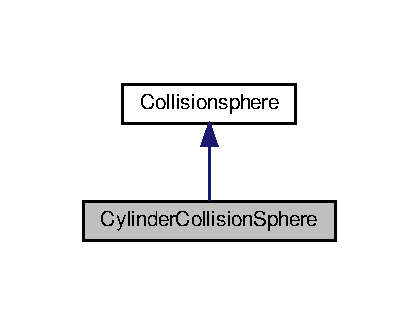
\includegraphics[width=201pt]{class_cylinder_collision_sphere__inherit__graph}
\end{center}
\end{figure}


Collaboration diagram for Cylinder\+Collision\+Sphere\+:\nopagebreak
\begin{figure}[H]
\begin{center}
\leavevmode
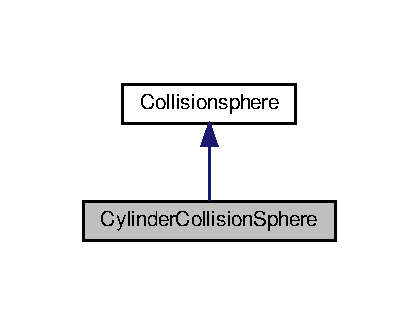
\includegraphics[width=201pt]{class_cylinder_collision_sphere__coll__graph}
\end{center}
\end{figure}
\subsection*{Public Member Functions}
\begin{DoxyCompactItemize}
\item 
\hyperlink{class_cylinder_collision_sphere_ac4f58e8792fdcdfe475b9556dc804553}{Cylinder\+Collision\+Sphere} ()
\item 
\mbox{\Hypertarget{class_cylinder_collision_sphere_ad4cfd86c6ab7035b9ba67277792c132f}\label{class_cylinder_collision_sphere_ad4cfd86c6ab7035b9ba67277792c132f}} 
void \hyperlink{class_cylinder_collision_sphere_ad4cfd86c6ab7035b9ba67277792c132f}{pop\+From\+Small\+Sphere} (unsigned i)
\begin{DoxyCompactList}\small\item\em This function receives a index from the collision list and moves the value to the last position of the list. then decrease the inner sphere end index. This way this index is no longer considered inner collision list. \end{DoxyCompactList}\item 
\mbox{\Hypertarget{class_cylinder_collision_sphere_aa369aaa1ce839382c915ac4f32ac82ca}\label{class_cylinder_collision_sphere_aa369aaa1ce839382c915ac4f32ac82ca}} 
void \hyperlink{class_cylinder_collision_sphere_aa369aaa1ce839382c915ac4f32ac82ca}{push\+To\+Small\+Sphere} (unsigned i)
\begin{DoxyCompactList}\small\item\em This function receives a index from the collision list and moves the value to the last position of the list. then increase the inner sphere end index. This way this index is now included in the inner collision list. \end{DoxyCompactList}\item 
\mbox{\Hypertarget{class_cylinder_collision_sphere_a06a8f75674ef0bcc44a820e948624f60}\label{class_cylinder_collision_sphere_a06a8f75674ef0bcc44a820e948624f60}} 
void \hyperlink{class_cylinder_collision_sphere_a06a8f75674ef0bcc44a820e948624f60}{pop\+From\+Big\+Sphere} (unsigned i)
\begin{DoxyCompactList}\small\item\em This function receives a index from the collision list and moves the value to the last position of the list. Then decrease the inner sphere end index. This way this index is now excluded in the outer collision list. \end{DoxyCompactList}\item 
\mbox{\Hypertarget{class_cylinder_collision_sphere_a8742564f85c9fede195ee716a3b16042}\label{class_cylinder_collision_sphere_a8742564f85c9fede195ee716a3b16042}} 
void \hyperlink{class_cylinder_collision_sphere_a8742564f85c9fede195ee716a3b16042}{push\+To\+Big\+Sphere} (unsigned i)
\begin{DoxyCompactList}\small\item\em This function receives a index from the collision list and moves the value to the last position of the list. Then increase the inner sphere end index. This way this index is now included in the outer collision list. \end{DoxyCompactList}\item 
void \hyperlink{class_cylinder_collision_sphere_a3fe165c817a66074e737985efd87128b}{set\+Big\+Sphere\+Size} (float size)
\item 
void \hyperlink{class_cylinder_collision_sphere_a6e7f5ff8f4e5c076edb5f1cbee433a34}{set\+Small\+Sphere\+Size} (float size)
\item 
void \hyperlink{class_cylinder_collision_sphere_af2977e3da60e7a4c1e4ae4fccf03ed09}{push\+\_\+index} (unsigned int element)
\end{DoxyCompactItemize}
\subsection*{Public Attributes}
\begin{DoxyCompactItemize}
\item 
unsigned \hyperlink{class_cylinder_collision_sphere_a89e3bdfa12042aa94c20949587c513d5}{small\+\_\+sphere\+\_\+list\+\_\+end}
\item 
unsigned \hyperlink{class_cylinder_collision_sphere_a303b3843a9c8ab9ae3e6f4cce85ae8e0}{big\+\_\+sphere\+\_\+list\+\_\+end}
\item 
\mbox{\Hypertarget{class_cylinder_collision_sphere_a2c925c436410847d2f6079cd5331eada}\label{class_cylinder_collision_sphere_a2c925c436410847d2f6079cd5331eada}} 
std\+::vector$<$ unsigned $>$ $\ast$ {\bfseries collision\+\_\+list}
\end{DoxyCompactItemize}


\subsection{Detailed Description}
Class to save the cylinderical obstacles that a can collide to a walker. 

Class to save the P\+LY mehses and the subset of triangles that a can collide to a walker. 

\subsection{Constructor \& Destructor Documentation}
\mbox{\Hypertarget{class_cylinder_collision_sphere_ac4f58e8792fdcdfe475b9556dc804553}\label{class_cylinder_collision_sphere_ac4f58e8792fdcdfe475b9556dc804553}} 
\index{Cylinder\+Collision\+Sphere@{Cylinder\+Collision\+Sphere}!Cylinder\+Collision\+Sphere@{Cylinder\+Collision\+Sphere}}
\index{Cylinder\+Collision\+Sphere@{Cylinder\+Collision\+Sphere}!Cylinder\+Collision\+Sphere@{Cylinder\+Collision\+Sphere}}
\subsubsection{\texorpdfstring{Cylinder\+Collision\+Sphere()}{CylinderCollisionSphere()}}
{\footnotesize\ttfamily Cylinder\+Collision\+Sphere\+::\+Cylinder\+Collision\+Sphere (\begin{DoxyParamCaption}{ }\end{DoxyParamCaption})}

$<$Pointer to List with the cylinders indexes. The indexes are permuted in its position. 

\subsection{Member Function Documentation}
\mbox{\Hypertarget{class_cylinder_collision_sphere_af2977e3da60e7a4c1e4ae4fccf03ed09}\label{class_cylinder_collision_sphere_af2977e3da60e7a4c1e4ae4fccf03ed09}} 
\index{Cylinder\+Collision\+Sphere@{Cylinder\+Collision\+Sphere}!push\+\_\+index@{push\+\_\+index}}
\index{push\+\_\+index@{push\+\_\+index}!Cylinder\+Collision\+Sphere@{Cylinder\+Collision\+Sphere}}
\subsubsection{\texorpdfstring{push\+\_\+index()}{push\_index()}}
{\footnotesize\ttfamily void Cylinder\+Collision\+Sphere\+::push\+\_\+index (\begin{DoxyParamCaption}\item[{unsigned int}]{element }\end{DoxyParamCaption})}


\begin{DoxyParams}{Parameters}
{\em element} & value to be added to the obstacle list \\
\hline
\end{DoxyParams}
\mbox{\Hypertarget{class_cylinder_collision_sphere_a3fe165c817a66074e737985efd87128b}\label{class_cylinder_collision_sphere_a3fe165c817a66074e737985efd87128b}} 
\index{Cylinder\+Collision\+Sphere@{Cylinder\+Collision\+Sphere}!set\+Big\+Sphere\+Size@{set\+Big\+Sphere\+Size}}
\index{set\+Big\+Sphere\+Size@{set\+Big\+Sphere\+Size}!Cylinder\+Collision\+Sphere@{Cylinder\+Collision\+Sphere}}
\subsubsection{\texorpdfstring{set\+Big\+Sphere\+Size()}{setBigSphereSize()}}
{\footnotesize\ttfamily void Cylinder\+Collision\+Sphere\+::set\+Big\+Sphere\+Size (\begin{DoxyParamCaption}\item[{float}]{size }\end{DoxyParamCaption})}


\begin{DoxyParams}{Parameters}
{\em size} & of the list \\
\hline
\end{DoxyParams}
\mbox{\Hypertarget{class_cylinder_collision_sphere_a6e7f5ff8f4e5c076edb5f1cbee433a34}\label{class_cylinder_collision_sphere_a6e7f5ff8f4e5c076edb5f1cbee433a34}} 
\index{Cylinder\+Collision\+Sphere@{Cylinder\+Collision\+Sphere}!set\+Small\+Sphere\+Size@{set\+Small\+Sphere\+Size}}
\index{set\+Small\+Sphere\+Size@{set\+Small\+Sphere\+Size}!Cylinder\+Collision\+Sphere@{Cylinder\+Collision\+Sphere}}
\subsubsection{\texorpdfstring{set\+Small\+Sphere\+Size()}{setSmallSphereSize()}}
{\footnotesize\ttfamily void Cylinder\+Collision\+Sphere\+::set\+Small\+Sphere\+Size (\begin{DoxyParamCaption}\item[{float}]{size }\end{DoxyParamCaption})}


\begin{DoxyParams}{Parameters}
{\em size} & of the list \\
\hline
\end{DoxyParams}


\subsection{Member Data Documentation}
\mbox{\Hypertarget{class_cylinder_collision_sphere_a303b3843a9c8ab9ae3e6f4cce85ae8e0}\label{class_cylinder_collision_sphere_a303b3843a9c8ab9ae3e6f4cce85ae8e0}} 
\index{Cylinder\+Collision\+Sphere@{Cylinder\+Collision\+Sphere}!big\+\_\+sphere\+\_\+list\+\_\+end@{big\+\_\+sphere\+\_\+list\+\_\+end}}
\index{big\+\_\+sphere\+\_\+list\+\_\+end@{big\+\_\+sphere\+\_\+list\+\_\+end}!Cylinder\+Collision\+Sphere@{Cylinder\+Collision\+Sphere}}
\subsubsection{\texorpdfstring{big\+\_\+sphere\+\_\+list\+\_\+end}{big\_sphere\_list\_end}}
{\footnotesize\ttfamily unsigned Cylinder\+Collision\+Sphere\+::big\+\_\+sphere\+\_\+list\+\_\+end}

Index of the L\+A\+ST element on the list for the big collision sphere \mbox{\Hypertarget{class_cylinder_collision_sphere_a89e3bdfa12042aa94c20949587c513d5}\label{class_cylinder_collision_sphere_a89e3bdfa12042aa94c20949587c513d5}} 
\index{Cylinder\+Collision\+Sphere@{Cylinder\+Collision\+Sphere}!small\+\_\+sphere\+\_\+list\+\_\+end@{small\+\_\+sphere\+\_\+list\+\_\+end}}
\index{small\+\_\+sphere\+\_\+list\+\_\+end@{small\+\_\+sphere\+\_\+list\+\_\+end}!Cylinder\+Collision\+Sphere@{Cylinder\+Collision\+Sphere}}
\subsubsection{\texorpdfstring{small\+\_\+sphere\+\_\+list\+\_\+end}{small\_sphere\_list\_end}}
{\footnotesize\ttfamily unsigned Cylinder\+Collision\+Sphere\+::small\+\_\+sphere\+\_\+list\+\_\+end}

Index of the L\+A\+ST element on the list for the small collision sphere 

The documentation for this class was generated from the following files\+:\begin{DoxyCompactItemize}
\item 
src/collisionsphere.\+h\item 
src/collisionsphere.\+cpp\end{DoxyCompactItemize}

\hypertarget{class_cylinder_gamma_distribution}{}\section{Cylinder\+Gamma\+Distribution Class Reference}
\label{class_cylinder_gamma_distribution}\index{Cylinder\+Gamma\+Distribution@{Cylinder\+Gamma\+Distribution}}


\hyperlink{class_cylinder_gamma_distribution}{Cylinder\+Gamma\+Distribution} Class =============================================================/.  




{\ttfamily \#include $<$cylindergammadistribution.\+h$>$}

\subsection*{Public Member Functions}
\begin{DoxyCompactItemize}
\item 
\hyperlink{class_cylinder_gamma_distribution_a7578f5f0fb11398ec5bf5007047f4b81}{Cylinder\+Gamma\+Distribution} (unsigned, double, double, double, Eigen\+::\+Vector3d \&, Eigen\+::\+Vector3d \&, float \hyperlink{class_cylinder_gamma_distribution_aece7d3ec40d3dbb3a2ecd1bd88c5a694}{min\+\_\+radius})
\begin{DoxyCompactList}\small\item\em Initialize everything. \end{DoxyCompactList}\item 
\mbox{\Hypertarget{class_cylinder_gamma_distribution_a3408ed30966550c10810a0a6cbbfd3c2}\label{class_cylinder_gamma_distribution_a3408ed30966550c10810a0a6cbbfd3c2}} 
void \hyperlink{class_cylinder_gamma_distribution_a3408ed30966550c10810a0a6cbbfd3c2}{display\+Gamma\+Distribution} ()
\begin{DoxyCompactList}\small\item\em Shows a small histogram of the gamma distribution. \end{DoxyCompactList}\item 
\mbox{\Hypertarget{class_cylinder_gamma_distribution_ad93e569b24e3c6b1266ecf79bd18dec9}\label{class_cylinder_gamma_distribution_ad93e569b24e3c6b1266ecf79bd18dec9}} 
void \hyperlink{class_cylinder_gamma_distribution_ad93e569b24e3c6b1266ecf79bd18dec9}{create\+Gamma\+Substrate} ()
\begin{DoxyCompactList}\small\item\em Samples and constructs a Gamma distribution. \end{DoxyCompactList}\item 
void \hyperlink{class_cylinder_gamma_distribution_a2345c03be0b0c934efe02e4234c65fd1}{print\+Substrate} (std\+::ostream \&out)
\begin{DoxyCompactList}\small\item\em Prints the cylinders positions in a file or output stream. \end{DoxyCompactList}\end{DoxyCompactItemize}
\subsection*{Public Attributes}
\begin{DoxyCompactItemize}
\item 
unsigned \hyperlink{class_cylinder_gamma_distribution_af74583662a4f33ba1565f2c71e6bbc5a}{num\+\_\+cylinders}
\item 
double \hyperlink{class_cylinder_gamma_distribution_a8cae528f51692ed05049e4ea06c63722}{alpha}
\item 
double \hyperlink{class_cylinder_gamma_distribution_a601a42ef7bacbf9696229efbd703f61e}{beta}
\item 
double \hyperlink{class_cylinder_gamma_distribution_a31f82c4608b7cd2b022805e30a4db983}{icvf}
\item 
float \hyperlink{class_cylinder_gamma_distribution_aece7d3ec40d3dbb3a2ecd1bd88c5a694}{min\+\_\+radius}
\item 
Eigen\+::\+Vector3d \hyperlink{class_cylinder_gamma_distribution_ac77a9d794f2f2000066c4a26f19a9097}{min\+\_\+limits}
\item 
Eigen\+::\+Vector3d \hyperlink{class_cylinder_gamma_distribution_aa7094851c2ccf05fc5ff7a99707aa786}{max\+\_\+limits}
\item 
std\+::vector$<$ \hyperlink{class_cylinder}{Cylinder} $>$ \hyperlink{class_cylinder_gamma_distribution_a3e8265a7ddb15d895112e02bd66fbf67}{cylinders}
\end{DoxyCompactItemize}


\subsection{Detailed Description}
\hyperlink{class_cylinder_gamma_distribution}{Cylinder\+Gamma\+Distribution} Class =============================================================/. 

Class to construct a substrate taken from a Gamma distribution of radiis placed in a single voxel structure. \begin{DoxyAuthor}{Author}
Jonathan Rafael 
\end{DoxyAuthor}
\begin{DoxyDate}{Date}
february 2017 \subsection*{0.\+2 }
\end{DoxyDate}


\subsection{Constructor \& Destructor Documentation}
\mbox{\Hypertarget{class_cylinder_gamma_distribution_a7578f5f0fb11398ec5bf5007047f4b81}\label{class_cylinder_gamma_distribution_a7578f5f0fb11398ec5bf5007047f4b81}} 
\index{Cylinder\+Gamma\+Distribution@{Cylinder\+Gamma\+Distribution}!Cylinder\+Gamma\+Distribution@{Cylinder\+Gamma\+Distribution}}
\index{Cylinder\+Gamma\+Distribution@{Cylinder\+Gamma\+Distribution}!Cylinder\+Gamma\+Distribution@{Cylinder\+Gamma\+Distribution}}
\subsubsection{\texorpdfstring{Cylinder\+Gamma\+Distribution()}{CylinderGammaDistribution()}}
{\footnotesize\ttfamily Cylinder\+Gamma\+Distribution\+::\+Cylinder\+Gamma\+Distribution (\begin{DoxyParamCaption}\item[{unsigned}]{num\+\_\+cyl,  }\item[{double}]{a,  }\item[{double}]{b,  }\item[{double}]{icvf\+\_\+,  }\item[{Eigen\+::\+Vector3d \&}]{min\+\_\+l,  }\item[{Eigen\+::\+Vector3d \&}]{max\+\_\+l,  }\item[{float}]{min\+\_\+radius = {\ttfamily 0.01} }\end{DoxyParamCaption})}



Initialize everything. 


\begin{DoxyParams}{Parameters}
{\em P\+\_\+} & \hyperlink{class_cylinder}{Cylinder} origin \\
\hline
{\em Q\+\_\+} & cylinder direction. \\
\hline
{\em radius\+\_\+} & cylinder\textquotesingle{}s radius \\
\hline
{\em scale} & scale factor for the values passed. Useful when reading a file. \\
\hline
\end{DoxyParams}


\subsection{Member Function Documentation}
\mbox{\Hypertarget{class_cylinder_gamma_distribution_a2345c03be0b0c934efe02e4234c65fd1}\label{class_cylinder_gamma_distribution_a2345c03be0b0c934efe02e4234c65fd1}} 
\index{Cylinder\+Gamma\+Distribution@{Cylinder\+Gamma\+Distribution}!print\+Substrate@{print\+Substrate}}
\index{print\+Substrate@{print\+Substrate}!Cylinder\+Gamma\+Distribution@{Cylinder\+Gamma\+Distribution}}
\subsubsection{\texorpdfstring{print\+Substrate()}{printSubstrate()}}
{\footnotesize\ttfamily void Cylinder\+Gamma\+Distribution\+::print\+Substrate (\begin{DoxyParamCaption}\item[{std\+::ostream \&}]{out }\end{DoxyParamCaption})}



Prints the cylinders positions in a file or output stream. 


\begin{DoxyParams}{Parameters}
{\em out} & ostream where to write the info. \\
\hline
\end{DoxyParams}


\subsection{Member Data Documentation}
\mbox{\Hypertarget{class_cylinder_gamma_distribution_a8cae528f51692ed05049e4ea06c63722}\label{class_cylinder_gamma_distribution_a8cae528f51692ed05049e4ea06c63722}} 
\index{Cylinder\+Gamma\+Distribution@{Cylinder\+Gamma\+Distribution}!alpha@{alpha}}
\index{alpha@{alpha}!Cylinder\+Gamma\+Distribution@{Cylinder\+Gamma\+Distribution}}
\subsubsection{\texorpdfstring{alpha}{alpha}}
{\footnotesize\ttfamily double Cylinder\+Gamma\+Distribution\+::alpha}

alpha coefficient of the Gamma distribution \mbox{\Hypertarget{class_cylinder_gamma_distribution_a601a42ef7bacbf9696229efbd703f61e}\label{class_cylinder_gamma_distribution_a601a42ef7bacbf9696229efbd703f61e}} 
\index{Cylinder\+Gamma\+Distribution@{Cylinder\+Gamma\+Distribution}!beta@{beta}}
\index{beta@{beta}!Cylinder\+Gamma\+Distribution@{Cylinder\+Gamma\+Distribution}}
\subsubsection{\texorpdfstring{beta}{beta}}
{\footnotesize\ttfamily double Cylinder\+Gamma\+Distribution\+::beta}

beta coefficient of the gamma distribution \mbox{\Hypertarget{class_cylinder_gamma_distribution_a3e8265a7ddb15d895112e02bd66fbf67}\label{class_cylinder_gamma_distribution_a3e8265a7ddb15d895112e02bd66fbf67}} 
\index{Cylinder\+Gamma\+Distribution@{Cylinder\+Gamma\+Distribution}!cylinders@{cylinders}}
\index{cylinders@{cylinders}!Cylinder\+Gamma\+Distribution@{Cylinder\+Gamma\+Distribution}}
\subsubsection{\texorpdfstring{cylinders}{cylinders}}
{\footnotesize\ttfamily std\+::vector$<$\hyperlink{class_cylinder}{Cylinder}$>$ Cylinder\+Gamma\+Distribution\+::cylinders}

\hyperlink{class_cylinder}{Cylinder} vector \mbox{\Hypertarget{class_cylinder_gamma_distribution_a31f82c4608b7cd2b022805e30a4db983}\label{class_cylinder_gamma_distribution_a31f82c4608b7cd2b022805e30a4db983}} 
\index{Cylinder\+Gamma\+Distribution@{Cylinder\+Gamma\+Distribution}!icvf@{icvf}}
\index{icvf@{icvf}!Cylinder\+Gamma\+Distribution@{Cylinder\+Gamma\+Distribution}}
\subsubsection{\texorpdfstring{icvf}{icvf}}
{\footnotesize\ttfamily double Cylinder\+Gamma\+Distribution\+::icvf}

Achieved intra-\/celular volum fraction in the substrate \mbox{\Hypertarget{class_cylinder_gamma_distribution_aa7094851c2ccf05fc5ff7a99707aa786}\label{class_cylinder_gamma_distribution_aa7094851c2ccf05fc5ff7a99707aa786}} 
\index{Cylinder\+Gamma\+Distribution@{Cylinder\+Gamma\+Distribution}!max\+\_\+limits@{max\+\_\+limits}}
\index{max\+\_\+limits@{max\+\_\+limits}!Cylinder\+Gamma\+Distribution@{Cylinder\+Gamma\+Distribution}}
\subsubsection{\texorpdfstring{max\+\_\+limits}{max\_limits}}
{\footnotesize\ttfamily Eigen\+::\+Vector3d Cylinder\+Gamma\+Distribution\+::max\+\_\+limits}

voxel max limits (if any) \mbox{\Hypertarget{class_cylinder_gamma_distribution_ac77a9d794f2f2000066c4a26f19a9097}\label{class_cylinder_gamma_distribution_ac77a9d794f2f2000066c4a26f19a9097}} 
\index{Cylinder\+Gamma\+Distribution@{Cylinder\+Gamma\+Distribution}!min\+\_\+limits@{min\+\_\+limits}}
\index{min\+\_\+limits@{min\+\_\+limits}!Cylinder\+Gamma\+Distribution@{Cylinder\+Gamma\+Distribution}}
\subsubsection{\texorpdfstring{min\+\_\+limits}{min\_limits}}
{\footnotesize\ttfamily Eigen\+::\+Vector3d Cylinder\+Gamma\+Distribution\+::min\+\_\+limits}

voxel min limits (if any) (bottom left corner) \mbox{\Hypertarget{class_cylinder_gamma_distribution_aece7d3ec40d3dbb3a2ecd1bd88c5a694}\label{class_cylinder_gamma_distribution_aece7d3ec40d3dbb3a2ecd1bd88c5a694}} 
\index{Cylinder\+Gamma\+Distribution@{Cylinder\+Gamma\+Distribution}!min\+\_\+radius@{min\+\_\+radius}}
\index{min\+\_\+radius@{min\+\_\+radius}!Cylinder\+Gamma\+Distribution@{Cylinder\+Gamma\+Distribution}}
\subsubsection{\texorpdfstring{min\+\_\+radius}{min\_radius}}
{\footnotesize\ttfamily float Cylinder\+Gamma\+Distribution\+::min\+\_\+radius}

Minimum radius to be sampled from the gamma distribution \mbox{\Hypertarget{class_cylinder_gamma_distribution_af74583662a4f33ba1565f2c71e6bbc5a}\label{class_cylinder_gamma_distribution_af74583662a4f33ba1565f2c71e6bbc5a}} 
\index{Cylinder\+Gamma\+Distribution@{Cylinder\+Gamma\+Distribution}!num\+\_\+cylinders@{num\+\_\+cylinders}}
\index{num\+\_\+cylinders@{num\+\_\+cylinders}!Cylinder\+Gamma\+Distribution@{Cylinder\+Gamma\+Distribution}}
\subsubsection{\texorpdfstring{num\+\_\+cylinders}{num\_cylinders}}
{\footnotesize\ttfamily unsigned Cylinder\+Gamma\+Distribution\+::num\+\_\+cylinders}

number of cylnders fit inside the substrate 

The documentation for this class was generated from the following files\+:\begin{DoxyCompactItemize}
\item 
src/cylindergammadistribution.\+h\item 
src/cylindergammadistribution.\+cpp\end{DoxyCompactItemize}

\hypertarget{class_dynamics_simulation}{}\section{Dynamics\+Simulation Class Reference}
\label{class_dynamics_simulation}\index{Dynamics\+Simulation@{Dynamics\+Simulation}}


Dynamic simulation main class =============================================================/.  




{\ttfamily \#include $<$dynamics\+Simulation.\+h$>$}



Collaboration diagram for Dynamics\+Simulation\+:
\nopagebreak
\begin{figure}[H]
\begin{center}
\leavevmode
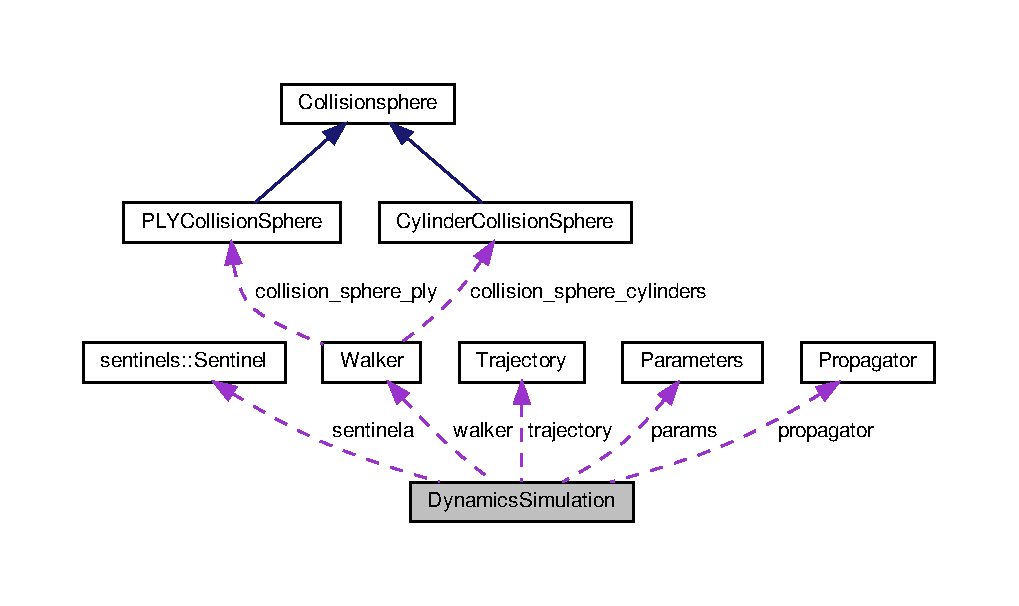
\includegraphics[width=350pt]{class_dynamics_simulation__coll__graph}
\end{center}
\end{figure}
\subsection*{Public Member Functions}
\begin{DoxyCompactItemize}
\item 
\hyperlink{class_dynamics_simulation_ad9a3e1f235466c3827cb49c67d3a6147}{Dynamics\+Simulation} ()
\begin{DoxyCompactList}\small\item\em Default constructor. Initialize everything with 0\textquotesingle{}s and N\+U\+LL states, object indexes are set to -\/1. \end{DoxyCompactList}\item 
\hyperlink{class_dynamics_simulation_aa603b5ba682b1b37cc96dd8be113cb52}{Dynamics\+Simulation} (std\+::string conf\+\_\+file)
\item 
\hyperlink{class_dynamics_simulation_a8fd2ec6f3640bff79e4b1ad960bbda5b}{Dynamics\+Simulation} (\hyperlink{class_parameters}{Parameters} \&params\+\_\+)
\item 
\mbox{\Hypertarget{class_dynamics_simulation_a15a1f18a99d606ef2ca939e718ca996f}\label{class_dynamics_simulation_a15a1f18a99d606ef2ca939e718ca996f}} 
\hyperlink{class_dynamics_simulation_a15a1f18a99d606ef2ca939e718ca996f}{$\sim$\+Dynamics\+Simulation} ()
\begin{DoxyCompactList}\small\item\em Does nothing. \end{DoxyCompactList}\item 
void \hyperlink{class_dynamics_simulation_a00cf4a6cbde1ef708fdbd58e8d8a7727}{start\+Simulation} (\hyperlink{class_simulable_sequence}{Simulable\+Sequence} $\ast$data\+Synth=nullptr)
\begin{DoxyCompactList}\small\item\em Starts the dynamics simulation and, if a P\+G\+SE sequence is given, computes the DW signal. \end{DoxyCompactList}\item 
void \hyperlink{class_dynamics_simulation_a67adab75eba635447c1b1b2b26d1e0ab}{read\+Configuration\+File} (std\+::string conf\+\_\+file\+\_\+path)
\begin{DoxyCompactList}\small\item\em Reads all the parameters listed in the param conf\+\_\+file and stores them in the /t params object. \end{DoxyCompactList}\item 
void \hyperlink{class_dynamics_simulation_a9148a30590bef5c766fd2366bbd16eb8}{set\+Duration} (const double \&duration)
\begin{DoxyCompactList}\small\item\em Sets the simulation duration in milliseconds, this should be synchronized w/r the Time Echo. \end{DoxyCompactList}\item 
\mbox{\Hypertarget{class_dynamics_simulation_a25b78b4ef659a448a806b995a19cf8b1}\label{class_dynamics_simulation_a25b78b4ef659a448a806b995a19cf8b1}} 
void {\bfseries set\+Walkers\+Num} (const unsigned \&N)
\item 
\mbox{\Hypertarget{class_dynamics_simulation_a45248ef6170eaf8a3a62b43f3ce77e02}\label{class_dynamics_simulation_a45248ef6170eaf8a3a62b43f3ce77e02}} 
void {\bfseries set\+Steps\+Num} (const unsigned \&T)
\item 
bool \hyperlink{class_dynamics_simulation_ae7aa76c335aceb658a4ffc683898077c}{is\+In\+Intra} (Eigen\+::\+Vector3d \&position, int \&cyl\+\_\+id, int \&ply\+\_\+id, double distance\+\_\+to\+\_\+be\+\_\+intra\+\_\+ply=1e-\/6)
\begin{DoxyCompactList}\small\item\em return true if the position is inside any of the obstacles. Only obstacles with a defined \char`\"{}inside region\char`\"{} can be considered. \hyperlink{class_voxel}{Voxel} periodicity is not considered \end{DoxyCompactList}\item 
\mbox{\Hypertarget{class_dynamics_simulation_aeae993217cebb5c23f68cb3e04cf8e49}\label{class_dynamics_simulation_aeae993217cebb5c23f68cb3e04cf8e49}} 
void \hyperlink{class_dynamics_simulation_aeae993217cebb5c23f68cb3e04cf8e49}{write\+Propagator} (std\+::string path)
\begin{DoxyCompactList}\small\item\em Writes to disk the final propagator matrix. \end{DoxyCompactList}\item 
\mbox{\Hypertarget{class_dynamics_simulation_a6c69cd2599f088e7631be0721d5815f1}\label{class_dynamics_simulation_a6c69cd2599f088e7631be0721d5815f1}} 
bool {\bfseries is\+Inside\+Cylinders} (Eigen\+::\+Vector3d \&position, int \&cyl\+\_\+id, double distance\+\_\+to\+\_\+be\+\_\+inside=1e-\/6)
\item 
\mbox{\Hypertarget{class_dynamics_simulation_a4064621288ca5066ed5b76cc71a81e25}\label{class_dynamics_simulation_a4064621288ca5066ed5b76cc71a81e25}} 
bool {\bfseries is\+Inside\+P\+LY} (Eigen\+::\+Vector3d \&position, int \&ply\+\_\+id, double distance\+\_\+to\+\_\+be\+\_\+inside=1e-\/6)
\end{DoxyCompactItemize}
\subsection*{Static Public Member Functions}
\begin{DoxyCompactItemize}
\item 
\mbox{\Hypertarget{class_dynamics_simulation_abe4af37db2602b6341b2d7732e43951e}\label{class_dynamics_simulation_abe4af37db2602b6341b2d7732e43951e}} 
static std\+::string {\bfseries seconds\+To\+Minutes} (double)
\end{DoxyCompactItemize}
\subsection*{Public Attributes}
\begin{DoxyCompactItemize}
\item 
\hyperlink{class_parameters}{Parameters} \hyperlink{class_dynamics_simulation_a67cd4cd9a2e7cd2339c98dae60e66dde}{params}
\item 
\hyperlink{class_walker}{Walker} \hyperlink{class_dynamics_simulation_a9a5d2596527abdcdd185430c97dea9ad}{walker}
\item 
\hyperlink{class_trajectory}{Trajectory} \hyperlink{class_dynamics_simulation_ab69fedf7129784621eec440ba873218d}{trajectory}
\item 
std\+::mt19937 \hyperlink{class_dynamics_simulation_a03ba104f00ae772e9b8fb55e7878c793}{mt}
\item 
double \hyperlink{class_dynamics_simulation_ad6dddce1d5bc30d3e61dceb69652c893}{step\+\_\+lenght}
\item 
double \hyperlink{class_dynamics_simulation_a46187e70aad2b130249ba3d1dd6a3c75}{second\+\_\+passed}
\item 
double \hyperlink{class_dynamics_simulation_a337972272af798cb8606796116145d11}{max\+\_\+simulation\+\_\+time}
\item 
double \hyperlink{class_dynamics_simulation_a6a210fb28fe2f996c226614742a25214}{completed}
\item 
std\+::string \hyperlink{class_dynamics_simulation_a4fb0e535753c48b4a2647502379aebaf}{ini\+\_\+pos\+\_\+file}
\item 
unsigned \hyperlink{class_dynamics_simulation_a8e20cd71b55dda041844cfc305851dbe}{ini\+\_\+pos\+\_\+file\+\_\+ini\+\_\+index}
\item 
int \hyperlink{class_dynamics_simulation_aa178498c8be8af1a515a8c0a02187600}{id}
\item 
\hyperlink{classsentinels_1_1_sentinel}{sentinels\+::\+Sentinel} \hyperlink{class_dynamics_simulation_aed384434dc469e766301268dcf1ec4ab}{sentinela}
\item 
std\+::vector$<$ \hyperlink{class_p_l_y_obstacle}{P\+L\+Y\+Obstacle} $>$ $\ast$ \hyperlink{class_dynamics_simulation_a830b3e0aa0ce95720ea0a8180e2cffec}{ply\+Obstacles\+\_\+list}
\item 
std\+::vector$<$ \hyperlink{class_cylinder}{Cylinder} $>$ $\ast$ \hyperlink{class_dynamics_simulation_a938c4df48ca1cabcadefb974093d4a57}{cylinders\+\_\+list}
\item 
std\+::vector$<$ unsigned $>$ \hyperlink{class_dynamics_simulation_a927a79875ff2f035d929229cf4471756}{cylinders\+\_\+deque}
\item 
std\+::vector$<$ std\+::vector$<$ unsigned $>$ $>$ \hyperlink{class_dynamics_simulation_ad920a07f2c8c85fab7a1aec983c15b20}{ply\+\_\+deque}
\item 
std\+::vector$<$ \hyperlink{class_voxel}{Voxel} $>$ \hyperlink{class_dynamics_simulation_ab68d71822661c3608bde4553392c9bd1}{voxels\+\_\+list}
\item 
\hyperlink{class_propagator}{Propagator} \hyperlink{class_dynamics_simulation_a62f78ae3e723206d16f1528e344ab1e9}{propagator}
\item 
double \hyperlink{class_dynamics_simulation_ac4161cbca21d20fde85817a21b99bd07}{icvf}
\item 
\mbox{\Hypertarget{class_dynamics_simulation_ab2eef9ff5ee32531cdf743327cf41455}\label{class_dynamics_simulation_ab2eef9ff5ee32531cdf743327cf41455}} 
unsigned {\bfseries intra\+\_\+tries}
\item 
unsigned \hyperlink{class_dynamics_simulation_abb056d8cde70aab8b6fa81ee8cdb231e}{total\+\_\+tries}
\item 
\mbox{\Hypertarget{class_dynamics_simulation_af7ff1563912461e63693087d7aaf616b}\label{class_dynamics_simulation_af7ff1563912461e63693087d7aaf616b}} 
Eigen\+::\+Vector3d {\bfseries step}
\item 
\mbox{\Hypertarget{class_dynamics_simulation_a854c987e8b1806d74205eb916836befa}\label{class_dynamics_simulation_a854c987e8b1806d74205eb916836befa}} 
double {\bfseries time\+\_\+step}
\item 
\mbox{\Hypertarget{class_dynamics_simulation_ae79118cbf5ce497cc82c6471353d5045}\label{class_dynamics_simulation_ae79118cbf5ce497cc82c6471353d5045}} 
double {\bfseries time\+\_\+dt}
\item 
double \hyperlink{class_dynamics_simulation_aa73be02bc4cb5027a1bc4a0b6b91b4b2}{last\+\_\+time\+\_\+dt}
\item 
\mbox{\Hypertarget{class_dynamics_simulation_a5d736b0d739d22d6a2d9371fbcdd8775}\label{class_dynamics_simulation_a5d736b0d739d22d6a2d9371fbcdd8775}} 
std\+::ifstream {\bfseries ini\+Pos}
\item 
\mbox{\Hypertarget{class_dynamics_simulation_a6fc87bbfea509599236624fda517c901}\label{class_dynamics_simulation_a6fc87bbfea509599236624fda517c901}} 
time\+\_\+t {\bfseries start}
\item 
time\+\_\+t \hyperlink{class_dynamics_simulation_a4e14e7f5efc039772219b00b02381db1}{now}
\item 
bool \hyperlink{class_dynamics_simulation_a8742da6be78261e71b9b8cd4de0df488}{print\+\_\+expected\+\_\+time}
\item 
unsigned \hyperlink{class_dynamics_simulation_a8772d8683d6089eef368212ee99d12d5}{num\+\_\+simulated\+\_\+walkers}
\item 
\mbox{\Hypertarget{class_dynamics_simulation_a09d2b3a3b998c85d98a5b87509a1e13a}\label{class_dynamics_simulation_a09d2b3a3b998c85d98a5b87509a1e13a}} 
unsigned {\bfseries aux\+\_\+walker\+\_\+index}
\end{DoxyCompactItemize}


\subsection{Detailed Description}
Dynamic simulation main class =============================================================/. 

Main implementation of the particles dynamics. Handles collisions and bouncing \begin{DoxyAuthor}{Author}
Jonathan Rafael 
\end{DoxyAuthor}
\begin{DoxyDate}{Date}
November 2016 \subsection*{1.\+42 }
\end{DoxyDate}


Main class, implements the particles dynamics. Handles collisions and bouncing. 

\subsection{Constructor \& Destructor Documentation}
\mbox{\Hypertarget{class_dynamics_simulation_ad9a3e1f235466c3827cb49c67d3a6147}\label{class_dynamics_simulation_ad9a3e1f235466c3827cb49c67d3a6147}} 
\index{Dynamics\+Simulation@{Dynamics\+Simulation}!Dynamics\+Simulation@{Dynamics\+Simulation}}
\index{Dynamics\+Simulation@{Dynamics\+Simulation}!Dynamics\+Simulation@{Dynamics\+Simulation}}
\subsubsection{\texorpdfstring{Dynamics\+Simulation()}{DynamicsSimulation()}\hspace{0.1cm}{\footnotesize\ttfamily [1/3]}}
{\footnotesize\ttfamily Dynamics\+Simulation\+::\+Dynamics\+Simulation (\begin{DoxyParamCaption}{ }\end{DoxyParamCaption})}



Default constructor. Initialize everything with 0\textquotesingle{}s and N\+U\+LL states, object indexes are set to -\/1. 

\hyperlink{class_dynamics_simulation}{Dynamics\+Simulation} implementation \mbox{\Hypertarget{class_dynamics_simulation_aa603b5ba682b1b37cc96dd8be113cb52}\label{class_dynamics_simulation_aa603b5ba682b1b37cc96dd8be113cb52}} 
\index{Dynamics\+Simulation@{Dynamics\+Simulation}!Dynamics\+Simulation@{Dynamics\+Simulation}}
\index{Dynamics\+Simulation@{Dynamics\+Simulation}!Dynamics\+Simulation@{Dynamics\+Simulation}}
\subsubsection{\texorpdfstring{Dynamics\+Simulation()}{DynamicsSimulation()}\hspace{0.1cm}{\footnotesize\ttfamily [2/3]}}
{\footnotesize\ttfamily Dynamics\+Simulation\+::\+Dynamics\+Simulation (\begin{DoxyParamCaption}\item[{std\+::string}]{conf\+\_\+file }\end{DoxyParamCaption})}


\begin{DoxyParams}{Parameters}
{\em configuration} & file \\
\hline
\end{DoxyParams}
\mbox{\Hypertarget{class_dynamics_simulation_a8fd2ec6f3640bff79e4b1ad960bbda5b}\label{class_dynamics_simulation_a8fd2ec6f3640bff79e4b1ad960bbda5b}} 
\index{Dynamics\+Simulation@{Dynamics\+Simulation}!Dynamics\+Simulation@{Dynamics\+Simulation}}
\index{Dynamics\+Simulation@{Dynamics\+Simulation}!Dynamics\+Simulation@{Dynamics\+Simulation}}
\subsubsection{\texorpdfstring{Dynamics\+Simulation()}{DynamicsSimulation()}\hspace{0.1cm}{\footnotesize\ttfamily [3/3]}}
{\footnotesize\ttfamily Dynamics\+Simulation\+::\+Dynamics\+Simulation (\begin{DoxyParamCaption}\item[{\hyperlink{class_parameters}{Parameters} \&}]{params\+\_\+ }\end{DoxyParamCaption})}


\begin{DoxyParams}{Parameters}
{\em \hyperlink{class_parameter}{Parameter}} & instance \\
\hline
\end{DoxyParams}


\subsection{Member Function Documentation}
\mbox{\Hypertarget{class_dynamics_simulation_ae7aa76c335aceb658a4ffc683898077c}\label{class_dynamics_simulation_ae7aa76c335aceb658a4ffc683898077c}} 
\index{Dynamics\+Simulation@{Dynamics\+Simulation}!is\+In\+Intra@{is\+In\+Intra}}
\index{is\+In\+Intra@{is\+In\+Intra}!Dynamics\+Simulation@{Dynamics\+Simulation}}
\subsubsection{\texorpdfstring{is\+In\+Intra()}{isInIntra()}}
{\footnotesize\ttfamily Dynamics\+Simulation\+::is\+In\+Intra (\begin{DoxyParamCaption}\item[{Eigen\+::\+Vector3d \&}]{position,  }\item[{int \&}]{cyl\+\_\+id,  }\item[{int \&}]{ply\+\_\+id,  }\item[{double}]{distance\+\_\+to\+\_\+be\+\_\+intra\+\_\+ply = {\ttfamily 1e-\/6} }\end{DoxyParamCaption})}



return true if the position is inside any of the obstacles. Only obstacles with a defined \char`\"{}inside region\char`\"{} can be considered. \hyperlink{class_voxel}{Voxel} periodicity is not considered 


\begin{DoxyParams}{Parameters}
{\em position} & 3d position on space. \\
\hline
{\em error} & minimum distance to be considered \char`\"{}outside\char`\"{} de obstacle (barrier thickness) \\
\hline
\end{DoxyParams}
\mbox{\Hypertarget{class_dynamics_simulation_a67adab75eba635447c1b1b2b26d1e0ab}\label{class_dynamics_simulation_a67adab75eba635447c1b1b2b26d1e0ab}} 
\index{Dynamics\+Simulation@{Dynamics\+Simulation}!read\+Configuration\+File@{read\+Configuration\+File}}
\index{read\+Configuration\+File@{read\+Configuration\+File}!Dynamics\+Simulation@{Dynamics\+Simulation}}
\subsubsection{\texorpdfstring{read\+Configuration\+File()}{readConfigurationFile()}}
{\footnotesize\ttfamily Dynamics\+Simulation\+::read\+Configuration\+File (\begin{DoxyParamCaption}\item[{std\+::string}]{conf\+\_\+file\+\_\+path }\end{DoxyParamCaption})}



Reads all the parameters listed in the param conf\+\_\+file and stores them in the /t params object. 


\begin{DoxyParams}{Parameters}
{\em conf\+\_\+file\+\_\+path} & \\
\hline
\end{DoxyParams}
\begin{DoxyReturn}{Returns}
void
\end{DoxyReturn}

\begin{DoxyParams}{Parameters}
{\em conf\+\_\+file\+\_\+path} & paremeters file path. \\
\hline
\end{DoxyParams}
\mbox{\Hypertarget{class_dynamics_simulation_a9148a30590bef5c766fd2366bbd16eb8}\label{class_dynamics_simulation_a9148a30590bef5c766fd2366bbd16eb8}} 
\index{Dynamics\+Simulation@{Dynamics\+Simulation}!set\+Duration@{set\+Duration}}
\index{set\+Duration@{set\+Duration}!Dynamics\+Simulation@{Dynamics\+Simulation}}
\subsubsection{\texorpdfstring{set\+Duration()}{setDuration()}}
{\footnotesize\ttfamily Dynamics\+Simulation\+::set\+Duration (\begin{DoxyParamCaption}\item[{const double \&}]{duration }\end{DoxyParamCaption})}



Sets the simulation duration in milliseconds, this should be synchronized w/r the Time Echo. 


\begin{DoxyParams}{Parameters}
{\em duration} & simulation duration. \\
\hline
\end{DoxyParams}
\mbox{\Hypertarget{class_dynamics_simulation_a00cf4a6cbde1ef708fdbd58e8d8a7727}\label{class_dynamics_simulation_a00cf4a6cbde1ef708fdbd58e8d8a7727}} 
\index{Dynamics\+Simulation@{Dynamics\+Simulation}!start\+Simulation@{start\+Simulation}}
\index{start\+Simulation@{start\+Simulation}!Dynamics\+Simulation@{Dynamics\+Simulation}}
\subsubsection{\texorpdfstring{start\+Simulation()}{startSimulation()}}
{\footnotesize\ttfamily Dynamics\+Simulation\+::start\+Simulation (\begin{DoxyParamCaption}\item[{\hyperlink{class_simulable_sequence}{Simulable\+Sequence} $\ast$}]{data\+Synth = {\ttfamily nullptr} }\end{DoxyParamCaption})}



Starts the dynamics simulation and, if a P\+G\+SE sequence is given, computes the DW signal. 


\begin{DoxyParams}{Parameters}
{\em data\+Synth} & optional paramter. If this parameter is not given, no signal is computed. \\
\hline
\end{DoxyParams}


\subsection{Member Data Documentation}
\mbox{\Hypertarget{class_dynamics_simulation_a6a210fb28fe2f996c226614742a25214}\label{class_dynamics_simulation_a6a210fb28fe2f996c226614742a25214}} 
\index{Dynamics\+Simulation@{Dynamics\+Simulation}!completed@{completed}}
\index{completed@{completed}!Dynamics\+Simulation@{Dynamics\+Simulation}}
\subsubsection{\texorpdfstring{completed}{completed}}
{\footnotesize\ttfamily double Dynamics\+Simulation\+::completed}

Auxiliar variable to save the milestone of percentage of completed walkers \mbox{\Hypertarget{class_dynamics_simulation_a927a79875ff2f035d929229cf4471756}\label{class_dynamics_simulation_a927a79875ff2f035d929229cf4471756}} 
\index{Dynamics\+Simulation@{Dynamics\+Simulation}!cylinders\+\_\+deque@{cylinders\+\_\+deque}}
\index{cylinders\+\_\+deque@{cylinders\+\_\+deque}!Dynamics\+Simulation@{Dynamics\+Simulation}}
\subsubsection{\texorpdfstring{cylinders\+\_\+deque}{cylinders\_deque}}
{\footnotesize\ttfamily std\+::vector$<$unsigned$>$ Dynamics\+Simulation\+::cylinders\+\_\+deque}

deque with the indexes of the cylinders (used for optmization) \mbox{\Hypertarget{class_dynamics_simulation_a938c4df48ca1cabcadefb974093d4a57}\label{class_dynamics_simulation_a938c4df48ca1cabcadefb974093d4a57}} 
\index{Dynamics\+Simulation@{Dynamics\+Simulation}!cylinders\+\_\+list@{cylinders\+\_\+list}}
\index{cylinders\+\_\+list@{cylinders\+\_\+list}!Dynamics\+Simulation@{Dynamics\+Simulation}}
\subsubsection{\texorpdfstring{cylinders\+\_\+list}{cylinders\_list}}
{\footnotesize\ttfamily std\+::vector$<$\hyperlink{class_cylinder}{Cylinder}$>$$\ast$ Dynamics\+Simulation\+::cylinders\+\_\+list}

vector with all the isntances of \char`\"{}\+Cylider\char`\"{} obstacles \mbox{\Hypertarget{class_dynamics_simulation_ac4161cbca21d20fde85817a21b99bd07}\label{class_dynamics_simulation_ac4161cbca21d20fde85817a21b99bd07}} 
\index{Dynamics\+Simulation@{Dynamics\+Simulation}!icvf@{icvf}}
\index{icvf@{icvf}!Dynamics\+Simulation@{Dynamics\+Simulation}}
\subsubsection{\texorpdfstring{icvf}{icvf}}
{\footnotesize\ttfamily double Dynamics\+Simulation\+::icvf}

Stores the I\+C\+VF (1 -\/ Intra-\/\+Extra) if needed \mbox{\Hypertarget{class_dynamics_simulation_aa178498c8be8af1a515a8c0a02187600}\label{class_dynamics_simulation_aa178498c8be8af1a515a8c0a02187600}} 
\index{Dynamics\+Simulation@{Dynamics\+Simulation}!id@{id}}
\index{id@{id}!Dynamics\+Simulation@{Dynamics\+Simulation}}
\subsubsection{\texorpdfstring{id}{id}}
{\footnotesize\ttfamily int Dynamics\+Simulation\+::id}

Unique id for the dynamic simulation \mbox{\Hypertarget{class_dynamics_simulation_a4fb0e535753c48b4a2647502379aebaf}\label{class_dynamics_simulation_a4fb0e535753c48b4a2647502379aebaf}} 
\index{Dynamics\+Simulation@{Dynamics\+Simulation}!ini\+\_\+pos\+\_\+file@{ini\+\_\+pos\+\_\+file}}
\index{ini\+\_\+pos\+\_\+file@{ini\+\_\+pos\+\_\+file}!Dynamics\+Simulation@{Dynamics\+Simulation}}
\subsubsection{\texorpdfstring{ini\+\_\+pos\+\_\+file}{ini\_pos\_file}}
{\footnotesize\ttfamily std\+::string Dynamics\+Simulation\+::ini\+\_\+pos\+\_\+file}

walkers intitial position file \mbox{\Hypertarget{class_dynamics_simulation_a8e20cd71b55dda041844cfc305851dbe}\label{class_dynamics_simulation_a8e20cd71b55dda041844cfc305851dbe}} 
\index{Dynamics\+Simulation@{Dynamics\+Simulation}!ini\+\_\+pos\+\_\+file\+\_\+ini\+\_\+index@{ini\+\_\+pos\+\_\+file\+\_\+ini\+\_\+index}}
\index{ini\+\_\+pos\+\_\+file\+\_\+ini\+\_\+index@{ini\+\_\+pos\+\_\+file\+\_\+ini\+\_\+index}!Dynamics\+Simulation@{Dynamics\+Simulation}}
\subsubsection{\texorpdfstring{ini\+\_\+pos\+\_\+file\+\_\+ini\+\_\+index}{ini\_pos\_file\_ini\_index}}
{\footnotesize\ttfamily unsigned Dynamics\+Simulation\+::ini\+\_\+pos\+\_\+file\+\_\+ini\+\_\+index}

starting position in the ini walker position file (multicore support) \mbox{\Hypertarget{class_dynamics_simulation_aa73be02bc4cb5027a1bc4a0b6b91b4b2}\label{class_dynamics_simulation_aa73be02bc4cb5027a1bc4a0b6b91b4b2}} 
\index{Dynamics\+Simulation@{Dynamics\+Simulation}!last\+\_\+time\+\_\+dt@{last\+\_\+time\+\_\+dt}}
\index{last\+\_\+time\+\_\+dt@{last\+\_\+time\+\_\+dt}!Dynamics\+Simulation@{Dynamics\+Simulation}}
\subsubsection{\texorpdfstring{last\+\_\+time\+\_\+dt}{last\_time\_dt}}
{\footnotesize\ttfamily double Dynamics\+Simulation\+::last\+\_\+time\+\_\+dt}

simulation time steps auxiliar values \mbox{\Hypertarget{class_dynamics_simulation_a337972272af798cb8606796116145d11}\label{class_dynamics_simulation_a337972272af798cb8606796116145d11}} 
\index{Dynamics\+Simulation@{Dynamics\+Simulation}!max\+\_\+simulation\+\_\+time@{max\+\_\+simulation\+\_\+time}}
\index{max\+\_\+simulation\+\_\+time@{max\+\_\+simulation\+\_\+time}!Dynamics\+Simulation@{Dynamics\+Simulation}}
\subsubsection{\texorpdfstring{max\+\_\+simulation\+\_\+time}{max\_simulation\_time}}
{\footnotesize\ttfamily double Dynamics\+Simulation\+::max\+\_\+simulation\+\_\+time}

Maximum simulation time if not passed we carry all the particles \mbox{\Hypertarget{class_dynamics_simulation_a03ba104f00ae772e9b8fb55e7878c793}\label{class_dynamics_simulation_a03ba104f00ae772e9b8fb55e7878c793}} 
\index{Dynamics\+Simulation@{Dynamics\+Simulation}!mt@{mt}}
\index{mt@{mt}!Dynamics\+Simulation@{Dynamics\+Simulation}}
\subsubsection{\texorpdfstring{mt}{mt}}
{\footnotesize\ttfamily std\+::mt19937 Dynamics\+Simulation\+::mt}

rnd, random generator instance \mbox{\Hypertarget{class_dynamics_simulation_a4e14e7f5efc039772219b00b02381db1}\label{class_dynamics_simulation_a4e14e7f5efc039772219b00b02381db1}} 
\index{Dynamics\+Simulation@{Dynamics\+Simulation}!now@{now}}
\index{now@{now}!Dynamics\+Simulation@{Dynamics\+Simulation}}
\subsubsection{\texorpdfstring{now}{now}}
{\footnotesize\ttfamily time\+\_\+t Dynamics\+Simulation\+::now}

Auxiliar Variable for time recording and estimation for time. \mbox{\Hypertarget{class_dynamics_simulation_a8772d8683d6089eef368212ee99d12d5}\label{class_dynamics_simulation_a8772d8683d6089eef368212ee99d12d5}} 
\index{Dynamics\+Simulation@{Dynamics\+Simulation}!num\+\_\+simulated\+\_\+walkers@{num\+\_\+simulated\+\_\+walkers}}
\index{num\+\_\+simulated\+\_\+walkers@{num\+\_\+simulated\+\_\+walkers}!Dynamics\+Simulation@{Dynamics\+Simulation}}
\subsubsection{\texorpdfstring{num\+\_\+simulated\+\_\+walkers}{num\_simulated\_walkers}}
{\footnotesize\ttfamily unsigned Dynamics\+Simulation\+::num\+\_\+simulated\+\_\+walkers}

Saves the final number of simulated walkers (time limit) \mbox{\Hypertarget{class_dynamics_simulation_a67cd4cd9a2e7cd2339c98dae60e66dde}\label{class_dynamics_simulation_a67cd4cd9a2e7cd2339c98dae60e66dde}} 
\index{Dynamics\+Simulation@{Dynamics\+Simulation}!params@{params}}
\index{params@{params}!Dynamics\+Simulation@{Dynamics\+Simulation}}
\subsubsection{\texorpdfstring{params}{params}}
{\footnotesize\ttfamily \hyperlink{class_parameters}{Parameters} Dynamics\+Simulation\+::params}

\hyperlink{class_parameters}{Parameters} handler instance \mbox{\Hypertarget{class_dynamics_simulation_ad920a07f2c8c85fab7a1aec983c15b20}\label{class_dynamics_simulation_ad920a07f2c8c85fab7a1aec983c15b20}} 
\index{Dynamics\+Simulation@{Dynamics\+Simulation}!ply\+\_\+deque@{ply\+\_\+deque}}
\index{ply\+\_\+deque@{ply\+\_\+deque}!Dynamics\+Simulation@{Dynamics\+Simulation}}
\subsubsection{\texorpdfstring{ply\+\_\+deque}{ply\_deque}}
{\footnotesize\ttfamily std\+::vector$<$std\+::vector$<$unsigned$>$ $>$ Dynamics\+Simulation\+::ply\+\_\+deque}

deque with the indexes of the triangles of all ply\textquotesingle{}s (used for opt) \mbox{\Hypertarget{class_dynamics_simulation_a830b3e0aa0ce95720ea0a8180e2cffec}\label{class_dynamics_simulation_a830b3e0aa0ce95720ea0a8180e2cffec}} 
\index{Dynamics\+Simulation@{Dynamics\+Simulation}!ply\+Obstacles\+\_\+list@{ply\+Obstacles\+\_\+list}}
\index{ply\+Obstacles\+\_\+list@{ply\+Obstacles\+\_\+list}!Dynamics\+Simulation@{Dynamics\+Simulation}}
\subsubsection{\texorpdfstring{ply\+Obstacles\+\_\+list}{plyObstacles\_list}}
{\footnotesize\ttfamily std\+::vector$<$\hyperlink{class_p_l_y_obstacle}{P\+L\+Y\+Obstacle}$>$$\ast$ Dynamics\+Simulation\+::ply\+Obstacles\+\_\+list}

pointer to a vector with all the instances of P\+L\+Y\+Obstacles \mbox{\Hypertarget{class_dynamics_simulation_a8742da6be78261e71b9b8cd4de0df488}\label{class_dynamics_simulation_a8742da6be78261e71b9b8cd4de0df488}} 
\index{Dynamics\+Simulation@{Dynamics\+Simulation}!print\+\_\+expected\+\_\+time@{print\+\_\+expected\+\_\+time}}
\index{print\+\_\+expected\+\_\+time@{print\+\_\+expected\+\_\+time}!Dynamics\+Simulation@{Dynamics\+Simulation}}
\subsubsection{\texorpdfstring{print\+\_\+expected\+\_\+time}{print\_expected\_time}}
{\footnotesize\ttfamily bool Dynamics\+Simulation\+::print\+\_\+expected\+\_\+time}

Auxiliar flag for time recording and stimation for time. \mbox{\Hypertarget{class_dynamics_simulation_a62f78ae3e723206d16f1528e344ab1e9}\label{class_dynamics_simulation_a62f78ae3e723206d16f1528e344ab1e9}} 
\index{Dynamics\+Simulation@{Dynamics\+Simulation}!propagator@{propagator}}
\index{propagator@{propagator}!Dynamics\+Simulation@{Dynamics\+Simulation}}
\subsubsection{\texorpdfstring{propagator}{propagator}}
{\footnotesize\ttfamily \hyperlink{class_propagator}{Propagator} Dynamics\+Simulation\+::propagator}

\hyperlink{class_propagator}{Propagator} object to compute and save the particles M\+SD \mbox{\Hypertarget{class_dynamics_simulation_a46187e70aad2b130249ba3d1dd6a3c75}\label{class_dynamics_simulation_a46187e70aad2b130249ba3d1dd6a3c75}} 
\index{Dynamics\+Simulation@{Dynamics\+Simulation}!second\+\_\+passed@{second\+\_\+passed}}
\index{second\+\_\+passed@{second\+\_\+passed}!Dynamics\+Simulation@{Dynamics\+Simulation}}
\subsubsection{\texorpdfstring{second\+\_\+passed}{second\_passed}}
{\footnotesize\ttfamily double Dynamics\+Simulation\+::second\+\_\+passed}

Simulation total time in seconds \mbox{\Hypertarget{class_dynamics_simulation_aed384434dc469e766301268dcf1ec4ab}\label{class_dynamics_simulation_aed384434dc469e766301268dcf1ec4ab}} 
\index{Dynamics\+Simulation@{Dynamics\+Simulation}!sentinela@{sentinela}}
\index{sentinela@{sentinela}!Dynamics\+Simulation@{Dynamics\+Simulation}}
\subsubsection{\texorpdfstring{sentinela}{sentinela}}
{\footnotesize\ttfamily \hyperlink{classsentinels_1_1_sentinel}{sentinels\+::\+Sentinel} Dynamics\+Simulation\+::sentinela}

Sentinel initialization to encoutner error in the simulation \mbox{\Hypertarget{class_dynamics_simulation_ad6dddce1d5bc30d3e61dceb69652c893}\label{class_dynamics_simulation_ad6dddce1d5bc30d3e61dceb69652c893}} 
\index{Dynamics\+Simulation@{Dynamics\+Simulation}!step\+\_\+lenght@{step\+\_\+lenght}}
\index{step\+\_\+lenght@{step\+\_\+lenght}!Dynamics\+Simulation@{Dynamics\+Simulation}}
\subsubsection{\texorpdfstring{step\+\_\+lenght}{step\_lenght}}
{\footnotesize\ttfamily double Dynamics\+Simulation\+::step\+\_\+lenght}

l, step length \mbox{\Hypertarget{class_dynamics_simulation_abb056d8cde70aab8b6fa81ee8cdb231e}\label{class_dynamics_simulation_abb056d8cde70aab8b6fa81ee8cdb231e}} 
\index{Dynamics\+Simulation@{Dynamics\+Simulation}!total\+\_\+tries@{total\+\_\+tries}}
\index{total\+\_\+tries@{total\+\_\+tries}!Dynamics\+Simulation@{Dynamics\+Simulation}}
\subsubsection{\texorpdfstring{total\+\_\+tries}{total\_tries}}
{\footnotesize\ttfamily unsigned Dynamics\+Simulation\+::total\+\_\+tries}

Helper variables to compute the estimated I\+C\+VF \mbox{\Hypertarget{class_dynamics_simulation_ab69fedf7129784621eec440ba873218d}\label{class_dynamics_simulation_ab69fedf7129784621eec440ba873218d}} 
\index{Dynamics\+Simulation@{Dynamics\+Simulation}!trajectory@{trajectory}}
\index{trajectory@{trajectory}!Dynamics\+Simulation@{Dynamics\+Simulation}}
\subsubsection{\texorpdfstring{trajectory}{trajectory}}
{\footnotesize\ttfamily \hyperlink{class_trajectory}{Trajectory} Dynamics\+Simulation\+::trajectory}

\hyperlink{class_trajectory}{Trajectory} instance. Handles i/o operations \mbox{\Hypertarget{class_dynamics_simulation_ab68d71822661c3608bde4553392c9bd1}\label{class_dynamics_simulation_ab68d71822661c3608bde4553392c9bd1}} 
\index{Dynamics\+Simulation@{Dynamics\+Simulation}!voxels\+\_\+list@{voxels\+\_\+list}}
\index{voxels\+\_\+list@{voxels\+\_\+list}!Dynamics\+Simulation@{Dynamics\+Simulation}}
\subsubsection{\texorpdfstring{voxels\+\_\+list}{voxels\_list}}
{\footnotesize\ttfamily std\+::vector$<$\hyperlink{class_voxel}{Voxel}$>$ Dynamics\+Simulation\+::voxels\+\_\+list}

vector with all the voxels to be simulated (if any) \mbox{\Hypertarget{class_dynamics_simulation_a9a5d2596527abdcdd185430c97dea9ad}\label{class_dynamics_simulation_a9a5d2596527abdcdd185430c97dea9ad}} 
\index{Dynamics\+Simulation@{Dynamics\+Simulation}!walker@{walker}}
\index{walker@{walker}!Dynamics\+Simulation@{Dynamics\+Simulation}}
\subsubsection{\texorpdfstring{walker}{walker}}
{\footnotesize\ttfamily \hyperlink{class_walker}{Walker} Dynamics\+Simulation\+::walker}

Single walker to diffuse 

The documentation for this class was generated from the following files\+:\begin{DoxyCompactItemize}
\item 
src/dynamics\+Simulation.\+h\item 
src/dynamics\+Simulation.\+cpp\end{DoxyCompactItemize}

\hypertarget{class_gradient_waveform}{}\section{Gradient\+Waveform Class Reference}
\label{class_gradient_waveform}\index{Gradient\+Waveform@{Gradient\+Waveform}}


Gradient Wavefroms =============================================================/.  




{\ttfamily \#include $<$gradientwaveform.\+h$>$}



Inheritance diagram for Gradient\+Waveform\+:\nopagebreak
\begin{figure}[H]
\begin{center}
\leavevmode
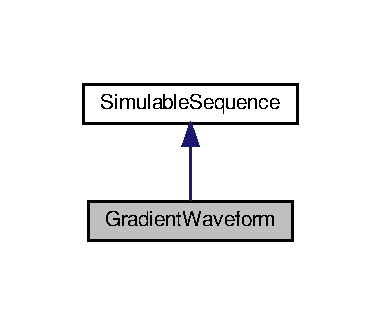
\includegraphics[width=183pt]{class_gradient_waveform__inherit__graph}
\end{center}
\end{figure}


Collaboration diagram for Gradient\+Waveform\+:\nopagebreak
\begin{figure}[H]
\begin{center}
\leavevmode
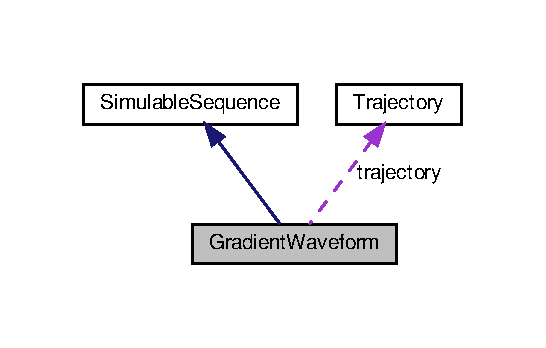
\includegraphics[width=262pt]{class_gradient_waveform__coll__graph}
\end{center}
\end{figure}
\subsection*{Public Member Functions}
\begin{DoxyCompactItemize}
\item 
\mbox{\Hypertarget{class_gradient_waveform_acf951c9a86f95d002db4858ee4c78582}\label{class_gradient_waveform_acf951c9a86f95d002db4858ee4c78582}} 
\hyperlink{class_gradient_waveform_acf951c9a86f95d002db4858ee4c78582}{Gradient\+Waveform} ()
\begin{DoxyCompactList}\small\item\em Default constructor, set default N\+U\+LL values. Not to be used. \end{DoxyCompactList}\item 
\mbox{\Hypertarget{class_gradient_waveform_aad3922dbe19647ed0fcbba175fb9a5ff}\label{class_gradient_waveform_aad3922dbe19647ed0fcbba175fb9a5ff}} 
\hyperlink{class_gradient_waveform_aad3922dbe19647ed0fcbba175fb9a5ff}{Gradient\+Waveform} (\hyperlink{class_scheme}{Scheme} \&scheme)
\begin{DoxyCompactList}\small\item\em Main constructor. Takes a pre-\/loaded \hyperlink{class_scheme}{Scheme} file. \end{DoxyCompactList}\item 
\mbox{\Hypertarget{class_gradient_waveform_a4780653a03ac1f576aeb6102b910ccde}\label{class_gradient_waveform_a4780653a03ac1f576aeb6102b910ccde}} 
\hyperlink{class_gradient_waveform_a4780653a03ac1f576aeb6102b910ccde}{Gradient\+Waveform} (\hyperlink{class_scheme}{Scheme} \&scheme\+\_\+, const char $\ast$traj\+\_\+file\+\_\+name)
\begin{DoxyCompactList}\small\item\em Main constructor. Takes a pre-\/loaded \hyperlink{class_scheme}{Scheme} file and a traj file name. if this argument is passed a traj file is should be written. \end{DoxyCompactList}\item 
double \hyperlink{class_gradient_waveform_a5f55e43b3057509b0f98812d2a72db9a}{get\+Numericalb\+Value} (unsigned)
\item 
\mbox{\Hypertarget{class_gradient_waveform_a52971b5f773c8c0b7c43bcd5fc50197a}\label{class_gradient_waveform_a52971b5f773c8c0b7c43bcd5fc50197a}} 
void \hyperlink{class_gradient_waveform_a52971b5f773c8c0b7c43bcd5fc50197a}{get\+D\+W\+I\+Signal} ()
\begin{DoxyCompactList}\small\item\em Computes de DW signal from a trajfile. \end{DoxyCompactList}\item 
\mbox{\Hypertarget{class_gradient_waveform_a82da8e7b3bffe4557e6e38191b7f8d81}\label{class_gradient_waveform_a82da8e7b3bffe4557e6e38191b7f8d81}} 
void \hyperlink{class_gradient_waveform_a82da8e7b3bffe4557e6e38191b7f8d81}{read\+Scheme\+File} ()
\begin{DoxyCompactList}\small\item\em reads the waveform \end{DoxyCompactList}\item 
\mbox{\Hypertarget{class_gradient_waveform_a2f1449c026649e4601f773086d1346ce}\label{class_gradient_waveform_a2f1449c026649e4601f773086d1346ce}} 
void \hyperlink{class_gradient_waveform_a2f1449c026649e4601f773086d1346ce}{get\+Interpolated\+Grad\+Impulse} (uint rep\+\_\+index, double dt\+\_\+sim, double t\+\_\+sim\+\_\+last, Eigen\+::\+Vector3d \&Gdt)
\begin{DoxyCompactList}\small\item\em For using with the adt array. \end{DoxyCompactList}\item 
void \hyperlink{class_gradient_waveform_a2c606400c648cebd85827efa8d22b6bc}{update\+\_\+phase\+\_\+shift} (double time\+\_\+step, Eigen\+::\+Matrix3\+Xd \hyperlink{class_gradient_waveform_a83a7c844f86acee3b7ab12e7e70202af}{trajectory})
\item 
void \hyperlink{class_gradient_waveform_a7421301b24b6c98e28ef9430287cdf8e}{update\+\_\+phase\+\_\+shift} (double \hyperlink{class_gradient_waveform_a3eacca54a58dc574384f07899a9a6da3}{dt}, double dt\+\_\+last, \hyperlink{class_walker}{Walker} walker)
\item 
\mbox{\Hypertarget{class_gradient_waveform_af4291596da9c45247b0748d945bd9b54}\label{class_gradient_waveform_af4291596da9c45247b0748d945bd9b54}} 
void \hyperlink{class_gradient_waveform_af4291596da9c45247b0748d945bd9b54}{update\+\_\+\+D\+W\+I\+\_\+signal} (\hyperlink{class_walker}{Walker} \&walker)
\begin{DoxyCompactList}\small\item\em Updates the D\+WI signal using the cumulated phase shift. \end{DoxyCompactList}\item 
\mbox{\Hypertarget{class_gradient_waveform_a040d4a70dc7951c235010791e1c581d1}\label{class_gradient_waveform_a040d4a70dc7951c235010791e1c581d1}} 
void \hyperlink{class_gradient_waveform_a040d4a70dc7951c235010791e1c581d1}{set\+Number\+Of\+Steps} (unsigned \hyperlink{class_gradient_waveform_af2f45ff237ba41afe3ff5cedb7c1c966}{T})
\begin{DoxyCompactList}\small\item\em Set the number of time steps if they are known. \end{DoxyCompactList}\item 
void \hyperlink{class_gradient_waveform_a80dd810cb4e5a11dec311ac87e55ea18}{get\+Grad\+Impulse} (int i, double t, double t\+Last, Eigen\+::\+Vector3d \&Gdt)
\end{DoxyCompactItemize}
\subsection*{Public Attributes}
\begin{DoxyCompactItemize}
\item 
int \hyperlink{class_gradient_waveform_a25edbe4ee53950831074f2ca4bfca48f}{num\+\_\+rep}
\item 
double \hyperlink{class_gradient_waveform_a4e0c0163e36cc017f5b147e9ca3022e0}{TE}
\item 
uint \hyperlink{class_gradient_waveform_af2f45ff237ba41afe3ff5cedb7c1c966}{T}
\item 
double \hyperlink{class_gradient_waveform_a8608216ab7e5f002dcf6af4f869c5d27}{dyn\+\_\+duration}
\item 
int \hyperlink{class_gradient_waveform_ac2287a6ef99e35f0c1f97fc3ffb37d7b}{wave\+\_\+bins}
\item 
double \hyperlink{class_gradient_waveform_a02d695fa36713bd28d3c85d2bb7a877b}{wave\+\_\+duration}
\item 
double \hyperlink{class_gradient_waveform_a3eacca54a58dc574384f07899a9a6da3}{dt}
\item 
bool \hyperlink{class_gradient_waveform_a712eedb2165b3f889e27244fc9d91ebd}{scale\+\_\+from\+\_\+stu}
\item 
std\+::vector$<$ std\+::vector$<$ float $>$ $>$ \hyperlink{class_gradient_waveform_a565fce08abb28fe26664194c04faeaea}{waveform}
\item 
\hyperlink{class_trajectory}{Trajectory} \hyperlink{class_gradient_waveform_a83a7c844f86acee3b7ab12e7e70202af}{trajectory}
\end{DoxyCompactItemize}


\subsection{Detailed Description}
Gradient Wavefroms =============================================================/. 

Implementation of the the General Wavefroms.

Main implementation of the gradient waveforms protocol \begin{DoxyAuthor}{Author}
Jonathan Rafael 
\end{DoxyAuthor}
\begin{DoxyDate}{Date}
November 2017 \subsection*{1.\+42 }
\end{DoxyDate}


\subsection{Member Function Documentation}
\mbox{\Hypertarget{class_gradient_waveform_a80dd810cb4e5a11dec311ac87e55ea18}\label{class_gradient_waveform_a80dd810cb4e5a11dec311ac87e55ea18}} 
\index{Gradient\+Waveform@{Gradient\+Waveform}!get\+Grad\+Impulse@{get\+Grad\+Impulse}}
\index{get\+Grad\+Impulse@{get\+Grad\+Impulse}!Gradient\+Waveform@{Gradient\+Waveform}}
\subsubsection{\texorpdfstring{get\+Grad\+Impulse()}{getGradImpulse()}}
{\footnotesize\ttfamily void Gradient\+Waveform\+::get\+Grad\+Impulse (\begin{DoxyParamCaption}\item[{int}]{i,  }\item[{double}]{t,  }\item[{double}]{t\+Last,  }\item[{Eigen\+::\+Vector3d \&}]{Gdt }\end{DoxyParamCaption})\hspace{0.3cm}{\ttfamily [virtual]}}


\begin{DoxyParams}{Parameters}
{\em i} & \hyperlink{class_walker}{Walker} index \\
\hline
{\em t} & current time step (in milisenconds) \\
\hline
{\em t\+Last} & last time step (in milisenconds) \\
\hline
{\em Gdt} & vector to compute de G$\ast$dt impulse \\
\hline
\end{DoxyParams}


Implements \hyperlink{class_simulable_sequence_a03a417776f5404b06c761ab9109e3e1d}{Simulable\+Sequence}.

\mbox{\Hypertarget{class_gradient_waveform_a5f55e43b3057509b0f98812d2a72db9a}\label{class_gradient_waveform_a5f55e43b3057509b0f98812d2a72db9a}} 
\index{Gradient\+Waveform@{Gradient\+Waveform}!get\+Numericalb\+Value@{get\+Numericalb\+Value}}
\index{get\+Numericalb\+Value@{get\+Numericalb\+Value}!Gradient\+Waveform@{Gradient\+Waveform}}
\subsubsection{\texorpdfstring{get\+Numericalb\+Value()}{getNumericalbValue()}}
{\footnotesize\ttfamily double Gradient\+Waveform\+::get\+Numericalb\+Value (\begin{DoxyParamCaption}\item[{unsigned}]{ }\end{DoxyParamCaption})}

\begin{DoxyWarning}{Warning}
not implemented yet. 
\end{DoxyWarning}
\mbox{\Hypertarget{class_gradient_waveform_a2c606400c648cebd85827efa8d22b6bc}\label{class_gradient_waveform_a2c606400c648cebd85827efa8d22b6bc}} 
\index{Gradient\+Waveform@{Gradient\+Waveform}!update\+\_\+phase\+\_\+shift@{update\+\_\+phase\+\_\+shift}}
\index{update\+\_\+phase\+\_\+shift@{update\+\_\+phase\+\_\+shift}!Gradient\+Waveform@{Gradient\+Waveform}}
\subsubsection{\texorpdfstring{update\+\_\+phase\+\_\+shift()}{update\_phase\_shift()}\hspace{0.1cm}{\footnotesize\ttfamily [1/2]}}
{\footnotesize\ttfamily void Gradient\+Waveform\+::update\+\_\+phase\+\_\+shift (\begin{DoxyParamCaption}\item[{double}]{time\+\_\+step,  }\item[{Eigen\+::\+Matrix3\+Xd}]{trajectory }\end{DoxyParamCaption})\hspace{0.3cm}{\ttfamily [virtual]}}


\begin{DoxyParams}{Parameters}
{\em i} & updated the phase shift over a whole trajectory \\
\hline
\end{DoxyParams}


Implements \hyperlink{class_simulable_sequence_a175197d165ee7852094bc70cadc59589}{Simulable\+Sequence}.

\mbox{\Hypertarget{class_gradient_waveform_a7421301b24b6c98e28ef9430287cdf8e}\label{class_gradient_waveform_a7421301b24b6c98e28ef9430287cdf8e}} 
\index{Gradient\+Waveform@{Gradient\+Waveform}!update\+\_\+phase\+\_\+shift@{update\+\_\+phase\+\_\+shift}}
\index{update\+\_\+phase\+\_\+shift@{update\+\_\+phase\+\_\+shift}!Gradient\+Waveform@{Gradient\+Waveform}}
\subsubsection{\texorpdfstring{update\+\_\+phase\+\_\+shift()}{update\_phase\_shift()}\hspace{0.1cm}{\footnotesize\ttfamily [2/2]}}
{\footnotesize\ttfamily void Gradient\+Waveform\+::update\+\_\+phase\+\_\+shift (\begin{DoxyParamCaption}\item[{double}]{dt,  }\item[{double}]{dt\+\_\+last,  }\item[{\hyperlink{class_walker}{Walker}}]{walker }\end{DoxyParamCaption})\hspace{0.3cm}{\ttfamily [virtual]}}


\begin{DoxyParams}{Parameters}
{\em i} & updated walker \\
\hline
\end{DoxyParams}


Implements \hyperlink{class_simulable_sequence_ad7b2a30f563343aa65489aa553d4df63}{Simulable\+Sequence}.



\subsection{Member Data Documentation}
\mbox{\Hypertarget{class_gradient_waveform_a3eacca54a58dc574384f07899a9a6da3}\label{class_gradient_waveform_a3eacca54a58dc574384f07899a9a6da3}} 
\index{Gradient\+Waveform@{Gradient\+Waveform}!dt@{dt}}
\index{dt@{dt}!Gradient\+Waveform@{Gradient\+Waveform}}
\subsubsection{\texorpdfstring{dt}{dt}}
{\footnotesize\ttfamily double Gradient\+Waveform\+::dt}

individual time steps (miliseconds) of the wave \mbox{\Hypertarget{class_gradient_waveform_a8608216ab7e5f002dcf6af4f869c5d27}\label{class_gradient_waveform_a8608216ab7e5f002dcf6af4f869c5d27}} 
\index{Gradient\+Waveform@{Gradient\+Waveform}!dyn\+\_\+duration@{dyn\+\_\+duration}}
\index{dyn\+\_\+duration@{dyn\+\_\+duration}!Gradient\+Waveform@{Gradient\+Waveform}}
\subsubsection{\texorpdfstring{dyn\+\_\+duration}{dyn\_duration}}
{\footnotesize\ttfamily double Gradient\+Waveform\+::dyn\+\_\+duration}

simulation duration (miliseconds) \mbox{\Hypertarget{class_gradient_waveform_a25edbe4ee53950831074f2ca4bfca48f}\label{class_gradient_waveform_a25edbe4ee53950831074f2ca4bfca48f}} 
\index{Gradient\+Waveform@{Gradient\+Waveform}!num\+\_\+rep@{num\+\_\+rep}}
\index{num\+\_\+rep@{num\+\_\+rep}!Gradient\+Waveform@{Gradient\+Waveform}}
\subsubsection{\texorpdfstring{num\+\_\+rep}{num\_rep}}
{\footnotesize\ttfamily int Gradient\+Waveform\+::num\+\_\+rep}

number of repetitions . \mbox{\Hypertarget{class_gradient_waveform_a712eedb2165b3f889e27244fc9d91ebd}\label{class_gradient_waveform_a712eedb2165b3f889e27244fc9d91ebd}} 
\index{Gradient\+Waveform@{Gradient\+Waveform}!scale\+\_\+from\+\_\+stu@{scale\+\_\+from\+\_\+stu}}
\index{scale\+\_\+from\+\_\+stu@{scale\+\_\+from\+\_\+stu}!Gradient\+Waveform@{Gradient\+Waveform}}
\subsubsection{\texorpdfstring{scale\+\_\+from\+\_\+stu}{scale\_from\_stu}}
{\footnotesize\ttfamily bool Gradient\+Waveform\+::scale\+\_\+from\+\_\+stu}

True if the input is in standar units \mbox{\Hypertarget{class_gradient_waveform_af2f45ff237ba41afe3ff5cedb7c1c966}\label{class_gradient_waveform_af2f45ff237ba41afe3ff5cedb7c1c966}} 
\index{Gradient\+Waveform@{Gradient\+Waveform}!T@{T}}
\index{T@{T}!Gradient\+Waveform@{Gradient\+Waveform}}
\subsubsection{\texorpdfstring{T}{T}}
{\footnotesize\ttfamily uint Gradient\+Waveform\+::T}

num bins (time steps) \mbox{\Hypertarget{class_gradient_waveform_a4e0c0163e36cc017f5b147e9ca3022e0}\label{class_gradient_waveform_a4e0c0163e36cc017f5b147e9ca3022e0}} 
\index{Gradient\+Waveform@{Gradient\+Waveform}!TE@{TE}}
\index{TE@{TE}!Gradient\+Waveform@{Gradient\+Waveform}}
\subsubsection{\texorpdfstring{TE}{TE}}
{\footnotesize\ttfamily double Gradient\+Waveform\+::\+TE}

Time Echo. \mbox{\Hypertarget{class_gradient_waveform_a83a7c844f86acee3b7ab12e7e70202af}\label{class_gradient_waveform_a83a7c844f86acee3b7ab12e7e70202af}} 
\index{Gradient\+Waveform@{Gradient\+Waveform}!trajectory@{trajectory}}
\index{trajectory@{trajectory}!Gradient\+Waveform@{Gradient\+Waveform}}
\subsubsection{\texorpdfstring{trajectory}{trajectory}}
{\footnotesize\ttfamily \hyperlink{class_trajectory}{Trajectory} Gradient\+Waveform\+::trajectory}

If the signal is computed from a .trajfile \mbox{\Hypertarget{class_gradient_waveform_ac2287a6ef99e35f0c1f97fc3ffb37d7b}\label{class_gradient_waveform_ac2287a6ef99e35f0c1f97fc3ffb37d7b}} 
\index{Gradient\+Waveform@{Gradient\+Waveform}!wave\+\_\+bins@{wave\+\_\+bins}}
\index{wave\+\_\+bins@{wave\+\_\+bins}!Gradient\+Waveform@{Gradient\+Waveform}}
\subsubsection{\texorpdfstring{wave\+\_\+bins}{wave\_bins}}
{\footnotesize\ttfamily int Gradient\+Waveform\+::wave\+\_\+bins}

Wave discretization \mbox{\Hypertarget{class_gradient_waveform_a02d695fa36713bd28d3c85d2bb7a877b}\label{class_gradient_waveform_a02d695fa36713bd28d3c85d2bb7a877b}} 
\index{Gradient\+Waveform@{Gradient\+Waveform}!wave\+\_\+duration@{wave\+\_\+duration}}
\index{wave\+\_\+duration@{wave\+\_\+duration}!Gradient\+Waveform@{Gradient\+Waveform}}
\subsubsection{\texorpdfstring{wave\+\_\+duration}{wave\_duration}}
{\footnotesize\ttfamily double Gradient\+Waveform\+::wave\+\_\+duration}

Wave duration (should be less qeual than dyn\+\_\+dur.) \mbox{\Hypertarget{class_gradient_waveform_a565fce08abb28fe26664194c04faeaea}\label{class_gradient_waveform_a565fce08abb28fe26664194c04faeaea}} 
\index{Gradient\+Waveform@{Gradient\+Waveform}!waveform@{waveform}}
\index{waveform@{waveform}!Gradient\+Waveform@{Gradient\+Waveform}}
\subsubsection{\texorpdfstring{waveform}{waveform}}
{\footnotesize\ttfamily std\+::vector$<$ std\+::vector$<$float$>$ $>$ Gradient\+Waveform\+::waveform}

Defined waveforms 

The documentation for this class was generated from the following files\+:\begin{DoxyCompactItemize}
\item 
src/gradientwaveform.\+h\item 
src/gradientwaveform.\+cpp\end{DoxyCompactItemize}

\hypertarget{class_m_c_simulation}{}\section{M\+C\+Simulation Class Reference}
\label{class_m_c_simulation}\index{M\+C\+Simulation@{M\+C\+Simulation}}


Aplication Main Class ======================================================================================/.  




{\ttfamily \#include $<$mcsimulation.\+h$>$}



Collaboration diagram for M\+C\+Simulation\+:
\nopagebreak
\begin{figure}[H]
\begin{center}
\leavevmode
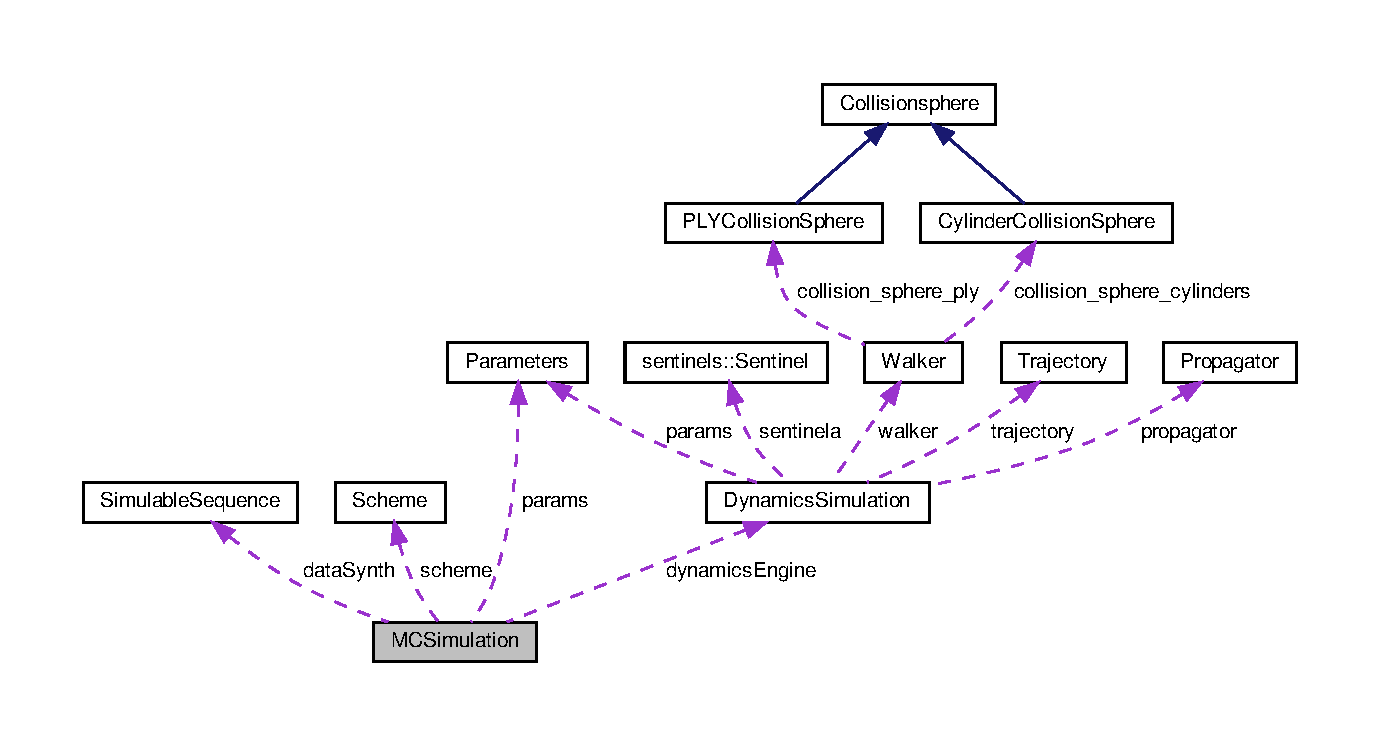
\includegraphics[width=350pt]{class_m_c_simulation__coll__graph}
\end{center}
\end{figure}
\subsection*{Public Member Functions}
\begin{DoxyCompactItemize}
\item 
\hyperlink{class_m_c_simulation_a89f56682a13f0bcb2c53d191ca336e35}{M\+C\+Simulation} ()
\begin{DoxyCompactList}\small\item\em Default constructor. Intialize everything with 0\textquotesingle{}s and N\+U\+LL states, object indexes are set to -\/1. \end{DoxyCompactList}\item 
\mbox{\Hypertarget{class_m_c_simulation_a5b2bdb95de31810a0d2ee54174e83f98}\label{class_m_c_simulation_a5b2bdb95de31810a0d2ee54174e83f98}} 
{\bfseries M\+C\+Simulation} (std\+::string config\+\_\+file)
\item 
\mbox{\Hypertarget{class_m_c_simulation_a76ac3d50d345d249cacc913273b2bd34}\label{class_m_c_simulation_a76ac3d50d345d249cacc913273b2bd34}} 
{\bfseries M\+C\+Simulation} (\hyperlink{class_parameters}{Parameters} \&params\+\_\+)
\item 
\mbox{\Hypertarget{class_m_c_simulation_a859c6ddce0e3c07db0159b2e4906b7ca}\label{class_m_c_simulation_a859c6ddce0e3c07db0159b2e4906b7ca}} 
\hyperlink{class_m_c_simulation_a859c6ddce0e3c07db0159b2e4906b7ca}{$\sim$\+M\+C\+Simulation} ()
\begin{DoxyCompactList}\small\item\em Main destructor. Frees dynamicly allocated memory instances. \end{DoxyCompactList}\item 
void \hyperlink{class_m_c_simulation_aa305f18bd48dd26f916cc9c006a8dec8}{start\+Simulation} ()
\begin{DoxyCompactList}\small\item\em Warp function. Calls the dynamic\+Engine\textquotesingle{}s native \hyperlink{class_dynamics_simulation_a00cf4a6cbde1ef708fdbd58e8d8a7727}{Dynamics\+Simulation\+::start\+Simulation} function. \end{DoxyCompactList}\item 
\mbox{\Hypertarget{class_m_c_simulation_aff302334b2743a583b5d6f642d841f2f}\label{class_m_c_simulation_aff302334b2743a583b5d6f642d841f2f}} 
double {\bfseries get\+Expected\+Freee\+Decay} (unsigned i)
\item 
void \hyperlink{class_m_c_simulation_aa60234e3f6d2a100c8b03e4f304b07f4}{ini\+Obstacles} ()
\end{DoxyCompactItemize}
\subsection*{Public Attributes}
\begin{DoxyCompactItemize}
\item 
int \hyperlink{class_m_c_simulation_aff828a83a905ae188146d3ffaa12a1bc}{id}
\item 
\hyperlink{class_dynamics_simulation}{Dynamics\+Simulation} $\ast$ \hyperlink{class_m_c_simulation_ac453455b2dfb994b7b1a4b7823bd3dc9}{dynamics\+Engine}
\item 
\hyperlink{class_scheme}{Scheme} \hyperlink{class_m_c_simulation_a87ba6332f1f49024a442981b477360c4}{scheme}
\item 
\hyperlink{class_parameters}{Parameters} \hyperlink{class_m_c_simulation_aecb8470cb31fa67e38c5d5acd5a80bef}{params}
\item 
\hyperlink{class_simulable_sequence}{Simulable\+Sequence} $\ast$ \hyperlink{class_m_c_simulation_a7e2496127af6436d64bca7f52bc40c82}{data\+Synth}
\item 
std\+::vector$<$ std\+::vector$<$ float $>$ $>$ \hyperlink{class_m_c_simulation_af53387a4edc7627a77ff03a562f8befa}{ini\+\_\+walker\+\_\+positions}
\item 
std\+::vector$<$ \hyperlink{class_p_l_y_obstacle}{P\+L\+Y\+Obstacle} $>$ $\ast$ \hyperlink{class_m_c_simulation_a8c21d28d54c9c947f6c5465657019ed4}{ply\+Obstacles\+\_\+list}
\item 
std\+::vector$<$ \hyperlink{class_cylinder}{Cylinder} $>$ $\ast$ \hyperlink{class_m_c_simulation_a36909899f67439feed1a980037ea8c03}{cylinders\+\_\+list}
\end{DoxyCompactItemize}
\subsection*{Static Public Attributes}
\begin{DoxyCompactItemize}
\item 
static int \hyperlink{class_m_c_simulation_aa3853b6cec83b055593cbf58def0c164}{count} =0
\end{DoxyCompactItemize}


\subsection{Detailed Description}
Aplication Main Class ======================================================================================/. 

Main implementation class. Incorporates the particle\textquotesingle{}s dynamics and the data synthesis. \begin{DoxyAuthor}{Author}
Jonathan Rafael 
\end{DoxyAuthor}
\begin{DoxyDate}{Date}
November 2016 \subsection*{1.\+44.\+00 }
\end{DoxyDate}


Main implementation class. Incorporates the particle\textquotesingle{}s dynamics and the data synthesis. 

\subsection{Constructor \& Destructor Documentation}
\mbox{\Hypertarget{class_m_c_simulation_a89f56682a13f0bcb2c53d191ca336e35}\label{class_m_c_simulation_a89f56682a13f0bcb2c53d191ca336e35}} 
\index{M\+C\+Simulation@{M\+C\+Simulation}!M\+C\+Simulation@{M\+C\+Simulation}}
\index{M\+C\+Simulation@{M\+C\+Simulation}!M\+C\+Simulation@{M\+C\+Simulation}}
\subsubsection{\texorpdfstring{M\+C\+Simulation()}{MCSimulation()}}
{\footnotesize\ttfamily M\+C\+Simulation\+::\+M\+C\+Simulation (\begin{DoxyParamCaption}{ }\end{DoxyParamCaption})}



Default constructor. Intialize everything with 0\textquotesingle{}s and N\+U\+LL states, object indexes are set to -\/1. 

Secondary constructor.

Main constructor.


\begin{DoxyParams}{Parameters}
{\em config\+\_\+file} & .conf file name with the full set of experiments parameters.\\
\hline
{\em params\+\_\+} & preloaded simulation parameters. \\
\hline
\end{DoxyParams}


\subsection{Member Function Documentation}
\mbox{\Hypertarget{class_m_c_simulation_aa60234e3f6d2a100c8b03e4f304b07f4}\label{class_m_c_simulation_aa60234e3f6d2a100c8b03e4f304b07f4}} 
\index{M\+C\+Simulation@{M\+C\+Simulation}!ini\+Obstacles@{ini\+Obstacles}}
\index{ini\+Obstacles@{ini\+Obstacles}!M\+C\+Simulation@{M\+C\+Simulation}}
\subsubsection{\texorpdfstring{ini\+Obstacles()}{iniObstacles()}}
{\footnotesize\ttfamily void M\+C\+Simulation\+::ini\+Obstacles (\begin{DoxyParamCaption}{ }\end{DoxyParamCaption})}

Adds all the obstacles defined in the confiuration files. \mbox{\Hypertarget{class_m_c_simulation_aa305f18bd48dd26f916cc9c006a8dec8}\label{class_m_c_simulation_aa305f18bd48dd26f916cc9c006a8dec8}} 
\index{M\+C\+Simulation@{M\+C\+Simulation}!start\+Simulation@{start\+Simulation}}
\index{start\+Simulation@{start\+Simulation}!M\+C\+Simulation@{M\+C\+Simulation}}
\subsubsection{\texorpdfstring{start\+Simulation()}{startSimulation()}}
{\footnotesize\ttfamily M\+C\+Simulation\+::start\+Simulation (\begin{DoxyParamCaption}{ }\end{DoxyParamCaption})}



Warp function. Calls the dynamic\+Engine\textquotesingle{}s native \hyperlink{class_dynamics_simulation_a00cf4a6cbde1ef708fdbd58e8d8a7727}{Dynamics\+Simulation\+::start\+Simulation} function. 

\begin{DoxySeeAlso}{See also}
\+:\hyperlink{class_dynamics_simulation}{Dynamics\+Simulation}\+:. 
\end{DoxySeeAlso}


\subsection{Member Data Documentation}
\mbox{\Hypertarget{class_m_c_simulation_aa3853b6cec83b055593cbf58def0c164}\label{class_m_c_simulation_aa3853b6cec83b055593cbf58def0c164}} 
\index{M\+C\+Simulation@{M\+C\+Simulation}!count@{count}}
\index{count@{count}!M\+C\+Simulation@{M\+C\+Simulation}}
\subsubsection{\texorpdfstring{count}{count}}
{\footnotesize\ttfamily int M\+C\+Simulation\+::count =0\hspace{0.3cm}{\ttfamily [static]}}

count of \mbox{\Hypertarget{class_m_c_simulation_a36909899f67439feed1a980037ea8c03}\label{class_m_c_simulation_a36909899f67439feed1a980037ea8c03}} 
\index{M\+C\+Simulation@{M\+C\+Simulation}!cylinders\+\_\+list@{cylinders\+\_\+list}}
\index{cylinders\+\_\+list@{cylinders\+\_\+list}!M\+C\+Simulation@{M\+C\+Simulation}}
\subsubsection{\texorpdfstring{cylinders\+\_\+list}{cylinders\_list}}
{\footnotesize\ttfamily std\+::vector$<$\hyperlink{class_cylinder}{Cylinder}$>$$\ast$ M\+C\+Simulation\+::cylinders\+\_\+list}

pointer to a vector with all the instances of Cylinders \mbox{\Hypertarget{class_m_c_simulation_a7e2496127af6436d64bca7f52bc40c82}\label{class_m_c_simulation_a7e2496127af6436d64bca7f52bc40c82}} 
\index{M\+C\+Simulation@{M\+C\+Simulation}!data\+Synth@{data\+Synth}}
\index{data\+Synth@{data\+Synth}!M\+C\+Simulation@{M\+C\+Simulation}}
\subsubsection{\texorpdfstring{data\+Synth}{dataSynth}}
{\footnotesize\ttfamily \hyperlink{class_simulable_sequence}{Simulable\+Sequence}$\ast$ M\+C\+Simulation\+::data\+Synth}

Simuleable sequence instance, P\+G\+SE and General Wavefroms only \mbox{\Hypertarget{class_m_c_simulation_ac453455b2dfb994b7b1a4b7823bd3dc9}\label{class_m_c_simulation_ac453455b2dfb994b7b1a4b7823bd3dc9}} 
\index{M\+C\+Simulation@{M\+C\+Simulation}!dynamics\+Engine@{dynamics\+Engine}}
\index{dynamics\+Engine@{dynamics\+Engine}!M\+C\+Simulation@{M\+C\+Simulation}}
\subsubsection{\texorpdfstring{dynamics\+Engine}{dynamicsEngine}}
{\footnotesize\ttfamily \hyperlink{class_dynamics_simulation}{Dynamics\+Simulation}$\ast$ M\+C\+Simulation\+::dynamics\+Engine}

Instance for the particle dynamics \mbox{\Hypertarget{class_m_c_simulation_aff828a83a905ae188146d3ffaa12a1bc}\label{class_m_c_simulation_aff828a83a905ae188146d3ffaa12a1bc}} 
\index{M\+C\+Simulation@{M\+C\+Simulation}!id@{id}}
\index{id@{id}!M\+C\+Simulation@{M\+C\+Simulation}}
\subsubsection{\texorpdfstring{id}{id}}
{\footnotesize\ttfamily int M\+C\+Simulation\+::id}

Unique id of the simulation \mbox{\Hypertarget{class_m_c_simulation_af53387a4edc7627a77ff03a562f8befa}\label{class_m_c_simulation_af53387a4edc7627a77ff03a562f8befa}} 
\index{M\+C\+Simulation@{M\+C\+Simulation}!ini\+\_\+walker\+\_\+positions@{ini\+\_\+walker\+\_\+positions}}
\index{ini\+\_\+walker\+\_\+positions@{ini\+\_\+walker\+\_\+positions}!M\+C\+Simulation@{M\+C\+Simulation}}
\subsubsection{\texorpdfstring{ini\+\_\+walker\+\_\+positions}{ini\_walker\_positions}}
{\footnotesize\ttfamily std\+::vector$<$std\+::vector$<$float$>$ $>$ M\+C\+Simulation\+::ini\+\_\+walker\+\_\+positions}

patch for regular sampling in a subdivision \mbox{\Hypertarget{class_m_c_simulation_aecb8470cb31fa67e38c5d5acd5a80bef}\label{class_m_c_simulation_aecb8470cb31fa67e38c5d5acd5a80bef}} 
\index{M\+C\+Simulation@{M\+C\+Simulation}!params@{params}}
\index{params@{params}!M\+C\+Simulation@{M\+C\+Simulation}}
\subsubsection{\texorpdfstring{params}{params}}
{\footnotesize\ttfamily \hyperlink{class_parameters}{Parameters} M\+C\+Simulation\+::params}

\hyperlink{class_parameters}{Parameters} instance1 \begin{DoxySeeAlso}{See also}
\+:\hyperlink{class_parameters}{Parameters}\+: 
\end{DoxySeeAlso}
\mbox{\Hypertarget{class_m_c_simulation_a8c21d28d54c9c947f6c5465657019ed4}\label{class_m_c_simulation_a8c21d28d54c9c947f6c5465657019ed4}} 
\index{M\+C\+Simulation@{M\+C\+Simulation}!ply\+Obstacles\+\_\+list@{ply\+Obstacles\+\_\+list}}
\index{ply\+Obstacles\+\_\+list@{ply\+Obstacles\+\_\+list}!M\+C\+Simulation@{M\+C\+Simulation}}
\subsubsection{\texorpdfstring{ply\+Obstacles\+\_\+list}{plyObstacles\_list}}
{\footnotesize\ttfamily std\+::vector$<$\hyperlink{class_p_l_y_obstacle}{P\+L\+Y\+Obstacle}$>$$\ast$ M\+C\+Simulation\+::ply\+Obstacles\+\_\+list}

pointer to a vector with all the instances of P\+L\+Y\+Obstacles \mbox{\Hypertarget{class_m_c_simulation_a87ba6332f1f49024a442981b477360c4}\label{class_m_c_simulation_a87ba6332f1f49024a442981b477360c4}} 
\index{M\+C\+Simulation@{M\+C\+Simulation}!scheme@{scheme}}
\index{scheme@{scheme}!M\+C\+Simulation@{M\+C\+Simulation}}
\subsubsection{\texorpdfstring{scheme}{scheme}}
{\footnotesize\ttfamily \hyperlink{class_scheme}{Scheme} M\+C\+Simulation\+::scheme}

\hyperlink{class_scheme}{Scheme} file, only P\+G\+SE in camino format is supported in 0.\+2 

The documentation for this class was generated from the following files\+:\begin{DoxyCompactItemize}
\item 
src/mcsimulation.\+h\item 
src/mcsimulation.\+cpp\end{DoxyCompactItemize}

\hypertarget{class_obstacle}{}\section{Obstacle Class Reference}
\label{class_obstacle}\index{Obstacle@{Obstacle}}


\hyperlink{class_obstacle}{Obstacle} Base Class ==============================================================================/.  




{\ttfamily \#include $<$obstacle.\+h$>$}



Inheritance diagram for Obstacle\+:
\nopagebreak
\begin{figure}[H]
\begin{center}
\leavevmode
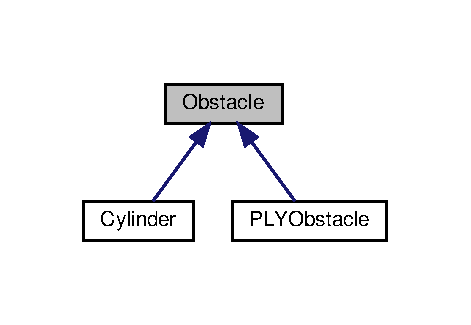
\includegraphics[width=226pt]{class_obstacle__inherit__graph}
\end{center}
\end{figure}
\subsection*{Public Member Functions}
\begin{DoxyCompactItemize}
\item 
\mbox{\Hypertarget{class_obstacle_a8f734072321fa06a7b7dae2d5f50f352}\label{class_obstacle_a8f734072321fa06a7b7dae2d5f50f352}} 
\hyperlink{class_obstacle_a8f734072321fa06a7b7dae2d5f50f352}{Obstacle} ()
\begin{DoxyCompactList}\small\item\em Default constructor. Does nothing. \end{DoxyCompactList}\item 
bool \hyperlink{class_obstacle_af11af63f11595304ff6d5c1785c03da5}{check\+Collision} (\hyperlink{class_walker}{Walker} \&walker, Eigen\+::\+Array3d \&step, const double \&step\+\_\+lenght, \hyperlink{class_collision}{Collision} \&colision)
\begin{DoxyCompactList}\small\item\em Basic collision function. Returns the if there was any collision on against the obstacle. \end{DoxyCompactList}\item 
\mbox{\Hypertarget{class_obstacle_a5316aabce6765c943d131aa3d5018f8d}\label{class_obstacle_a5316aabce6765c943d131aa3d5018f8d}} 
void {\bfseries elastic\+Bounce\+Agains\+Plane} (Eigen\+::\+Vector3d \&ray\+\_\+origin, Eigen\+::\+Vector3d \&normal, double \&t, Eigen\+::\+Vector3d \&step)
\item 
double \hyperlink{class_obstacle_a742e9d6ea940b33545cef4f1f2d58566}{min\+Distance} (\hyperlink{class_walker}{Walker} \&w)
\begin{DoxyCompactList}\small\item\em Returns the minimum distance of collision. \end{DoxyCompactList}\end{DoxyCompactItemize}
\subsection*{Public Attributes}
\begin{DoxyCompactItemize}
\item 
int \hyperlink{class_obstacle_a02e049a3395138a0dc6194af0112e2b0}{id}
\item 
int \hyperlink{class_obstacle_aaa096d441fd095c7bbe924d1a78a8e23}{count\+\_\+perc\+\_\+crossings}
\item 
double \hyperlink{class_obstacle_a7afe63ee05b482c526591c981b22cf54}{percolation}
\item 
double \hyperlink{class_obstacle_a374f9b4486f63abce9696f5fe3a13e8e}{T2}
\end{DoxyCompactItemize}


\subsection{Detailed Description}
\hyperlink{class_obstacle}{Obstacle} Base Class ==============================================================================/. 

Father class to define the base of any other obstacle (wall or substrate) \begin{DoxyAuthor}{Author}
Jonathan Rafael 
\end{DoxyAuthor}
\begin{DoxyDate}{Date}
November 2016 \subsection*{1.\+42 }
\end{DoxyDate}


\subsection{Member Function Documentation}
\mbox{\Hypertarget{class_obstacle_af11af63f11595304ff6d5c1785c03da5}\label{class_obstacle_af11af63f11595304ff6d5c1785c03da5}} 
\index{Obstacle@{Obstacle}!check\+Collision@{check\+Collision}}
\index{check\+Collision@{check\+Collision}!Obstacle@{Obstacle}}
\subsubsection{\texorpdfstring{check\+Collision()}{checkCollision()}}
{\footnotesize\ttfamily Obstacle\+::check\+Collision (\begin{DoxyParamCaption}\item[{\hyperlink{class_walker}{Walker} \&}]{walker,  }\item[{Eigen\+::\+Array3d \&}]{step,  }\item[{const double \&}]{step\+\_\+lenght,  }\item[{\hyperlink{class_collision}{Collision} \&}]{colision }\end{DoxyParamCaption})}



Basic collision function. Returns the if there was any collision on against the obstacle. 


\begin{DoxyParams}{Parameters}
{\em walker,\hyperlink{class_walker}{Walker}} & instance in the simulation. \\
\hline
{\em 3d} & step. Is assumed to be normalized. \\
\hline
{\em step\+\_\+lenght,length} & used as the maximum step collision distance. \\
\hline
{\em colilsion,\hyperlink{class_collision}{Collision}} & instance to save the collision (if any) details. \\
\hline
\end{DoxyParams}
\begin{DoxyReturn}{Returns}
true only if there was a Collision\+::hit status. 
\end{DoxyReturn}
\begin{DoxySeeAlso}{See also}
\hyperlink{class_collision}{Collision}. 
\end{DoxySeeAlso}
\mbox{\Hypertarget{class_obstacle_a742e9d6ea940b33545cef4f1f2d58566}\label{class_obstacle_a742e9d6ea940b33545cef4f1f2d58566}} 
\index{Obstacle@{Obstacle}!min\+Distance@{min\+Distance}}
\index{min\+Distance@{min\+Distance}!Obstacle@{Obstacle}}
\subsubsection{\texorpdfstring{min\+Distance()}{minDistance()}}
{\footnotesize\ttfamily double Obstacle\+::min\+Distance (\begin{DoxyParamCaption}\item[{\hyperlink{class_walker}{Walker} \&}]{w }\end{DoxyParamCaption})}



Returns the minimum distance of collision. 


\begin{DoxyParams}{Parameters}
{\em walker} & to find the (closest) distance. \\
\hline
\end{DoxyParams}


\subsection{Member Data Documentation}
\mbox{\Hypertarget{class_obstacle_aaa096d441fd095c7bbe924d1a78a8e23}\label{class_obstacle_aaa096d441fd095c7bbe924d1a78a8e23}} 
\index{Obstacle@{Obstacle}!count\+\_\+perc\+\_\+crossings@{count\+\_\+perc\+\_\+crossings}}
\index{count\+\_\+perc\+\_\+crossings@{count\+\_\+perc\+\_\+crossings}!Obstacle@{Obstacle}}
\subsubsection{\texorpdfstring{count\+\_\+perc\+\_\+crossings}{count\_perc\_crossings}}
{\footnotesize\ttfamily int Obstacle\+::count\+\_\+perc\+\_\+crossings}

Auxiliar value to count the number of percolatin crossings in a simulation \mbox{\Hypertarget{class_obstacle_a02e049a3395138a0dc6194af0112e2b0}\label{class_obstacle_a02e049a3395138a0dc6194af0112e2b0}} 
\index{Obstacle@{Obstacle}!id@{id}}
\index{id@{id}!Obstacle@{Obstacle}}
\subsubsection{\texorpdfstring{id}{id}}
{\footnotesize\ttfamily int Obstacle\+::id}

Unique id of the simulation \mbox{\Hypertarget{class_obstacle_a7afe63ee05b482c526591c981b22cf54}\label{class_obstacle_a7afe63ee05b482c526591c981b22cf54}} 
\index{Obstacle@{Obstacle}!percolation@{percolation}}
\index{percolation@{percolation}!Obstacle@{Obstacle}}
\subsubsection{\texorpdfstring{percolation}{percolation}}
{\footnotesize\ttfamily double Obstacle\+::percolation}

Percolation value between 0 and 1. \mbox{\Hypertarget{class_obstacle_a374f9b4486f63abce9696f5fe3a13e8e}\label{class_obstacle_a374f9b4486f63abce9696f5fe3a13e8e}} 
\index{Obstacle@{Obstacle}!T2@{T2}}
\index{T2@{T2}!Obstacle@{Obstacle}}
\subsubsection{\texorpdfstring{T2}{T2}}
{\footnotesize\ttfamily double Obstacle\+::\+T2}

T2 decay, not used by default 

The documentation for this class was generated from the following files\+:\begin{DoxyCompactItemize}
\item 
src/obstacle.\+h\item 
src/obstacle.\+cpp\end{DoxyCompactItemize}

\hypertarget{class_parallel_m_c_simulation}{}\section{Parallel\+M\+C\+Simulation Class Reference}
\label{class_parallel_m_c_simulation}\index{Parallel\+M\+C\+Simulation@{Parallel\+M\+C\+Simulation}}


Class to handle multiprocessor paralellisation. This class basicly controls and syncronize several initializations of Monte\+Carlo simulations and add up the results. It\textquotesingle{}s a way of soft paralelization.  




{\ttfamily \#include $<$parallelmcsimulation.\+h$>$}



Collaboration diagram for Parallel\+M\+C\+Simulation\+:
\nopagebreak
\begin{figure}[H]
\begin{center}
\leavevmode
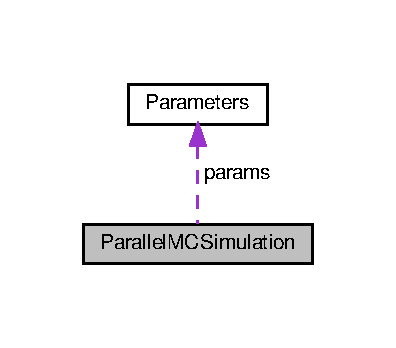
\includegraphics[width=190pt]{class_parallel_m_c_simulation__coll__graph}
\end{center}
\end{figure}
\subsection*{Public Member Functions}
\begin{DoxyCompactItemize}
\item 
\hyperlink{class_parallel_m_c_simulation_ac85dc215688a1462b770d20c2ff10b3f}{Parallel\+M\+C\+Simulation} (std\+::string config\+\_\+file)
\begin{DoxyCompactList}\small\item\em Main constructor. \end{DoxyCompactList}\item 
\hyperlink{class_parallel_m_c_simulation_a32ee405791787a1ea9d03895fdd810f4}{Parallel\+M\+C\+Simulation} (\hyperlink{class_parameters}{Parameters} \&\hyperlink{class_parallel_m_c_simulation_a83f856aaa88a403c657c7b8234deee7a}{params})
\begin{DoxyCompactList}\small\item\em Constructor. \end{DoxyCompactList}\item 
void \hyperlink{class_parallel_m_c_simulation_a7d9420ac20b19cb1c74f81bdbad94196}{start\+Simulation} ()
\begin{DoxyCompactList}\small\item\em Warp function. Calls the \hyperlink{class_m_c_simulation}{M\+C\+Simulation}\textquotesingle{}s native function for all the instances. \end{DoxyCompactList}\end{DoxyCompactItemize}
\subsection*{Public Attributes}
\begin{DoxyCompactItemize}
\item 
\hyperlink{class_parameters}{Parameters} \hyperlink{class_parallel_m_c_simulation_a83f856aaa88a403c657c7b8234deee7a}{params}
\item 
double \hyperlink{class_parallel_m_c_simulation_ad122df5454bb26a56e89c9077560a33d}{mean\+\_\+second\+\_\+passed}
\item 
unsigned \hyperlink{class_parallel_m_c_simulation_a18326e05c32fac82264d7351d78a7433}{total\+\_\+sim\+\_\+particles}
\item 
unsigned \hyperlink{class_parallel_m_c_simulation_a6ee1dfd6e695ec5ec7d4c2ed94f233cf}{stuck\+\_\+count}
\item 
unsigned \hyperlink{class_parallel_m_c_simulation_ae667ec358689a3a7b42876b401a5fce5}{illegal\+\_\+count}
\item 
double \hyperlink{class_parallel_m_c_simulation_a871e3fdace01984a533792dd49bebd1b}{icvf}
\item 
double \hyperlink{class_parallel_m_c_simulation_aa51edc0c79c6ae66ddd0046d21b871d4}{aprox\+\_\+volumen}
\item 
std\+::vector$<$ \hyperlink{class_m_c_simulation}{M\+C\+Simulation} $\ast$ $>$ \hyperlink{class_parallel_m_c_simulation_af16d292f007b8391122a035022422ed5}{simulations}
\item 
std\+::vector$<$ std\+::thread $>$ \hyperlink{class_parallel_m_c_simulation_a2a0f1cc2812c1a35e5e38d9d9ddde78b}{sim\+\_\+threads}
\item 
std\+::vector$<$ \hyperlink{class_p_l_y_obstacle}{P\+L\+Y\+Obstacle} $>$ \hyperlink{class_parallel_m_c_simulation_aa90f4d989bc868b6d225c0c5b9fe832a}{ply\+Obstacles\+\_\+list}
\item 
std\+::vector$<$ \hyperlink{class_cylinder}{Cylinder} $>$ \hyperlink{class_parallel_m_c_simulation_a4c36ff5327e9f19258fed5d64d48fdb8}{cylinders\+\_\+list}
\item 
std\+::vector$<$ Eigen\+::\+Vector3f $>$ \hyperlink{class_parallel_m_c_simulation_a5efe5faa45e57e6ff3827e9ec9e52a64}{total\+\_\+ini\+\_\+walker\+\_\+pos}
\end{DoxyCompactItemize}


\subsection{Detailed Description}
Class to handle multiprocessor paralellisation. This class basicly controls and syncronize several initializations of Monte\+Carlo simulations and add up the results. It\textquotesingle{}s a way of soft paralelization. 

Implementation of the P\+G\+SE protocol.

==============================================================================/

Class to handle multiprocessor paralellisation \begin{DoxyAuthor}{Author}
Jonathan Rafael 
\end{DoxyAuthor}
\begin{DoxyDate}{Date}
November 2016 

 
\end{DoxyDate}


\subsection{Constructor \& Destructor Documentation}
\mbox{\Hypertarget{class_parallel_m_c_simulation_ac85dc215688a1462b770d20c2ff10b3f}\label{class_parallel_m_c_simulation_ac85dc215688a1462b770d20c2ff10b3f}} 
\index{Parallel\+M\+C\+Simulation@{Parallel\+M\+C\+Simulation}!Parallel\+M\+C\+Simulation@{Parallel\+M\+C\+Simulation}}
\index{Parallel\+M\+C\+Simulation@{Parallel\+M\+C\+Simulation}!Parallel\+M\+C\+Simulation@{Parallel\+M\+C\+Simulation}}
\subsubsection{\texorpdfstring{Parallel\+M\+C\+Simulation()}{ParallelMCSimulation()}\hspace{0.1cm}{\footnotesize\ttfamily [1/2]}}
{\footnotesize\ttfamily Parallel\+M\+C\+Simulation\+::\+Parallel\+M\+C\+Simulation (\begin{DoxyParamCaption}\item[{std\+::string}]{config\+\_\+file }\end{DoxyParamCaption})}



Main constructor. 


\begin{DoxyParams}{Parameters}
{\em config\+\_\+file} & .conf file name with the full set of experiments parameters. \\
\hline
\end{DoxyParams}
\mbox{\Hypertarget{class_parallel_m_c_simulation_a32ee405791787a1ea9d03895fdd810f4}\label{class_parallel_m_c_simulation_a32ee405791787a1ea9d03895fdd810f4}} 
\index{Parallel\+M\+C\+Simulation@{Parallel\+M\+C\+Simulation}!Parallel\+M\+C\+Simulation@{Parallel\+M\+C\+Simulation}}
\index{Parallel\+M\+C\+Simulation@{Parallel\+M\+C\+Simulation}!Parallel\+M\+C\+Simulation@{Parallel\+M\+C\+Simulation}}
\subsubsection{\texorpdfstring{Parallel\+M\+C\+Simulation()}{ParallelMCSimulation()}\hspace{0.1cm}{\footnotesize\ttfamily [2/2]}}
{\footnotesize\ttfamily Parallel\+M\+C\+Simulation\+::\+Parallel\+M\+C\+Simulation (\begin{DoxyParamCaption}\item[{\hyperlink{class_parameters}{Parameters} \&}]{params }\end{DoxyParamCaption})}



Constructor. 


\begin{DoxyParams}{Parameters}
{\em parameters} & of the simulation. Read form a conf file or given by the user. \\
\hline
\end{DoxyParams}


\subsection{Member Function Documentation}
\mbox{\Hypertarget{class_parallel_m_c_simulation_a7d9420ac20b19cb1c74f81bdbad94196}\label{class_parallel_m_c_simulation_a7d9420ac20b19cb1c74f81bdbad94196}} 
\index{Parallel\+M\+C\+Simulation@{Parallel\+M\+C\+Simulation}!start\+Simulation@{start\+Simulation}}
\index{start\+Simulation@{start\+Simulation}!Parallel\+M\+C\+Simulation@{Parallel\+M\+C\+Simulation}}
\subsubsection{\texorpdfstring{start\+Simulation()}{startSimulation()}}
{\footnotesize\ttfamily Parallel\+M\+C\+Simulation\+::start\+Simulation (\begin{DoxyParamCaption}{ }\end{DoxyParamCaption})}



Warp function. Calls the \hyperlink{class_m_c_simulation}{M\+C\+Simulation}\textquotesingle{}s native function for all the instances. 

\begin{DoxySeeAlso}{See also}
\+:\hyperlink{class_m_c_simulation}{M\+C\+Simulation}\+:. 
\end{DoxySeeAlso}


\subsection{Member Data Documentation}
\mbox{\Hypertarget{class_parallel_m_c_simulation_aa51edc0c79c6ae66ddd0046d21b871d4}\label{class_parallel_m_c_simulation_aa51edc0c79c6ae66ddd0046d21b871d4}} 
\index{Parallel\+M\+C\+Simulation@{Parallel\+M\+C\+Simulation}!aprox\+\_\+volumen@{aprox\+\_\+volumen}}
\index{aprox\+\_\+volumen@{aprox\+\_\+volumen}!Parallel\+M\+C\+Simulation@{Parallel\+M\+C\+Simulation}}
\subsubsection{\texorpdfstring{aprox\+\_\+volumen}{aprox\_volumen}}
{\footnotesize\ttfamily double Parallel\+M\+C\+Simulation\+::aprox\+\_\+volumen}

Stores the volumen based on I\+C\+VF and the voxel size \mbox{\Hypertarget{class_parallel_m_c_simulation_a4c36ff5327e9f19258fed5d64d48fdb8}\label{class_parallel_m_c_simulation_a4c36ff5327e9f19258fed5d64d48fdb8}} 
\index{Parallel\+M\+C\+Simulation@{Parallel\+M\+C\+Simulation}!cylinders\+\_\+list@{cylinders\+\_\+list}}
\index{cylinders\+\_\+list@{cylinders\+\_\+list}!Parallel\+M\+C\+Simulation@{Parallel\+M\+C\+Simulation}}
\subsubsection{\texorpdfstring{cylinders\+\_\+list}{cylinders\_list}}
{\footnotesize\ttfamily std\+::vector$<$\hyperlink{class_cylinder}{Cylinder}$>$ Parallel\+M\+C\+Simulation\+::cylinders\+\_\+list}

vector with all the instances of cylinders \mbox{\Hypertarget{class_parallel_m_c_simulation_a871e3fdace01984a533792dd49bebd1b}\label{class_parallel_m_c_simulation_a871e3fdace01984a533792dd49bebd1b}} 
\index{Parallel\+M\+C\+Simulation@{Parallel\+M\+C\+Simulation}!icvf@{icvf}}
\index{icvf@{icvf}!Parallel\+M\+C\+Simulation@{Parallel\+M\+C\+Simulation}}
\subsubsection{\texorpdfstring{icvf}{icvf}}
{\footnotesize\ttfamily double Parallel\+M\+C\+Simulation\+::icvf}

Stores the I\+C\+VF based on the particles sampling \mbox{\Hypertarget{class_parallel_m_c_simulation_ae667ec358689a3a7b42876b401a5fce5}\label{class_parallel_m_c_simulation_ae667ec358689a3a7b42876b401a5fce5}} 
\index{Parallel\+M\+C\+Simulation@{Parallel\+M\+C\+Simulation}!illegal\+\_\+count@{illegal\+\_\+count}}
\index{illegal\+\_\+count@{illegal\+\_\+count}!Parallel\+M\+C\+Simulation@{Parallel\+M\+C\+Simulation}}
\subsubsection{\texorpdfstring{illegal\+\_\+count}{illegal\_count}}
{\footnotesize\ttfamily unsigned Parallel\+M\+C\+Simulation\+::illegal\+\_\+count}

Counts the number of particles that attempt to cross \mbox{\Hypertarget{class_parallel_m_c_simulation_ad122df5454bb26a56e89c9077560a33d}\label{class_parallel_m_c_simulation_ad122df5454bb26a56e89c9077560a33d}} 
\index{Parallel\+M\+C\+Simulation@{Parallel\+M\+C\+Simulation}!mean\+\_\+second\+\_\+passed@{mean\+\_\+second\+\_\+passed}}
\index{mean\+\_\+second\+\_\+passed@{mean\+\_\+second\+\_\+passed}!Parallel\+M\+C\+Simulation@{Parallel\+M\+C\+Simulation}}
\subsubsection{\texorpdfstring{mean\+\_\+second\+\_\+passed}{mean\_second\_passed}}
{\footnotesize\ttfamily double Parallel\+M\+C\+Simulation\+::mean\+\_\+second\+\_\+passed}

Simualation total time in seconds \mbox{\Hypertarget{class_parallel_m_c_simulation_a83f856aaa88a403c657c7b8234deee7a}\label{class_parallel_m_c_simulation_a83f856aaa88a403c657c7b8234deee7a}} 
\index{Parallel\+M\+C\+Simulation@{Parallel\+M\+C\+Simulation}!params@{params}}
\index{params@{params}!Parallel\+M\+C\+Simulation@{Parallel\+M\+C\+Simulation}}
\subsubsection{\texorpdfstring{params}{params}}
{\footnotesize\ttfamily \hyperlink{class_parameters}{Parameters} Parallel\+M\+C\+Simulation\+::params}

\hyperlink{class_parameters}{Parameters} instance \begin{DoxySeeAlso}{See also}
\+:\hyperlink{class_parameters}{Parameters}\+: 
\end{DoxySeeAlso}
\mbox{\Hypertarget{class_parallel_m_c_simulation_aa90f4d989bc868b6d225c0c5b9fe832a}\label{class_parallel_m_c_simulation_aa90f4d989bc868b6d225c0c5b9fe832a}} 
\index{Parallel\+M\+C\+Simulation@{Parallel\+M\+C\+Simulation}!ply\+Obstacles\+\_\+list@{ply\+Obstacles\+\_\+list}}
\index{ply\+Obstacles\+\_\+list@{ply\+Obstacles\+\_\+list}!Parallel\+M\+C\+Simulation@{Parallel\+M\+C\+Simulation}}
\subsubsection{\texorpdfstring{ply\+Obstacles\+\_\+list}{plyObstacles\_list}}
{\footnotesize\ttfamily std\+::vector$<$\hyperlink{class_p_l_y_obstacle}{P\+L\+Y\+Obstacle}$>$ Parallel\+M\+C\+Simulation\+::ply\+Obstacles\+\_\+list}

vector with all the instances of P\+L\+Y\+Obstacles \mbox{\Hypertarget{class_parallel_m_c_simulation_a2a0f1cc2812c1a35e5e38d9d9ddde78b}\label{class_parallel_m_c_simulation_a2a0f1cc2812c1a35e5e38d9d9ddde78b}} 
\index{Parallel\+M\+C\+Simulation@{Parallel\+M\+C\+Simulation}!sim\+\_\+threads@{sim\+\_\+threads}}
\index{sim\+\_\+threads@{sim\+\_\+threads}!Parallel\+M\+C\+Simulation@{Parallel\+M\+C\+Simulation}}
\subsubsection{\texorpdfstring{sim\+\_\+threads}{sim\_threads}}
{\footnotesize\ttfamily std\+::vector$<$std\+::thread$>$ Parallel\+M\+C\+Simulation\+::sim\+\_\+threads}

Number of threads (instances and processors) to be used \mbox{\Hypertarget{class_parallel_m_c_simulation_af16d292f007b8391122a035022422ed5}\label{class_parallel_m_c_simulation_af16d292f007b8391122a035022422ed5}} 
\index{Parallel\+M\+C\+Simulation@{Parallel\+M\+C\+Simulation}!simulations@{simulations}}
\index{simulations@{simulations}!Parallel\+M\+C\+Simulation@{Parallel\+M\+C\+Simulation}}
\subsubsection{\texorpdfstring{simulations}{simulations}}
{\footnotesize\ttfamily std\+::vector$<$\hyperlink{class_m_c_simulation}{M\+C\+Simulation}$\ast$$>$ Parallel\+M\+C\+Simulation\+::simulations}

vector of pointers to \hyperlink{class_m_c_simulation}{M\+C\+Simulation} instances \mbox{\Hypertarget{class_parallel_m_c_simulation_a6ee1dfd6e695ec5ec7d4c2ed94f233cf}\label{class_parallel_m_c_simulation_a6ee1dfd6e695ec5ec7d4c2ed94f233cf}} 
\index{Parallel\+M\+C\+Simulation@{Parallel\+M\+C\+Simulation}!stuck\+\_\+count@{stuck\+\_\+count}}
\index{stuck\+\_\+count@{stuck\+\_\+count}!Parallel\+M\+C\+Simulation@{Parallel\+M\+C\+Simulation}}
\subsubsection{\texorpdfstring{stuck\+\_\+count}{stuck\_count}}
{\footnotesize\ttfamily unsigned Parallel\+M\+C\+Simulation\+::stuck\+\_\+count}

Counts the number of particles stuck in the simulations \mbox{\Hypertarget{class_parallel_m_c_simulation_a5efe5faa45e57e6ff3827e9ec9e52a64}\label{class_parallel_m_c_simulation_a5efe5faa45e57e6ff3827e9ec9e52a64}} 
\index{Parallel\+M\+C\+Simulation@{Parallel\+M\+C\+Simulation}!total\+\_\+ini\+\_\+walker\+\_\+pos@{total\+\_\+ini\+\_\+walker\+\_\+pos}}
\index{total\+\_\+ini\+\_\+walker\+\_\+pos@{total\+\_\+ini\+\_\+walker\+\_\+pos}!Parallel\+M\+C\+Simulation@{Parallel\+M\+C\+Simulation}}
\subsubsection{\texorpdfstring{total\+\_\+ini\+\_\+walker\+\_\+pos}{total\_ini\_walker\_pos}}
{\footnotesize\ttfamily std\+::vector$<$Eigen\+::\+Vector3f$>$ Parallel\+M\+C\+Simulation\+::total\+\_\+ini\+\_\+walker\+\_\+pos}

Number of threads (instances and processors) to be used \mbox{\Hypertarget{class_parallel_m_c_simulation_a18326e05c32fac82264d7351d78a7433}\label{class_parallel_m_c_simulation_a18326e05c32fac82264d7351d78a7433}} 
\index{Parallel\+M\+C\+Simulation@{Parallel\+M\+C\+Simulation}!total\+\_\+sim\+\_\+particles@{total\+\_\+sim\+\_\+particles}}
\index{total\+\_\+sim\+\_\+particles@{total\+\_\+sim\+\_\+particles}!Parallel\+M\+C\+Simulation@{Parallel\+M\+C\+Simulation}}
\subsubsection{\texorpdfstring{total\+\_\+sim\+\_\+particles}{total\_sim\_particles}}
{\footnotesize\ttfamily unsigned Parallel\+M\+C\+Simulation\+::total\+\_\+sim\+\_\+particles}

Total number of simulated particles 

The documentation for this class was generated from the following files\+:\begin{DoxyCompactItemize}
\item 
src/parallelmcsimulation.\+h\item 
src/parallelmcsimulation.\+cpp\end{DoxyCompactItemize}

\hypertarget{class_parameter}{}\section{Parameter Class Reference}
\label{class_parameter}\index{Parameter@{Parameter}}


Basic class to store simulation parameters =============================================================/.  




{\ttfamily \#include $<$parameters.\+h$>$}



\subsection{Detailed Description}
Basic class to store simulation parameters =============================================================/. 

Basic class to store and handle all the possible simulation parameters. \begin{DoxyAuthor}{Author}
Jonathan Rafael 
\end{DoxyAuthor}
\begin{DoxyDate}{Date}
November 2016 \subsection*{1.\+43 }
\end{DoxyDate}


Class used to hold and operate all the user and simulation parameters. This is the main class to comunicate between instances of the simulations and derived classes. So, in a way, it\textquotesingle{}s an interface for the comunication between component classes in the simulation. 

The documentation for this class was generated from the following file\+:\begin{DoxyCompactItemize}
\item 
src/parameters.\+h\end{DoxyCompactItemize}

\hypertarget{class_parameters}{}\section{Parameters Class Reference}
\label{class_parameters}\index{Parameters@{Parameters}}
\subsection*{Public Member Functions}
\begin{DoxyCompactItemize}
\item 
\mbox{\Hypertarget{class_parameters_af4d94ee360ac0157d9065f78797fe9a1}\label{class_parameters_af4d94ee360ac0157d9065f78797fe9a1}} 
\hyperlink{class_parameters_af4d94ee360ac0157d9065f78797fe9a1}{Parameters} ()
\begin{DoxyCompactList}\small\item\em Default constructor. Sets all the parameters to default and N\+U\+LL values. \end{DoxyCompactList}\item 
void \hyperlink{class_parameters_afa8dd9d59fa727c3c2b2fe366efb2c14}{read\+Scheme\+File} (std\+::string conf\+\_\+file)
\begin{DoxyCompactList}\small\item\em Reads all the parameters from a scheme file in the correct format the function scales them if necessary. The parameters are passed by listing, first, the parameter name, followed by the value. The supported parameters are\+: number of walkers (N), number of steps (T), duration (duration), P\+G\+SE scheme file (scheme\+\_\+file), min voxles limits (min limits), max voxel limits (max\+\_\+limits), diffusivity (diffusivity), index name for the trajectory and output values (out\+\_\+traj\+\_\+file\+\_\+index), initial walker position file (ini\+\_\+walkers\+\_\+file), write a txt traj flag and header (write\+\_\+text), write binary traj file and header, write\+\_\+bin, flag to scale the values from estandar unit (scale\+\_\+from\+\_\+stu), random seed (seed). \end{DoxyCompactList}\item 
\mbox{\Hypertarget{class_parameters_a666f753268b273d35f9623f0754e67ce}\label{class_parameters_a666f753268b273d35f9623f0754e67ce}} 
void {\bfseries set\+Num\+Walkers} (unsigned N)
\item 
void \hyperlink{class_parameters_af61156929c1abed67da0a1c9920ca508}{set\+Num\+Steps} (unsigned T)
\begin{DoxyCompactList}\small\item\em set the number of steps in the simulation. \end{DoxyCompactList}\item 
void \hyperlink{class_parameters_a7af2bd289f8c8de738d643bb8e05ac62}{set\+Diffusivity} (double Diff)
\begin{DoxyCompactList}\small\item\em set the simulation diffusivity. \end{DoxyCompactList}\item 
void \hyperlink{class_parameters_a934a87940878dc78b75ae4c230132f75}{set\+Sim\+Duration} (double duration)
\begin{DoxyCompactList}\small\item\em sets the simulation duration. \end{DoxyCompactList}\item 
\mbox{\Hypertarget{class_parameters_a632988a9dc0d04fdff35c6f72739ed83}\label{class_parameters_a632988a9dc0d04fdff35c6f72739ed83}} 
void {\bfseries set\+Write\+Traj\+Flag} (bool \hyperlink{class_parameters_a4c98120687d1ba332d0c6cd5a14c59fb}{write\+\_\+bin})
\item 
\mbox{\Hypertarget{class_parameters_ac785bd73c771f6a46109fba421fbc059}\label{class_parameters_ac785bd73c771f6a46109fba421fbc059}} 
void {\bfseries set\+Write\+Text\+Flag} (bool write\+\_\+txt\+\_\+)
\item 
void \hyperlink{class_parameters_a73a4f685a35f8f7012609effb30a17d8}{set\+Min\+Limits} (Eigen\+::\+Vector3d min\+\_\+limits\+\_\+)
\begin{DoxyCompactList}\small\item\em set the bottom left corner of the voxel to be simulated. \end{DoxyCompactList}\item 
void \hyperlink{class_parameters_a96764612c6ee5aeb684e1348e47b2308}{set\+Max\+Limits} (Eigen\+::\+Vector3d max\+\_\+limits\+\_\+)
\begin{DoxyCompactList}\small\item\em set the bottom left corner of the voxel to be simulated. \end{DoxyCompactList}\item 
void \hyperlink{class_parameters_ac07671c27ff8f0ec9f5d8bdc656e7ffb}{set\+Traj\+File\+Name} (std\+::string traj\+\_\+file\+\_\+)
\begin{DoxyCompactList}\small\item\em Set the prefix of the name for the traj file (txt and .traj) \end{DoxyCompactList}\item 
void \hyperlink{class_parameters_aec6b8dc2c119405ab2cdc4e6622ac616}{set\+Output\+Base\+File\+Name} (std\+::string output\+\_\+base\+\_\+name\+\_\+)
\begin{DoxyCompactList}\small\item\em Set the prefix of the name for all the outputs in the simulation. \end{DoxyCompactList}\item 
void \hyperlink{class_parameters_a73d64bb093a93c2b806883f5504d8fb5}{ini\+Walkers\+File\+Name} (std\+::string ini\+\_\+walkers\+\_\+file\+\_\+)
\item 
void \hyperlink{class_parameters_a95ca6c28a5c87363460ca48eed5f065f}{set\+Scheme\+File\+Name} (std\+::string scheme\+\_\+file\+\_\+)
\begin{DoxyCompactList}\small\item\em Sets the scheme file name to be used for the data synthesis. \end{DoxyCompactList}\item 
unsigned \hyperlink{class_parameters_adb8599bc60f977f684f32a83bbe28fc1}{get\+Num\+Walkers} ()
\item 
unsigned \hyperlink{class_parameters_aa5aaf80e0189c63090e8f04cf485800f}{get\+Num\+Steps} ()
\item 
double \hyperlink{class_parameters_ac429071159941e3957eb7c030280a30f}{get\+Diffusivity} ()
\item 
bool \hyperlink{class_parameters_a21817e9a0207da2adf32611bcaf889ef}{get\+Write\+Traj\+Flag} ()
\item 
bool \hyperlink{class_parameters_adb6064f329732640c226608d6e1ddb60}{get\+Write\+Text\+Flag} ()
\item 
Eigen\+::\+Vector3d \hyperlink{class_parameters_abda8b91e5ac40e67c79184d7071c353a}{get\+Min\+Limits} ()
\item 
Eigen\+::\+Vector3d \hyperlink{class_parameters_ad4f8b826db4c1b665891740469e41086}{get\+Max\+Limits} ()
\item 
std\+::string \hyperlink{class_parameters_a38057c2ae3d11b578c8f199d73683ee1}{get\+Traj\+File\+Name} ()
\item 
std\+::string \hyperlink{class_parameters_a794fd941bf5ff311f61f2e6b4f19e64d}{get\+Output\+Base\+File\+Name} ()
\item 
\mbox{\Hypertarget{class_parameters_af734dc58d8d5898049226614c2dd38a3}\label{class_parameters_af734dc58d8d5898049226614c2dd38a3}} 
std\+::string {\bfseries get\+Ini\+Walkers\+File\+Name} ()
\item 
std\+::string \hyperlink{class_parameters_a7291b970983c021569cd2e3a0573592c}{get\+Scheme\+File\+Name} ()
\item 
\mbox{\Hypertarget{class_parameters_ae5fa10ca3ccc20d9b51a2bc549daf1c3}\label{class_parameters_ae5fa10ca3ccc20d9b51a2bc549daf1c3}} 
void {\bfseries add\+Subdivisions} ()
\end{DoxyCompactItemize}
\subsection*{Static Public Member Functions}
\begin{DoxyCompactItemize}
\item 
\mbox{\Hypertarget{class_parameters_a150b4fdab4890be21905186d4c8422f2}\label{class_parameters_a150b4fdab4890be21905186d4c8422f2}} 
static int {\bfseries str\+\_\+dist} (std\+::string s, std\+::string t)
\end{DoxyCompactItemize}
\subsection*{Public Attributes}
\begin{DoxyCompactItemize}
\item 
unsigned \hyperlink{class_parameters_a35329cc60a28986ee4020457d46921fb}{num\+\_\+walkers}
\item 
unsigned \hyperlink{class_parameters_a3475e7efae778bc7720fe6c17274eef0}{num\+\_\+steps}
\item 
double \hyperlink{class_parameters_add48efa1d9fe056fdb21fe2d2d92533d}{diffusivity}
\item 
double \hyperlink{class_parameters_acbe36f055786ddcf8480a49d2c34c914}{sim\+\_\+duration}
\item 
bool \hyperlink{class_parameters_ac9408092b6254b4ccfecc85decbb1944}{write\+\_\+traj}
\item 
bool \hyperlink{class_parameters_a15446bf0727ebfe03f119821c7d8ed0f}{write\+\_\+txt}
\item 
bool \hyperlink{class_parameters_a4c98120687d1ba332d0c6cd5a14c59fb}{write\+\_\+bin}
\item 
bool \hyperlink{class_parameters_a3c37f738b7700bdc22845bc725d51e6f}{scale\+\_\+from\+\_\+stu}
\item 
bool \hyperlink{class_parameters_ab737ef40d88faa6ee8a701013d9d2984}{save\+\_\+phase\+\_\+shift}
\item 
long \hyperlink{class_parameters_afa076397ed9cbdc4c88215e29b850e3c}{seed}
\item 
bool \hyperlink{class_parameters_aabce43eb8376a94a8e765da99b58d003}{verbatim}
\item 
std\+::string \hyperlink{class_parameters_a75346dc3b7a41548a2f9e0560343df24}{traj\+\_\+file}
\item 
std\+::string \hyperlink{class_parameters_a2662ccc98a7a2b9f0c81f223a8f0748f}{output\+\_\+base\+\_\+name}
\item 
std\+::string \hyperlink{class_parameters_a84db69d29321fccb7cc7ea724a74df50}{ini\+\_\+walkers\+\_\+file}
\item 
unsigned \hyperlink{class_parameters_ae01ac4f7d6d3b9eea6799f5c929ddf00}{ini\+\_\+walkers\+\_\+file\+\_\+count}
\item 
std\+::string \hyperlink{class_parameters_a87cb2db5b45bf9cb36e74903fecfaa6e}{ini\+\_\+walker\+\_\+flag}
\item 
std\+::string \hyperlink{class_parameters_afbb7caab773abb16753263a0b04c8a2c}{scheme\+\_\+file}
\item 
Eigen\+::\+Vector3d \hyperlink{class_parameters_aa9d387477810c2bb574b83ecd1fbf8f0}{min\+\_\+limits}
\item 
Eigen\+::\+Vector3d \hyperlink{class_parameters_a879b4c717e0f59c9bbc4b7810b8fdde3}{max\+\_\+limits}
\item 
std\+::vector$<$ std\+::string $>$ \hyperlink{class_parameters_abdef3b0fe62c5fdca7d417d01edd7422}{cylinders\+\_\+files}
\item 
std\+::vector$<$ std\+::string $>$ \hyperlink{class_parameters_a76984fe140c1c6c8a047dd622561200d}{P\+L\+Y\+\_\+files}
\item 
std\+::vector$<$ double $>$ \hyperlink{class_parameters_a97ed7a4d1b6c6ea8f6507a6a0fc04698}{P\+L\+Y\+\_\+scales}
\item 
std\+::vector$<$ double $>$ \hyperlink{class_parameters_a67f6e450517ee21255d72d41bc9f0ce7}{P\+L\+Y\+\_\+percolation}
\item 
std\+::vector$<$ float $>$ \hyperlink{class_parameters_aea1568fbc8a92bd90303ea8afc9e8c63}{ini\+\_\+delta\+\_\+pos}
\item 
unsigned \hyperlink{class_parameters_aab0de21efc3f85e5c44205ed5ebf9d4d}{num\+\_\+proc}
\item 
std\+::vector$<$ std\+::pair$<$ Eigen\+::\+Vector3d, Eigen\+::\+Vector3d $>$ $>$ \hyperlink{class_parameters_aefbd07d8501ebb9311bbb1ea7c37be26}{voxels\+\_\+list}
\item 
std\+::vector$<$ Eigen\+::\+Vector3f $>$ \hyperlink{class_parameters_a4bbfed0148cec6e10d0e90d85437a37a}{prop\+\_\+dirs}
\item 
std\+::vector$<$ unsigned $>$ \hyperlink{class_parameters_a4f884a7effd3a8816c78084ff3c2b202}{record\+\_\+pos\+\_\+times}
\item 
std\+::vector$<$ unsigned $>$ \hyperlink{class_parameters_a559e66b65a2cb4391d1099bf0db6ec44}{record\+\_\+phase\+\_\+times}
\item 
std\+::vector$<$ unsigned $>$ \hyperlink{class_parameters_af47bd2eada81c6c581aaa8c70d04c8d6}{record\+\_\+prop\+\_\+times}
\item 
bool \hyperlink{class_parameters_aad79d8e720492fd880ee021c6320dfe0}{hex\+\_\+packing}
\item 
double \hyperlink{class_parameters_a3c49b55dc2a2af1c5ddfc3426e2a7936}{hex\+\_\+packing\+\_\+radius}
\item 
double \hyperlink{class_parameters_a480338071cedf966fdb79b37d9ebe656}{hex\+\_\+packing\+\_\+separation}
\item 
bool \hyperlink{class_parameters_aaef8b4218392fb19de2c5c886f5f7fa0}{gamma\+\_\+packing}
\item 
\mbox{\Hypertarget{class_parameters_ae7568296f688ccea271336e882162e7e}\label{class_parameters_ae7568296f688ccea271336e882162e7e}} 
bool {\bfseries gamma\+\_\+output\+\_\+conf}
\item 
\mbox{\Hypertarget{class_parameters_a29d423618cf9acb2bbfe071fac98ec29}\label{class_parameters_a29d423618cf9acb2bbfe071fac98ec29}} 
double {\bfseries gamma\+\_\+packing\+\_\+alpha}
\item 
\mbox{\Hypertarget{class_parameters_a2b10c9b8191ca74923f07d74b8f7e30a}\label{class_parameters_a2b10c9b8191ca74923f07d74b8f7e30a}} 
double {\bfseries gamma\+\_\+packing\+\_\+beta}
\item 
\mbox{\Hypertarget{class_parameters_a97df7bda4427bbdd7b7e0aa2cd23e858}\label{class_parameters_a97df7bda4427bbdd7b7e0aa2cd23e858}} 
double {\bfseries gamma\+\_\+icvf}
\item 
\mbox{\Hypertarget{class_parameters_a484419e6ab0c0661ff7825fbe6d5a963}\label{class_parameters_a484419e6ab0c0661ff7825fbe6d5a963}} 
double {\bfseries gamma\+\_\+output\+\_\+configuration}
\item 
\mbox{\Hypertarget{class_parameters_a6e8dfd894eef31a43bd7bb0de5f02f37}\label{class_parameters_a6e8dfd894eef31a43bd7bb0de5f02f37}} 
unsigned {\bfseries gamma\+\_\+num\+\_\+cylinders}
\item 
float \hyperlink{class_parameters_a0b44e239201caecaebdb7e956ead1e0c}{min\+\_\+cyl\+\_\+radii}
\item 
bool \hyperlink{class_parameters_a43362cb6e3ea49cc9db9e52c3ebc7140}{subdivision\+\_\+flag} = false
\item 
unsigned \hyperlink{class_parameters_a0d15fd8f1f5c332174864c3acbaf5e10}{number\+\_\+subdivisions} = 0
\item 
std\+::string \hyperlink{class_parameters_a1733bfcb8391c494b7b1a317dfda5e44}{subdivisions\+\_\+file} = \char`\"{}\char`\"{}
\item 
std\+::vector$<$ \hyperlink{class_subdivision}{Subdivision} $>$ \hyperlink{class_parameters_a3c05ff7a30f151c384b83ce3adca26fa}{subdivisions}
\item 
double \hyperlink{class_parameters_a2e5fa275543b4a52599e694e64546e13}{obstacle\+\_\+permeability} = 0
\item 
double \hyperlink{class_parameters_abe008f02a49ef7f7a6f041f79cc81fbb}{collision\+\_\+sphere\+\_\+distance} = 0
\item 
double \hyperlink{class_parameters_a66ad8359ef1cc76e8d5581a402cc86b5}{max\+\_\+simulation\+\_\+time} = 0
\item 
bool \hyperlink{class_parameters_a947e4b1fef66466119ea7b2e8e2bc0e4}{log\+\_\+phase\+\_\+shift} = false
\item 
bool \hyperlink{class_parameters_ae30abbd794dee7f5aaf5d3d51152acef}{log\+\_\+opp} = false
\item 
bool \hyperlink{class_parameters_ab1815ac94d73ca8b56a9f12fca04cb89}{discard\+\_\+stucks} = true
\item 
bool \hyperlink{class_parameters_ac1a5fa4c00eaaf1b40789f329ae20e9a}{discard\+\_\+illegals} = true
\item 
bool \hyperlink{class_parameters_a1f5a62a35d6521994a623d0fd0a98a24}{log\+\_\+propagator} = false
\item 
Eigen\+::\+Vector3d \hyperlink{class_parameters_a8b7e1481e63d5ac9a36eed8ab310d315}{min\+\_\+sampling\+\_\+area}
\item 
Eigen\+::\+Vector3d \hyperlink{class_parameters_a2bf25423e72a562d5812ed0df3e06e2d}{max\+\_\+sampling\+\_\+area}
\item 
bool \hyperlink{class_parameters_af023e7efce57b9da0837731db6a85c87}{custom\+\_\+sampling\+\_\+area}
\item 
bool \hyperlink{class_parameters_a669c92fe7864a00da04bba0c2af93a16}{compute\+Volume}
\item 
bool \hyperlink{class_parameters_adacb13afed18c07dfd269fae76f828b3}{separate\+\_\+signals}
\item 
bool \hyperlink{class_parameters_a1dd221193dd0ad7e34a6b4f7c496d899}{img\+\_\+signal}
\end{DoxyCompactItemize}


\subsection{Member Function Documentation}
\mbox{\Hypertarget{class_parameters_ac429071159941e3957eb7c030280a30f}\label{class_parameters_ac429071159941e3957eb7c030280a30f}} 
\index{Parameters@{Parameters}!get\+Diffusivity@{get\+Diffusivity}}
\index{get\+Diffusivity@{get\+Diffusivity}!Parameters@{Parameters}}
\subsubsection{\texorpdfstring{get\+Diffusivity()}{getDiffusivity()}}
{\footnotesize\ttfamily Parameters\+::get\+Diffusivity (\begin{DoxyParamCaption}{ }\end{DoxyParamCaption})}

\begin{DoxyReturn}{Returns}
Diffusivity 
\end{DoxyReturn}
\mbox{\Hypertarget{class_parameters_ad4f8b826db4c1b665891740469e41086}\label{class_parameters_ad4f8b826db4c1b665891740469e41086}} 
\index{Parameters@{Parameters}!get\+Max\+Limits@{get\+Max\+Limits}}
\index{get\+Max\+Limits@{get\+Max\+Limits}!Parameters@{Parameters}}
\subsubsection{\texorpdfstring{get\+Max\+Limits()}{getMaxLimits()}}
{\footnotesize\ttfamily Parameters\+::get\+Max\+Limits (\begin{DoxyParamCaption}{ }\end{DoxyParamCaption})}

\begin{DoxyReturn}{Returns}
voxel max limits (right top corner) 
\end{DoxyReturn}
\mbox{\Hypertarget{class_parameters_abda8b91e5ac40e67c79184d7071c353a}\label{class_parameters_abda8b91e5ac40e67c79184d7071c353a}} 
\index{Parameters@{Parameters}!get\+Min\+Limits@{get\+Min\+Limits}}
\index{get\+Min\+Limits@{get\+Min\+Limits}!Parameters@{Parameters}}
\subsubsection{\texorpdfstring{get\+Min\+Limits()}{getMinLimits()}}
{\footnotesize\ttfamily Parameters\+::get\+Min\+Limits (\begin{DoxyParamCaption}{ }\end{DoxyParamCaption})}

\begin{DoxyReturn}{Returns}
voxel min limits (left bottom corner) 
\end{DoxyReturn}
\mbox{\Hypertarget{class_parameters_aa5aaf80e0189c63090e8f04cf485800f}\label{class_parameters_aa5aaf80e0189c63090e8f04cf485800f}} 
\index{Parameters@{Parameters}!get\+Num\+Steps@{get\+Num\+Steps}}
\index{get\+Num\+Steps@{get\+Num\+Steps}!Parameters@{Parameters}}
\subsubsection{\texorpdfstring{get\+Num\+Steps()}{getNumSteps()}}
{\footnotesize\ttfamily Parameters\+::get\+Num\+Steps (\begin{DoxyParamCaption}{ }\end{DoxyParamCaption})}

\begin{DoxyReturn}{Returns}
Number of Steps 
\end{DoxyReturn}
\mbox{\Hypertarget{class_parameters_adb8599bc60f977f684f32a83bbe28fc1}\label{class_parameters_adb8599bc60f977f684f32a83bbe28fc1}} 
\index{Parameters@{Parameters}!get\+Num\+Walkers@{get\+Num\+Walkers}}
\index{get\+Num\+Walkers@{get\+Num\+Walkers}!Parameters@{Parameters}}
\subsubsection{\texorpdfstring{get\+Num\+Walkers()}{getNumWalkers()}}
{\footnotesize\ttfamily Parameters\+::get\+Num\+Walkers (\begin{DoxyParamCaption}{ }\end{DoxyParamCaption})}

\begin{DoxyReturn}{Returns}
Number of walkers N 
\end{DoxyReturn}
\mbox{\Hypertarget{class_parameters_a794fd941bf5ff311f61f2e6b4f19e64d}\label{class_parameters_a794fd941bf5ff311f61f2e6b4f19e64d}} 
\index{Parameters@{Parameters}!get\+Output\+Base\+File\+Name@{get\+Output\+Base\+File\+Name}}
\index{get\+Output\+Base\+File\+Name@{get\+Output\+Base\+File\+Name}!Parameters@{Parameters}}
\subsubsection{\texorpdfstring{get\+Output\+Base\+File\+Name()}{getOutputBaseFileName()}}
{\footnotesize\ttfamily Parameters\+::get\+Output\+Base\+File\+Name (\begin{DoxyParamCaption}{ }\end{DoxyParamCaption})}

\begin{DoxyReturn}{Returns}
Output prefix 
\end{DoxyReturn}
\mbox{\Hypertarget{class_parameters_a7291b970983c021569cd2e3a0573592c}\label{class_parameters_a7291b970983c021569cd2e3a0573592c}} 
\index{Parameters@{Parameters}!get\+Scheme\+File\+Name@{get\+Scheme\+File\+Name}}
\index{get\+Scheme\+File\+Name@{get\+Scheme\+File\+Name}!Parameters@{Parameters}}
\subsubsection{\texorpdfstring{get\+Scheme\+File\+Name()}{getSchemeFileName()}}
{\footnotesize\ttfamily Parameters\+::get\+Scheme\+File\+Name (\begin{DoxyParamCaption}{ }\end{DoxyParamCaption})}

\begin{DoxyReturn}{Returns}
name of the scheme file name used (P\+G\+SE) 
\end{DoxyReturn}
\mbox{\Hypertarget{class_parameters_a38057c2ae3d11b578c8f199d73683ee1}\label{class_parameters_a38057c2ae3d11b578c8f199d73683ee1}} 
\index{Parameters@{Parameters}!get\+Traj\+File\+Name@{get\+Traj\+File\+Name}}
\index{get\+Traj\+File\+Name@{get\+Traj\+File\+Name}!Parameters@{Parameters}}
\subsubsection{\texorpdfstring{get\+Traj\+File\+Name()}{getTrajFileName()}}
{\footnotesize\ttfamily Parameters\+::get\+Traj\+File\+Name (\begin{DoxyParamCaption}{ }\end{DoxyParamCaption})}

\begin{DoxyReturn}{Returns}
trajectory prefix 
\end{DoxyReturn}
\mbox{\Hypertarget{class_parameters_adb6064f329732640c226608d6e1ddb60}\label{class_parameters_adb6064f329732640c226608d6e1ddb60}} 
\index{Parameters@{Parameters}!get\+Write\+Text\+Flag@{get\+Write\+Text\+Flag}}
\index{get\+Write\+Text\+Flag@{get\+Write\+Text\+Flag}!Parameters@{Parameters}}
\subsubsection{\texorpdfstring{get\+Write\+Text\+Flag()}{getWriteTextFlag()}}
{\footnotesize\ttfamily Parameters\+::get\+Write\+Text\+Flag (\begin{DoxyParamCaption}{ }\end{DoxyParamCaption})}

\begin{DoxyReturn}{Returns}
flag of the text write traj 
\end{DoxyReturn}
\mbox{\Hypertarget{class_parameters_a21817e9a0207da2adf32611bcaf889ef}\label{class_parameters_a21817e9a0207da2adf32611bcaf889ef}} 
\index{Parameters@{Parameters}!get\+Write\+Traj\+Flag@{get\+Write\+Traj\+Flag}}
\index{get\+Write\+Traj\+Flag@{get\+Write\+Traj\+Flag}!Parameters@{Parameters}}
\subsubsection{\texorpdfstring{get\+Write\+Traj\+Flag()}{getWriteTrajFlag()}}
{\footnotesize\ttfamily Parameters\+::get\+Write\+Traj\+Flag (\begin{DoxyParamCaption}{ }\end{DoxyParamCaption})}

\begin{DoxyReturn}{Returns}
flag of the binary traj file writer 
\end{DoxyReturn}
\mbox{\Hypertarget{class_parameters_a73d64bb093a93c2b806883f5504d8fb5}\label{class_parameters_a73d64bb093a93c2b806883f5504d8fb5}} 
\index{Parameters@{Parameters}!ini\+Walkers\+File\+Name@{ini\+Walkers\+File\+Name}}
\index{ini\+Walkers\+File\+Name@{ini\+Walkers\+File\+Name}!Parameters@{Parameters}}
\subsubsection{\texorpdfstring{ini\+Walkers\+File\+Name()}{iniWalkersFileName()}}
{\footnotesize\ttfamily Parameters\+::ini\+Walkers\+File\+Name (\begin{DoxyParamCaption}\item[{std\+::string}]{ini\+\_\+walkers\+\_\+file\+\_\+ }\end{DoxyParamCaption})}

\begin{DoxyReturn}{Returns}
initial position walkers file name 
\end{DoxyReturn}
\mbox{\Hypertarget{class_parameters_afa8dd9d59fa727c3c2b2fe366efb2c14}\label{class_parameters_afa8dd9d59fa727c3c2b2fe366efb2c14}} 
\index{Parameters@{Parameters}!read\+Scheme\+File@{read\+Scheme\+File}}
\index{read\+Scheme\+File@{read\+Scheme\+File}!Parameters@{Parameters}}
\subsubsection{\texorpdfstring{read\+Scheme\+File()}{readSchemeFile()}}
{\footnotesize\ttfamily Parameters\+::read\+Scheme\+File (\begin{DoxyParamCaption}\item[{std\+::string}]{conf\+\_\+file }\end{DoxyParamCaption})}



Reads all the parameters from a scheme file in the correct format the function scales them if necessary. The parameters are passed by listing, first, the parameter name, followed by the value. The supported parameters are\+: number of walkers (N), number of steps (T), duration (duration), P\+G\+SE scheme file (scheme\+\_\+file), min voxles limits (min limits), max voxel limits (max\+\_\+limits), diffusivity (diffusivity), index name for the trajectory and output values (out\+\_\+traj\+\_\+file\+\_\+index), initial walker position file (ini\+\_\+walkers\+\_\+file), write a txt traj flag and header (write\+\_\+text), write binary traj file and header, write\+\_\+bin, flag to scale the values from estandar unit (scale\+\_\+from\+\_\+stu), random seed (seed). 


\begin{DoxyParams}{Parameters}
{\em conf\+\_\+file} & \\
\hline
\end{DoxyParams}
\mbox{\Hypertarget{class_parameters_a7af2bd289f8c8de738d643bb8e05ac62}\label{class_parameters_a7af2bd289f8c8de738d643bb8e05ac62}} 
\index{Parameters@{Parameters}!set\+Diffusivity@{set\+Diffusivity}}
\index{set\+Diffusivity@{set\+Diffusivity}!Parameters@{Parameters}}
\subsubsection{\texorpdfstring{set\+Diffusivity()}{setDiffusivity()}}
{\footnotesize\ttfamily Parameters\+::set\+Diffusivity (\begin{DoxyParamCaption}\item[{double}]{Diff }\end{DoxyParamCaption})}



set the simulation diffusivity. 


\begin{DoxyParams}{Parameters}
{\em Diff} & diffusivity value. \\
\hline
\end{DoxyParams}
\mbox{\Hypertarget{class_parameters_a96764612c6ee5aeb684e1348e47b2308}\label{class_parameters_a96764612c6ee5aeb684e1348e47b2308}} 
\index{Parameters@{Parameters}!set\+Max\+Limits@{set\+Max\+Limits}}
\index{set\+Max\+Limits@{set\+Max\+Limits}!Parameters@{Parameters}}
\subsubsection{\texorpdfstring{set\+Max\+Limits()}{setMaxLimits()}}
{\footnotesize\ttfamily Parameters\+::set\+Max\+Limits (\begin{DoxyParamCaption}\item[{Eigen\+::\+Vector3d}]{max\+\_\+limits\+\_\+ }\end{DoxyParamCaption})}



set the bottom left corner of the voxel to be simulated. 


\begin{DoxyParams}{Parameters}
{\em max\+\_\+limits\+\_\+} & vector with the maximum voxel limits (bottom right corner). \\
\hline
\end{DoxyParams}
\mbox{\Hypertarget{class_parameters_a73a4f685a35f8f7012609effb30a17d8}\label{class_parameters_a73a4f685a35f8f7012609effb30a17d8}} 
\index{Parameters@{Parameters}!set\+Min\+Limits@{set\+Min\+Limits}}
\index{set\+Min\+Limits@{set\+Min\+Limits}!Parameters@{Parameters}}
\subsubsection{\texorpdfstring{set\+Min\+Limits()}{setMinLimits()}}
{\footnotesize\ttfamily Parameters\+::set\+Min\+Limits (\begin{DoxyParamCaption}\item[{Eigen\+::\+Vector3d}]{min\+\_\+limits\+\_\+ }\end{DoxyParamCaption})}



set the bottom left corner of the voxel to be simulated. 


\begin{DoxyParams}{Parameters}
{\em min\+\_\+limits\+\_\+} & vector with the minimum voxel limits (bottom left corner). \\
\hline
\end{DoxyParams}
\mbox{\Hypertarget{class_parameters_af61156929c1abed67da0a1c9920ca508}\label{class_parameters_af61156929c1abed67da0a1c9920ca508}} 
\index{Parameters@{Parameters}!set\+Num\+Steps@{set\+Num\+Steps}}
\index{set\+Num\+Steps@{set\+Num\+Steps}!Parameters@{Parameters}}
\subsubsection{\texorpdfstring{set\+Num\+Steps()}{setNumSteps()}}
{\footnotesize\ttfamily Parameters\+::set\+Num\+Steps (\begin{DoxyParamCaption}\item[{unsigned}]{T }\end{DoxyParamCaption})}



set the number of steps in the simulation. 


\begin{DoxyParams}{Parameters}
{\em T} & number of steps \\
\hline
\end{DoxyParams}
\mbox{\Hypertarget{class_parameters_aec6b8dc2c119405ab2cdc4e6622ac616}\label{class_parameters_aec6b8dc2c119405ab2cdc4e6622ac616}} 
\index{Parameters@{Parameters}!set\+Output\+Base\+File\+Name@{set\+Output\+Base\+File\+Name}}
\index{set\+Output\+Base\+File\+Name@{set\+Output\+Base\+File\+Name}!Parameters@{Parameters}}
\subsubsection{\texorpdfstring{set\+Output\+Base\+File\+Name()}{setOutputBaseFileName()}}
{\footnotesize\ttfamily Parameters\+::set\+Output\+Base\+File\+Name (\begin{DoxyParamCaption}\item[{std\+::string}]{output\+\_\+base\+\_\+name\+\_\+ }\end{DoxyParamCaption})}



Set the prefix of the name for all the outputs in the simulation. 


\begin{DoxyParams}{Parameters}
{\em output\+\_\+base\+\_\+name} & prefix for the outputs \\
\hline
\end{DoxyParams}
\mbox{\Hypertarget{class_parameters_a95ca6c28a5c87363460ca48eed5f065f}\label{class_parameters_a95ca6c28a5c87363460ca48eed5f065f}} 
\index{Parameters@{Parameters}!set\+Scheme\+File\+Name@{set\+Scheme\+File\+Name}}
\index{set\+Scheme\+File\+Name@{set\+Scheme\+File\+Name}!Parameters@{Parameters}}
\subsubsection{\texorpdfstring{set\+Scheme\+File\+Name()}{setSchemeFileName()}}
{\footnotesize\ttfamily Parameters\+::set\+Scheme\+File\+Name (\begin{DoxyParamCaption}\item[{std\+::string}]{scheme\+\_\+file\+\_\+ }\end{DoxyParamCaption})}



Sets the scheme file name to be used for the data synthesis. 


\begin{DoxyParams}{Parameters}
{\em scheme\+\_\+file\+\_\+} & scheme (P\+G\+SE )file name. \\
\hline
\end{DoxyParams}
\mbox{\Hypertarget{class_parameters_a934a87940878dc78b75ae4c230132f75}\label{class_parameters_a934a87940878dc78b75ae4c230132f75}} 
\index{Parameters@{Parameters}!set\+Sim\+Duration@{set\+Sim\+Duration}}
\index{set\+Sim\+Duration@{set\+Sim\+Duration}!Parameters@{Parameters}}
\subsubsection{\texorpdfstring{set\+Sim\+Duration()}{setSimDuration()}}
{\footnotesize\ttfamily Parameters\+::set\+Sim\+Duration (\begin{DoxyParamCaption}\item[{double}]{duration }\end{DoxyParamCaption})}



sets the simulation duration. 


\begin{DoxyParams}{Parameters}
{\em duration} & simulation duration. \\
\hline
\end{DoxyParams}
\mbox{\Hypertarget{class_parameters_ac07671c27ff8f0ec9f5d8bdc656e7ffb}\label{class_parameters_ac07671c27ff8f0ec9f5d8bdc656e7ffb}} 
\index{Parameters@{Parameters}!set\+Traj\+File\+Name@{set\+Traj\+File\+Name}}
\index{set\+Traj\+File\+Name@{set\+Traj\+File\+Name}!Parameters@{Parameters}}
\subsubsection{\texorpdfstring{set\+Traj\+File\+Name()}{setTrajFileName()}}
{\footnotesize\ttfamily Parameters\+::set\+Traj\+File\+Name (\begin{DoxyParamCaption}\item[{std\+::string}]{traj\+\_\+file\+\_\+ }\end{DoxyParamCaption})}



Set the prefix of the name for the traj file (txt and .traj) 


\begin{DoxyParams}{Parameters}
{\em traj\+\_\+file\+\_\+} & prefix of the traj file. \\
\hline
\end{DoxyParams}


\subsection{Member Data Documentation}
\mbox{\Hypertarget{class_parameters_abe008f02a49ef7f7a6f041f79cc81fbb}\label{class_parameters_abe008f02a49ef7f7a6f041f79cc81fbb}} 
\index{Parameters@{Parameters}!collision\+\_\+sphere\+\_\+distance@{collision\+\_\+sphere\+\_\+distance}}
\index{collision\+\_\+sphere\+\_\+distance@{collision\+\_\+sphere\+\_\+distance}!Parameters@{Parameters}}
\subsubsection{\texorpdfstring{collision\+\_\+sphere\+\_\+distance}{collision\_sphere\_distance}}
{\footnotesize\ttfamily double Parameters\+::collision\+\_\+sphere\+\_\+distance = 0}

Custiom size for the collision sphere \mbox{\Hypertarget{class_parameters_a669c92fe7864a00da04bba0c2af93a16}\label{class_parameters_a669c92fe7864a00da04bba0c2af93a16}} 
\index{Parameters@{Parameters}!compute\+Volume@{compute\+Volume}}
\index{compute\+Volume@{compute\+Volume}!Parameters@{Parameters}}
\subsubsection{\texorpdfstring{compute\+Volume}{computeVolume}}
{\footnotesize\ttfamily bool Parameters\+::compute\+Volume}

Forces the volumen computation (slower) even without custom sampling \mbox{\Hypertarget{class_parameters_af023e7efce57b9da0837731db6a85c87}\label{class_parameters_af023e7efce57b9da0837731db6a85c87}} 
\index{Parameters@{Parameters}!custom\+\_\+sampling\+\_\+area@{custom\+\_\+sampling\+\_\+area}}
\index{custom\+\_\+sampling\+\_\+area@{custom\+\_\+sampling\+\_\+area}!Parameters@{Parameters}}
\subsubsection{\texorpdfstring{custom\+\_\+sampling\+\_\+area}{custom\_sampling\_area}}
{\footnotesize\ttfamily bool Parameters\+::custom\+\_\+sampling\+\_\+area}

True if a custom sampling area is defined (voxel for default) \mbox{\Hypertarget{class_parameters_abdef3b0fe62c5fdca7d417d01edd7422}\label{class_parameters_abdef3b0fe62c5fdca7d417d01edd7422}} 
\index{Parameters@{Parameters}!cylinders\+\_\+files@{cylinders\+\_\+files}}
\index{cylinders\+\_\+files@{cylinders\+\_\+files}!Parameters@{Parameters}}
\subsubsection{\texorpdfstring{cylinders\+\_\+files}{cylinders\_files}}
{\footnotesize\ttfamily std\+::vector$<$std\+::string$>$ Parameters\+::cylinders\+\_\+files}

file paths with a list of cilinders obstacles \mbox{\Hypertarget{class_parameters_add48efa1d9fe056fdb21fe2d2d92533d}\label{class_parameters_add48efa1d9fe056fdb21fe2d2d92533d}} 
\index{Parameters@{Parameters}!diffusivity@{diffusivity}}
\index{diffusivity@{diffusivity}!Parameters@{Parameters}}
\subsubsection{\texorpdfstring{diffusivity}{diffusivity}}
{\footnotesize\ttfamily double Parameters\+::diffusivity}

D, diffusivity constant \mbox{\Hypertarget{class_parameters_ac1a5fa4c00eaaf1b40789f329ae20e9a}\label{class_parameters_ac1a5fa4c00eaaf1b40789f329ae20e9a}} 
\index{Parameters@{Parameters}!discard\+\_\+illegals@{discard\+\_\+illegals}}
\index{discard\+\_\+illegals@{discard\+\_\+illegals}!Parameters@{Parameters}}
\subsubsection{\texorpdfstring{discard\+\_\+illegals}{discard\_illegals}}
{\footnotesize\ttfamily bool Parameters\+::discard\+\_\+illegals = true}

flag, true to discard possible illegal crossings, Trump by default. \mbox{\Hypertarget{class_parameters_ab1815ac94d73ca8b56a9f12fca04cb89}\label{class_parameters_ab1815ac94d73ca8b56a9f12fca04cb89}} 
\index{Parameters@{Parameters}!discard\+\_\+stucks@{discard\+\_\+stucks}}
\index{discard\+\_\+stucks@{discard\+\_\+stucks}!Parameters@{Parameters}}
\subsubsection{\texorpdfstring{discard\+\_\+stucks}{discard\_stucks}}
{\footnotesize\ttfamily bool Parameters\+::discard\+\_\+stucks = true}

flag, true to discard posible stuck particles (max bouncing reached) \mbox{\Hypertarget{class_parameters_aaef8b4218392fb19de2c5c886f5f7fa0}\label{class_parameters_aaef8b4218392fb19de2c5c886f5f7fa0}} 
\index{Parameters@{Parameters}!gamma\+\_\+packing@{gamma\+\_\+packing}}
\index{gamma\+\_\+packing@{gamma\+\_\+packing}!Parameters@{Parameters}}
\subsubsection{\texorpdfstring{gamma\+\_\+packing}{gamma\_packing}}
{\footnotesize\ttfamily bool Parameters\+::gamma\+\_\+packing}

flag, true if a gamma distribution of cylinders will be initialized \mbox{\Hypertarget{class_parameters_aad79d8e720492fd880ee021c6320dfe0}\label{class_parameters_aad79d8e720492fd880ee021c6320dfe0}} 
\index{Parameters@{Parameters}!hex\+\_\+packing@{hex\+\_\+packing}}
\index{hex\+\_\+packing@{hex\+\_\+packing}!Parameters@{Parameters}}
\subsubsection{\texorpdfstring{hex\+\_\+packing}{hex\_packing}}
{\footnotesize\ttfamily bool Parameters\+::hex\+\_\+packing}

flag, true if an haxagonal packing should be used \mbox{\Hypertarget{class_parameters_a3c49b55dc2a2af1c5ddfc3426e2a7936}\label{class_parameters_a3c49b55dc2a2af1c5ddfc3426e2a7936}} 
\index{Parameters@{Parameters}!hex\+\_\+packing\+\_\+radius@{hex\+\_\+packing\+\_\+radius}}
\index{hex\+\_\+packing\+\_\+radius@{hex\+\_\+packing\+\_\+radius}!Parameters@{Parameters}}
\subsubsection{\texorpdfstring{hex\+\_\+packing\+\_\+radius}{hex\_packing\_radius}}
{\footnotesize\ttfamily double Parameters\+::hex\+\_\+packing\+\_\+radius}

float, constant radius for the cylinders \mbox{\Hypertarget{class_parameters_a480338071cedf966fdb79b37d9ebe656}\label{class_parameters_a480338071cedf966fdb79b37d9ebe656}} 
\index{Parameters@{Parameters}!hex\+\_\+packing\+\_\+separation@{hex\+\_\+packing\+\_\+separation}}
\index{hex\+\_\+packing\+\_\+separation@{hex\+\_\+packing\+\_\+separation}!Parameters@{Parameters}}
\subsubsection{\texorpdfstring{hex\+\_\+packing\+\_\+separation}{hex\_packing\_separation}}
{\footnotesize\ttfamily double Parameters\+::hex\+\_\+packing\+\_\+separation}

float, separation distance betwen cylinders (separation $>$ 2$\ast$radius) \mbox{\Hypertarget{class_parameters_a1dd221193dd0ad7e34a6b4f7c496d899}\label{class_parameters_a1dd221193dd0ad7e34a6b4f7c496d899}} 
\index{Parameters@{Parameters}!img\+\_\+signal@{img\+\_\+signal}}
\index{img\+\_\+signal@{img\+\_\+signal}!Parameters@{Parameters}}
\subsubsection{\texorpdfstring{img\+\_\+signal}{img\_signal}}
{\footnotesize\ttfamily bool Parameters\+::img\+\_\+signal}

True to save the img part of the dwi signal (false by default) \mbox{\Hypertarget{class_parameters_aea1568fbc8a92bd90303ea8afc9e8c63}\label{class_parameters_aea1568fbc8a92bd90303ea8afc9e8c63}} 
\index{Parameters@{Parameters}!ini\+\_\+delta\+\_\+pos@{ini\+\_\+delta\+\_\+pos}}
\index{ini\+\_\+delta\+\_\+pos@{ini\+\_\+delta\+\_\+pos}!Parameters@{Parameters}}
\subsubsection{\texorpdfstring{ini\+\_\+delta\+\_\+pos}{ini\_delta\_pos}}
{\footnotesize\ttfamily std\+::vector$<$float$>$ Parameters\+::ini\+\_\+delta\+\_\+pos}

Delta position for the walkers \mbox{\Hypertarget{class_parameters_a87cb2db5b45bf9cb36e74903fecfaa6e}\label{class_parameters_a87cb2db5b45bf9cb36e74903fecfaa6e}} 
\index{Parameters@{Parameters}!ini\+\_\+walker\+\_\+flag@{ini\+\_\+walker\+\_\+flag}}
\index{ini\+\_\+walker\+\_\+flag@{ini\+\_\+walker\+\_\+flag}!Parameters@{Parameters}}
\subsubsection{\texorpdfstring{ini\+\_\+walker\+\_\+flag}{ini\_walker\_flag}}
{\footnotesize\ttfamily std\+::string Parameters\+::ini\+\_\+walker\+\_\+flag}

where to initialize the walkers \mbox{\Hypertarget{class_parameters_a84db69d29321fccb7cc7ea724a74df50}\label{class_parameters_a84db69d29321fccb7cc7ea724a74df50}} 
\index{Parameters@{Parameters}!ini\+\_\+walkers\+\_\+file@{ini\+\_\+walkers\+\_\+file}}
\index{ini\+\_\+walkers\+\_\+file@{ini\+\_\+walkers\+\_\+file}!Parameters@{Parameters}}
\subsubsection{\texorpdfstring{ini\+\_\+walkers\+\_\+file}{ini\_walkers\_file}}
{\footnotesize\ttfamily std\+::string Parameters\+::ini\+\_\+walkers\+\_\+file}

initial walker position file (if any) \mbox{\Hypertarget{class_parameters_ae01ac4f7d6d3b9eea6799f5c929ddf00}\label{class_parameters_ae01ac4f7d6d3b9eea6799f5c929ddf00}} 
\index{Parameters@{Parameters}!ini\+\_\+walkers\+\_\+file\+\_\+count@{ini\+\_\+walkers\+\_\+file\+\_\+count}}
\index{ini\+\_\+walkers\+\_\+file\+\_\+count@{ini\+\_\+walkers\+\_\+file\+\_\+count}!Parameters@{Parameters}}
\subsubsection{\texorpdfstring{ini\+\_\+walkers\+\_\+file\+\_\+count}{ini\_walkers\_file\_count}}
{\footnotesize\ttfamily unsigned Parameters\+::ini\+\_\+walkers\+\_\+file\+\_\+count}

number of walker positions initialize in the configuration file \mbox{\Hypertarget{class_parameters_ae30abbd794dee7f5aaf5d3d51152acef}\label{class_parameters_ae30abbd794dee7f5aaf5d3d51152acef}} 
\index{Parameters@{Parameters}!log\+\_\+opp@{log\+\_\+opp}}
\index{log\+\_\+opp@{log\+\_\+opp}!Parameters@{Parameters}}
\subsubsection{\texorpdfstring{log\+\_\+opp}{log\_opp}}
{\footnotesize\ttfamily bool Parameters\+::log\+\_\+opp = false}

flag, true to save one per process output \mbox{\Hypertarget{class_parameters_a947e4b1fef66466119ea7b2e8e2bc0e4}\label{class_parameters_a947e4b1fef66466119ea7b2e8e2bc0e4}} 
\index{Parameters@{Parameters}!log\+\_\+phase\+\_\+shift@{log\+\_\+phase\+\_\+shift}}
\index{log\+\_\+phase\+\_\+shift@{log\+\_\+phase\+\_\+shift}!Parameters@{Parameters}}
\subsubsection{\texorpdfstring{log\+\_\+phase\+\_\+shift}{log\_phase\_shift}}
{\footnotesize\ttfamily bool Parameters\+::log\+\_\+phase\+\_\+shift = false}

flag, true to save the final phase shift distribution \mbox{\Hypertarget{class_parameters_a1f5a62a35d6521994a623d0fd0a98a24}\label{class_parameters_a1f5a62a35d6521994a623d0fd0a98a24}} 
\index{Parameters@{Parameters}!log\+\_\+propagator@{log\+\_\+propagator}}
\index{log\+\_\+propagator@{log\+\_\+propagator}!Parameters@{Parameters}}
\subsubsection{\texorpdfstring{log\+\_\+propagator}{log\_propagator}}
{\footnotesize\ttfamily bool Parameters\+::log\+\_\+propagator = false}

flag, true saves the propagator for a given set of directions and times \mbox{\Hypertarget{class_parameters_a879b4c717e0f59c9bbc4b7810b8fdde3}\label{class_parameters_a879b4c717e0f59c9bbc4b7810b8fdde3}} 
\index{Parameters@{Parameters}!max\+\_\+limits@{max\+\_\+limits}}
\index{max\+\_\+limits@{max\+\_\+limits}!Parameters@{Parameters}}
\subsubsection{\texorpdfstring{max\+\_\+limits}{max\_limits}}
{\footnotesize\ttfamily Eigen\+::\+Vector3d Parameters\+::max\+\_\+limits}

voxel max limits (if any) \mbox{\Hypertarget{class_parameters_a2bf25423e72a562d5812ed0df3e06e2d}\label{class_parameters_a2bf25423e72a562d5812ed0df3e06e2d}} 
\index{Parameters@{Parameters}!max\+\_\+sampling\+\_\+area@{max\+\_\+sampling\+\_\+area}}
\index{max\+\_\+sampling\+\_\+area@{max\+\_\+sampling\+\_\+area}!Parameters@{Parameters}}
\subsubsection{\texorpdfstring{max\+\_\+sampling\+\_\+area}{max\_sampling\_area}}
{\footnotesize\ttfamily Eigen\+::\+Vector3d Parameters\+::max\+\_\+sampling\+\_\+area}

Max defining point to delimiter the uniform sampling of walkers \mbox{\Hypertarget{class_parameters_a66ad8359ef1cc76e8d5581a402cc86b5}\label{class_parameters_a66ad8359ef1cc76e8d5581a402cc86b5}} 
\index{Parameters@{Parameters}!max\+\_\+simulation\+\_\+time@{max\+\_\+simulation\+\_\+time}}
\index{max\+\_\+simulation\+\_\+time@{max\+\_\+simulation\+\_\+time}!Parameters@{Parameters}}
\subsubsection{\texorpdfstring{max\+\_\+simulation\+\_\+time}{max\_simulation\_time}}
{\footnotesize\ttfamily double Parameters\+::max\+\_\+simulation\+\_\+time = 0}

Maximum simulation time for the D\+Y\+N\+A\+M\+IC S\+I\+M\+U\+L\+A\+T\+I\+ON \mbox{\Hypertarget{class_parameters_a0b44e239201caecaebdb7e956ead1e0c}\label{class_parameters_a0b44e239201caecaebdb7e956ead1e0c}} 
\index{Parameters@{Parameters}!min\+\_\+cyl\+\_\+radii@{min\+\_\+cyl\+\_\+radii}}
\index{min\+\_\+cyl\+\_\+radii@{min\+\_\+cyl\+\_\+radii}!Parameters@{Parameters}}
\subsubsection{\texorpdfstring{min\+\_\+cyl\+\_\+radii}{min\_cyl\_radii}}
{\footnotesize\ttfamily float Parameters\+::min\+\_\+cyl\+\_\+radii}

Minimum radii (in um) to be sampled \mbox{\Hypertarget{class_parameters_aa9d387477810c2bb574b83ecd1fbf8f0}\label{class_parameters_aa9d387477810c2bb574b83ecd1fbf8f0}} 
\index{Parameters@{Parameters}!min\+\_\+limits@{min\+\_\+limits}}
\index{min\+\_\+limits@{min\+\_\+limits}!Parameters@{Parameters}}
\subsubsection{\texorpdfstring{min\+\_\+limits}{min\_limits}}
{\footnotesize\ttfamily Eigen\+::\+Vector3d Parameters\+::min\+\_\+limits}

voxel min limits (if any) (bottom left corner) \mbox{\Hypertarget{class_parameters_a8b7e1481e63d5ac9a36eed8ab310d315}\label{class_parameters_a8b7e1481e63d5ac9a36eed8ab310d315}} 
\index{Parameters@{Parameters}!min\+\_\+sampling\+\_\+area@{min\+\_\+sampling\+\_\+area}}
\index{min\+\_\+sampling\+\_\+area@{min\+\_\+sampling\+\_\+area}!Parameters@{Parameters}}
\subsubsection{\texorpdfstring{min\+\_\+sampling\+\_\+area}{min\_sampling\_area}}
{\footnotesize\ttfamily Eigen\+::\+Vector3d Parameters\+::min\+\_\+sampling\+\_\+area}

Min defining point to delimiter the uniform sampling of walkers \mbox{\Hypertarget{class_parameters_aab0de21efc3f85e5c44205ed5ebf9d4d}\label{class_parameters_aab0de21efc3f85e5c44205ed5ebf9d4d}} 
\index{Parameters@{Parameters}!num\+\_\+proc@{num\+\_\+proc}}
\index{num\+\_\+proc@{num\+\_\+proc}!Parameters@{Parameters}}
\subsubsection{\texorpdfstring{num\+\_\+proc}{num\_proc}}
{\footnotesize\ttfamily unsigned Parameters\+::num\+\_\+proc}

Number of precessors/process to launch in parallel \mbox{\Hypertarget{class_parameters_a3475e7efae778bc7720fe6c17274eef0}\label{class_parameters_a3475e7efae778bc7720fe6c17274eef0}} 
\index{Parameters@{Parameters}!num\+\_\+steps@{num\+\_\+steps}}
\index{num\+\_\+steps@{num\+\_\+steps}!Parameters@{Parameters}}
\subsubsection{\texorpdfstring{num\+\_\+steps}{num\_steps}}
{\footnotesize\ttfamily unsigned Parameters\+::num\+\_\+steps}

T, number of steps \mbox{\Hypertarget{class_parameters_a35329cc60a28986ee4020457d46921fb}\label{class_parameters_a35329cc60a28986ee4020457d46921fb}} 
\index{Parameters@{Parameters}!num\+\_\+walkers@{num\+\_\+walkers}}
\index{num\+\_\+walkers@{num\+\_\+walkers}!Parameters@{Parameters}}
\subsubsection{\texorpdfstring{num\+\_\+walkers}{num\_walkers}}
{\footnotesize\ttfamily unsigned Parameters\+::num\+\_\+walkers}

N, number of walkers \mbox{\Hypertarget{class_parameters_a0d15fd8f1f5c332174864c3acbaf5e10}\label{class_parameters_a0d15fd8f1f5c332174864c3acbaf5e10}} 
\index{Parameters@{Parameters}!number\+\_\+subdivisions@{number\+\_\+subdivisions}}
\index{number\+\_\+subdivisions@{number\+\_\+subdivisions}!Parameters@{Parameters}}
\subsubsection{\texorpdfstring{number\+\_\+subdivisions}{number\_subdivisions}}
{\footnotesize\ttfamily unsigned Parameters\+::number\+\_\+subdivisions = 0}

saves the number of subdivisions for an initialzied voxel (needed) \mbox{\Hypertarget{class_parameters_a2e5fa275543b4a52599e694e64546e13}\label{class_parameters_a2e5fa275543b4a52599e694e64546e13}} 
\index{Parameters@{Parameters}!obstacle\+\_\+permeability@{obstacle\+\_\+permeability}}
\index{obstacle\+\_\+permeability@{obstacle\+\_\+permeability}!Parameters@{Parameters}}
\subsubsection{\texorpdfstring{obstacle\+\_\+permeability}{obstacle\_permeability}}
{\footnotesize\ttfamily double Parameters\+::obstacle\+\_\+permeability = 0}

Obstacles permeability \mbox{\Hypertarget{class_parameters_a2662ccc98a7a2b9f0c81f223a8f0748f}\label{class_parameters_a2662ccc98a7a2b9f0c81f223a8f0748f}} 
\index{Parameters@{Parameters}!output\+\_\+base\+\_\+name@{output\+\_\+base\+\_\+name}}
\index{output\+\_\+base\+\_\+name@{output\+\_\+base\+\_\+name}!Parameters@{Parameters}}
\subsubsection{\texorpdfstring{output\+\_\+base\+\_\+name}{output\_base\_name}}
{\footnotesize\ttfamily std\+::string Parameters\+::output\+\_\+base\+\_\+name}

output files base name (path + sufix) \mbox{\Hypertarget{class_parameters_a76984fe140c1c6c8a047dd622561200d}\label{class_parameters_a76984fe140c1c6c8a047dd622561200d}} 
\index{Parameters@{Parameters}!P\+L\+Y\+\_\+files@{P\+L\+Y\+\_\+files}}
\index{P\+L\+Y\+\_\+files@{P\+L\+Y\+\_\+files}!Parameters@{Parameters}}
\subsubsection{\texorpdfstring{P\+L\+Y\+\_\+files}{PLY\_files}}
{\footnotesize\ttfamily std\+::vector$<$std\+::string$>$ Parameters\+::\+P\+L\+Y\+\_\+files}

file paths with P\+LY obstacle files \mbox{\Hypertarget{class_parameters_a67f6e450517ee21255d72d41bc9f0ce7}\label{class_parameters_a67f6e450517ee21255d72d41bc9f0ce7}} 
\index{Parameters@{Parameters}!P\+L\+Y\+\_\+percolation@{P\+L\+Y\+\_\+percolation}}
\index{P\+L\+Y\+\_\+percolation@{P\+L\+Y\+\_\+percolation}!Parameters@{Parameters}}
\subsubsection{\texorpdfstring{P\+L\+Y\+\_\+percolation}{PLY\_percolation}}
{\footnotesize\ttfamily std\+::vector$<$double$>$ Parameters\+::\+P\+L\+Y\+\_\+percolation}

Auxiliary vector to save P\+LY percolation \mbox{\Hypertarget{class_parameters_a97ed7a4d1b6c6ea8f6507a6a0fc04698}\label{class_parameters_a97ed7a4d1b6c6ea8f6507a6a0fc04698}} 
\index{Parameters@{Parameters}!P\+L\+Y\+\_\+scales@{P\+L\+Y\+\_\+scales}}
\index{P\+L\+Y\+\_\+scales@{P\+L\+Y\+\_\+scales}!Parameters@{Parameters}}
\subsubsection{\texorpdfstring{P\+L\+Y\+\_\+scales}{PLY\_scales}}
{\footnotesize\ttfamily std\+::vector$<$double$>$ Parameters\+::\+P\+L\+Y\+\_\+scales}

Auxiliary vector to save P\+LY file scales \mbox{\Hypertarget{class_parameters_a4bbfed0148cec6e10d0e90d85437a37a}\label{class_parameters_a4bbfed0148cec6e10d0e90d85437a37a}} 
\index{Parameters@{Parameters}!prop\+\_\+dirs@{prop\+\_\+dirs}}
\index{prop\+\_\+dirs@{prop\+\_\+dirs}!Parameters@{Parameters}}
\subsubsection{\texorpdfstring{prop\+\_\+dirs}{prop\_dirs}}
{\footnotesize\ttfamily std\+::vector$<$Eigen\+::\+Vector3f$>$ Parameters\+::prop\+\_\+dirs}

Saves the directions used to compute the propagator \mbox{\Hypertarget{class_parameters_a559e66b65a2cb4391d1099bf0db6ec44}\label{class_parameters_a559e66b65a2cb4391d1099bf0db6ec44}} 
\index{Parameters@{Parameters}!record\+\_\+phase\+\_\+times@{record\+\_\+phase\+\_\+times}}
\index{record\+\_\+phase\+\_\+times@{record\+\_\+phase\+\_\+times}!Parameters@{Parameters}}
\subsubsection{\texorpdfstring{record\+\_\+phase\+\_\+times}{record\_phase\_times}}
{\footnotesize\ttfamily std\+::vector$<$unsigned$>$ Parameters\+::record\+\_\+phase\+\_\+times}

time indexes, used to save the phase shif of all walkers at certain time \mbox{\Hypertarget{class_parameters_a4f884a7effd3a8816c78084ff3c2b202}\label{class_parameters_a4f884a7effd3a8816c78084ff3c2b202}} 
\index{Parameters@{Parameters}!record\+\_\+pos\+\_\+times@{record\+\_\+pos\+\_\+times}}
\index{record\+\_\+pos\+\_\+times@{record\+\_\+pos\+\_\+times}!Parameters@{Parameters}}
\subsubsection{\texorpdfstring{record\+\_\+pos\+\_\+times}{record\_pos\_times}}
{\footnotesize\ttfamily std\+::vector$<$unsigned$>$ Parameters\+::record\+\_\+pos\+\_\+times}

time indexes, used to save the position of all walkers at certain time \mbox{\Hypertarget{class_parameters_af47bd2eada81c6c581aaa8c70d04c8d6}\label{class_parameters_af47bd2eada81c6c581aaa8c70d04c8d6}} 
\index{Parameters@{Parameters}!record\+\_\+prop\+\_\+times@{record\+\_\+prop\+\_\+times}}
\index{record\+\_\+prop\+\_\+times@{record\+\_\+prop\+\_\+times}!Parameters@{Parameters}}
\subsubsection{\texorpdfstring{record\+\_\+prop\+\_\+times}{record\_prop\_times}}
{\footnotesize\ttfamily std\+::vector$<$unsigned$>$ Parameters\+::record\+\_\+prop\+\_\+times}

time indexes, used to save the mean propagator of the walkers at c. times \mbox{\Hypertarget{class_parameters_ab737ef40d88faa6ee8a701013d9d2984}\label{class_parameters_ab737ef40d88faa6ee8a701013d9d2984}} 
\index{Parameters@{Parameters}!save\+\_\+phase\+\_\+shift@{save\+\_\+phase\+\_\+shift}}
\index{save\+\_\+phase\+\_\+shift@{save\+\_\+phase\+\_\+shift}!Parameters@{Parameters}}
\subsubsection{\texorpdfstring{save\+\_\+phase\+\_\+shift}{save\_phase\_shift}}
{\footnotesize\ttfamily bool Parameters\+::save\+\_\+phase\+\_\+shift}

flag, saves the phase shift distribution for all particles \mbox{\Hypertarget{class_parameters_a3c37f738b7700bdc22845bc725d51e6f}\label{class_parameters_a3c37f738b7700bdc22845bc725d51e6f}} 
\index{Parameters@{Parameters}!scale\+\_\+from\+\_\+stu@{scale\+\_\+from\+\_\+stu}}
\index{scale\+\_\+from\+\_\+stu@{scale\+\_\+from\+\_\+stu}!Parameters@{Parameters}}
\subsubsection{\texorpdfstring{scale\+\_\+from\+\_\+stu}{scale\_from\_stu}}
{\footnotesize\ttfamily bool Parameters\+::scale\+\_\+from\+\_\+stu}

flag, true if the scheme file is in standar units m,s \mbox{\Hypertarget{class_parameters_afbb7caab773abb16753263a0b04c8a2c}\label{class_parameters_afbb7caab773abb16753263a0b04c8a2c}} 
\index{Parameters@{Parameters}!scheme\+\_\+file@{scheme\+\_\+file}}
\index{scheme\+\_\+file@{scheme\+\_\+file}!Parameters@{Parameters}}
\subsubsection{\texorpdfstring{scheme\+\_\+file}{scheme\_file}}
{\footnotesize\ttfamily std\+::string Parameters\+::scheme\+\_\+file}

signal adquisition scheme file (if any) \mbox{\Hypertarget{class_parameters_afa076397ed9cbdc4c88215e29b850e3c}\label{class_parameters_afa076397ed9cbdc4c88215e29b850e3c}} 
\index{Parameters@{Parameters}!seed@{seed}}
\index{seed@{seed}!Parameters@{Parameters}}
\subsubsection{\texorpdfstring{seed}{seed}}
{\footnotesize\ttfamily long Parameters\+::seed}

Initial seed for the random generator \mbox{\Hypertarget{class_parameters_adacb13afed18c07dfd269fae76f828b3}\label{class_parameters_adacb13afed18c07dfd269fae76f828b3}} 
\index{Parameters@{Parameters}!separate\+\_\+signals@{separate\+\_\+signals}}
\index{separate\+\_\+signals@{separate\+\_\+signals}!Parameters@{Parameters}}
\subsubsection{\texorpdfstring{separate\+\_\+signals}{separate\_signals}}
{\footnotesize\ttfamily bool Parameters\+::separate\+\_\+signals}

Separate the signals into intra and extra (compute\+\_\+volume on) \mbox{\Hypertarget{class_parameters_acbe36f055786ddcf8480a49d2c34c914}\label{class_parameters_acbe36f055786ddcf8480a49d2c34c914}} 
\index{Parameters@{Parameters}!sim\+\_\+duration@{sim\+\_\+duration}}
\index{sim\+\_\+duration@{sim\+\_\+duration}!Parameters@{Parameters}}
\subsubsection{\texorpdfstring{sim\+\_\+duration}{sim\_duration}}
{\footnotesize\ttfamily double Parameters\+::sim\+\_\+duration}

simulation total time \mbox{\Hypertarget{class_parameters_a43362cb6e3ea49cc9db9e52c3ebc7140}\label{class_parameters_a43362cb6e3ea49cc9db9e52c3ebc7140}} 
\index{Parameters@{Parameters}!subdivision\+\_\+flag@{subdivision\+\_\+flag}}
\index{subdivision\+\_\+flag@{subdivision\+\_\+flag}!Parameters@{Parameters}}
\subsubsection{\texorpdfstring{subdivision\+\_\+flag}{subdivision\_flag}}
{\footnotesize\ttfamily bool Parameters\+::subdivision\+\_\+flag = false}

flag to check if we have several voxel subdivision to compute the signal \mbox{\Hypertarget{class_parameters_a3c05ff7a30f151c384b83ce3adca26fa}\label{class_parameters_a3c05ff7a30f151c384b83ce3adca26fa}} 
\index{Parameters@{Parameters}!subdivisions@{subdivisions}}
\index{subdivisions@{subdivisions}!Parameters@{Parameters}}
\subsubsection{\texorpdfstring{subdivisions}{subdivisions}}
{\footnotesize\ttfamily std\+::vector$<$\hyperlink{class_subdivision}{Subdivision}$>$ Parameters\+::subdivisions}

saves actual positions of the subdivision to compute the signal \mbox{\Hypertarget{class_parameters_a1733bfcb8391c494b7b1a317dfda5e44}\label{class_parameters_a1733bfcb8391c494b7b1a317dfda5e44}} 
\index{Parameters@{Parameters}!subdivisions\+\_\+file@{subdivisions\+\_\+file}}
\index{subdivisions\+\_\+file@{subdivisions\+\_\+file}!Parameters@{Parameters}}
\subsubsection{\texorpdfstring{subdivisions\+\_\+file}{subdivisions\_file}}
{\footnotesize\ttfamily std\+::string Parameters\+::subdivisions\+\_\+file = \char`\"{}\char`\"{}}

file with the list of subdivisions coordinates to compute the signal \mbox{\Hypertarget{class_parameters_a75346dc3b7a41548a2f9e0560343df24}\label{class_parameters_a75346dc3b7a41548a2f9e0560343df24}} 
\index{Parameters@{Parameters}!traj\+\_\+file@{traj\+\_\+file}}
\index{traj\+\_\+file@{traj\+\_\+file}!Parameters@{Parameters}}
\subsubsection{\texorpdfstring{traj\+\_\+file}{traj\_file}}
{\footnotesize\ttfamily std\+::string Parameters\+::traj\+\_\+file}

\hyperlink{class_trajectory}{Trajectory} file path \mbox{\Hypertarget{class_parameters_aabce43eb8376a94a8e765da99b58d003}\label{class_parameters_aabce43eb8376a94a8e765da99b58d003}} 
\index{Parameters@{Parameters}!verbatim@{verbatim}}
\index{verbatim@{verbatim}!Parameters@{Parameters}}
\subsubsection{\texorpdfstring{verbatim}{verbatim}}
{\footnotesize\ttfamily bool Parameters\+::verbatim}

False to omit displaying state and warnings \mbox{\Hypertarget{class_parameters_aefbd07d8501ebb9311bbb1ea7c37be26}\label{class_parameters_aefbd07d8501ebb9311bbb1ea7c37be26}} 
\index{Parameters@{Parameters}!voxels\+\_\+list@{voxels\+\_\+list}}
\index{voxels\+\_\+list@{voxels\+\_\+list}!Parameters@{Parameters}}
\subsubsection{\texorpdfstring{voxels\+\_\+list}{voxels\_list}}
{\footnotesize\ttfamily std\+::vector$<$std\+::pair$<$Eigen\+::\+Vector3d,Eigen\+::\+Vector3d$>$ $>$ Parameters\+::voxels\+\_\+list}

voxel min and max positions list (deprecated) \mbox{\Hypertarget{class_parameters_a4c98120687d1ba332d0c6cd5a14c59fb}\label{class_parameters_a4c98120687d1ba332d0c6cd5a14c59fb}} 
\index{Parameters@{Parameters}!write\+\_\+bin@{write\+\_\+bin}}
\index{write\+\_\+bin@{write\+\_\+bin}!Parameters@{Parameters}}
\subsubsection{\texorpdfstring{write\+\_\+bin}{write\_bin}}
{\footnotesize\ttfamily bool Parameters\+::write\+\_\+bin}

flag, writes the output signal in binary format (True by default) \mbox{\Hypertarget{class_parameters_ac9408092b6254b4ccfecc85decbb1944}\label{class_parameters_ac9408092b6254b4ccfecc85decbb1944}} 
\index{Parameters@{Parameters}!write\+\_\+traj@{write\+\_\+traj}}
\index{write\+\_\+traj@{write\+\_\+traj}!Parameters@{Parameters}}
\subsubsection{\texorpdfstring{write\+\_\+traj}{write\_traj}}
{\footnotesize\ttfamily bool Parameters\+::write\+\_\+traj}

flag, write a traj file or not, binary format only \mbox{\Hypertarget{class_parameters_a15446bf0727ebfe03f119821c7d8ed0f}\label{class_parameters_a15446bf0727ebfe03f119821c7d8ed0f}} 
\index{Parameters@{Parameters}!write\+\_\+txt@{write\+\_\+txt}}
\index{write\+\_\+txt@{write\+\_\+txt}!Parameters@{Parameters}}
\subsubsection{\texorpdfstring{write\+\_\+txt}{write\_txt}}
{\footnotesize\ttfamily bool Parameters\+::write\+\_\+txt}

flag, writes D\+WI output signals in .txt if True 

The documentation for this class was generated from the following files\+:\begin{DoxyCompactItemize}
\item 
src/parameters.\+h\item 
src/parameters.\+cpp\end{DoxyCompactItemize}

\hypertarget{class_p_g_s_e_sequence}{}\section{P\+G\+S\+E\+Sequence Class Reference}
\label{class_p_g_s_e_sequence}\index{P\+G\+S\+E\+Sequence@{P\+G\+S\+E\+Sequence}}


Inheritance diagram for P\+G\+S\+E\+Sequence\+:\nopagebreak
\begin{figure}[H]
\begin{center}
\leavevmode
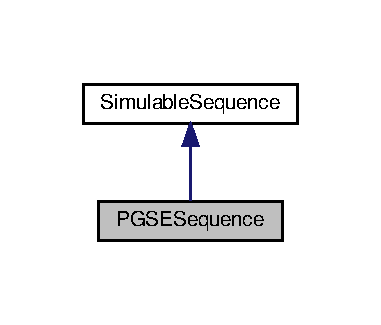
\includegraphics[width=183pt]{class_p_g_s_e_sequence__inherit__graph}
\end{center}
\end{figure}


Collaboration diagram for P\+G\+S\+E\+Sequence\+:\nopagebreak
\begin{figure}[H]
\begin{center}
\leavevmode
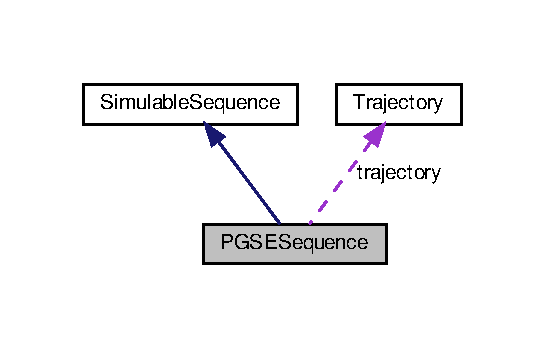
\includegraphics[width=262pt]{class_p_g_s_e_sequence__coll__graph}
\end{center}
\end{figure}
\subsection*{Public Member Functions}
\begin{DoxyCompactItemize}
\item 
\mbox{\Hypertarget{class_p_g_s_e_sequence_a29db64fbd60c54c191e8197e1818dce0}\label{class_p_g_s_e_sequence_a29db64fbd60c54c191e8197e1818dce0}} 
\hyperlink{class_p_g_s_e_sequence_a29db64fbd60c54c191e8197e1818dce0}{P\+G\+S\+E\+Sequence} ()
\begin{DoxyCompactList}\small\item\em Default constructor, set default N\+U\+LL values. Not to be used. \end{DoxyCompactList}\item 
\mbox{\Hypertarget{class_p_g_s_e_sequence_a31bcb2e91e27823bbe71904e180f7de9}\label{class_p_g_s_e_sequence_a31bcb2e91e27823bbe71904e180f7de9}} 
\hyperlink{class_p_g_s_e_sequence_a31bcb2e91e27823bbe71904e180f7de9}{P\+G\+S\+E\+Sequence} (\hyperlink{class_scheme}{Scheme} scheme\+\_\+)
\begin{DoxyCompactList}\small\item\em Main constructor. Takes a pre-\/loaded \hyperlink{class_scheme}{Scheme} file. \end{DoxyCompactList}\item 
\mbox{\Hypertarget{class_p_g_s_e_sequence_ab278a413c31a67f82712590897a556cb}\label{class_p_g_s_e_sequence_ab278a413c31a67f82712590897a556cb}} 
\hyperlink{class_p_g_s_e_sequence_ab278a413c31a67f82712590897a556cb}{P\+G\+S\+E\+Sequence} (\hyperlink{class_scheme}{Scheme} scheme\+\_\+, const char $\ast$traj\+\_\+file\+\_\+name)
\begin{DoxyCompactList}\small\item\em Main constructor. Takes a pre-\/loaded \hyperlink{class_scheme}{Scheme} file and a traj file name. if this argument is passed a traj file is should be written. \end{DoxyCompactList}\item 
\mbox{\Hypertarget{class_p_g_s_e_sequence_a262f1156c51983fba9b9a6b666dd2e07}\label{class_p_g_s_e_sequence_a262f1156c51983fba9b9a6b666dd2e07}} 
\hyperlink{class_p_g_s_e_sequence_a262f1156c51983fba9b9a6b666dd2e07}{P\+G\+S\+E\+Sequence} (const char $\ast$scheme\+\_\+file\+\_\+name)
\begin{DoxyCompactList}\small\item\em Constructor. Takes a the scheme file name to be loaded. \end{DoxyCompactList}\item 
\mbox{\Hypertarget{class_p_g_s_e_sequence_a1eb4e53eb0769b16eb9bb2156c769644}\label{class_p_g_s_e_sequence_a1eb4e53eb0769b16eb9bb2156c769644}} 
\hyperlink{class_p_g_s_e_sequence_a1eb4e53eb0769b16eb9bb2156c769644}{P\+G\+S\+E\+Sequence} (const char $\ast$scheme\+\_\+file\+\_\+name, const char $\ast$traj\+\_\+file\+\_\+name)
\begin{DoxyCompactList}\small\item\em Constructor. Takes a scheme file name to be loaded and atraj file name. if this argument is passed a traj file is should be written. \end{DoxyCompactList}\item 
\mbox{\Hypertarget{class_p_g_s_e_sequence_a7e5815e4ae0b3a6d42c45322fc69fdd6}\label{class_p_g_s_e_sequence_a7e5815e4ae0b3a6d42c45322fc69fdd6}} 
\hyperlink{class_p_g_s_e_sequence_a7e5815e4ae0b3a6d42c45322fc69fdd6}{$\sim$\+P\+G\+S\+E\+Sequence} ()
\begin{DoxyCompactList}\small\item\em Destuctor. Does nothing. \end{DoxyCompactList}\item 
\mbox{\Hypertarget{class_p_g_s_e_sequence_a3f2a705b7d3312944630f3d7f639e8e4}\label{class_p_g_s_e_sequence_a3f2a705b7d3312944630f3d7f639e8e4}} 
void \hyperlink{class_p_g_s_e_sequence_a3f2a705b7d3312944630f3d7f639e8e4}{get\+Grad\+Impulse} (int i, double t, double t\+Last, Eigen\+::\+Vector3d \&Gdt)
\begin{DoxyCompactList}\small\item\em For using w/o the adt array. \end{DoxyCompactList}\item 
\mbox{\Hypertarget{class_p_g_s_e_sequence_a9985ead781333f782d1dee54482eb0d2}\label{class_p_g_s_e_sequence_a9985ead781333f782d1dee54482eb0d2}} 
void \hyperlink{class_p_g_s_e_sequence_a9985ead781333f782d1dee54482eb0d2}{get\+Grad\+Impuse} (int i, double t, Eigen\+::\+Vector3d Gdt)
\begin{DoxyCompactList}\small\item\em For using with the adt array. \end{DoxyCompactList}\item 
\mbox{\Hypertarget{class_p_g_s_e_sequence_a8b0671a505f79a601d3d4d2d9b7f36cc}\label{class_p_g_s_e_sequence_a8b0671a505f79a601d3d4d2d9b7f36cc}} 
double \hyperlink{class_p_g_s_e_sequence_a8b0671a505f79a601d3d4d2d9b7f36cc}{getb\+Value} (unsigned)
\begin{DoxyCompactList}\small\item\em Analytical defined b-\/value. \end{DoxyCompactList}\item 
\mbox{\Hypertarget{class_p_g_s_e_sequence_a375c8a943f4857a323ffc404394b5d8a}\label{class_p_g_s_e_sequence_a375c8a943f4857a323ffc404394b5d8a}} 
double \hyperlink{class_p_g_s_e_sequence_a375c8a943f4857a323ffc404394b5d8a}{get\+Free\+Decay} (unsigned i, double D)
\begin{DoxyCompactList}\small\item\em Expected free Decay. \end{DoxyCompactList}\item 
double \hyperlink{class_p_g_s_e_sequence_a1373f02bffedb1e934818ae8d4fb8939}{get\+Numericalb\+Value} (unsigned)
\item 
\mbox{\Hypertarget{class_p_g_s_e_sequence_aec05e76b5c7b3361bd3e68301b262a0a}\label{class_p_g_s_e_sequence_aec05e76b5c7b3361bd3e68301b262a0a}} 
void \hyperlink{class_p_g_s_e_sequence_aec05e76b5c7b3361bd3e68301b262a0a}{get\+D\+W\+I\+Signal} ()
\begin{DoxyCompactList}\small\item\em Computes de DW signal from a trajfile. \end{DoxyCompactList}\item 
\mbox{\Hypertarget{class_p_g_s_e_sequence_a22005e67e3513690f9e46b1d531481b0}\label{class_p_g_s_e_sequence_a22005e67e3513690f9e46b1d531481b0}} 
void \hyperlink{class_p_g_s_e_sequence_a22005e67e3513690f9e46b1d531481b0}{read\+Scheme\+File} ()
\begin{DoxyCompactList}\small\item\em reads the scheme files \end{DoxyCompactList}\item 
virtual void \hyperlink{class_p_g_s_e_sequence_a6914efd208eab28a1ee6a3f28ca65478}{update\+\_\+phase\+\_\+shift} (double dt, double dt\+\_\+last, \hyperlink{class_walker}{Walker} walker)
\item 
\mbox{\Hypertarget{class_p_g_s_e_sequence_a850a2f22cdf8b420888cfa906e03e078}\label{class_p_g_s_e_sequence_a850a2f22cdf8b420888cfa906e03e078}} 
virtual void \hyperlink{class_p_g_s_e_sequence_a850a2f22cdf8b420888cfa906e03e078}{update\+\_\+phase\+\_\+shift} (double time\+\_\+step, Eigen\+::\+Matrix3\+Xd \hyperlink{class_p_g_s_e_sequence_a0fd0fb458384bfb65070fdab5165dde5}{trajectory})
\begin{DoxyCompactList}\small\item\em Updates the phase shift using the full stored trajectory. \end{DoxyCompactList}\item 
\mbox{\Hypertarget{class_p_g_s_e_sequence_ae2b79f12ccd2f2446a498cb51f45e88d}\label{class_p_g_s_e_sequence_ae2b79f12ccd2f2446a498cb51f45e88d}} 
virtual void \hyperlink{class_p_g_s_e_sequence_ae2b79f12ccd2f2446a498cb51f45e88d}{update\+\_\+\+D\+W\+I\+\_\+signal} (\hyperlink{class_walker}{Walker} \&walker)
\begin{DoxyCompactList}\small\item\em Updates the D\+WI signal using the cumulated phase shift. \end{DoxyCompactList}\item 
\mbox{\Hypertarget{class_p_g_s_e_sequence_a885a0415519683a7fbfa1883f7f3d807}\label{class_p_g_s_e_sequence_a885a0415519683a7fbfa1883f7f3d807}} 
double \hyperlink{class_p_g_s_e_sequence_a885a0415519683a7fbfa1883f7f3d807}{get\+\_\+adt} (int grad\+\_\+index, double t, double t\+Last)
\begin{DoxyCompactList}\small\item\em computes de signal value and sign in a certain time step. \end{DoxyCompactList}\item 
\mbox{\Hypertarget{class_p_g_s_e_sequence_afa9e363ef76474d5e2495407034a10d4}\label{class_p_g_s_e_sequence_afa9e363ef76474d5e2495407034a10d4}} 
double \hyperlink{class_p_g_s_e_sequence_afa9e363ef76474d5e2495407034a10d4}{print\+\_\+adt\+\_\+and\+\_\+dt} (int grad\+\_\+index, double t, double t\+Last)
\begin{DoxyCompactList}\small\item\em prints the array adt in the format (). \end{DoxyCompactList}\item 
\mbox{\Hypertarget{class_p_g_s_e_sequence_a89f9bf116876b04403058a240a91efa3}\label{class_p_g_s_e_sequence_a89f9bf116876b04403058a240a91efa3}} 
virtual void \hyperlink{class_p_g_s_e_sequence_a89f9bf116876b04403058a240a91efa3}{set\+Number\+Of\+Steps} (unsigned \hyperlink{class_p_g_s_e_sequence_a07e27e6e8a8506521386a291d62e8423}{T})
\begin{DoxyCompactList}\small\item\em Set the number of time steps if they are known. \end{DoxyCompactList}\item 
\mbox{\Hypertarget{class_p_g_s_e_sequence_ac115d93aabb283f19568f55493d57ded}\label{class_p_g_s_e_sequence_ac115d93aabb283f19568f55493d57ded}} 
virtual void \hyperlink{class_p_g_s_e_sequence_ac115d93aabb283f19568f55493d57ded}{compute\+Dynamic\+Time\+Steps} ()
\begin{DoxyCompactList}\small\item\em Compute the time for all the steps when they are not constant. \end{DoxyCompactList}\end{DoxyCompactItemize}
\subsection*{Public Attributes}
\begin{DoxyCompactItemize}
\item 
double \hyperlink{class_p_g_s_e_sequence_a06df939859fd2ed6104bfee584f893a1}{TE}
\item 
int \hyperlink{class_p_g_s_e_sequence_a07e27e6e8a8506521386a291d62e8423}{T}
\item 
double \hyperlink{class_p_g_s_e_sequence_a0c7e884c3b71cbcc04d6cb2d5f2a5eb9}{dyn\+\_\+duration}
\item 
std\+::vector$<$ std\+::vector$<$ double $>$ $>$ \hyperlink{class_p_g_s_e_sequence_a7349d86720a34e75eaf578fdfd3caeeb}{scheme}
\item 
\hyperlink{class_trajectory}{Trajectory} \hyperlink{class_p_g_s_e_sequence_a0fd0fb458384bfb65070fdab5165dde5}{trajectory}
\end{DoxyCompactItemize}


\subsection{Member Function Documentation}
\mbox{\Hypertarget{class_p_g_s_e_sequence_a1373f02bffedb1e934818ae8d4fb8939}\label{class_p_g_s_e_sequence_a1373f02bffedb1e934818ae8d4fb8939}} 
\index{P\+G\+S\+E\+Sequence@{P\+G\+S\+E\+Sequence}!get\+Numericalb\+Value@{get\+Numericalb\+Value}}
\index{get\+Numericalb\+Value@{get\+Numericalb\+Value}!P\+G\+S\+E\+Sequence@{P\+G\+S\+E\+Sequence}}
\subsubsection{\texorpdfstring{get\+Numericalb\+Value()}{getNumericalbValue()}}
{\footnotesize\ttfamily double P\+G\+S\+E\+Sequence\+::get\+Numericalb\+Value (\begin{DoxyParamCaption}\item[{unsigned}]{i }\end{DoxyParamCaption})}

\begin{DoxyWarning}{Warning}
not implemented yet. 
\end{DoxyWarning}
\mbox{\Hypertarget{class_p_g_s_e_sequence_a6914efd208eab28a1ee6a3f28ca65478}\label{class_p_g_s_e_sequence_a6914efd208eab28a1ee6a3f28ca65478}} 
\index{P\+G\+S\+E\+Sequence@{P\+G\+S\+E\+Sequence}!update\+\_\+phase\+\_\+shift@{update\+\_\+phase\+\_\+shift}}
\index{update\+\_\+phase\+\_\+shift@{update\+\_\+phase\+\_\+shift}!P\+G\+S\+E\+Sequence@{P\+G\+S\+E\+Sequence}}
\subsubsection{\texorpdfstring{update\+\_\+phase\+\_\+shift()}{update\_phase\_shift()}}
{\footnotesize\ttfamily void P\+G\+S\+E\+Sequence\+::update\+\_\+phase\+\_\+shift (\begin{DoxyParamCaption}\item[{double}]{dt,  }\item[{double}]{dt\+\_\+last,  }\item[{\hyperlink{class_walker}{Walker}}]{walker }\end{DoxyParamCaption})\hspace{0.3cm}{\ttfamily [virtual]}}


\begin{DoxyParams}{Parameters}
{\em i} & updated walker \\
\hline
\end{DoxyParams}


Implements \hyperlink{class_simulable_sequence_ad7b2a30f563343aa65489aa553d4df63}{Simulable\+Sequence}.



\subsection{Member Data Documentation}
\mbox{\Hypertarget{class_p_g_s_e_sequence_a0c7e884c3b71cbcc04d6cb2d5f2a5eb9}\label{class_p_g_s_e_sequence_a0c7e884c3b71cbcc04d6cb2d5f2a5eb9}} 
\index{P\+G\+S\+E\+Sequence@{P\+G\+S\+E\+Sequence}!dyn\+\_\+duration@{dyn\+\_\+duration}}
\index{dyn\+\_\+duration@{dyn\+\_\+duration}!P\+G\+S\+E\+Sequence@{P\+G\+S\+E\+Sequence}}
\subsubsection{\texorpdfstring{dyn\+\_\+duration}{dyn\_duration}}
{\footnotesize\ttfamily double P\+G\+S\+E\+Sequence\+::dyn\+\_\+duration}

simulation duration (miliseconds) \mbox{\Hypertarget{class_p_g_s_e_sequence_a7349d86720a34e75eaf578fdfd3caeeb}\label{class_p_g_s_e_sequence_a7349d86720a34e75eaf578fdfd3caeeb}} 
\index{P\+G\+S\+E\+Sequence@{P\+G\+S\+E\+Sequence}!scheme@{scheme}}
\index{scheme@{scheme}!P\+G\+S\+E\+Sequence@{P\+G\+S\+E\+Sequence}}
\subsubsection{\texorpdfstring{scheme}{scheme}}
{\footnotesize\ttfamily std\+::vector$<$ std\+::vector$<$double$>$ $>$ P\+G\+S\+E\+Sequence\+::scheme}

\hyperlink{class_scheme}{Scheme} file values \mbox{\Hypertarget{class_p_g_s_e_sequence_a07e27e6e8a8506521386a291d62e8423}\label{class_p_g_s_e_sequence_a07e27e6e8a8506521386a291d62e8423}} 
\index{P\+G\+S\+E\+Sequence@{P\+G\+S\+E\+Sequence}!T@{T}}
\index{T@{T}!P\+G\+S\+E\+Sequence@{P\+G\+S\+E\+Sequence}}
\subsubsection{\texorpdfstring{T}{T}}
{\footnotesize\ttfamily int P\+G\+S\+E\+Sequence\+::T}

num bins (time steps) \mbox{\Hypertarget{class_p_g_s_e_sequence_a06df939859fd2ed6104bfee584f893a1}\label{class_p_g_s_e_sequence_a06df939859fd2ed6104bfee584f893a1}} 
\index{P\+G\+S\+E\+Sequence@{P\+G\+S\+E\+Sequence}!TE@{TE}}
\index{TE@{TE}!P\+G\+S\+E\+Sequence@{P\+G\+S\+E\+Sequence}}
\subsubsection{\texorpdfstring{TE}{TE}}
{\footnotesize\ttfamily double P\+G\+S\+E\+Sequence\+::\+TE}

Time Echo. \mbox{\Hypertarget{class_p_g_s_e_sequence_a0fd0fb458384bfb65070fdab5165dde5}\label{class_p_g_s_e_sequence_a0fd0fb458384bfb65070fdab5165dde5}} 
\index{P\+G\+S\+E\+Sequence@{P\+G\+S\+E\+Sequence}!trajectory@{trajectory}}
\index{trajectory@{trajectory}!P\+G\+S\+E\+Sequence@{P\+G\+S\+E\+Sequence}}
\subsubsection{\texorpdfstring{trajectory}{trajectory}}
{\footnotesize\ttfamily \hyperlink{class_trajectory}{Trajectory} P\+G\+S\+E\+Sequence\+::trajectory}

If the signal is computed from a .trajfile 

The documentation for this class was generated from the following files\+:\begin{DoxyCompactItemize}
\item 
src/pgsesequence.\+h\item 
src/pgsesequence.\+cpp\end{DoxyCompactItemize}

\hypertarget{class_plane}{}\section{Plane Class Reference}
\label{class_plane}\index{Plane@{Plane}}


Main class. Implements basic voxel limits and operations. =================================================/.  




{\ttfamily \#include $<$voxel.\+h$>$}

\subsection*{Public Member Functions}
\begin{DoxyCompactItemize}
\item 
\mbox{\Hypertarget{class_plane_a8b1516b02b3ab4bdfe48234db82da168}\label{class_plane_a8b1516b02b3ab4bdfe48234db82da168}} 
{\bfseries Plane} (Eigen\+::\+Vector3d normal\+\_\+, Eigen\+::\+Vector3d plane\+\_\+center\+\_\+, double d\+\_\+)
\item 
\mbox{\Hypertarget{class_plane_a942208920a6e4762e3dc9aab76305667}\label{class_plane_a942208920a6e4762e3dc9aab76305667}} 
{\bfseries Plane} (Eigen\+::\+Vector3d \&a, Eigen\+::\+Vector3d \&b, Eigen\+::\+Vector3d \&c, Eigen\+::\+Vector3d \&d)
\item 
\mbox{\Hypertarget{class_plane_a1a4e24c5ca029ceb787f291a11adac8f}\label{class_plane_a1a4e24c5ca029ceb787f291a11adac8f}} 
bool {\bfseries Check\+Collision} (\hyperlink{class_walker}{Walker} \&walker, Eigen\+::\+Vector3d \&step, double tmax, \hyperlink{class_collision}{Collision} \&colision)
\end{DoxyCompactItemize}
\subsection*{Public Attributes}
\begin{DoxyCompactItemize}
\item 
\mbox{\Hypertarget{class_plane_a229ee65fd1663c7e7bd101309ddcf5e0}\label{class_plane_a229ee65fd1663c7e7bd101309ddcf5e0}} 
Eigen\+::\+Vector3d {\bfseries normal}
\item 
\mbox{\Hypertarget{class_plane_a20cfe0415a4f25f03d2d639ae9a647e9}\label{class_plane_a20cfe0415a4f25f03d2d639ae9a647e9}} 
Eigen\+::\+Vector3d {\bfseries plane\+\_\+center}
\item 
\mbox{\Hypertarget{class_plane_a13e69abc574bead3f8f450bbe2b43cf9}\label{class_plane_a13e69abc574bead3f8f450bbe2b43cf9}} 
double {\bfseries d}
\end{DoxyCompactItemize}


\subsection{Detailed Description}
Main class. Implements basic voxel limits and operations. =================================================/. 

Class to handle and manage the voxels in the simulations. So far only one voxel at the time can be handled. To improve to several voxels, modifications shall be done.

\begin{DoxyAuthor}{Author}
Jonathan Rafael 
\end{DoxyAuthor}
\begin{DoxyDate}{Date}
July 2016 
\end{DoxyDate}
\begin{DoxyVersion}{Version}
0.\+2 =============================================================================================================+
\end{DoxyVersion}
Auxiliary class to implements plane\textquotesingle{}s interactions with particles. 

The documentation for this class was generated from the following files\+:\begin{DoxyCompactItemize}
\item 
src/voxel.\+h\item 
src/voxel.\+cpp\end{DoxyCompactItemize}

\hypertarget{class_p_l_y_collision_sphere}{}\section{P\+L\+Y\+Collision\+Sphere Class Reference}
\label{class_p_l_y_collision_sphere}\index{P\+L\+Y\+Collision\+Sphere@{P\+L\+Y\+Collision\+Sphere}}


Inheritance diagram for P\+L\+Y\+Collision\+Sphere\+:
\nopagebreak
\begin{figure}[H]
\begin{center}
\leavevmode
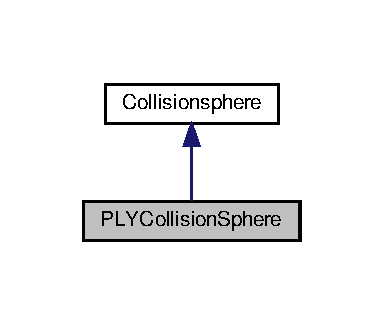
\includegraphics[width=184pt]{class_p_l_y_collision_sphere__inherit__graph}
\end{center}
\end{figure}


Collaboration diagram for P\+L\+Y\+Collision\+Sphere\+:
\nopagebreak
\begin{figure}[H]
\begin{center}
\leavevmode
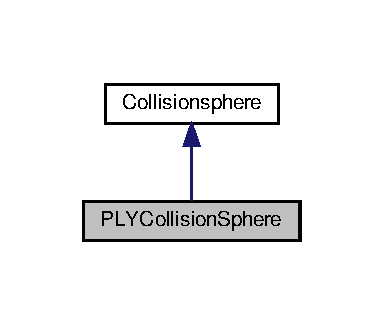
\includegraphics[width=184pt]{class_p_l_y_collision_sphere__coll__graph}
\end{center}
\end{figure}
\subsection*{Public Member Functions}
\begin{DoxyCompactItemize}
\item 
void \hyperlink{class_p_l_y_collision_sphere_adc8f318a913935cdd31d81f1c96192eb}{pop\+From\+Small\+Sphere} (unsigned i, unsigned t)
\begin{DoxyCompactList}\small\item\em This function receives a index from the collision list and moves the value to the last position of the list. then decrease the inner sphere end index. This way this index is no longer considered inner collision list. \end{DoxyCompactList}\item 
void \hyperlink{class_p_l_y_collision_sphere_a546ea2c6fe80908502fba0350c4f9726}{push\+To\+Small\+Sphere} (unsigned i, unsigned t)
\begin{DoxyCompactList}\small\item\em This function receives a index from the collision list and moves the value to the last position of the list. then increse the inner sphere end index. This way this index is now included in the inner collision list. \end{DoxyCompactList}\item 
\mbox{\Hypertarget{class_p_l_y_collision_sphere_ac9cf3838088310db3dc8f0d282c3c383}\label{class_p_l_y_collision_sphere_ac9cf3838088310db3dc8f0d282c3c383}} 
void \hyperlink{class_p_l_y_collision_sphere_ac9cf3838088310db3dc8f0d282c3c383}{pop\+From\+Big\+Sphere} (unsigned i, unsigned t)
\begin{DoxyCompactList}\small\item\em This function receives a index from the collision list and moves the value to the last position of the list. Then decrease the inner sphere end index. This way this index is now excluded in the outer collision list. \end{DoxyCompactList}\item 
\mbox{\Hypertarget{class_p_l_y_collision_sphere_aa1fe5971687051f0de78a12ee4b31574}\label{class_p_l_y_collision_sphere_aa1fe5971687051f0de78a12ee4b31574}} 
void \hyperlink{class_p_l_y_collision_sphere_aa1fe5971687051f0de78a12ee4b31574}{push\+To\+Big\+Sphere} (unsigned i, unsigned t)
\begin{DoxyCompactList}\small\item\em This function receives a index from the collision list and moves the value to the last position of the list. Then increase the inner sphere end index. This way this index is now included in the outer collision list. \end{DoxyCompactList}\item 
void \hyperlink{class_p_l_y_collision_sphere_acf52aecaf0bf676087035151e6c662c9}{set\+Big\+Sphere\+Size} (float size)
\item 
void \hyperlink{class_p_l_y_collision_sphere_af9ba1a8616bb5703e58f392f45c6c069}{set\+Small\+Sphere\+Size} (float size)
\item 
void \hyperlink{class_p_l_y_collision_sphere_a10e46dea74b839faf34872028eafae46}{push\+\_\+ply} (std\+::vector$<$ unsigned $>$ list)
\end{DoxyCompactItemize}
\subsection*{Public Attributes}
\begin{DoxyCompactItemize}
\item 
std\+::vector$<$ unsigned $>$ \hyperlink{class_p_l_y_collision_sphere_a7fd18a4a8a9dbb2f7104f9b9a5dd6766}{small\+\_\+sphere\+\_\+list\+\_\+end}
\item 
std\+::vector$<$ unsigned $>$ \hyperlink{class_p_l_y_collision_sphere_aadf7b345b8c91791fa96e00862bc8cbb}{big\+\_\+sphere\+\_\+list\+\_\+end}
\item 
std\+::vector$<$ std\+::vector$<$ unsigned $>$ $>$ $\ast$ \hyperlink{class_p_l_y_collision_sphere_a6ef04af98385142ed0b41a2e35f423b9}{collision\+\_\+list}
\end{DoxyCompactItemize}


\subsection{Member Function Documentation}
\mbox{\Hypertarget{class_p_l_y_collision_sphere_adc8f318a913935cdd31d81f1c96192eb}\label{class_p_l_y_collision_sphere_adc8f318a913935cdd31d81f1c96192eb}} 
\index{P\+L\+Y\+Collision\+Sphere@{P\+L\+Y\+Collision\+Sphere}!pop\+From\+Small\+Sphere@{pop\+From\+Small\+Sphere}}
\index{pop\+From\+Small\+Sphere@{pop\+From\+Small\+Sphere}!P\+L\+Y\+Collision\+Sphere@{P\+L\+Y\+Collision\+Sphere}}
\subsubsection{\texorpdfstring{pop\+From\+Small\+Sphere()}{popFromSmallSphere()}}
{\footnotesize\ttfamily void P\+L\+Y\+Collision\+Sphere\+::pop\+From\+Small\+Sphere (\begin{DoxyParamCaption}\item[{unsigned}]{i,  }\item[{unsigned}]{t }\end{DoxyParamCaption})}



This function receives a index from the collision list and moves the value to the last position of the list. then decrease the inner sphere end index. This way this index is no longer considered inner collision list. 

Removes one index from the list by moving it to the end of the list and decreading the index. \mbox{\Hypertarget{class_p_l_y_collision_sphere_a10e46dea74b839faf34872028eafae46}\label{class_p_l_y_collision_sphere_a10e46dea74b839faf34872028eafae46}} 
\index{P\+L\+Y\+Collision\+Sphere@{P\+L\+Y\+Collision\+Sphere}!push\+\_\+ply@{push\+\_\+ply}}
\index{push\+\_\+ply@{push\+\_\+ply}!P\+L\+Y\+Collision\+Sphere@{P\+L\+Y\+Collision\+Sphere}}
\subsubsection{\texorpdfstring{push\+\_\+ply()}{push\_ply()}}
{\footnotesize\ttfamily void P\+L\+Y\+Collision\+Sphere\+::push\+\_\+ply (\begin{DoxyParamCaption}\item[{std\+::vector$<$ unsigned $>$}]{list }\end{DoxyParamCaption})}


\begin{DoxyParams}{Parameters}
{\em element} & value to be added to the obstacle list \\
\hline
\end{DoxyParams}
\mbox{\Hypertarget{class_p_l_y_collision_sphere_a546ea2c6fe80908502fba0350c4f9726}\label{class_p_l_y_collision_sphere_a546ea2c6fe80908502fba0350c4f9726}} 
\index{P\+L\+Y\+Collision\+Sphere@{P\+L\+Y\+Collision\+Sphere}!push\+To\+Small\+Sphere@{push\+To\+Small\+Sphere}}
\index{push\+To\+Small\+Sphere@{push\+To\+Small\+Sphere}!P\+L\+Y\+Collision\+Sphere@{P\+L\+Y\+Collision\+Sphere}}
\subsubsection{\texorpdfstring{push\+To\+Small\+Sphere()}{pushToSmallSphere()}}
{\footnotesize\ttfamily void P\+L\+Y\+Collision\+Sphere\+::push\+To\+Small\+Sphere (\begin{DoxyParamCaption}\item[{unsigned}]{i,  }\item[{unsigned}]{t }\end{DoxyParamCaption})}



This function receives a index from the collision list and moves the value to the last position of the list. then increse the inner sphere end index. This way this index is now included in the inner collision list. 

Adds one element to the list by moving it in front of the current index and increasing the index. \mbox{\Hypertarget{class_p_l_y_collision_sphere_acf52aecaf0bf676087035151e6c662c9}\label{class_p_l_y_collision_sphere_acf52aecaf0bf676087035151e6c662c9}} 
\index{P\+L\+Y\+Collision\+Sphere@{P\+L\+Y\+Collision\+Sphere}!set\+Big\+Sphere\+Size@{set\+Big\+Sphere\+Size}}
\index{set\+Big\+Sphere\+Size@{set\+Big\+Sphere\+Size}!P\+L\+Y\+Collision\+Sphere@{P\+L\+Y\+Collision\+Sphere}}
\subsubsection{\texorpdfstring{set\+Big\+Sphere\+Size()}{setBigSphereSize()}}
{\footnotesize\ttfamily void P\+L\+Y\+Collision\+Sphere\+::set\+Big\+Sphere\+Size (\begin{DoxyParamCaption}\item[{float}]{size }\end{DoxyParamCaption})}


\begin{DoxyParams}{Parameters}
{\em size} & of the list \\
\hline
\end{DoxyParams}
\mbox{\Hypertarget{class_p_l_y_collision_sphere_af9ba1a8616bb5703e58f392f45c6c069}\label{class_p_l_y_collision_sphere_af9ba1a8616bb5703e58f392f45c6c069}} 
\index{P\+L\+Y\+Collision\+Sphere@{P\+L\+Y\+Collision\+Sphere}!set\+Small\+Sphere\+Size@{set\+Small\+Sphere\+Size}}
\index{set\+Small\+Sphere\+Size@{set\+Small\+Sphere\+Size}!P\+L\+Y\+Collision\+Sphere@{P\+L\+Y\+Collision\+Sphere}}
\subsubsection{\texorpdfstring{set\+Small\+Sphere\+Size()}{setSmallSphereSize()}}
{\footnotesize\ttfamily void P\+L\+Y\+Collision\+Sphere\+::set\+Small\+Sphere\+Size (\begin{DoxyParamCaption}\item[{float}]{size }\end{DoxyParamCaption})}


\begin{DoxyParams}{Parameters}
{\em size} & of the list \\
\hline
\end{DoxyParams}


\subsection{Member Data Documentation}
\mbox{\Hypertarget{class_p_l_y_collision_sphere_aadf7b345b8c91791fa96e00862bc8cbb}\label{class_p_l_y_collision_sphere_aadf7b345b8c91791fa96e00862bc8cbb}} 
\index{P\+L\+Y\+Collision\+Sphere@{P\+L\+Y\+Collision\+Sphere}!big\+\_\+sphere\+\_\+list\+\_\+end@{big\+\_\+sphere\+\_\+list\+\_\+end}}
\index{big\+\_\+sphere\+\_\+list\+\_\+end@{big\+\_\+sphere\+\_\+list\+\_\+end}!P\+L\+Y\+Collision\+Sphere@{P\+L\+Y\+Collision\+Sphere}}
\subsubsection{\texorpdfstring{big\+\_\+sphere\+\_\+list\+\_\+end}{big\_sphere\_list\_end}}
{\footnotesize\ttfamily std\+::vector$<$unsigned$>$ P\+L\+Y\+Collision\+Sphere\+::big\+\_\+sphere\+\_\+list\+\_\+end}

Index vecotr of the L\+A\+ST element on the list for the big collision sphere \mbox{\Hypertarget{class_p_l_y_collision_sphere_a6ef04af98385142ed0b41a2e35f423b9}\label{class_p_l_y_collision_sphere_a6ef04af98385142ed0b41a2e35f423b9}} 
\index{P\+L\+Y\+Collision\+Sphere@{P\+L\+Y\+Collision\+Sphere}!collision\+\_\+list@{collision\+\_\+list}}
\index{collision\+\_\+list@{collision\+\_\+list}!P\+L\+Y\+Collision\+Sphere@{P\+L\+Y\+Collision\+Sphere}}
\subsubsection{\texorpdfstring{collision\+\_\+list}{collision\_list}}
{\footnotesize\ttfamily std\+::vector$<$std\+::vector$<$unsigned$>$ $>$$\ast$ P\+L\+Y\+Collision\+Sphere\+::collision\+\_\+list}

Pointer to the list with the triangle indexes for each P\+LY. The indexes are permuted in its position. \mbox{\Hypertarget{class_p_l_y_collision_sphere_a7fd18a4a8a9dbb2f7104f9b9a5dd6766}\label{class_p_l_y_collision_sphere_a7fd18a4a8a9dbb2f7104f9b9a5dd6766}} 
\index{P\+L\+Y\+Collision\+Sphere@{P\+L\+Y\+Collision\+Sphere}!small\+\_\+sphere\+\_\+list\+\_\+end@{small\+\_\+sphere\+\_\+list\+\_\+end}}
\index{small\+\_\+sphere\+\_\+list\+\_\+end@{small\+\_\+sphere\+\_\+list\+\_\+end}!P\+L\+Y\+Collision\+Sphere@{P\+L\+Y\+Collision\+Sphere}}
\subsubsection{\texorpdfstring{small\+\_\+sphere\+\_\+list\+\_\+end}{small\_sphere\_list\_end}}
{\footnotesize\ttfamily std\+::vector$<$unsigned$>$ P\+L\+Y\+Collision\+Sphere\+::small\+\_\+sphere\+\_\+list\+\_\+end}

Index vector of the L\+A\+ST element on the list for the small collision sphere 

The documentation for this class was generated from the following files\+:\begin{DoxyCompactItemize}
\item 
src/collisionsphere.\+h\item 
src/collisionsphere.\+cpp\end{DoxyCompactItemize}

\hypertarget{class_p_l_y_obstacle}{}\section{P\+L\+Y\+Obstacle Class Reference}
\label{class_p_l_y_obstacle}\index{P\+L\+Y\+Obstacle@{P\+L\+Y\+Obstacle}}


Ply\+Obstacle Derived Class ====================================================================/.  




{\ttfamily \#include $<$plyobstacle.\+h$>$}



Inheritance diagram for P\+L\+Y\+Obstacle\+:
\nopagebreak
\begin{figure}[H]
\begin{center}
\leavevmode
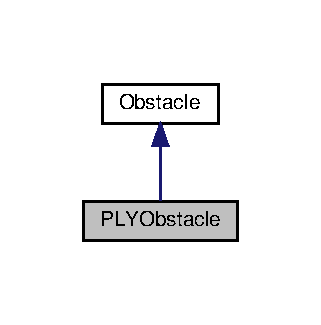
\includegraphics[width=154pt]{class_p_l_y_obstacle__inherit__graph}
\end{center}
\end{figure}


Collaboration diagram for P\+L\+Y\+Obstacle\+:
\nopagebreak
\begin{figure}[H]
\begin{center}
\leavevmode
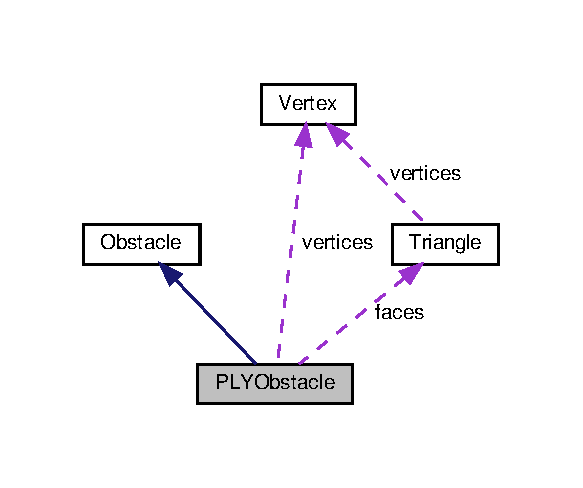
\includegraphics[width=280pt]{class_p_l_y_obstacle__coll__graph}
\end{center}
\end{figure}
\subsection*{Public Member Functions}
\begin{DoxyCompactItemize}
\item 
\mbox{\Hypertarget{class_p_l_y_obstacle_a8995508a44982787e9aa44bc8d47f669}\label{class_p_l_y_obstacle_a8995508a44982787e9aa44bc8d47f669}} 
{\bfseries P\+L\+Y\+Obstacle} (std\+::string path, double scale\+\_\+factor\+\_\+=1)
\item 
\mbox{\Hypertarget{class_p_l_y_obstacle_a52649eb1362242e7681e75f7409ee940}\label{class_p_l_y_obstacle_a52649eb1362242e7681e75f7409ee940}} 
{\bfseries P\+L\+Y\+Obstacle} (std\+::string path, std\+::vector$<$ Eigen\+::\+Vector3d $>$ \&centers, double max\+\_\+distance=I\+N\+F\+I\+N\+I\+TY, double scale\+\_\+factor\+\_\+=1)
\item 
\mbox{\Hypertarget{class_p_l_y_obstacle_a4e409be3ded2cb3fe2f3cae97fafd266}\label{class_p_l_y_obstacle_a4e409be3ded2cb3fe2f3cae97fafd266}} 
void {\bfseries read\+P\+L\+Y\+\_\+\+A\+S\+C\+I\+I\+\_\+triangle\+Fan} (std\+::string ply\+\_\+file)
\item 
\mbox{\Hypertarget{class_p_l_y_obstacle_af5db9263d9555682f8345cef2d116eb4}\label{class_p_l_y_obstacle_af5db9263d9555682f8345cef2d116eb4}} 
void {\bfseries read\+P\+L\+Y\+\_\+\+A\+S\+C\+I\+I\+\_\+triangles} (std\+::string ply\+\_\+file)
\item 
\mbox{\Hypertarget{class_p_l_y_obstacle_a428018f72231740be297c9cd24752bbd}\label{class_p_l_y_obstacle_a428018f72231740be297c9cd24752bbd}} 
void {\bfseries read\+P\+L\+Y\+\_\+\+A\+S\+C\+I\+I\+\_\+triangles\+Subdivition\+Distance} (std\+::string ply\+\_\+file, std\+::vector$<$ Eigen\+::\+Vector3d $>$ \&centers, double max\+\_\+distance)
\item 
\mbox{\Hypertarget{class_p_l_y_obstacle_ad0ce0257b8250a5e325da3f0d58e90de}\label{class_p_l_y_obstacle_ad0ce0257b8250a5e325da3f0d58e90de}} 
void {\bfseries set\+Scale\+Factor} (double scale)
\item 
\mbox{\Hypertarget{class_p_l_y_obstacle_aa43eb5a352acb2305b0ad5d4f3535dd1}\label{class_p_l_y_obstacle_aa43eb5a352acb2305b0ad5d4f3535dd1}} 
bool {\bfseries check\+Collision} (\hyperlink{class_walker}{Walker} \&walker, Eigen\+::\+Vector3d \&step, double \&step\+\_\+lenght, \hyperlink{class_collision}{Collision} \&colision)
\item 
\mbox{\Hypertarget{class_p_l_y_obstacle_ada5a479826a277b78f7531693809e69c}\label{class_p_l_y_obstacle_ada5a479826a277b78f7531693809e69c}} 
bool {\bfseries check\+Collision} (\hyperlink{class_walker}{Walker} \&walker, Eigen\+::\+Vector3d \&step, double \&step\+\_\+lenght, \hyperlink{class_collision}{Collision} \&colision, std\+::vector$<$ unsigned $>$ \&triangle\+\_\+list, unsigned list\+\_\+end)
\item 
\mbox{\Hypertarget{class_p_l_y_obstacle_aef64d5d9c5ea9d16c0efb75b89dc7ba0}\label{class_p_l_y_obstacle_aef64d5d9c5ea9d16c0efb75b89dc7ba0}} 
double {\bfseries min\+Distance} (\hyperlink{class_walker}{Walker} \&w, unsigned t)
\end{DoxyCompactItemize}
\subsection*{Public Attributes}
\begin{DoxyCompactItemize}
\item 
\mbox{\Hypertarget{class_p_l_y_obstacle_a5e14e62690601a6273147aca53751569}\label{class_p_l_y_obstacle_a5e14e62690601a6273147aca53751569}} 
unsigned {\bfseries vert\+\_\+number}
\item 
\mbox{\Hypertarget{class_p_l_y_obstacle_a9664285e5921c10b8d05954849f23e8d}\label{class_p_l_y_obstacle_a9664285e5921c10b8d05954849f23e8d}} 
unsigned {\bfseries face\+\_\+number}
\item 
\mbox{\Hypertarget{class_p_l_y_obstacle_ab384ad44fb6165d7d7277157e774ba40}\label{class_p_l_y_obstacle_ab384ad44fb6165d7d7277157e774ba40}} 
std\+::string {\bfseries file\+\_\+path}
\item 
\mbox{\Hypertarget{class_p_l_y_obstacle_a59d10b1c902e053caaf905e81bb618a6}\label{class_p_l_y_obstacle_a59d10b1c902e053caaf905e81bb618a6}} 
\hyperlink{class_vertex}{Vertex} $\ast$ {\bfseries vertices}
\item 
\mbox{\Hypertarget{class_p_l_y_obstacle_acd5752df4a98fbe92382184d732ddbc9}\label{class_p_l_y_obstacle_acd5752df4a98fbe92382184d732ddbc9}} 
\hyperlink{class_triangle}{Triangle} $\ast$ {\bfseries faces}
\item 
\mbox{\Hypertarget{class_p_l_y_obstacle_a3ddffa50af76259975a4b8d13c1019da}\label{class_p_l_y_obstacle_a3ddffa50af76259975a4b8d13c1019da}} 
double {\bfseries scale\+\_\+factor}
\item 
\mbox{\Hypertarget{class_p_l_y_obstacle_acf5a992f0da5e81dddf32484e24956ac}\label{class_p_l_y_obstacle_acf5a992f0da5e81dddf32484e24956ac}} 
int {\bfseries id}
\end{DoxyCompactItemize}


\subsection{Detailed Description}
Ply\+Obstacle Derived Class ====================================================================/. 

\hyperlink{class_p_l_y_obstacle}{P\+L\+Y\+Obstacle} derived class. Implements obstacles loaded from pre-\/defined PY meshes. \begin{DoxyAuthor}{Author}
Jonathan Rafael 
\end{DoxyAuthor}
\begin{DoxyDate}{Date}
November 2016 \subsection*{0.\+2 }
\end{DoxyDate}


Implements obstacles loaded from pre-\/constructed P\+LY meshes. The P\+LY format should be without any other experiment. 

The documentation for this class was generated from the following files\+:\begin{DoxyCompactItemize}
\item 
src/plyobstacle.\+h\item 
src/plyobstacle.\+cpp\end{DoxyCompactItemize}

\hypertarget{class_propagator}{}\section{Propagator Class Reference}
\label{class_propagator}\index{Propagator@{Propagator}}
\subsection*{Public Member Functions}
\begin{DoxyCompactItemize}
\item 
\mbox{\Hypertarget{class_propagator_aadc489a4d28c7a91e092fb7cef3b7a62}\label{class_propagator_aadc489a4d28c7a91e092fb7cef3b7a62}} 
void {\bfseries init\+Propagator} ()
\end{DoxyCompactItemize}
\subsection*{Public Attributes}
\begin{DoxyCompactItemize}
\item 
\mbox{\Hypertarget{class_propagator_a77f3732528ba16cef0092bc03a9d3020}\label{class_propagator_a77f3732528ba16cef0092bc03a9d3020}} 
uint {\bfseries num\+\_\+dirs} =0
\item 
\mbox{\Hypertarget{class_propagator_ab2e3c09934290a84abd3726faadbadc3}\label{class_propagator_ab2e3c09934290a84abd3726faadbadc3}} 
uint {\bfseries num\+\_\+times} = 0
\item 
\mbox{\Hypertarget{class_propagator_a2adc46036a2a2a8417ccdcd57e0c5f55}\label{class_propagator_a2adc46036a2a2a8417ccdcd57e0c5f55}} 
Eigen\+::\+Matrix3\+Xf {\bfseries directions}
\item 
\mbox{\Hypertarget{class_propagator_a9908ca97eaa8011f368510bc8ecc2343}\label{class_propagator_a9908ca97eaa8011f368510bc8ecc2343}} 
std\+::vector$<$ unsigned $>$ {\bfseries log\+\_\+times}
\item 
\mbox{\Hypertarget{class_propagator_aac52b49320c34b14b8bb8c5186f16bab}\label{class_propagator_aac52b49320c34b14b8bb8c5186f16bab}} 
std\+::vector$<$ std\+::vector$<$ float $>$ $>$ {\bfseries propagator\+\_\+log}
\end{DoxyCompactItemize}


The documentation for this class was generated from the following files\+:\begin{DoxyCompactItemize}
\item 
src/propagator.\+h\item 
src/propagator.\+cpp\end{DoxyCompactItemize}

\hypertarget{class_scheme}{}\section{Scheme Class Reference}
\label{class_scheme}\index{Scheme@{Scheme}}


Auxiliary class to save scheme\+\_\+files values =============================================================/.  




{\ttfamily \#include $<$scheme.\+h$>$}

\subsection*{Public Member Functions}
\begin{DoxyCompactItemize}
\item 
\mbox{\Hypertarget{class_scheme_a932eafa378988202a457037db3846aac}\label{class_scheme_a932eafa378988202a457037db3846aac}} 
{\bfseries Scheme} (std\+::string scheme\+\_\+file\+\_\+)
\item 
\mbox{\Hypertarget{class_scheme_a6c117cd4fa744d12abecb9184df30356}\label{class_scheme_a6c117cd4fa744d12abecb9184df30356}} 
void {\bfseries read\+Scheme\+File} (std\+::string scheme\+\_\+file\+\_\+, bool \hyperlink{class_scheme_ac66ecb38621208f8dd1b5334919316cf}{scale\+\_\+from\+\_\+stu}=0)
\end{DoxyCompactItemize}
\subsection*{Public Attributes}
\begin{DoxyCompactItemize}
\item 
std\+::string \hyperlink{class_scheme_afa0549aa16f4f6c62d6c397909be3350}{scheme\+\_\+file}
\item 
std\+::string \hyperlink{class_scheme_a276a907de6afa60b6826552f337e310b}{header}
\item 
std\+::string \hyperlink{class_scheme_a3a767ed00f8859a04857812e370c6db5}{type}
\item 
int \hyperlink{class_scheme_ae41c5ea2b3aab4492f95b2479945b729}{num\+\_\+rep}
\item 
float \hyperlink{class_scheme_ae2b4a7f1d0f06f4bea2a7f2761cbe2a7}{duration}
\item 
float \hyperlink{class_scheme_a9715a33d087d317724e96229572ebe0d}{T}
\item 
bool \hyperlink{class_scheme_ac66ecb38621208f8dd1b5334919316cf}{scale\+\_\+from\+\_\+stu}
\item 
std\+::vector$<$ std\+::vector$<$ double $>$ $>$ \hyperlink{class_scheme_aa0d26e624075fbac339a746ed10b2dc0}{scheme}
\end{DoxyCompactItemize}


\subsection{Detailed Description}
Auxiliary class to save scheme\+\_\+files values =============================================================/. 

Helper class to store, handle and read scheme files values . \begin{DoxyAuthor}{Author}
Jonathan Rafael 
\end{DoxyAuthor}
\begin{DoxyDate}{Date}
November 2016 \subsection*{0.\+2 }
\end{DoxyDate}


\subsection{Member Data Documentation}
\mbox{\Hypertarget{class_scheme_ae2b4a7f1d0f06f4bea2a7f2761cbe2a7}\label{class_scheme_ae2b4a7f1d0f06f4bea2a7f2761cbe2a7}} 
\index{Scheme@{Scheme}!duration@{duration}}
\index{duration@{duration}!Scheme@{Scheme}}
\subsubsection{\texorpdfstring{duration}{duration}}
{\footnotesize\ttfamily float Scheme\+::duration}

time duration (wavefroms) \mbox{\Hypertarget{class_scheme_a276a907de6afa60b6826552f337e310b}\label{class_scheme_a276a907de6afa60b6826552f337e310b}} 
\index{Scheme@{Scheme}!header@{header}}
\index{header@{header}!Scheme@{Scheme}}
\subsubsection{\texorpdfstring{header}{header}}
{\footnotesize\ttfamily std\+::string Scheme\+::header}

Header on the scheme\+\_\+file \mbox{\Hypertarget{class_scheme_ae41c5ea2b3aab4492f95b2479945b729}\label{class_scheme_ae41c5ea2b3aab4492f95b2479945b729}} 
\index{Scheme@{Scheme}!num\+\_\+rep@{num\+\_\+rep}}
\index{num\+\_\+rep@{num\+\_\+rep}!Scheme@{Scheme}}
\subsubsection{\texorpdfstring{num\+\_\+rep}{num\_rep}}
{\footnotesize\ttfamily int Scheme\+::num\+\_\+rep}

Number of gradients \mbox{\Hypertarget{class_scheme_ac66ecb38621208f8dd1b5334919316cf}\label{class_scheme_ac66ecb38621208f8dd1b5334919316cf}} 
\index{Scheme@{Scheme}!scale\+\_\+from\+\_\+stu@{scale\+\_\+from\+\_\+stu}}
\index{scale\+\_\+from\+\_\+stu@{scale\+\_\+from\+\_\+stu}!Scheme@{Scheme}}
\subsubsection{\texorpdfstring{scale\+\_\+from\+\_\+stu}{scale\_from\_stu}}
{\footnotesize\ttfamily bool Scheme\+::scale\+\_\+from\+\_\+stu}

True if the input is in standar units \mbox{\Hypertarget{class_scheme_aa0d26e624075fbac339a746ed10b2dc0}\label{class_scheme_aa0d26e624075fbac339a746ed10b2dc0}} 
\index{Scheme@{Scheme}!scheme@{scheme}}
\index{scheme@{scheme}!Scheme@{Scheme}}
\subsubsection{\texorpdfstring{scheme}{scheme}}
{\footnotesize\ttfamily std\+::vector$<$ std\+::vector$<$double$>$ $>$ Scheme\+::scheme}

\hyperlink{class_scheme}{Scheme} values \mbox{\Hypertarget{class_scheme_afa0549aa16f4f6c62d6c397909be3350}\label{class_scheme_afa0549aa16f4f6c62d6c397909be3350}} 
\index{Scheme@{Scheme}!scheme\+\_\+file@{scheme\+\_\+file}}
\index{scheme\+\_\+file@{scheme\+\_\+file}!Scheme@{Scheme}}
\subsubsection{\texorpdfstring{scheme\+\_\+file}{scheme\_file}}
{\footnotesize\ttfamily std\+::string Scheme\+::scheme\+\_\+file}

\hyperlink{class_scheme}{Scheme} file path \mbox{\Hypertarget{class_scheme_a9715a33d087d317724e96229572ebe0d}\label{class_scheme_a9715a33d087d317724e96229572ebe0d}} 
\index{Scheme@{Scheme}!T@{T}}
\index{T@{T}!Scheme@{Scheme}}
\subsubsection{\texorpdfstring{T}{T}}
{\footnotesize\ttfamily float Scheme\+::T}

number of time steps (wavefroms) \mbox{\Hypertarget{class_scheme_a3a767ed00f8859a04857812e370c6db5}\label{class_scheme_a3a767ed00f8859a04857812e370c6db5}} 
\index{Scheme@{Scheme}!type@{type}}
\index{type@{type}!Scheme@{Scheme}}
\subsubsection{\texorpdfstring{type}{type}}
{\footnotesize\ttfamily std\+::string Scheme\+::type}

Sequence type (P\+G\+SE only so far) 

The documentation for this class was generated from the following files\+:\begin{DoxyCompactItemize}
\item 
src/scheme.\+h\item 
src/scheme.\+cpp\end{DoxyCompactItemize}

\hypertarget{classsentinels_1_1_sentinel}{}\section{sentinels\+:\+:Sentinel Class Reference}
\label{classsentinels_1_1_sentinel}\index{sentinels\+::\+Sentinel@{sentinels\+::\+Sentinel}}
\subsection*{Public Types}
\begin{DoxyCompactItemize}
\item 
\mbox{\Hypertarget{classsentinels_1_1_sentinel_a82dc9b174c5d4c23b747b083f6ba7dbd}\label{classsentinels_1_1_sentinel_a82dc9b174c5d4c23b747b083f6ba7dbd}} 
enum {\bfseries Error\+Cases} \{ \newline
{\bfseries none}, 
{\bfseries stuck}, 
{\bfseries crossed}, 
{\bfseries rejected}, 
\newline
{\bfseries rejected\+\_\+initial\+\_\+pos}
 \}
\end{DoxyCompactItemize}
\subsection*{Public Member Functions}
\begin{DoxyCompactItemize}
\item 
\mbox{\Hypertarget{classsentinels_1_1_sentinel_ad292b3700a6f7172e31aba2c3c57d800}\label{classsentinels_1_1_sentinel_ad292b3700a6f7172e31aba2c3c57d800}} 
void {\bfseries clear} ()
\item 
\mbox{\Hypertarget{classsentinels_1_1_sentinel_a88cb42ad4144fcd6079117fe71e762ed}\label{classsentinels_1_1_sentinel_a88cb42ad4144fcd6079117fe71e762ed}} 
void {\bfseries set\+Bouncing\+Error} (unsigned bouncings)
\item 
\mbox{\Hypertarget{classsentinels_1_1_sentinel_a19710e1e2a694442d64772c63307c110}\label{classsentinels_1_1_sentinel_a19710e1e2a694442d64772c63307c110}} 
void {\bfseries set\+Crossing\+Error} (unsigned)
\item 
\mbox{\Hypertarget{classsentinels_1_1_sentinel_a75fbb7413866ebf130fd6d28fa4a77b9}\label{classsentinels_1_1_sentinel_a75fbb7413866ebf130fd6d28fa4a77b9}} 
void {\bfseries set\+Rejected\+Error} ()
\item 
\mbox{\Hypertarget{classsentinels_1_1_sentinel_a43d8a814622b8c3ad0290d7cc2c7202e}\label{classsentinels_1_1_sentinel_a43d8a814622b8c3ad0290d7cc2c7202e}} 
bool {\bfseries check\+Errors} (\hyperlink{class_walker}{Walker} \&w, const \hyperlink{class_parameters}{Parameters} \&params, bool no\+P\+LY, unsigned \&bouncing\+\_\+count)
\item 
\mbox{\Hypertarget{classsentinels_1_1_sentinel_aabce46b0d258a94d0401d80904e3b1f4}\label{classsentinels_1_1_sentinel_aabce46b0d258a94d0401d80904e3b1f4}} 
void {\bfseries deportation\+Process} (\hyperlink{class_walker}{Walker} \&walker, unsigned \&w, unsigned \&t, bool \&back\+\_\+tracking, \hyperlink{class_parameters}{Parameters} \&params, int id)
\end{DoxyCompactItemize}
\subsection*{Public Attributes}
\begin{DoxyCompactItemize}
\item 
\mbox{\Hypertarget{classsentinels_1_1_sentinel_a7c588d3516d0576ccd319cfffa2ba1ee}\label{classsentinels_1_1_sentinel_a7c588d3516d0576ccd319cfffa2ba1ee}} 
unsigned {\bfseries stuck\+\_\+count}
\item 
\mbox{\Hypertarget{classsentinels_1_1_sentinel_ae63b02f83c9738eb01a85268279ebb52}\label{classsentinels_1_1_sentinel_ae63b02f83c9738eb01a85268279ebb52}} 
unsigned {\bfseries illegal\+\_\+count}
\item 
\mbox{\Hypertarget{classsentinels_1_1_sentinel_a117da1c60b611dcf0780f21b9b4bcfff}\label{classsentinels_1_1_sentinel_a117da1c60b611dcf0780f21b9b4bcfff}} 
unsigned {\bfseries bouncings}
\item 
\mbox{\Hypertarget{classsentinels_1_1_sentinel_a934aa2e258cfed479b293bd6fa546b4d}\label{classsentinels_1_1_sentinel_a934aa2e258cfed479b293bd6fa546b4d}} 
unsigned {\bfseries obstacle\+\_\+id}
\item 
\mbox{\Hypertarget{classsentinels_1_1_sentinel_aa1711693186810c3b3db9d6d25d43373}\label{classsentinels_1_1_sentinel_aa1711693186810c3b3db9d6d25d43373}} 
unsigned {\bfseries rejected\+\_\+count}
\item 
\mbox{\Hypertarget{classsentinels_1_1_sentinel_abf75c99c36d1155320b934ae2f9a8f82}\label{classsentinels_1_1_sentinel_abf75c99c36d1155320b934ae2f9a8f82}} 
bool {\bfseries rejected\+\_\+step}
\item 
\mbox{\Hypertarget{classsentinels_1_1_sentinel_af1f6fc70d0048859742b3df027b1e775}\label{classsentinels_1_1_sentinel_af1f6fc70d0048859742b3df027b1e775}} 
bool {\bfseries deport\+\_\+illegals}
\item 
\mbox{\Hypertarget{classsentinels_1_1_sentinel_ae542b64ba62eabadab040447ae23f960}\label{classsentinels_1_1_sentinel_ae542b64ba62eabadab040447ae23f960}} 
bool {\bfseries discard\+\_\+stucks}
\item 
\mbox{\Hypertarget{classsentinels_1_1_sentinel_a1c163213e6a40e1d935d5eb6333b5b62}\label{classsentinels_1_1_sentinel_a1c163213e6a40e1d935d5eb6333b5b62}} 
Error\+Cases {\bfseries error}
\end{DoxyCompactItemize}


The documentation for this class was generated from the following files\+:\begin{DoxyCompactItemize}
\item 
src/sentinel.\+h\item 
src/sentinel.\+cpp\end{DoxyCompactItemize}

\hypertarget{class_sentinels}{}\section{Sentinels Class Reference}
\label{class_sentinels}\index{Sentinels@{Sentinels}}


\hyperlink{class_collision}{Collision} Final class ====================================================================/.  




{\ttfamily \#include $<$sentinel.\+h$>$}



\subsection{Detailed Description}
\hyperlink{class_collision}{Collision} Final class ====================================================================/. 

Auxiliar class to check error and misbehaviours during the particle dynamics. \begin{DoxyAuthor}{Author}
Jonathan Rafael 
\end{DoxyAuthor}
\begin{DoxyDate}{Date}
Junes 2017 


\end{DoxyDate}
Class used to check the possible numerical errors or un-\/handed cases inside the dynamic simulation. 

The documentation for this class was generated from the following file\+:\begin{DoxyCompactItemize}
\item 
src/sentinel.\+h\end{DoxyCompactItemize}

\hypertarget{class_sim_errno}{}\section{Sim\+Errno Class Reference}
\label{class_sim_errno}\index{Sim\+Errno@{Sim\+Errno}}


Simulation Input and parameter errors handling class =================================================/.  




{\ttfamily \#include $<$simerrno.\+h$>$}

\subsection*{Static Public Member Functions}
\begin{DoxyCompactItemize}
\item 
static bool \hyperlink{class_sim_errno_a8786cb077da0c41a32cd5d96f03fde35}{check\+File\+Exist} (const std\+::string name)
\begin{DoxyCompactList}\small\item\em Return true if the file does exist, false otherwise. \end{DoxyCompactList}\item 
static bool \hyperlink{class_sim_errno_aabc7284492cb5f8ef38fce7d4501abbd}{check\+Simulation\+Parameters} (\hyperlink{class_parameters}{Parameters} \&params)
\begin{DoxyCompactList}\small\item\em Return false if any of the parameters are inconsistent or bugged. In may assert the program. \end{DoxyCompactList}\item 
static bool \hyperlink{class_sim_errno_ad5048e2a5f5630118ec614afdd4fd197}{check\+Scheme\+File} (\hyperlink{class_parameters}{Parameters} \&params)
\begin{DoxyCompactList}\small\item\em Return false if any of the parameters are inconsistent or bugged. In may assert the program. \end{DoxyCompactList}\item 
static bool \hyperlink{class_sim_errno_a3a4c60541ecf163e50f70f8b9795be29}{check\+P\+L\+Y\+Files} (\hyperlink{class_parameters}{Parameters} \&params)
\begin{DoxyCompactList}\small\item\em Return false if any of the P\+LY files are inconsistent or bugged. In may assert the program. \end{DoxyCompactList}\item 
static bool \hyperlink{class_sim_errno_a077a20f0886022c924911e24fbc91b52}{check\+Cylinders\+List\+File} (\hyperlink{class_parameters}{Parameters} \&params)
\begin{DoxyCompactList}\small\item\em Return false if any of the cylinder list files are inconsistent or bugged. In may assert the program. \end{DoxyCompactList}\item 
static bool \hyperlink{class_sim_errno_a21ed929e9b81e9059d4da3ca03c9d80c}{check\+Init\+Walker\+File} (\hyperlink{class_parameters}{Parameters} \&params)
\begin{DoxyCompactList}\small\item\em Return false if the initial position file is inconsistent or bugged. In may assert the program. \end{DoxyCompactList}\item 
static bool \hyperlink{class_sim_errno_a9b9712b12322cdd0667d6fc4ee7aceaf}{check\+Voxel\+Limits} (\hyperlink{class_parameters}{Parameters} \&params)
\begin{DoxyCompactList}\small\item\em Return false if the voxel instances are inconsistent or bugged. In may assert the program. \end{DoxyCompactList}\item 
static bool \hyperlink{class_sim_errno_a4b59c263ba564ebc9edbd40fe9ec3bc8}{check\+Configuration\+File} (const char $\ast$configuration\+\_\+file)
\begin{DoxyCompactList}\small\item\em Return false if the scheme file does not exist or there are inconsistent or bugs. In may assert the program. \end{DoxyCompactList}\item 
static void \hyperlink{class_sim_errno_a87782efbd7825d733d3f0c760cf47222}{print\+Simulatin\+Info} (\hyperlink{class_parameters}{Parameters} \&params, std\+::ostream \&, bool color=1)
\item 
static void \hyperlink{class_sim_errno_a195d934b873f7b10be5f57cf6f77e80f}{check\+Ouput\+Prefix\+And\+Write\+Info} (\hyperlink{class_parameters}{Parameters} \&params)
\begin{DoxyCompactList}\small\item\em Return false if the output location and prefix are inconsistence or bugged. \end{DoxyCompactList}\item 
static bool \hyperlink{class_sim_errno_aa997e9bec44280eec04ce320f8d75031}{check\+Gamma\+Distribution\+Paramaters} (\hyperlink{class_parameters}{Parameters} \&params)
\begin{DoxyCompactList}\small\item\em Return false if the there are errors or inconsistencies in the gamma distr. parameters. \end{DoxyCompactList}\item 
static void \hyperlink{class_sim_errno_acd92c1f938453f86e5f6d6967ed09754}{warning} (std\+::string message, std\+::ostream \&, bool color=1)
\item 
static void \hyperlink{class_sim_errno_aef262fffecd567fe6ebcf57aed23e8dd}{info} (std\+::string message, std\+::ostream \&, bool color=1)
\item 
static void \hyperlink{class_sim_errno_aafbfe0b71883701a1c8882135c54cfe4}{info\+Menu} (std\+::string message, std\+::string value, std\+::ostream \&, bool color=1, int space=0)
\item 
static void \hyperlink{class_sim_errno_a1d49dc3d396b355aee645c6d35436aa9}{error} (std\+::string message, std\+::ostream \&, bool color=1)
\item 
static void \hyperlink{class_sim_errno_a786ea76043026ad10aec48bc81137144}{expected\+Time} (std\+::string completed, std\+::string time, std\+::ostream \&, bool color=1, std\+::string steps\+\_\+second=\char`\"{}\char`\"{}, std\+::string endl\+\_\+str=\char`\"{}\char`\"{})
\item 
\mbox{\Hypertarget{class_sim_errno_a5f21f4c97adee0132d4d64b30b89fecd}\label{class_sim_errno_a5f21f4c97adee0132d4d64b30b89fecd}} 
static std\+::string {\bfseries current\+Date\+Time} ()
\item 
static bool \hyperlink{class_sim_errno_a71e44ab51c81191171464b1371887844}{check\+Subdivisions\+File} (\hyperlink{class_parameters}{Parameters} \&params)
\begin{DoxyCompactList}\small\item\em Return false if any of the elements in the file are miss configured. \end{DoxyCompactList}\item 
static void \hyperlink{class_sim_errno_a3dfc14a69998cff0ee82f8bb6ef2ddc4}{append\+Repetition\+Label} (\hyperlink{class_parameters}{Parameters} \&params)
\begin{DoxyCompactList}\small\item\em Appends a repetition label on the prefix command so no results are overwritten, helpful if you are running batch of simulation inside a server. \end{DoxyCompactList}\end{DoxyCompactItemize}


\subsection{Detailed Description}
Simulation Input and parameter errors handling class =================================================/. 

Class ot handle the errors in the parameters, logical and on the syntaxis. \begin{DoxyAuthor}{Author}
Jonathan Rafael 
\end{DoxyAuthor}
\begin{DoxyDate}{Date}
March 2016 


\end{DoxyDate}
Class to handle the errors in the parameters, logical and on the syntax

This class contains a set of static methods to check that the configuration files exist and that the parameters are correctly set. This may cause asserts E\+R\+R\+O\+RS or W\+A\+R\+N\+I\+N\+GS. 

\subsection{Member Function Documentation}
\mbox{\Hypertarget{class_sim_errno_a3dfc14a69998cff0ee82f8bb6ef2ddc4}\label{class_sim_errno_a3dfc14a69998cff0ee82f8bb6ef2ddc4}} 
\index{Sim\+Errno@{Sim\+Errno}!append\+Repetition\+Label@{append\+Repetition\+Label}}
\index{append\+Repetition\+Label@{append\+Repetition\+Label}!Sim\+Errno@{Sim\+Errno}}
\subsubsection{\texorpdfstring{append\+Repetition\+Label()}{appendRepetitionLabel()}}
{\footnotesize\ttfamily void Sim\+Errno\+::append\+Repetition\+Label (\begin{DoxyParamCaption}\item[{\hyperlink{class_parameters}{Parameters} \&}]{params }\end{DoxyParamCaption})\hspace{0.3cm}{\ttfamily [static]}}



Appends a repetition label on the prefix command so no results are overwritten, helpful if you are running batch of simulation inside a server. 


\begin{DoxyParams}{Parameters}
{\em parameter} & instance \\
\hline
\end{DoxyParams}
\mbox{\Hypertarget{class_sim_errno_a4b59c263ba564ebc9edbd40fe9ec3bc8}\label{class_sim_errno_a4b59c263ba564ebc9edbd40fe9ec3bc8}} 
\index{Sim\+Errno@{Sim\+Errno}!check\+Configuration\+File@{check\+Configuration\+File}}
\index{check\+Configuration\+File@{check\+Configuration\+File}!Sim\+Errno@{Sim\+Errno}}
\subsubsection{\texorpdfstring{check\+Configuration\+File()}{checkConfigurationFile()}}
{\footnotesize\ttfamily bool Sim\+Errno\+::check\+Configuration\+File (\begin{DoxyParamCaption}\item[{const char $\ast$}]{configuration\+\_\+file }\end{DoxyParamCaption})\hspace{0.3cm}{\ttfamily [static]}}



Return false if the scheme file does not exist or there are inconsistent or bugs. In may assert the program. 


\begin{DoxyParams}{Parameters}
{\em parameter} & instance \\
\hline
\end{DoxyParams}
\mbox{\Hypertarget{class_sim_errno_a077a20f0886022c924911e24fbc91b52}\label{class_sim_errno_a077a20f0886022c924911e24fbc91b52}} 
\index{Sim\+Errno@{Sim\+Errno}!check\+Cylinders\+List\+File@{check\+Cylinders\+List\+File}}
\index{check\+Cylinders\+List\+File@{check\+Cylinders\+List\+File}!Sim\+Errno@{Sim\+Errno}}
\subsubsection{\texorpdfstring{check\+Cylinders\+List\+File()}{checkCylindersListFile()}}
{\footnotesize\ttfamily bool Sim\+Errno\+::check\+Cylinders\+List\+File (\begin{DoxyParamCaption}\item[{\hyperlink{class_parameters}{Parameters} \&}]{params }\end{DoxyParamCaption})\hspace{0.3cm}{\ttfamily [static]}}



Return false if any of the cylinder list files are inconsistent or bugged. In may assert the program. 


\begin{DoxyParams}{Parameters}
{\em parameter} & instance \\
\hline
\end{DoxyParams}
\mbox{\Hypertarget{class_sim_errno_a8786cb077da0c41a32cd5d96f03fde35}\label{class_sim_errno_a8786cb077da0c41a32cd5d96f03fde35}} 
\index{Sim\+Errno@{Sim\+Errno}!check\+File\+Exist@{check\+File\+Exist}}
\index{check\+File\+Exist@{check\+File\+Exist}!Sim\+Errno@{Sim\+Errno}}
\subsubsection{\texorpdfstring{check\+File\+Exist()}{checkFileExist()}}
{\footnotesize\ttfamily static bool Sim\+Errno\+::check\+File\+Exist (\begin{DoxyParamCaption}\item[{const std\+::string}]{name }\end{DoxyParamCaption})\hspace{0.3cm}{\ttfamily [inline]}, {\ttfamily [static]}}



Return true if the file does exist, false otherwise. 


\begin{DoxyParams}{Parameters}
{\em name} & file path \\
\hline
\end{DoxyParams}
\mbox{\Hypertarget{class_sim_errno_aa997e9bec44280eec04ce320f8d75031}\label{class_sim_errno_aa997e9bec44280eec04ce320f8d75031}} 
\index{Sim\+Errno@{Sim\+Errno}!check\+Gamma\+Distribution\+Paramaters@{check\+Gamma\+Distribution\+Paramaters}}
\index{check\+Gamma\+Distribution\+Paramaters@{check\+Gamma\+Distribution\+Paramaters}!Sim\+Errno@{Sim\+Errno}}
\subsubsection{\texorpdfstring{check\+Gamma\+Distribution\+Paramaters()}{checkGammaDistributionParamaters()}}
{\footnotesize\ttfamily bool Sim\+Errno\+::check\+Gamma\+Distribution\+Paramaters (\begin{DoxyParamCaption}\item[{\hyperlink{class_parameters}{Parameters} \&}]{params }\end{DoxyParamCaption})\hspace{0.3cm}{\ttfamily [static]}}



Return false if the there are errors or inconsistencies in the gamma distr. parameters. 


\begin{DoxyParams}{Parameters}
{\em parameter} & instance \\
\hline
\end{DoxyParams}
\mbox{\Hypertarget{class_sim_errno_a21ed929e9b81e9059d4da3ca03c9d80c}\label{class_sim_errno_a21ed929e9b81e9059d4da3ca03c9d80c}} 
\index{Sim\+Errno@{Sim\+Errno}!check\+Init\+Walker\+File@{check\+Init\+Walker\+File}}
\index{check\+Init\+Walker\+File@{check\+Init\+Walker\+File}!Sim\+Errno@{Sim\+Errno}}
\subsubsection{\texorpdfstring{check\+Init\+Walker\+File()}{checkInitWalkerFile()}}
{\footnotesize\ttfamily bool Sim\+Errno\+::check\+Init\+Walker\+File (\begin{DoxyParamCaption}\item[{\hyperlink{class_parameters}{Parameters} \&}]{params }\end{DoxyParamCaption})\hspace{0.3cm}{\ttfamily [static]}}



Return false if the initial position file is inconsistent or bugged. In may assert the program. 


\begin{DoxyParams}{Parameters}
{\em parameter} & instance \\
\hline
\end{DoxyParams}
\mbox{\Hypertarget{class_sim_errno_a195d934b873f7b10be5f57cf6f77e80f}\label{class_sim_errno_a195d934b873f7b10be5f57cf6f77e80f}} 
\index{Sim\+Errno@{Sim\+Errno}!check\+Ouput\+Prefix\+And\+Write\+Info@{check\+Ouput\+Prefix\+And\+Write\+Info}}
\index{check\+Ouput\+Prefix\+And\+Write\+Info@{check\+Ouput\+Prefix\+And\+Write\+Info}!Sim\+Errno@{Sim\+Errno}}
\subsubsection{\texorpdfstring{check\+Ouput\+Prefix\+And\+Write\+Info()}{checkOuputPrefixAndWriteInfo()}}
{\footnotesize\ttfamily void Sim\+Errno\+::check\+Ouput\+Prefix\+And\+Write\+Info (\begin{DoxyParamCaption}\item[{\hyperlink{class_parameters}{Parameters} \&}]{params }\end{DoxyParamCaption})\hspace{0.3cm}{\ttfamily [static]}}



Return false if the output location and prefix are inconsistence or bugged. 


\begin{DoxyParams}{Parameters}
{\em parameter} & instance \\
\hline
\end{DoxyParams}
\mbox{\Hypertarget{class_sim_errno_a3a4c60541ecf163e50f70f8b9795be29}\label{class_sim_errno_a3a4c60541ecf163e50f70f8b9795be29}} 
\index{Sim\+Errno@{Sim\+Errno}!check\+P\+L\+Y\+Files@{check\+P\+L\+Y\+Files}}
\index{check\+P\+L\+Y\+Files@{check\+P\+L\+Y\+Files}!Sim\+Errno@{Sim\+Errno}}
\subsubsection{\texorpdfstring{check\+P\+L\+Y\+Files()}{checkPLYFiles()}}
{\footnotesize\ttfamily bool Sim\+Errno\+::check\+P\+L\+Y\+Files (\begin{DoxyParamCaption}\item[{\hyperlink{class_parameters}{Parameters} \&}]{params }\end{DoxyParamCaption})\hspace{0.3cm}{\ttfamily [static]}}



Return false if any of the P\+LY files are inconsistent or bugged. In may assert the program. 


\begin{DoxyParams}{Parameters}
{\em parameter} & instance \\
\hline
\end{DoxyParams}
\mbox{\Hypertarget{class_sim_errno_ad5048e2a5f5630118ec614afdd4fd197}\label{class_sim_errno_ad5048e2a5f5630118ec614afdd4fd197}} 
\index{Sim\+Errno@{Sim\+Errno}!check\+Scheme\+File@{check\+Scheme\+File}}
\index{check\+Scheme\+File@{check\+Scheme\+File}!Sim\+Errno@{Sim\+Errno}}
\subsubsection{\texorpdfstring{check\+Scheme\+File()}{checkSchemeFile()}}
{\footnotesize\ttfamily bool Sim\+Errno\+::check\+Scheme\+File (\begin{DoxyParamCaption}\item[{\hyperlink{class_parameters}{Parameters} \&}]{params }\end{DoxyParamCaption})\hspace{0.3cm}{\ttfamily [static]}}



Return false if any of the parameters are inconsistent or bugged. In may assert the program. 


\begin{DoxyParams}{Parameters}
{\em parameter} & instance \\
\hline
\end{DoxyParams}
\mbox{\Hypertarget{class_sim_errno_aabc7284492cb5f8ef38fce7d4501abbd}\label{class_sim_errno_aabc7284492cb5f8ef38fce7d4501abbd}} 
\index{Sim\+Errno@{Sim\+Errno}!check\+Simulation\+Parameters@{check\+Simulation\+Parameters}}
\index{check\+Simulation\+Parameters@{check\+Simulation\+Parameters}!Sim\+Errno@{Sim\+Errno}}
\subsubsection{\texorpdfstring{check\+Simulation\+Parameters()}{checkSimulationParameters()}}
{\footnotesize\ttfamily bool Sim\+Errno\+::check\+Simulation\+Parameters (\begin{DoxyParamCaption}\item[{\hyperlink{class_parameters}{Parameters} \&}]{params }\end{DoxyParamCaption})\hspace{0.3cm}{\ttfamily [static]}}



Return false if any of the parameters are inconsistent or bugged. In may assert the program. 


\begin{DoxyParams}{Parameters}
{\em parameter} & instance \\
\hline
\end{DoxyParams}
\mbox{\Hypertarget{class_sim_errno_a71e44ab51c81191171464b1371887844}\label{class_sim_errno_a71e44ab51c81191171464b1371887844}} 
\index{Sim\+Errno@{Sim\+Errno}!check\+Subdivisions\+File@{check\+Subdivisions\+File}}
\index{check\+Subdivisions\+File@{check\+Subdivisions\+File}!Sim\+Errno@{Sim\+Errno}}
\subsubsection{\texorpdfstring{check\+Subdivisions\+File()}{checkSubdivisionsFile()}}
{\footnotesize\ttfamily bool Sim\+Errno\+::check\+Subdivisions\+File (\begin{DoxyParamCaption}\item[{\hyperlink{class_parameters}{Parameters} \&}]{params }\end{DoxyParamCaption})\hspace{0.3cm}{\ttfamily [static]}}



Return false if any of the elements in the file are miss configured. 


\begin{DoxyParams}{Parameters}
{\em parameter} & instance \\
\hline
\end{DoxyParams}
\mbox{\Hypertarget{class_sim_errno_a9b9712b12322cdd0667d6fc4ee7aceaf}\label{class_sim_errno_a9b9712b12322cdd0667d6fc4ee7aceaf}} 
\index{Sim\+Errno@{Sim\+Errno}!check\+Voxel\+Limits@{check\+Voxel\+Limits}}
\index{check\+Voxel\+Limits@{check\+Voxel\+Limits}!Sim\+Errno@{Sim\+Errno}}
\subsubsection{\texorpdfstring{check\+Voxel\+Limits()}{checkVoxelLimits()}}
{\footnotesize\ttfamily bool Sim\+Errno\+::check\+Voxel\+Limits (\begin{DoxyParamCaption}\item[{\hyperlink{class_parameters}{Parameters} \&}]{params }\end{DoxyParamCaption})\hspace{0.3cm}{\ttfamily [static]}}



Return false if the voxel instances are inconsistent or bugged. In may assert the program. 


\begin{DoxyParams}{Parameters}
{\em parameter} & instance \\
\hline
\end{DoxyParams}
\mbox{\Hypertarget{class_sim_errno_a1d49dc3d396b355aee645c6d35436aa9}\label{class_sim_errno_a1d49dc3d396b355aee645c6d35436aa9}} 
\index{Sim\+Errno@{Sim\+Errno}!error@{error}}
\index{error@{error}!Sim\+Errno@{Sim\+Errno}}
\subsubsection{\texorpdfstring{error()}{error()}}
{\footnotesize\ttfamily void Sim\+Errno\+::error (\begin{DoxyParamCaption}\item[{std\+::string}]{message,  }\item[{std\+::ostream \&}]{,  }\item[{bool}]{color = {\ttfamily 1} }\end{DoxyParamCaption})\hspace{0.3cm}{\ttfamily [static]}}


\begin{DoxyParams}{Parameters}
{\em iostream} & where to print ! \\
\hline
{\em colour} & flag, false if no colour should be display or written \\
\hline
\end{DoxyParams}
\mbox{\Hypertarget{class_sim_errno_a786ea76043026ad10aec48bc81137144}\label{class_sim_errno_a786ea76043026ad10aec48bc81137144}} 
\index{Sim\+Errno@{Sim\+Errno}!expected\+Time@{expected\+Time}}
\index{expected\+Time@{expected\+Time}!Sim\+Errno@{Sim\+Errno}}
\subsubsection{\texorpdfstring{expected\+Time()}{expectedTime()}}
{\footnotesize\ttfamily void Sim\+Errno\+::expected\+Time (\begin{DoxyParamCaption}\item[{std\+::string}]{completed,  }\item[{std\+::string}]{time,  }\item[{std\+::ostream \&}]{,  }\item[{bool}]{color = {\ttfamily 1},  }\item[{std\+::string}]{steps\+\_\+second = {\ttfamily \char`\"{}\char`\"{}},  }\item[{std\+::string}]{endl\+\_\+str = {\ttfamily \char`\"{}\char`\"{}} }\end{DoxyParamCaption})\hspace{0.3cm}{\ttfamily [static]}}


\begin{DoxyParams}{Parameters}
{\em iostream} & where to print ! \\
\hline
{\em colour} & flag, false if no colour should be display or written ! \\
\hline
{\em end} & flag, false if no end of line string should be printing \\
\hline
\end{DoxyParams}
\mbox{\Hypertarget{class_sim_errno_aef262fffecd567fe6ebcf57aed23e8dd}\label{class_sim_errno_aef262fffecd567fe6ebcf57aed23e8dd}} 
\index{Sim\+Errno@{Sim\+Errno}!info@{info}}
\index{info@{info}!Sim\+Errno@{Sim\+Errno}}
\subsubsection{\texorpdfstring{info()}{info()}}
{\footnotesize\ttfamily void Sim\+Errno\+::info (\begin{DoxyParamCaption}\item[{std\+::string}]{message,  }\item[{std\+::ostream \&}]{,  }\item[{bool}]{color = {\ttfamily 1} }\end{DoxyParamCaption})\hspace{0.3cm}{\ttfamily [static]}}


\begin{DoxyParams}{Parameters}
{\em iostream} & where to print \\
\hline
{\em colour} & flag, false if no colour should be display or written \\
\hline
\end{DoxyParams}
\mbox{\Hypertarget{class_sim_errno_aafbfe0b71883701a1c8882135c54cfe4}\label{class_sim_errno_aafbfe0b71883701a1c8882135c54cfe4}} 
\index{Sim\+Errno@{Sim\+Errno}!info\+Menu@{info\+Menu}}
\index{info\+Menu@{info\+Menu}!Sim\+Errno@{Sim\+Errno}}
\subsubsection{\texorpdfstring{info\+Menu()}{infoMenu()}}
{\footnotesize\ttfamily void Sim\+Errno\+::info\+Menu (\begin{DoxyParamCaption}\item[{std\+::string}]{message,  }\item[{std\+::string}]{value,  }\item[{std\+::ostream \&}]{,  }\item[{bool}]{color = {\ttfamily 1},  }\item[{int}]{space = {\ttfamily 0} }\end{DoxyParamCaption})\hspace{0.3cm}{\ttfamily [static]}}


\begin{DoxyParams}{Parameters}
{\em iostream} & where to print ! \\
\hline
{\em colour} & flag, false if no colour should be display or written ! \\
\hline
{\em spacing} & at the end of the message \\
\hline
\end{DoxyParams}
\mbox{\Hypertarget{class_sim_errno_a87782efbd7825d733d3f0c760cf47222}\label{class_sim_errno_a87782efbd7825d733d3f0c760cf47222}} 
\index{Sim\+Errno@{Sim\+Errno}!print\+Simulatin\+Info@{print\+Simulatin\+Info}}
\index{print\+Simulatin\+Info@{print\+Simulatin\+Info}!Sim\+Errno@{Sim\+Errno}}
\subsubsection{\texorpdfstring{print\+Simulatin\+Info()}{printSimulatinInfo()}}
{\footnotesize\ttfamily void Sim\+Errno\+::print\+Simulatin\+Info (\begin{DoxyParamCaption}\item[{\hyperlink{class_parameters}{Parameters} \&}]{params,  }\item[{std\+::ostream \&}]{,  }\item[{bool}]{color = {\ttfamily 1} }\end{DoxyParamCaption})\hspace{0.3cm}{\ttfamily [static]}}


\begin{DoxyParams}{Parameters}
{\em parameter} & instance \\
\hline
{\em iostream} & to print to \\
\hline
{\em color} & flag, false if no colour should be display or written \\
\hline
\end{DoxyParams}
\mbox{\Hypertarget{class_sim_errno_acd92c1f938453f86e5f6d6967ed09754}\label{class_sim_errno_acd92c1f938453f86e5f6d6967ed09754}} 
\index{Sim\+Errno@{Sim\+Errno}!warning@{warning}}
\index{warning@{warning}!Sim\+Errno@{Sim\+Errno}}
\subsubsection{\texorpdfstring{warning()}{warning()}}
{\footnotesize\ttfamily void Sim\+Errno\+::warning (\begin{DoxyParamCaption}\item[{std\+::string}]{message,  }\item[{std\+::ostream \&}]{,  }\item[{bool}]{color = {\ttfamily 1} }\end{DoxyParamCaption})\hspace{0.3cm}{\ttfamily [static]}}


\begin{DoxyParams}{Parameters}
{\em iostream} & where to print \\
\hline
{\em colour} & flag, false if no colour should be display or written \\
\hline
\end{DoxyParams}


The documentation for this class was generated from the following files\+:\begin{DoxyCompactItemize}
\item 
src/simerrno.\+h\item 
src/simerrno.\+cpp\end{DoxyCompactItemize}

\hypertarget{class_simulable_sequence}{}\section{Simulable\+Sequence Class Reference}
\label{class_simulable_sequence}\index{Simulable\+Sequence@{Simulable\+Sequence}}


MR Sequence Primary Class =============================================================/.  




{\ttfamily \#include $<$simulablesequence.\+h$>$}



Inheritance diagram for Simulable\+Sequence\+:
\nopagebreak
\begin{figure}[H]
\begin{center}
\leavevmode
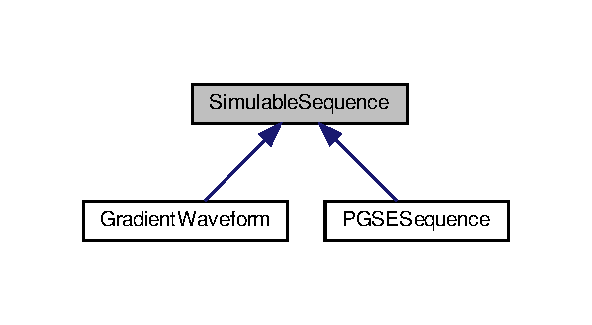
\includegraphics[width=284pt]{class_simulable_sequence__inherit__graph}
\end{center}
\end{figure}
\subsection*{Public Member Functions}
\begin{DoxyCompactItemize}
\item 
virtual void \hyperlink{class_simulable_sequence_a03a417776f5404b06c761ab9109e3e1d}{get\+Grad\+Impulse} (int i, double t, double t\+Last, Eigen\+::\+Vector3d \&Gdt)=0
\item 
virtual double \hyperlink{class_simulable_sequence_a85cdcf5f7bd5bed804a816e3c18840b7}{getb\+Value} (unsigned i)
\item 
\mbox{\Hypertarget{class_simulable_sequence_a31a328cc716e039a53f9b12122050b83}\label{class_simulable_sequence_a31a328cc716e039a53f9b12122050b83}} 
virtual double \hyperlink{class_simulable_sequence_a31a328cc716e039a53f9b12122050b83}{get\+Free\+Decay} (unsigned i, double D)
\begin{DoxyCompactList}\small\item\em Expected free Decay. \end{DoxyCompactList}\item 
virtual void \hyperlink{class_simulable_sequence_ad7b2a30f563343aa65489aa553d4df63}{update\+\_\+phase\+\_\+shift} (double dt, double dt\+\_\+last, \hyperlink{class_walker}{Walker} walker)=0
\item 
virtual void \hyperlink{class_simulable_sequence_a175197d165ee7852094bc70cadc59589}{update\+\_\+phase\+\_\+shift} (double time\+\_\+step, Eigen\+::\+Matrix3\+Xd trajectory)=0
\item 
\mbox{\Hypertarget{class_simulable_sequence_af5621196178ee78b27e740dfe360815e}\label{class_simulable_sequence_af5621196178ee78b27e740dfe360815e}} 
virtual void \hyperlink{class_simulable_sequence_af5621196178ee78b27e740dfe360815e}{update\+\_\+\+D\+W\+I\+\_\+signal} (\hyperlink{class_walker}{Walker} \&walker)=0
\begin{DoxyCompactList}\small\item\em Updates the D\+WI signal using the cumulated phase shift. \end{DoxyCompactList}\item 
\mbox{\Hypertarget{class_simulable_sequence_a2e16c0b0dcf1b90ad0afc53ab14e9250}\label{class_simulable_sequence_a2e16c0b0dcf1b90ad0afc53ab14e9250}} 
virtual void \hyperlink{class_simulable_sequence_a2e16c0b0dcf1b90ad0afc53ab14e9250}{set\+Number\+Of\+Steps} (unsigned T)=0
\begin{DoxyCompactList}\small\item\em Set the number of time steps if they are known. \end{DoxyCompactList}\item 
\mbox{\Hypertarget{class_simulable_sequence_a3c5285531564cdb204894e6c6fc9204e}\label{class_simulable_sequence_a3c5285531564cdb204894e6c6fc9204e}} 
virtual void \hyperlink{class_simulable_sequence_a3c5285531564cdb204894e6c6fc9204e}{compute\+Dynamic\+Time\+Steps} ()
\begin{DoxyCompactList}\small\item\em Compute the time for all the steps when they are not constant. \end{DoxyCompactList}\item 
\mbox{\Hypertarget{class_simulable_sequence_aa2434c3b2ef59d1cd8b822b8e3a2920c}\label{class_simulable_sequence_aa2434c3b2ef59d1cd8b822b8e3a2920c}} 
virtual void \hyperlink{class_simulable_sequence_aa2434c3b2ef59d1cd8b822b8e3a2920c}{initialize\+Subdivision\+Signals} ()
\begin{DoxyCompactList}\small\item\em Initialize the D\+WI signals for each subdivision. \end{DoxyCompactList}\item 
\mbox{\Hypertarget{class_simulable_sequence_a3fad0e115a2ec07a8b1202608eba698e}\label{class_simulable_sequence_a3fad0e115a2ec07a8b1202608eba698e}} 
virtual void \hyperlink{class_simulable_sequence_a3fad0e115a2ec07a8b1202608eba698e}{initialize\+Intra\+Extra\+Signals} ()
\begin{DoxyCompactList}\small\item\em Initialize the D\+WI signals for each compartment (intra extra) \end{DoxyCompactList}\item 
\mbox{\Hypertarget{class_simulable_sequence_a372f6d9f448c537afde10e30b68428aa}\label{class_simulable_sequence_a372f6d9f448c537afde10e30b68428aa}} 
virtual void {\bfseries write\+Resulting\+Data} (std\+::string output\+\_\+base\+\_\+name)
\item 
\mbox{\Hypertarget{class_simulable_sequence_aa6c72a9d84fda0fe15551f84a28d427d}\label{class_simulable_sequence_aa6c72a9d84fda0fe15551f84a28d427d}} 
virtual void {\bfseries write\+Phase\+Shift\+Distribution} (std\+::string output\+\_\+base\+\_\+name)
\item 
\mbox{\Hypertarget{class_simulable_sequence_a49a95a0735a939b65495be51ce0fb1be}\label{class_simulable_sequence_a49a95a0735a939b65495be51ce0fb1be}} 
virtual void {\bfseries clean\+Phase\+Shift} ()
\item 
\mbox{\Hypertarget{class_simulable_sequence_af8396d72ccbb4ad1e8a403e554b8e8e1}\label{class_simulable_sequence_af8396d72ccbb4ad1e8a403e554b8e8e1}} 
virtual void {\bfseries clean\+D\+W\+I\+Signal} ()
\end{DoxyCompactItemize}
\subsection*{Public Attributes}
\begin{DoxyCompactItemize}
\item 
std\+::string \hyperlink{class_simulable_sequence_a9898335af9d8f639f65b73eeac8efb53}{scheme\+\_\+file}
\item 
std\+::vector$<$ double $>$ \hyperlink{class_simulable_sequence_a083961d839ed1433206ccbc481996409}{D\+WI}
\item 
std\+::vector$<$ double $>$ \hyperlink{class_simulable_sequence_ac64fb8110b769e180283365567bd4158}{D\+W\+I\+\_\+intra}
\item 
std\+::vector$<$ double $>$ \hyperlink{class_simulable_sequence_a49a24269e364bcd02000ba575acc85ed}{D\+W\+I\+\_\+extra}
\item 
std\+::vector$<$ double $>$ \hyperlink{class_simulable_sequence_a3708afa1322d72b59d3be20b740d107c}{D\+W\+Ii}
\item 
std\+::vector$<$ double $>$ \hyperlink{class_simulable_sequence_a8691c0451c305869064862e30986c34c}{phase\+\_\+shift}
\item 
int \hyperlink{class_simulable_sequence_aa524c45db6c27dd21acacf97d7951ac2}{num\+\_\+rep}
\item 
bool \hyperlink{class_simulable_sequence_aa29f58ae224d92dd467a0845bd207324}{save\+\_\+phase\+\_\+shift}
\item 
bool \hyperlink{class_simulable_sequence_a1de2d00a939f550af1947ae25acc4b97}{dynamic}
\item 
double \hyperlink{class_simulable_sequence_a43e046af3bf6c498a5ad232058de8a90}{percent\+\_\+steps\+\_\+in}
\item 
std\+::vector$<$ double $>$ \hyperlink{class_simulable_sequence_a7e7e1a0de6045046061ffccaba4fa5ee}{time\+\_\+steps}
\item 
Eigen\+::\+Array\+X\+Xf \hyperlink{class_simulable_sequence_a4e45e2d935a05a7375b04718a49c9af7}{phase\+\_\+shift\+\_\+distribution}
\item 
std\+::vector$<$ std\+::vector$<$ double $>$ $>$ \hyperlink{class_simulable_sequence_a2686ccfa89396eeadd0a0d4f7842623c}{sub\+\_\+\+D\+WI}
\item 
std\+::vector$<$ std\+::vector$<$ double $>$ $>$ \hyperlink{class_simulable_sequence_a20a947108c3bb80ed45dd8851e777511}{sub\+\_\+\+D\+W\+I\+\_\+intra}
\item 
std\+::vector$<$ std\+::vector$<$ double $>$ $>$ \hyperlink{class_simulable_sequence_ad7157eed5b79cf74c45b4185a2465eb6}{sub\+\_\+\+D\+W\+I\+\_\+extra}
\item 
std\+::vector$<$ std\+::vector$<$ double $>$ $>$ \hyperlink{class_simulable_sequence_a1e958cc7d15337fa3ae0e58c8330f212}{sub\+\_\+\+D\+W\+Ii}
\item 
bool \hyperlink{class_simulable_sequence_ae9e6e581ba16bbf81b693c0e4943bbf9}{subdivision\+\_\+flag} = false
\item 
bool \hyperlink{class_simulable_sequence_a3278d9b5b22b0bfbdd0ce4bef0e1cc85}{separate\+\_\+signal} = false
\item 
bool \hyperlink{class_simulable_sequence_a7603177060550acd31ece2c87fcdd2a9}{img\+\_\+signal} = false
\item 
std\+::vector$<$ \hyperlink{class_subdivision}{Subdivision} $>$ \hyperlink{class_simulable_sequence_a77c721d4650578fdc3f44adfa91c030e}{subdivisions}
\end{DoxyCompactItemize}


\subsection{Detailed Description}
MR Sequence Primary Class =============================================================/. 

Elemental base clase. Abstract class to synthesise the M\+RI signal

\subsection*{Jonathan Rafael }

\subsection{Member Function Documentation}
\mbox{\Hypertarget{class_simulable_sequence_a85cdcf5f7bd5bed804a816e3c18840b7}\label{class_simulable_sequence_a85cdcf5f7bd5bed804a816e3c18840b7}} 
\index{Simulable\+Sequence@{Simulable\+Sequence}!getb\+Value@{getb\+Value}}
\index{getb\+Value@{getb\+Value}!Simulable\+Sequence@{Simulable\+Sequence}}
\subsubsection{\texorpdfstring{getb\+Value()}{getbValue()}}
{\footnotesize\ttfamily virtual double Simulable\+Sequence\+::getb\+Value (\begin{DoxyParamCaption}\item[{unsigned}]{i }\end{DoxyParamCaption})\hspace{0.3cm}{\ttfamily [inline]}, {\ttfamily [virtual]}}


\begin{DoxyParams}{Parameters}
{\em i} & index of the gradient in the scheme\+\_\+file (0,N-\/1) \\
\hline
\end{DoxyParams}
\begin{DoxyReturn}{Returns}
b-\/value 
\end{DoxyReturn}


Reimplemented in \hyperlink{class_p_g_s_e_sequence_a8b0671a505f79a601d3d4d2d9b7f36cc}{P\+G\+S\+E\+Sequence}.

\mbox{\Hypertarget{class_simulable_sequence_a03a417776f5404b06c761ab9109e3e1d}\label{class_simulable_sequence_a03a417776f5404b06c761ab9109e3e1d}} 
\index{Simulable\+Sequence@{Simulable\+Sequence}!get\+Grad\+Impulse@{get\+Grad\+Impulse}}
\index{get\+Grad\+Impulse@{get\+Grad\+Impulse}!Simulable\+Sequence@{Simulable\+Sequence}}
\subsubsection{\texorpdfstring{get\+Grad\+Impulse()}{getGradImpulse()}}
{\footnotesize\ttfamily virtual void Simulable\+Sequence\+::get\+Grad\+Impulse (\begin{DoxyParamCaption}\item[{int}]{i,  }\item[{double}]{t,  }\item[{double}]{t\+Last,  }\item[{Eigen\+::\+Vector3d \&}]{Gdt }\end{DoxyParamCaption})\hspace{0.3cm}{\ttfamily [pure virtual]}}


\begin{DoxyParams}{Parameters}
{\em i} & \hyperlink{class_walker}{Walker} index \\
\hline
{\em t} & current time step (in milisenconds) \\
\hline
{\em t\+Last} & last time step (in milisenconds) \\
\hline
{\em Gdt} & vector to compute de G$\ast$dt impulse \\
\hline
\end{DoxyParams}


Implemented in \hyperlink{class_gradient_waveform_a80dd810cb4e5a11dec311ac87e55ea18}{Gradient\+Waveform}, and \hyperlink{class_p_g_s_e_sequence_a3f2a705b7d3312944630f3d7f639e8e4}{P\+G\+S\+E\+Sequence}.

\mbox{\Hypertarget{class_simulable_sequence_ad7b2a30f563343aa65489aa553d4df63}\label{class_simulable_sequence_ad7b2a30f563343aa65489aa553d4df63}} 
\index{Simulable\+Sequence@{Simulable\+Sequence}!update\+\_\+phase\+\_\+shift@{update\+\_\+phase\+\_\+shift}}
\index{update\+\_\+phase\+\_\+shift@{update\+\_\+phase\+\_\+shift}!Simulable\+Sequence@{Simulable\+Sequence}}
\subsubsection{\texorpdfstring{update\+\_\+phase\+\_\+shift()}{update\_phase\_shift()}\hspace{0.1cm}{\footnotesize\ttfamily [1/2]}}
{\footnotesize\ttfamily virtual void Simulable\+Sequence\+::update\+\_\+phase\+\_\+shift (\begin{DoxyParamCaption}\item[{double}]{dt,  }\item[{double}]{dt\+\_\+last,  }\item[{\hyperlink{class_walker}{Walker}}]{walker }\end{DoxyParamCaption})\hspace{0.3cm}{\ttfamily [pure virtual]}}


\begin{DoxyParams}{Parameters}
{\em i} & updated walker \\
\hline
\end{DoxyParams}


Implemented in \hyperlink{class_p_g_s_e_sequence_a6914efd208eab28a1ee6a3f28ca65478}{P\+G\+S\+E\+Sequence}, and \hyperlink{class_gradient_waveform_a7421301b24b6c98e28ef9430287cdf8e}{Gradient\+Waveform}.

\mbox{\Hypertarget{class_simulable_sequence_a175197d165ee7852094bc70cadc59589}\label{class_simulable_sequence_a175197d165ee7852094bc70cadc59589}} 
\index{Simulable\+Sequence@{Simulable\+Sequence}!update\+\_\+phase\+\_\+shift@{update\+\_\+phase\+\_\+shift}}
\index{update\+\_\+phase\+\_\+shift@{update\+\_\+phase\+\_\+shift}!Simulable\+Sequence@{Simulable\+Sequence}}
\subsubsection{\texorpdfstring{update\+\_\+phase\+\_\+shift()}{update\_phase\_shift()}\hspace{0.1cm}{\footnotesize\ttfamily [2/2]}}
{\footnotesize\ttfamily virtual void Simulable\+Sequence\+::update\+\_\+phase\+\_\+shift (\begin{DoxyParamCaption}\item[{double}]{time\+\_\+step,  }\item[{Eigen\+::\+Matrix3\+Xd}]{trajectory }\end{DoxyParamCaption})\hspace{0.3cm}{\ttfamily [pure virtual]}}


\begin{DoxyParams}{Parameters}
{\em i} & updated the phase shift over a whole trajectory \\
\hline
\end{DoxyParams}


Implemented in \hyperlink{class_p_g_s_e_sequence_a850a2f22cdf8b420888cfa906e03e078}{P\+G\+S\+E\+Sequence}, and \hyperlink{class_gradient_waveform_a2c606400c648cebd85827efa8d22b6bc}{Gradient\+Waveform}.



\subsection{Member Data Documentation}
\mbox{\Hypertarget{class_simulable_sequence_a083961d839ed1433206ccbc481996409}\label{class_simulable_sequence_a083961d839ed1433206ccbc481996409}} 
\index{Simulable\+Sequence@{Simulable\+Sequence}!D\+WI@{D\+WI}}
\index{D\+WI@{D\+WI}!Simulable\+Sequence@{Simulable\+Sequence}}
\subsubsection{\texorpdfstring{D\+WI}{DWI}}
{\footnotesize\ttfamily std\+::vector$<$double$>$ Simulable\+Sequence\+::\+D\+WI}

Real part of the D\+WI signal \mbox{\Hypertarget{class_simulable_sequence_a49a24269e364bcd02000ba575acc85ed}\label{class_simulable_sequence_a49a24269e364bcd02000ba575acc85ed}} 
\index{Simulable\+Sequence@{Simulable\+Sequence}!D\+W\+I\+\_\+extra@{D\+W\+I\+\_\+extra}}
\index{D\+W\+I\+\_\+extra@{D\+W\+I\+\_\+extra}!Simulable\+Sequence@{Simulable\+Sequence}}
\subsubsection{\texorpdfstring{D\+W\+I\+\_\+extra}{DWI\_extra}}
{\footnotesize\ttfamily std\+::vector$<$double$>$ Simulable\+Sequence\+::\+D\+W\+I\+\_\+extra}

Real part of the D\+WI signal extra axonal only (if needed) \mbox{\Hypertarget{class_simulable_sequence_ac64fb8110b769e180283365567bd4158}\label{class_simulable_sequence_ac64fb8110b769e180283365567bd4158}} 
\index{Simulable\+Sequence@{Simulable\+Sequence}!D\+W\+I\+\_\+intra@{D\+W\+I\+\_\+intra}}
\index{D\+W\+I\+\_\+intra@{D\+W\+I\+\_\+intra}!Simulable\+Sequence@{Simulable\+Sequence}}
\subsubsection{\texorpdfstring{D\+W\+I\+\_\+intra}{DWI\_intra}}
{\footnotesize\ttfamily std\+::vector$<$double$>$ Simulable\+Sequence\+::\+D\+W\+I\+\_\+intra}

Real part of the D\+WI signal intra axonal olny (if needed) \mbox{\Hypertarget{class_simulable_sequence_a3708afa1322d72b59d3be20b740d107c}\label{class_simulable_sequence_a3708afa1322d72b59d3be20b740d107c}} 
\index{Simulable\+Sequence@{Simulable\+Sequence}!D\+W\+Ii@{D\+W\+Ii}}
\index{D\+W\+Ii@{D\+W\+Ii}!Simulable\+Sequence@{Simulable\+Sequence}}
\subsubsection{\texorpdfstring{D\+W\+Ii}{DWIi}}
{\footnotesize\ttfamily std\+::vector$<$double$>$ Simulable\+Sequence\+::\+D\+W\+Ii}

imaginary part of the D\+WI signal \mbox{\Hypertarget{class_simulable_sequence_a1de2d00a939f550af1947ae25acc4b97}\label{class_simulable_sequence_a1de2d00a939f550af1947ae25acc4b97}} 
\index{Simulable\+Sequence@{Simulable\+Sequence}!dynamic@{dynamic}}
\index{dynamic@{dynamic}!Simulable\+Sequence@{Simulable\+Sequence}}
\subsubsection{\texorpdfstring{dynamic}{dynamic}}
{\footnotesize\ttfamily bool Simulable\+Sequence\+::dynamic}

Flag to indicate if the time steps are non-\/uniform \mbox{\Hypertarget{class_simulable_sequence_a7603177060550acd31ece2c87fcdd2a9}\label{class_simulable_sequence_a7603177060550acd31ece2c87fcdd2a9}} 
\index{Simulable\+Sequence@{Simulable\+Sequence}!img\+\_\+signal@{img\+\_\+signal}}
\index{img\+\_\+signal@{img\+\_\+signal}!Simulable\+Sequence@{Simulable\+Sequence}}
\subsubsection{\texorpdfstring{img\+\_\+signal}{img\_signal}}
{\footnotesize\ttfamily bool Simulable\+Sequence\+::img\+\_\+signal = false}

flag to check if the img part will be computed or not (false default \mbox{\Hypertarget{class_simulable_sequence_aa524c45db6c27dd21acacf97d7951ac2}\label{class_simulable_sequence_aa524c45db6c27dd21acacf97d7951ac2}} 
\index{Simulable\+Sequence@{Simulable\+Sequence}!num\+\_\+rep@{num\+\_\+rep}}
\index{num\+\_\+rep@{num\+\_\+rep}!Simulable\+Sequence@{Simulable\+Sequence}}
\subsubsection{\texorpdfstring{num\+\_\+rep}{num\_rep}}
{\footnotesize\ttfamily int Simulable\+Sequence\+::num\+\_\+rep}

number of repetitions . \mbox{\Hypertarget{class_simulable_sequence_a43e046af3bf6c498a5ad232058de8a90}\label{class_simulable_sequence_a43e046af3bf6c498a5ad232058de8a90}} 
\index{Simulable\+Sequence@{Simulable\+Sequence}!percent\+\_\+steps\+\_\+in@{percent\+\_\+steps\+\_\+in}}
\index{percent\+\_\+steps\+\_\+in@{percent\+\_\+steps\+\_\+in}!Simulable\+Sequence@{Simulable\+Sequence}}
\subsubsection{\texorpdfstring{percent\+\_\+steps\+\_\+in}{percent\_steps\_in}}
{\footnotesize\ttfamily double Simulable\+Sequence\+::percent\+\_\+steps\+\_\+in}

percentage of steps that should be inside the gradient times \mbox{\Hypertarget{class_simulable_sequence_a8691c0451c305869064862e30986c34c}\label{class_simulable_sequence_a8691c0451c305869064862e30986c34c}} 
\index{Simulable\+Sequence@{Simulable\+Sequence}!phase\+\_\+shift@{phase\+\_\+shift}}
\index{phase\+\_\+shift@{phase\+\_\+shift}!Simulable\+Sequence@{Simulable\+Sequence}}
\subsubsection{\texorpdfstring{phase\+\_\+shift}{phase\_shift}}
{\footnotesize\ttfamily std\+::vector$<$double$>$ Simulable\+Sequence\+::phase\+\_\+shift}

auxiliar phase shift for signal computations. \mbox{\Hypertarget{class_simulable_sequence_a4e45e2d935a05a7375b04718a49c9af7}\label{class_simulable_sequence_a4e45e2d935a05a7375b04718a49c9af7}} 
\index{Simulable\+Sequence@{Simulable\+Sequence}!phase\+\_\+shift\+\_\+distribution@{phase\+\_\+shift\+\_\+distribution}}
\index{phase\+\_\+shift\+\_\+distribution@{phase\+\_\+shift\+\_\+distribution}!Simulable\+Sequence@{Simulable\+Sequence}}
\subsubsection{\texorpdfstring{phase\+\_\+shift\+\_\+distribution}{phase\_shift\_distribution}}
{\footnotesize\ttfamily Eigen\+::\+Array\+X\+Xf Simulable\+Sequence\+::phase\+\_\+shift\+\_\+distribution}

Matrix to save the phase shif distribution \mbox{\Hypertarget{class_simulable_sequence_aa29f58ae224d92dd467a0845bd207324}\label{class_simulable_sequence_aa29f58ae224d92dd467a0845bd207324}} 
\index{Simulable\+Sequence@{Simulable\+Sequence}!save\+\_\+phase\+\_\+shift@{save\+\_\+phase\+\_\+shift}}
\index{save\+\_\+phase\+\_\+shift@{save\+\_\+phase\+\_\+shift}!Simulable\+Sequence@{Simulable\+Sequence}}
\subsubsection{\texorpdfstring{save\+\_\+phase\+\_\+shift}{save\_phase\_shift}}
{\footnotesize\ttfamily bool Simulable\+Sequence\+::save\+\_\+phase\+\_\+shift}

flag, if true, saves the pahse shift distribution. \mbox{\Hypertarget{class_simulable_sequence_a9898335af9d8f639f65b73eeac8efb53}\label{class_simulable_sequence_a9898335af9d8f639f65b73eeac8efb53}} 
\index{Simulable\+Sequence@{Simulable\+Sequence}!scheme\+\_\+file@{scheme\+\_\+file}}
\index{scheme\+\_\+file@{scheme\+\_\+file}!Simulable\+Sequence@{Simulable\+Sequence}}
\subsubsection{\texorpdfstring{scheme\+\_\+file}{scheme\_file}}
{\footnotesize\ttfamily std\+::string Simulable\+Sequence\+::scheme\+\_\+file}

\hyperlink{class_scheme}{Scheme} file path \mbox{\Hypertarget{class_simulable_sequence_a3278d9b5b22b0bfbdd0ce4bef0e1cc85}\label{class_simulable_sequence_a3278d9b5b22b0bfbdd0ce4bef0e1cc85}} 
\index{Simulable\+Sequence@{Simulable\+Sequence}!separate\+\_\+signal@{separate\+\_\+signal}}
\index{separate\+\_\+signal@{separate\+\_\+signal}!Simulable\+Sequence@{Simulable\+Sequence}}
\subsubsection{\texorpdfstring{separate\+\_\+signal}{separate\_signal}}
{\footnotesize\ttfamily bool Simulable\+Sequence\+::separate\+\_\+signal = false}

flag to check if we will separate the signal in intra and extra \mbox{\Hypertarget{class_simulable_sequence_a2686ccfa89396eeadd0a0d4f7842623c}\label{class_simulable_sequence_a2686ccfa89396eeadd0a0d4f7842623c}} 
\index{Simulable\+Sequence@{Simulable\+Sequence}!sub\+\_\+\+D\+WI@{sub\+\_\+\+D\+WI}}
\index{sub\+\_\+\+D\+WI@{sub\+\_\+\+D\+WI}!Simulable\+Sequence@{Simulable\+Sequence}}
\subsubsection{\texorpdfstring{sub\+\_\+\+D\+WI}{sub\_DWI}}
{\footnotesize\ttfamily std\+::vector$<$std\+::vector$<$double$>$ $>$ Simulable\+Sequence\+::sub\+\_\+\+D\+WI}

Real part of the D\+WI signal for each sub\+Division \mbox{\Hypertarget{class_simulable_sequence_ad7157eed5b79cf74c45b4185a2465eb6}\label{class_simulable_sequence_ad7157eed5b79cf74c45b4185a2465eb6}} 
\index{Simulable\+Sequence@{Simulable\+Sequence}!sub\+\_\+\+D\+W\+I\+\_\+extra@{sub\+\_\+\+D\+W\+I\+\_\+extra}}
\index{sub\+\_\+\+D\+W\+I\+\_\+extra@{sub\+\_\+\+D\+W\+I\+\_\+extra}!Simulable\+Sequence@{Simulable\+Sequence}}
\subsubsection{\texorpdfstring{sub\+\_\+\+D\+W\+I\+\_\+extra}{sub\_DWI\_extra}}
{\footnotesize\ttfamily std\+::vector$<$std\+::vector$<$double$>$ $>$ Simulable\+Sequence\+::sub\+\_\+\+D\+W\+I\+\_\+extra}

Real part of the D\+WI extra signal for each sub\+Division \mbox{\Hypertarget{class_simulable_sequence_a20a947108c3bb80ed45dd8851e777511}\label{class_simulable_sequence_a20a947108c3bb80ed45dd8851e777511}} 
\index{Simulable\+Sequence@{Simulable\+Sequence}!sub\+\_\+\+D\+W\+I\+\_\+intra@{sub\+\_\+\+D\+W\+I\+\_\+intra}}
\index{sub\+\_\+\+D\+W\+I\+\_\+intra@{sub\+\_\+\+D\+W\+I\+\_\+intra}!Simulable\+Sequence@{Simulable\+Sequence}}
\subsubsection{\texorpdfstring{sub\+\_\+\+D\+W\+I\+\_\+intra}{sub\_DWI\_intra}}
{\footnotesize\ttfamily std\+::vector$<$std\+::vector$<$double$>$ $>$ Simulable\+Sequence\+::sub\+\_\+\+D\+W\+I\+\_\+intra}

Real part of the D\+WI intra signal for each sub\+Division \mbox{\Hypertarget{class_simulable_sequence_a1e958cc7d15337fa3ae0e58c8330f212}\label{class_simulable_sequence_a1e958cc7d15337fa3ae0e58c8330f212}} 
\index{Simulable\+Sequence@{Simulable\+Sequence}!sub\+\_\+\+D\+W\+Ii@{sub\+\_\+\+D\+W\+Ii}}
\index{sub\+\_\+\+D\+W\+Ii@{sub\+\_\+\+D\+W\+Ii}!Simulable\+Sequence@{Simulable\+Sequence}}
\subsubsection{\texorpdfstring{sub\+\_\+\+D\+W\+Ii}{sub\_DWIi}}
{\footnotesize\ttfamily std\+::vector$<$std\+::vector$<$double$>$ $>$ Simulable\+Sequence\+::sub\+\_\+\+D\+W\+Ii}

Imaginary part of the D\+WI signal for each subdivision \mbox{\Hypertarget{class_simulable_sequence_ae9e6e581ba16bbf81b693c0e4943bbf9}\label{class_simulable_sequence_ae9e6e581ba16bbf81b693c0e4943bbf9}} 
\index{Simulable\+Sequence@{Simulable\+Sequence}!subdivision\+\_\+flag@{subdivision\+\_\+flag}}
\index{subdivision\+\_\+flag@{subdivision\+\_\+flag}!Simulable\+Sequence@{Simulable\+Sequence}}
\subsubsection{\texorpdfstring{subdivision\+\_\+flag}{subdivision\_flag}}
{\footnotesize\ttfamily bool Simulable\+Sequence\+::subdivision\+\_\+flag = false}

flag to check if we have several voxel subdivision to compute the signal \mbox{\Hypertarget{class_simulable_sequence_a77c721d4650578fdc3f44adfa91c030e}\label{class_simulable_sequence_a77c721d4650578fdc3f44adfa91c030e}} 
\index{Simulable\+Sequence@{Simulable\+Sequence}!subdivisions@{subdivisions}}
\index{subdivisions@{subdivisions}!Simulable\+Sequence@{Simulable\+Sequence}}
\subsubsection{\texorpdfstring{subdivisions}{subdivisions}}
{\footnotesize\ttfamily std\+::vector$<$\hyperlink{class_subdivision}{Subdivision}$>$ Simulable\+Sequence\+::subdivisions}

saves the actual positions of the subdivision to compute the signal \mbox{\Hypertarget{class_simulable_sequence_a7e7e1a0de6045046061ffccaba4fa5ee}\label{class_simulable_sequence_a7e7e1a0de6045046061ffccaba4fa5ee}} 
\index{Simulable\+Sequence@{Simulable\+Sequence}!time\+\_\+steps@{time\+\_\+steps}}
\index{time\+\_\+steps@{time\+\_\+steps}!Simulable\+Sequence@{Simulable\+Sequence}}
\subsubsection{\texorpdfstring{time\+\_\+steps}{time\_steps}}
{\footnotesize\ttfamily std\+::vector$<$double$>$ Simulable\+Sequence\+::time\+\_\+steps}

Auxiliary array to save the time steps 

The documentation for this class was generated from the following files\+:\begin{DoxyCompactItemize}
\item 
src/simulablesequence.\+h\item 
src/simulablesequence.\+cpp\end{DoxyCompactItemize}

\hypertarget{class_subdivision}{}\section{Subdivision Class Reference}
\label{class_subdivision}\index{Subdivision@{Subdivision}}


Auxiliary \hyperlink{class_subdivision}{Subdivision} Class =============================================================/.  




{\ttfamily \#include $<$subdivision.\+h$>$}

\subsection*{Public Member Functions}
\begin{DoxyCompactItemize}
\item 
\mbox{\Hypertarget{class_subdivision_ac51db3c00b0e4f7543c34859ad846871}\label{class_subdivision_ac51db3c00b0e4f7543c34859ad846871}} 
\hyperlink{class_subdivision_ac51db3c00b0e4f7543c34859ad846871}{Subdivision} ()
\begin{DoxyCompactList}\small\item\em Naive constructor. \end{DoxyCompactList}\item 
\mbox{\Hypertarget{class_subdivision_a96a55a5e9c88a2ee0640a904bb30141c}\label{class_subdivision_a96a55a5e9c88a2ee0640a904bb30141c}} 
\hyperlink{class_subdivision_a96a55a5e9c88a2ee0640a904bb30141c}{Subdivision} (Eigen\+::\+Vector3f \&, Eigen\+::\+Vector3f \&)
\begin{DoxyCompactList}\small\item\em Constructor for a defined list of min and max positions. \end{DoxyCompactList}\item 
bool \hyperlink{class_subdivision_adb91e1cc1e6959d13220454ddfc7ba28}{is\+Inside} (Eigen\+::\+Vector3d \&pos)
\begin{DoxyCompactList}\small\item\em Auxiliary function to check if a 3d position is inside a \char`\"{}subdivision\char`\"{} i.\+e. defined cube. \end{DoxyCompactList}\end{DoxyCompactItemize}
\subsection*{Public Attributes}
\begin{DoxyCompactItemize}
\item 
Eigen\+::\+Vector3f \hyperlink{class_subdivision_ac8d84e208bb294b78379a05da4ccfc37}{min\+\_\+limits}
\item 
Eigen\+::\+Vector3f \hyperlink{class_subdivision_a96ca3e7e744026fef809ade08d861985}{max\+\_\+limits}
\item 
int \hyperlink{class_subdivision_a6135c9e9b9a16f2f316d28071dee16c6}{density}
\item 
int \hyperlink{class_subdivision_a2944862a3bafcacaf45a935f266f0cf0}{density\+\_\+intra}
\item 
int \hyperlink{class_subdivision_aa9d564a68a0785998db3e129c6698c0f}{density\+\_\+extra}
\end{DoxyCompactItemize}


\subsection{Detailed Description}
Auxiliary \hyperlink{class_subdivision}{Subdivision} Class =============================================================/. 

Auxiliary Class. Implementation of the subdivision of a voxel into separate adquisitions

\begin{DoxyDate}{Date}
September 2017 
\end{DoxyDate}
\begin{DoxyAuthor}{Author}
Jonathan Rafael \subsection*{0.\+1.\+0 }
\end{DoxyAuthor}


\subsection{Member Function Documentation}
\mbox{\Hypertarget{class_subdivision_adb91e1cc1e6959d13220454ddfc7ba28}\label{class_subdivision_adb91e1cc1e6959d13220454ddfc7ba28}} 
\index{Subdivision@{Subdivision}!is\+Inside@{is\+Inside}}
\index{is\+Inside@{is\+Inside}!Subdivision@{Subdivision}}
\subsubsection{\texorpdfstring{is\+Inside()}{isInside()}}
{\footnotesize\ttfamily bool Subdivision\+::is\+Inside (\begin{DoxyParamCaption}\item[{Eigen\+::\+Vector3d \&}]{pos }\end{DoxyParamCaption})}



Auxiliary function to check if a 3d position is inside a \char`\"{}subdivision\char`\"{} i.\+e. defined cube. 


\begin{DoxyParams}{Parameters}
{\em pos} & 3d position \\
\hline
\end{DoxyParams}


\subsection{Member Data Documentation}
\mbox{\Hypertarget{class_subdivision_a6135c9e9b9a16f2f316d28071dee16c6}\label{class_subdivision_a6135c9e9b9a16f2f316d28071dee16c6}} 
\index{Subdivision@{Subdivision}!density@{density}}
\index{density@{density}!Subdivision@{Subdivision}}
\subsubsection{\texorpdfstring{density}{density}}
{\footnotesize\ttfamily int Subdivision\+::density}

Counter to save the number of particles inside that region \mbox{\Hypertarget{class_subdivision_aa9d564a68a0785998db3e129c6698c0f}\label{class_subdivision_aa9d564a68a0785998db3e129c6698c0f}} 
\index{Subdivision@{Subdivision}!density\+\_\+extra@{density\+\_\+extra}}
\index{density\+\_\+extra@{density\+\_\+extra}!Subdivision@{Subdivision}}
\subsubsection{\texorpdfstring{density\+\_\+extra}{density\_extra}}
{\footnotesize\ttfamily int Subdivision\+::density\+\_\+extra}

Counter to save the number of particles labeled as Extra in that region \mbox{\Hypertarget{class_subdivision_a2944862a3bafcacaf45a935f266f0cf0}\label{class_subdivision_a2944862a3bafcacaf45a935f266f0cf0}} 
\index{Subdivision@{Subdivision}!density\+\_\+intra@{density\+\_\+intra}}
\index{density\+\_\+intra@{density\+\_\+intra}!Subdivision@{Subdivision}}
\subsubsection{\texorpdfstring{density\+\_\+intra}{density\_intra}}
{\footnotesize\ttfamily int Subdivision\+::density\+\_\+intra}

Counter to save the number of particles labeled as Intra in that region \mbox{\Hypertarget{class_subdivision_a96ca3e7e744026fef809ade08d861985}\label{class_subdivision_a96ca3e7e744026fef809ade08d861985}} 
\index{Subdivision@{Subdivision}!max\+\_\+limits@{max\+\_\+limits}}
\index{max\+\_\+limits@{max\+\_\+limits}!Subdivision@{Subdivision}}
\subsubsection{\texorpdfstring{max\+\_\+limits}{max\_limits}}
{\footnotesize\ttfamily Eigen\+::\+Vector3f Subdivision\+::max\+\_\+limits}

Vector with the list of max limits points of each subdivisions \mbox{\Hypertarget{class_subdivision_ac8d84e208bb294b78379a05da4ccfc37}\label{class_subdivision_ac8d84e208bb294b78379a05da4ccfc37}} 
\index{Subdivision@{Subdivision}!min\+\_\+limits@{min\+\_\+limits}}
\index{min\+\_\+limits@{min\+\_\+limits}!Subdivision@{Subdivision}}
\subsubsection{\texorpdfstring{min\+\_\+limits}{min\_limits}}
{\footnotesize\ttfamily Eigen\+::\+Vector3f Subdivision\+::min\+\_\+limits}

Vector with the list of min limits points of each subdivisions 

The documentation for this class was generated from the following files\+:\begin{DoxyCompactItemize}
\item 
src/subdivision.\+h\item 
src/subdivision.\+cpp\end{DoxyCompactItemize}

\hypertarget{class_trajectory}{}\section{Trajectory Class Reference}
\label{class_trajectory}\index{Trajectory@{Trajectory}}


Auxiliary class. Handles i/o operation of walker trayectories. ============================/.  




{\ttfamily \#include $<$trajectory.\+h$>$}

\subsection*{Public Member Functions}
\begin{DoxyCompactItemize}
\item 
\mbox{\Hypertarget{class_trajectory_aa340ba80f1f4d1aa39f19f069d5d8089}\label{class_trajectory_aa340ba80f1f4d1aa39f19f069d5d8089}} 
\hyperlink{class_trajectory_aa340ba80f1f4d1aa39f19f069d5d8089}{Trajectory} ()
\begin{DoxyCompactList}\small\item\em Main constructor, Initialice everythin to default. \end{DoxyCompactList}\item 
\mbox{\Hypertarget{class_trajectory_a4879a4d0944eb04246e21deac940b90d}\label{class_trajectory_a4879a4d0944eb04246e21deac940b90d}} 
\hyperlink{class_trajectory_a4879a4d0944eb04246e21deac940b90d}{Trajectory} (const char $\ast$traj\+\_\+file, bool is\+Big\+Endian\+\_\+=true, std\+::string io\+\_\+flag\+\_\+=\char`\"{}rb\char`\"{})
\begin{DoxyCompactList}\small\item\em Contructor , Initialice everythin by parameters. \end{DoxyCompactList}\item 
\mbox{\Hypertarget{class_trajectory_ac673c37025ca5353ad99ab41c936e75d}\label{class_trajectory_ac673c37025ca5353ad99ab41c936e75d}} 
\hyperlink{class_trajectory_ac673c37025ca5353ad99ab41c936e75d}{$\sim$\+Trajectory} ()
\begin{DoxyCompactList}\small\item\em Destructor, close files and fstreams. \end{DoxyCompactList}\item 
\mbox{\Hypertarget{class_trajectory_aaeda8b05ad61298fbd2aba2a3192486e}\label{class_trajectory_aaeda8b05ad61298fbd2aba2a3192486e}} 
void \hyperlink{class_trajectory_aaeda8b05ad61298fbd2aba2a3192486e}{init\+Trajectory} (\hyperlink{class_parameters}{Parameters} params)
\begin{DoxyCompactList}\small\item\em Initialice the output files if any. \end{DoxyCompactList}\item 
\mbox{\Hypertarget{class_trajectory_a00a28c1782a0a661b40ad9dfefc0d3f4}\label{class_trajectory_a00a28c1782a0a661b40ad9dfefc0d3f4}} 
void \hyperlink{class_trajectory_a00a28c1782a0a661b40ad9dfefc0d3f4}{set\+Traj\+File} (std\+::string)
\begin{DoxyCompactList}\small\item\em Setd the traj file operations. \end{DoxyCompactList}\end{DoxyCompactItemize}
\textbf{ }\par
\begin{DoxyCompactItemize}
\item 
void \hyperlink{class_trajectory_a9aedf2530dca72ca629741585717c64a}{close\+Traj\+Reader\+File} ()
\item 
\mbox{\Hypertarget{class_trajectory_a9239f7d5d05f02ce58b6ad2e7be231d7}\label{class_trajectory_a9239f7d5d05f02ce58b6ad2e7be231d7}} 
void {\bfseries open\+Traj\+Reader\+File} ()
\item 
\mbox{\Hypertarget{class_trajectory_a727883a1c29c9bdb8d4cdb01888023da}\label{class_trajectory_a727883a1c29c9bdb8d4cdb01888023da}} 
void {\bfseries init\+Traj\+Reader\+File} ()
\item 
\mbox{\Hypertarget{class_trajectory_ad436905c5614d4ac3a52acb6d2211b61}\label{class_trajectory_ad436905c5614d4ac3a52acb6d2211b61}} 
void {\bfseries read\+Trajectory\+Header} ()
\item 
\mbox{\Hypertarget{class_trajectory_a5f96383db2d95b41a46dc752b00f70e6}\label{class_trajectory_a5f96383db2d95b41a46dc752b00f70e6}} 
void {\bfseries read\+Current\+Walkers\+Trajectory} (Eigen\+::\+Matrix3\+Xd \&)
\end{DoxyCompactItemize}

\textbf{ }\par
\begin{DoxyCompactItemize}
\item 
void \hyperlink{class_trajectory_aec9f75fa04452af2199888c47652c7e4}{init\+Traj\+Writer} ()
\item 
\mbox{\Hypertarget{class_trajectory_a661b8c4070a55fd2e6abe703d23c95df}\label{class_trajectory_a661b8c4070a55fd2e6abe703d23c95df}} 
void {\bfseries init\+Traj\+Writer\+Binary} ()
\item 
\mbox{\Hypertarget{class_trajectory_a7b6926793185fc0ebebb09a7abba8b7a}\label{class_trajectory_a7b6926793185fc0ebebb09a7abba8b7a}} 
void {\bfseries init\+Traj\+Writer\+Text} ()
\item 
\mbox{\Hypertarget{class_trajectory_a0cf9e0365b4d075d2da7c800fef83858}\label{class_trajectory_a0cf9e0365b4d075d2da7c800fef83858}} 
void {\bfseries write\+Trajectory\+Header\+Binary} ()
\item 
\mbox{\Hypertarget{class_trajectory_ae84e1c1573c8f42bd68c09dff3909f6f}\label{class_trajectory_ae84e1c1573c8f42bd68c09dff3909f6f}} 
void {\bfseries write\+Trajectory\+Header\+Text} ()
\item 
\mbox{\Hypertarget{class_trajectory_a82540862cb8c200b1a6979b5f919681d}\label{class_trajectory_a82540862cb8c200b1a6979b5f919681d}} 
void {\bfseries re\+Write\+Header\+File} (unsigned num\+\_\+walkers)
\item 
\mbox{\Hypertarget{class_trajectory_ada4c4918a46c69508e6e847e4ef54f56}\label{class_trajectory_ada4c4918a46c69508e6e847e4ef54f56}} 
void {\bfseries write\+Position} (Eigen\+::\+Vector3d \&)
\item 
\mbox{\Hypertarget{class_trajectory_ad35ef554146d54b4ea0a3bdce1f6246d}\label{class_trajectory_ad35ef554146d54b4ea0a3bdce1f6246d}} 
void {\bfseries write\+Position\+Text} (Eigen\+::\+Vector3d \&)
\item 
\mbox{\Hypertarget{class_trajectory_a8ab6682b6a6c9cdc78fb6cef56129c91}\label{class_trajectory_a8ab6682b6a6c9cdc78fb6cef56129c91}} 
void {\bfseries write\+Position\+Binary} (Eigen\+::\+Vector3d \&)
\item 
\mbox{\Hypertarget{class_trajectory_a5392bbab8cb315fcb99d30c90ca746b1}\label{class_trajectory_a5392bbab8cb315fcb99d30c90ca746b1}} 
void {\bfseries write\+Position} (Eigen\+::\+Matrix3\+Xd \&)
\item 
\mbox{\Hypertarget{class_trajectory_a85776d999a5eacdbbef9008f96da007b}\label{class_trajectory_a85776d999a5eacdbbef9008f96da007b}} 
void {\bfseries write\+Position\+Text} (Eigen\+::\+Matrix3\+Xd \&)
\item 
\mbox{\Hypertarget{class_trajectory_a0c8e6a22d330cfdb6419813ffd43ccba}\label{class_trajectory_a0c8e6a22d330cfdb6419813ffd43ccba}} 
void {\bfseries write\+Position\+Binary} (Eigen\+::\+Matrix3\+Xd \&)
\end{DoxyCompactItemize}

\subsection*{Public Attributes}
\begin{DoxyCompactItemize}
\item 
std\+::string \hyperlink{class_trajectory_aee056cca538c4430eacff9534e43bc8e}{trajfile}
\item 
std\+::string \hyperlink{class_trajectory_a6bb5d5e4ad4fb36a65d6cffdc6ab05af}{headerfile}
\item 
\mbox{\Hypertarget{class_trajectory_aa6725e54b483f0eaaae88710707e58fe}\label{class_trajectory_aa6725e54b483f0eaaae88710707e58fe}} 
F\+I\+LE $\ast$ {\bfseries in}
\item 
F\+I\+LE $\ast$ \hyperlink{class_trajectory_a6a7484c5282331583841b038997d597b}{in\+\_\+header}
\item 
\mbox{\Hypertarget{class_trajectory_a41053c7c21f625933b4dd290da958b7c}\label{class_trajectory_a41053c7c21f625933b4dd290da958b7c}} 
std\+::ofstream {\bfseries bout}
\item 
\mbox{\Hypertarget{class_trajectory_a2373f0055623b904e6051c0681d13472}\label{class_trajectory_a2373f0055623b904e6051c0681d13472}} 
std\+::ofstream {\bfseries tout}
\item 
\mbox{\Hypertarget{class_trajectory_abf8e0a2b50a2e873c261720e295687ac}\label{class_trajectory_abf8e0a2b50a2e873c261720e295687ac}} 
std\+::ofstream {\bfseries bheaderout}
\item 
\mbox{\Hypertarget{class_trajectory_a90e41427f7c6ce7b5b549e072fd9f59d}\label{class_trajectory_a90e41427f7c6ce7b5b549e072fd9f59d}} 
std\+::ofstream {\bfseries theaderout}
\item 
\mbox{\Hypertarget{class_trajectory_a849e3a9c92a6eea27073c4e533412a67}\label{class_trajectory_a849e3a9c92a6eea27073c4e533412a67}} 
unsigned {\bfseries N}
\item 
unsigned \hyperlink{class_trajectory_ad9cbff5cf9f84ca1e2378d1d6105c5e3}{T}
\item 
\mbox{\Hypertarget{class_trajectory_ada15a7d6836e4cee2f35f788df0d844f}\label{class_trajectory_ada15a7d6836e4cee2f35f788df0d844f}} 
double {\bfseries dyn\+\_\+duration}
\item 
\mbox{\Hypertarget{class_trajectory_abc9b9bb15f5723a208f0ff22cd740eda}\label{class_trajectory_abc9b9bb15f5723a208f0ff22cd740eda}} 
std\+::string {\bfseries io\+\_\+flag}
\item 
std\+::vector$<$ unsigned $>$ \hyperlink{class_trajectory_a4b6369fb83108e27a774f50c06169817}{pos\+\_\+times}
\item 
bool \hyperlink{class_trajectory_a66dfa9e8d1e60706b8e8bb1e91a34e29}{is\+Big\+Endian}
\item 
bool \hyperlink{class_trajectory_a1194477068ed051401f99aba4a1056b1}{write\+\_\+traj}
\item 
bool \hyperlink{class_trajectory_a94125474ee64fd3007091a3e88f59769}{write\+\_\+txt}
\item 
bool \hyperlink{class_trajectory_a7135e87575f429a7d6ad32477dc96e2c}{write\+\_\+bin}
\item 
bool \hyperlink{class_trajectory_a973422e0d41afe4720fbbf62500a5035}{steps\+\_\+subset}
\end{DoxyCompactItemize}


\subsection{Detailed Description}
Auxiliary class. Handles i/o operation of walker trayectories. ============================/. 

\begin{DoxyAuthor}{Author}
Jonathan Rafael 
\end{DoxyAuthor}
\begin{DoxyDate}{Date}
July 2016 \subsection*{0.\+2 }
\end{DoxyDate}


\subsection{Member Function Documentation}
\mbox{\Hypertarget{class_trajectory_a9aedf2530dca72ca629741585717c64a}\label{class_trajectory_a9aedf2530dca72ca629741585717c64a}} 
\index{Trajectory@{Trajectory}!close\+Traj\+Reader\+File@{close\+Traj\+Reader\+File}}
\index{close\+Traj\+Reader\+File@{close\+Traj\+Reader\+File}!Trajectory@{Trajectory}}
\subsubsection{\texorpdfstring{close\+Traj\+Reader\+File()}{closeTrajReaderFile()}}
{\footnotesize\ttfamily void Trajectory\+::close\+Traj\+Reader\+File (\begin{DoxyParamCaption}{ }\end{DoxyParamCaption})}

Read operations \mbox{\Hypertarget{class_trajectory_aec9f75fa04452af2199888c47652c7e4}\label{class_trajectory_aec9f75fa04452af2199888c47652c7e4}} 
\index{Trajectory@{Trajectory}!init\+Traj\+Writer@{init\+Traj\+Writer}}
\index{init\+Traj\+Writer@{init\+Traj\+Writer}!Trajectory@{Trajectory}}
\subsubsection{\texorpdfstring{init\+Traj\+Writer()}{initTrajWriter()}}
{\footnotesize\ttfamily void Trajectory\+::init\+Traj\+Writer (\begin{DoxyParamCaption}{ }\end{DoxyParamCaption})}

Write operations 

\subsection{Member Data Documentation}
\mbox{\Hypertarget{class_trajectory_a6bb5d5e4ad4fb36a65d6cffdc6ab05af}\label{class_trajectory_a6bb5d5e4ad4fb36a65d6cffdc6ab05af}} 
\index{Trajectory@{Trajectory}!headerfile@{headerfile}}
\index{headerfile@{headerfile}!Trajectory@{Trajectory}}
\subsubsection{\texorpdfstring{headerfile}{headerfile}}
{\footnotesize\ttfamily std\+::string Trajectory\+::headerfile}

header name \mbox{\Hypertarget{class_trajectory_a6a7484c5282331583841b038997d597b}\label{class_trajectory_a6a7484c5282331583841b038997d597b}} 
\index{Trajectory@{Trajectory}!in\+\_\+header@{in\+\_\+header}}
\index{in\+\_\+header@{in\+\_\+header}!Trajectory@{Trajectory}}
\subsubsection{\texorpdfstring{in\+\_\+header}{in\_header}}
{\footnotesize\ttfamily F\+I\+LE $\ast$ Trajectory\+::in\+\_\+header}

Files to be written using the previous names binary out, text out, binary header, text header \mbox{\Hypertarget{class_trajectory_a66dfa9e8d1e60706b8e8bb1e91a34e29}\label{class_trajectory_a66dfa9e8d1e60706b8e8bb1e91a34e29}} 
\index{Trajectory@{Trajectory}!is\+Big\+Endian@{is\+Big\+Endian}}
\index{is\+Big\+Endian@{is\+Big\+Endian}!Trajectory@{Trajectory}}
\subsubsection{\texorpdfstring{is\+Big\+Endian}{isBigEndian}}
{\footnotesize\ttfamily bool Trajectory\+::is\+Big\+Endian}

flag if the format is big endian \mbox{\Hypertarget{class_trajectory_a4b6369fb83108e27a774f50c06169817}\label{class_trajectory_a4b6369fb83108e27a774f50c06169817}} 
\index{Trajectory@{Trajectory}!pos\+\_\+times@{pos\+\_\+times}}
\index{pos\+\_\+times@{pos\+\_\+times}!Trajectory@{Trajectory}}
\subsubsection{\texorpdfstring{pos\+\_\+times}{pos\_times}}
{\footnotesize\ttfamily std\+::vector$<$unsigned$>$ Trajectory\+::pos\+\_\+times}

Times indexes when to save the particle positions. \mbox{\Hypertarget{class_trajectory_a973422e0d41afe4720fbbf62500a5035}\label{class_trajectory_a973422e0d41afe4720fbbf62500a5035}} 
\index{Trajectory@{Trajectory}!steps\+\_\+subset@{steps\+\_\+subset}}
\index{steps\+\_\+subset@{steps\+\_\+subset}!Trajectory@{Trajectory}}
\subsubsection{\texorpdfstring{steps\+\_\+subset}{steps\_subset}}
{\footnotesize\ttfamily bool Trajectory\+::steps\+\_\+subset}

true if the steps are no uniform \mbox{\Hypertarget{class_trajectory_ad9cbff5cf9f84ca1e2378d1d6105c5e3}\label{class_trajectory_ad9cbff5cf9f84ca1e2378d1d6105c5e3}} 
\index{Trajectory@{Trajectory}!T@{T}}
\index{T@{T}!Trajectory@{Trajectory}}
\subsubsection{\texorpdfstring{T}{T}}
{\footnotesize\ttfamily unsigned Trajectory\+::T}

number of walkers, total time; \mbox{\Hypertarget{class_trajectory_aee056cca538c4430eacff9534e43bc8e}\label{class_trajectory_aee056cca538c4430eacff9534e43bc8e}} 
\index{Trajectory@{Trajectory}!trajfile@{trajfile}}
\index{trajfile@{trajfile}!Trajectory@{Trajectory}}
\subsubsection{\texorpdfstring{trajfile}{trajfile}}
{\footnotesize\ttfamily std\+::string Trajectory\+::trajfile}

trajfile name \mbox{\Hypertarget{class_trajectory_a7135e87575f429a7d6ad32477dc96e2c}\label{class_trajectory_a7135e87575f429a7d6ad32477dc96e2c}} 
\index{Trajectory@{Trajectory}!write\+\_\+bin@{write\+\_\+bin}}
\index{write\+\_\+bin@{write\+\_\+bin}!Trajectory@{Trajectory}}
\subsubsection{\texorpdfstring{write\+\_\+bin}{write\_bin}}
{\footnotesize\ttfamily bool Trajectory\+::write\+\_\+bin}

flag if we want to write a binary traj file \mbox{\Hypertarget{class_trajectory_a1194477068ed051401f99aba4a1056b1}\label{class_trajectory_a1194477068ed051401f99aba4a1056b1}} 
\index{Trajectory@{Trajectory}!write\+\_\+traj@{write\+\_\+traj}}
\index{write\+\_\+traj@{write\+\_\+traj}!Trajectory@{Trajectory}}
\subsubsection{\texorpdfstring{write\+\_\+traj}{write\_traj}}
{\footnotesize\ttfamily bool Trajectory\+::write\+\_\+traj}

flag if we want to write a traj file \mbox{\Hypertarget{class_trajectory_a94125474ee64fd3007091a3e88f59769}\label{class_trajectory_a94125474ee64fd3007091a3e88f59769}} 
\index{Trajectory@{Trajectory}!write\+\_\+txt@{write\+\_\+txt}}
\index{write\+\_\+txt@{write\+\_\+txt}!Trajectory@{Trajectory}}
\subsubsection{\texorpdfstring{write\+\_\+txt}{write\_txt}}
{\footnotesize\ttfamily bool Trajectory\+::write\+\_\+txt}

flag if we want to write a text traj file 

The documentation for this class was generated from the following files\+:\begin{DoxyCompactItemize}
\item 
src/trajectory.\+h\item 
src/trajectory.\+cpp\end{DoxyCompactItemize}

\hypertarget{class_triangle}{}\section{Triangle Class Reference}
\label{class_triangle}\index{Triangle@{Triangle}}


Auxiliary class. Implements trangular barriers. ===================================/.  




{\ttfamily \#include $<$triangle.\+h$>$}



Collaboration diagram for Triangle\+:\nopagebreak
\begin{figure}[H]
\begin{center}
\leavevmode
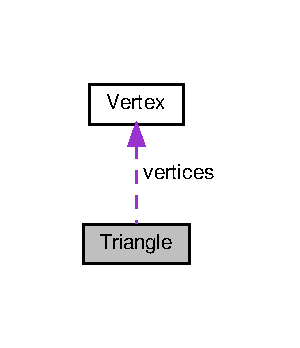
\includegraphics[width=144pt]{class_triangle__coll__graph}
\end{center}
\end{figure}
\subsection*{Public Member Functions}
\begin{DoxyCompactItemize}
\item 
\mbox{\Hypertarget{class_triangle_a420f50ce640dca2aca127ceb68de2e0f}\label{class_triangle_a420f50ce640dca2aca127ceb68de2e0f}} 
{\bfseries Triangle} (\hyperlink{class_vertex}{Vertex} $\ast$vertices, unsigned index)
\item 
\mbox{\Hypertarget{class_triangle_a31d9c90daae516c82e03dcbb492a1fe5}\label{class_triangle_a31d9c90daae516c82e03dcbb492a1fe5}} 
void {\bfseries get\+Vertex} (const unsigned i, Eigen\+::\+Vector3d \&v)
\item 
\mbox{\Hypertarget{class_triangle_ac134db353d4bd34eae298e6220bd0254}\label{class_triangle_ac134db353d4bd34eae298e6220bd0254}} 
void {\bfseries get\+Normal} (Eigen\+::\+Vector3d \&normal)
\item 
\mbox{\Hypertarget{class_triangle_acb81455a547203d7b61b6d178578620a}\label{class_triangle_acb81455a547203d7b61b6d178578620a}} 
void {\bfseries save\+Normal\+And\+Aux\+Info} ()
\item 
\mbox{\Hypertarget{class_triangle_a087e0b0bfb2c49ed4854d8b0e939e7d2}\label{class_triangle_a087e0b0bfb2c49ed4854d8b0e939e7d2}} 
bool {\bfseries ray\+Intersects} (const Eigen\+::\+Vector3d \&ray\+\_\+origin, const Eigen\+::\+Vector3d \&step, double \&t)
\item 
\mbox{\Hypertarget{class_triangle_ac1197111887bcba4098f20a71108105c}\label{class_triangle_ac1197111887bcba4098f20a71108105c}} 
void {\bfseries step\+Intersects\+\_\+\+MT} (\hyperlink{class_walker}{Walker} \&walker, const Eigen\+::\+Vector3d \&step, const double \&max\+\_\+length, \hyperlink{class_collision}{Collision} \&colision)
\item 
\mbox{\Hypertarget{class_triangle_a01e5c101c7455d7030080594628533bf}\label{class_triangle_a01e5c101c7455d7030080594628533bf}} 
void {\bfseries step\+Intersects\+\_\+\+M\+T\+\_\+limits} (const Eigen\+::\+Vector3d \&ray\+\_\+origin, const Eigen\+::\+Vector3d \&step, const double \&max\+\_\+length, \hyperlink{class_collision}{Collision} \&colision, const Eigen\+::\+Vector3d \&limits\+\_\+mod, double limit\+\_\+x, double limit\+\_\+y, double limit\+\_\+z)
\item 
\mbox{\Hypertarget{class_triangle_a733c94320a1effcee36b7382e92be1e6}\label{class_triangle_a733c94320a1effcee36b7382e92be1e6}} 
bool {\bfseries ray\+Intersects\+\_\+\+MT} (const Eigen\+::\+Vector3d \&ray\+\_\+origin, const Eigen\+::\+Vector3d \&step, double \&u, double \&v, double \&t)
\item 
\mbox{\Hypertarget{class_triangle_afd80e0b45910181568098c04e5a2046d}\label{class_triangle_afd80e0b45910181568098c04e5a2046d}} 
double {\bfseries min\+Distance} (const Eigen\+::\+Vector3d p)
\end{DoxyCompactItemize}
\subsection*{Public Attributes}
\begin{DoxyCompactItemize}
\item 
\mbox{\Hypertarget{class_triangle_a0f6509666826b8e916e8c884e6d92fdf}\label{class_triangle_a0f6509666826b8e916e8c884e6d92fdf}} 
unsigned {\bfseries index}
\item 
\mbox{\Hypertarget{class_triangle_a1f17e61561dadac3966d2450dcdb001d}\label{class_triangle_a1f17e61561dadac3966d2450dcdb001d}} 
\hyperlink{class_vertex}{Vertex} $\ast$ {\bfseries vertices}
\item 
\mbox{\Hypertarget{class_triangle_a60f4999d8220f2e9f5361dfc2d3fa7d2}\label{class_triangle_a60f4999d8220f2e9f5361dfc2d3fa7d2}} 
Eigen\+::\+Array3i {\bfseries indexes}
\item 
\mbox{\Hypertarget{class_triangle_a90c44b094ed4f5f663b3198f254b015a}\label{class_triangle_a90c44b094ed4f5f663b3198f254b015a}} 
Eigen\+::\+Vector3d {\bfseries normal}
\item 
\mbox{\Hypertarget{class_triangle_af85e52d2beb9feb49a4ded02061c056a}\label{class_triangle_af85e52d2beb9feb49a4ded02061c056a}} 
Eigen\+::\+Vector3d {\bfseries center}
\item 
\mbox{\Hypertarget{class_triangle_aca1dd750b3a5e13fd86947f318e9176a}\label{class_triangle_aca1dd750b3a5e13fd86947f318e9176a}} 
double {\bfseries radius}
\end{DoxyCompactItemize}


\subsection{Detailed Description}
Auxiliary class. Implements trangular barriers. ===================================/. 

Helper class to strore and handle trangular barriers. \begin{DoxyAuthor}{Author}
Jonathan Rafael 
\end{DoxyAuthor}
\begin{DoxyDate}{Date}
July 2016 \subsection*{0.\+2 }
\end{DoxyDate}


The documentation for this class was generated from the following files\+:\begin{DoxyCompactItemize}
\item 
src/triangle.\+h\item 
src/triangle.\+cpp\end{DoxyCompactItemize}

\hypertarget{class_vertex}{}\section{Vertex Class Reference}
\label{class_vertex}\index{Vertex@{Vertex}}


Auxiliary class. Implements basic vertices. ====================================/.  




{\ttfamily \#include $<$vertex.\+h$>$}

\subsection*{Public Member Functions}
\begin{DoxyCompactItemize}
\item 
\mbox{\Hypertarget{class_vertex_abd9cebad3eacc656ea6a9027c1d96b8d}\label{class_vertex_abd9cebad3eacc656ea6a9027c1d96b8d}} 
{\bfseries Vertex} (const double \&x, const double \&y, const double \&z)
\item 
\mbox{\Hypertarget{class_vertex_a43d933c801f9d4deff63b0ebefa57dd6}\label{class_vertex_a43d933c801f9d4deff63b0ebefa57dd6}} 
double {\bfseries operator()} (unsigned i)
\end{DoxyCompactItemize}
\subsection*{Public Attributes}
\begin{DoxyCompactItemize}
\item 
\mbox{\Hypertarget{class_vertex_a0370aebecc487a440882a2a8b44d0501}\label{class_vertex_a0370aebecc487a440882a2a8b44d0501}} 
unsigned {\bfseries index}
\item 
\mbox{\Hypertarget{class_vertex_a3df67e6d67e5fd518b9ea215722b187f}\label{class_vertex_a3df67e6d67e5fd518b9ea215722b187f}} 
double {\bfseries points} \mbox{[}3\mbox{]}
\end{DoxyCompactItemize}


\subsection{Detailed Description}
Auxiliary class. Implements basic vertices. ====================================/. 

Helper class to strore and handle vertices. \begin{DoxyAuthor}{Author}
Jonathan Rafael 
\end{DoxyAuthor}
\begin{DoxyDate}{Date}
July 2016 \subsection*{0.\+2 }
\end{DoxyDate}


\hyperlink{class_vertex}{Vertex} of a 3d poly 

The documentation for this class was generated from the following files\+:\begin{DoxyCompactItemize}
\item 
src/vertex.\+h\item 
src/vertex.\+cpp\end{DoxyCompactItemize}

\hypertarget{class_voxel}{}\section{Voxel Class Reference}
\label{class_voxel}\index{Voxel@{Voxel}}


//! Main class. Implements basic voxel limits and operations. Class to handle and manage the voxels in the simulations. So far only one voxel at the time can be handled. To improve to several voxels, modifications shall be done.  




{\ttfamily \#include $<$voxel.\+h$>$}



Collaboration diagram for Voxel\+:\nopagebreak
\begin{figure}[H]
\begin{center}
\leavevmode
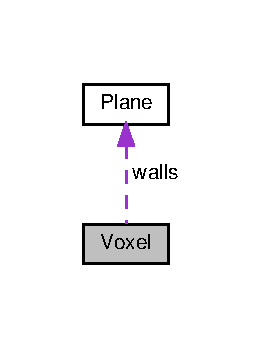
\includegraphics[width=127pt]{class_voxel__coll__graph}
\end{center}
\end{figure}
\subsection*{Public Member Functions}
\begin{DoxyCompactItemize}
\item 
\mbox{\Hypertarget{class_voxel_acbb05a2f277a8ae7c59119eb3adf7e8c}\label{class_voxel_acbb05a2f277a8ae7c59119eb3adf7e8c}} 
{\bfseries Voxel} (Eigen\+::\+Vector3d min\+\_\+limits\+\_\+, Eigen\+::\+Vector3d max\+\_\+limits\+\_\+)
\item 
\mbox{\Hypertarget{class_voxel_af52a1ec58a5244591c56963b28192748}\label{class_voxel_af52a1ec58a5244591c56963b28192748}} 
bool {\bfseries Check\+Collision} (\hyperlink{class_walker}{Walker} \&walker, Eigen\+::\+Vector3d \&step, double \&tmax, \hyperlink{class_collision}{Collision} \&colision)
\end{DoxyCompactItemize}
\subsection*{Public Attributes}
\begin{DoxyCompactItemize}
\item 
\mbox{\Hypertarget{class_voxel_a8f82e23dc4dd9b0a3df065b876525fb4}\label{class_voxel_a8f82e23dc4dd9b0a3df065b876525fb4}} 
Eigen\+::\+Vector3d {\bfseries min\+\_\+limits}
\item 
\mbox{\Hypertarget{class_voxel_a5ffa055c53543ad2dd0944c0667b0787}\label{class_voxel_a5ffa055c53543ad2dd0944c0667b0787}} 
Eigen\+::\+Vector3d {\bfseries max\+\_\+limits}
\item 
\mbox{\Hypertarget{class_voxel_a9cce047be8fe658b21dbaef698b8b5ae}\label{class_voxel_a9cce047be8fe658b21dbaef698b8b5ae}} 
\hyperlink{class_plane}{Plane} {\bfseries walls} \mbox{[}6\mbox{]}
\end{DoxyCompactItemize}


\subsection{Detailed Description}
//! Main class. Implements basic voxel limits and operations. Class to handle and manage the voxels in the simulations. So far only one voxel at the time can be handled. To improve to several voxels, modifications shall be done. 

The documentation for this class was generated from the following files\+:\begin{DoxyCompactItemize}
\item 
src/voxel.\+h\item 
src/voxel.\+cpp\end{DoxyCompactItemize}

\hypertarget{class_walker}{}\section{Walker Class Reference}
\label{class_walker}\index{Walker@{Walker}}


Spin Final class =============================================================/.  




{\ttfamily \#include $<$walker.\+h$>$}



Collaboration diagram for Walker\+:
\nopagebreak
\begin{figure}[H]
\begin{center}
\leavevmode
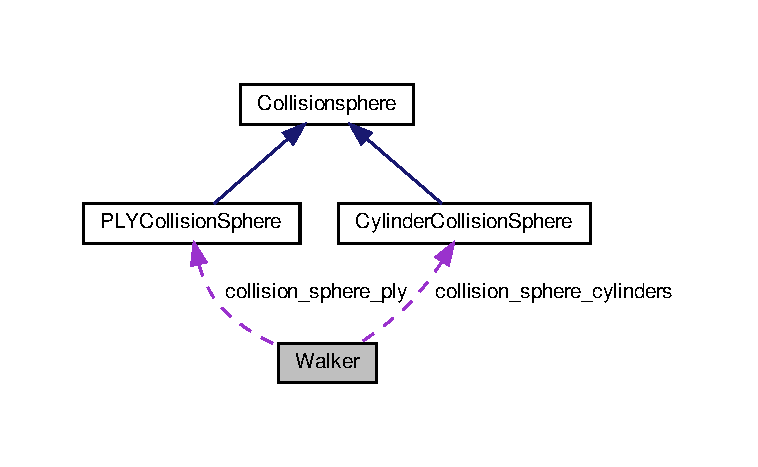
\includegraphics[width=350pt]{class_walker__coll__graph}
\end{center}
\end{figure}
\subsection*{Public Types}
\begin{DoxyCompactItemize}
\item 
enum \hyperlink{class_walker_afcad3f5c11d0bd045de22fb0347dc44c}{state} \{ \newline
{\bfseries on\+\_\+object}, 
{\bfseries on\+\_\+edge}, 
{\bfseries on\+\_\+vertex}, 
{\bfseries on\+\_\+voxel}, 
\newline
{\bfseries free}, 
{\bfseries bouncing}
 \}\begin{DoxyCompactList}\small\item\em An enum. \end{DoxyCompactList}
\item 
enum \hyperlink{class_walker_a24246136a10754791b05cb570dbb8417}{Relative\+Location} \{ {\bfseries unknown}, 
{\bfseries intra}, 
{\bfseries extra}
 \}\begin{DoxyCompactList}\small\item\em An enum. \end{DoxyCompactList}
\end{DoxyCompactItemize}
\subsection*{Public Member Functions}
\begin{DoxyCompactItemize}
\item 
\hyperlink{class_walker_acc0931305bedcf81ff621c31cdf2a92c}{Walker} ()
\begin{DoxyCompactList}\small\item\em Default constructor. \end{DoxyCompactList}\item 
\hyperlink{class_walker_a562c14b600628c18ac689464bd0f7e35}{$\sim$\+Walker} ()
\item 
\hyperlink{class_walker_ada366966172eec6916690c01ac8f01db}{Walker} (double xmin, double xmax, double ymin, double ymax, double zmin, double zmax)
\begin{DoxyCompactList}\small\item\em Constructor. \end{DoxyCompactList}\item 
\mbox{\Hypertarget{class_walker_a682ea5a26950ba7a563ebbf1d1cfe62e}\label{class_walker_a682ea5a26950ba7a563ebbf1d1cfe62e}} 
void {\bfseries get\+Real\+Position} (double \&, double \&, double \&) const
\item 
\mbox{\Hypertarget{class_walker_a85bf9ae51ffcfa9c797ac863bb0ed58a}\label{class_walker_a85bf9ae51ffcfa9c797ac863bb0ed58a}} 
void {\bfseries get\+Real\+Position} (Eigen\+::\+Vector3d \&) const
\item 
\mbox{\Hypertarget{class_walker_a01b46473c4c9126531f86084644be87b}\label{class_walker_a01b46473c4c9126531f86084644be87b}} 
void {\bfseries get\+Voxel\+Position} (double \&, double \&, double \&) const
\item 
\mbox{\Hypertarget{class_walker_aae6ee54e7ca18144ebc63ae30184ac57}\label{class_walker_aae6ee54e7ca18144ebc63ae30184ac57}} 
void {\bfseries get\+Voxel\+Position} (Eigen\+::\+Vector3d \&) const
\item 
\mbox{\Hypertarget{class_walker_a0341476db76d217c0eec89b5f786dc87}\label{class_walker_a0341476db76d217c0eec89b5f786dc87}} 
void {\bfseries get\+Initial\+Position} (double \&, double \&, double \&) const
\item 
\mbox{\Hypertarget{class_walker_a3aa5f7410325a5fc1096684e215e4e3f}\label{class_walker_a3aa5f7410325a5fc1096684e215e4e3f}} 
void {\bfseries get\+Initial\+Position} (Eigen\+::\+Vector3d \&) const
\item 
\mbox{\Hypertarget{class_walker_adf89d9d3c6cd537d2587e51775f9b6ad}\label{class_walker_adf89d9d3c6cd537d2587e51775f9b6ad}} 
void {\bfseries get\+Next\+Direction} (Eigen\+::\+Vector3d \&) const
\item 
\mbox{\Hypertarget{class_walker_a37969cac5ade61c75fb7407b56b535da}\label{class_walker_a37969cac5ade61c75fb7407b56b535da}} 
unsigned int {\bfseries get\+Index} () const
\item 
\mbox{\Hypertarget{class_walker_a47cb165188d588ea04f090648b091654}\label{class_walker_a47cb165188d588ea04f090648b091654}} 
void {\bfseries set\+Real\+Position} (const double \&, const double \&, const double \&)
\item 
\mbox{\Hypertarget{class_walker_ad25cfee48c03072212d9034069002819}\label{class_walker_ad25cfee48c03072212d9034069002819}} 
void {\bfseries set\+Real\+Position} (const Eigen\+::\+Vector3d \&)
\item 
\mbox{\Hypertarget{class_walker_a4d87112b21f490f19e7b942ca94aae20}\label{class_walker_a4d87112b21f490f19e7b942ca94aae20}} 
void {\bfseries set\+Voxel\+Position} (const double \&, const double \&, const double \&)
\item 
\mbox{\Hypertarget{class_walker_aba1f54b57de786fe550ebfcf9f4a7e31}\label{class_walker_aba1f54b57de786fe550ebfcf9f4a7e31}} 
void {\bfseries set\+Voxel\+Position} (const Eigen\+::\+Vector3d \&)
\item 
\mbox{\Hypertarget{class_walker_a06a696a95f7678cb76be214e90e64337}\label{class_walker_a06a696a95f7678cb76be214e90e64337}} 
void {\bfseries set\+Initial\+Position} (const double \&, const double \&, const double \&)
\item 
\mbox{\Hypertarget{class_walker_aafa361803280bc080049ea153867b61d}\label{class_walker_aafa361803280bc080049ea153867b61d}} 
void {\bfseries set\+Initial\+Position} (const Eigen\+::\+Vector3d \&)
\item 
\mbox{\Hypertarget{class_walker_abdeb613b765c45fdabe2891accdbdfb6}\label{class_walker_abdeb613b765c45fdabe2891accdbdfb6}} 
void {\bfseries set\+Next\+Direction} (Eigen\+::\+Vector3d \&)
\item 
\mbox{\Hypertarget{class_walker_aefd71f5bc3303af7e7748bcac5b6ce92}\label{class_walker_aefd71f5bc3303af7e7748bcac5b6ce92}} 
void {\bfseries set\+Random\+Initial\+Position} (const Eigen\+::\+Vector3d \&min, const Eigen\+::\+Vector3d \&max)
\item 
\mbox{\Hypertarget{class_walker_aa6643451a4e13c1d7e121fe710a3bade}\label{class_walker_aa6643451a4e13c1d7e121fe710a3bade}} 
void {\bfseries set\+Index} (unsigned int \&)
\item 
\mbox{\Hypertarget{class_walker_a1fff7bf0f8dde00b9909891f060ac009}\label{class_walker_a1fff7bf0f8dde00b9909891f060ac009}} 
void {\bfseries set\+Real\+Pos\+Log} (const Eigen\+::\+Vector3d \&pos, unsigned t)
\item 
\mbox{\Hypertarget{class_walker_a00a41d2b11cfeffae9ea66f4ea80a568}\label{class_walker_a00a41d2b11cfeffae9ea66f4ea80a568}} 
void {\bfseries set\+Real\+Pos\+Log} (double x, double y, double z, unsigned t)
\item 
\mbox{\Hypertarget{class_walker_adc7b7500ea403ce7dba872ef729c2c40}\label{class_walker_adc7b7500ea403ce7dba872ef729c2c40}} 
void {\bfseries set\+Vox\+Pos\+Log} (const Eigen\+::\+Vector3d \&pos, unsigned t)
\item 
\mbox{\Hypertarget{class_walker_adb197a756c457adc604b6605111e9b92}\label{class_walker_adb197a756c457adc604b6605111e9b92}} 
void {\bfseries set\+Vox\+Pos\+Log} (double x, double y, double z, unsigned t)
\item 
\mbox{\Hypertarget{class_walker_a288f810ee9e4de79a7fe9224de7438b3}\label{class_walker_a288f810ee9e4de79a7fe9224de7438b3}} 
void {\bfseries set\+Number\+Of\+Steps} (unsigned T)
\end{DoxyCompactItemize}
\subsection*{Public Attributes}
\begin{DoxyCompactItemize}
\item 
Eigen\+::\+Vector3d \hyperlink{class_walker_a1008a95833c1f74b53f02e57e84417b7}{pos\+\_\+r}
\item 
Eigen\+::\+Vector3d \hyperlink{class_walker_a2c1bf5a8da9e8f3a230a22ab4ae0e373}{pos\+\_\+v}
\item 
Eigen\+::\+Vector3d \hyperlink{class_walker_a8c78216899e04e9439a991cbad9df36f}{last\+\_\+pos\+\_\+r}
\item 
Eigen\+::\+Vector3d \hyperlink{class_walker_a2d50601346a754183b38890c18e7a6e7}{last\+\_\+pos\+\_\+v}
\item 
Eigen\+::\+Vector3d \hyperlink{class_walker_a98116f0e5d65e1cf65449d80a2d87617}{ini\+\_\+pos}
\item 
Eigen\+::\+Vector3d \hyperlink{class_walker_ad1629485a13c80367a563ed7b88149eb}{next\+\_\+direction}
\item 
Eigen\+::\+Matrix3\+Xd \hyperlink{class_walker_a1ba5a46fddf62eb3eeaabc7c868afe07}{pos\+\_\+r\+\_\+log}
\item 
Eigen\+::\+Matrix3\+Xd \hyperlink{class_walker_a62d99cc92226681123be94e64fb2bf7b}{pos\+\_\+v\+\_\+log}
\item 
int \hyperlink{class_walker_adf221f7a635c09cfaafc0dab5aa38106}{in\+\_\+obj\+\_\+index}
\item 
int \hyperlink{class_walker_a48d0fe08f2297d9ad56cfaec9ee1926c}{in\+\_\+ply\+\_\+index}
\item 
\hyperlink{class_cylinder_collision_sphere}{Cylinder\+Collision\+Sphere} \hyperlink{class_walker_a28d139085430c9a11e0a70be2c3083af}{collision\+\_\+sphere\+\_\+cylinders}
\item 
\hyperlink{class_p_l_y_collision_sphere}{P\+L\+Y\+Collision\+Sphere} \hyperlink{class_walker_a8aecfb76c9007eb6da99b024bc5e425d}{collision\+\_\+sphere\+\_\+ply}
\item 
Eigen\+::\+Vector3d \hyperlink{class_walker_a8a27ead68d3dc7140afbec2710fb3176}{initial\+\_\+sphere\+\_\+pos\+\_\+v}
\item 
unsigned \hyperlink{class_walker_a83536011f160b42f6c39f121ee550731}{steps\+\_\+count}
\item 
\hyperlink{class_walker_afcad3f5c11d0bd045de22fb0347dc44c}{state} \hyperlink{class_walker_afa37629b74387435a0bb02e0c061a718}{status}
\item 
\mbox{\Hypertarget{class_walker_aa80fe894bc14568bdc296083ca5e5492}\label{class_walker_aa80fe894bc14568bdc296083ca5e5492}} 
\hyperlink{class_walker_a24246136a10754791b05cb570dbb8417}{Relative\+Location} {\bfseries initial\+\_\+location}
\item 
\hyperlink{class_walker_a24246136a10754791b05cb570dbb8417}{Relative\+Location} \hyperlink{class_walker_a77f5c801c38158bb8568f75a22baed20}{location}
\item 
int \hyperlink{class_walker_aa211ac1f9a396b1bf3b565e0f8ed098a}{intra\+\_\+extra\+\_\+consensus}
\item 
unsigned \hyperlink{class_walker_a8ca6c90f124e46869ea752920565e2c2}{intra\+\_\+coll\+\_\+count}
\item 
unsigned \hyperlink{class_walker_a28c595f6f6b4c32bed6afb177c0a6608}{extra\+\_\+coll\+\_\+count}
\item 
unsigned int \hyperlink{class_walker_a58e2d14d760748687138b7582cd04365}{index}
\item 
unsigned int \hyperlink{class_walker_a38669698192d39146c77011b69b1e372}{rejection\+\_\+count}
\item 
float \hyperlink{class_walker_a7f33d06b7aa5fabf2a2ac15d119bbcc7}{steps\+\_\+per\+\_\+second}
\end{DoxyCompactItemize}


\subsection{Detailed Description}
Spin Final class =============================================================/. 

Basic unit of the diffusion process.

\begin{DoxyAuthor}{Author}
Jonathan Rafael 
\end{DoxyAuthor}
\begin{DoxyDate}{Date}
November 2016 \subsection*{0.\+2 }
\end{DoxyDate}


Alias for a particle. Basic unit on the simulation process. Saves all the necessary information to perform the particles dynamics. 

\subsection{Member Enumeration Documentation}
\mbox{\Hypertarget{class_walker_a24246136a10754791b05cb570dbb8417}\label{class_walker_a24246136a10754791b05cb570dbb8417}} 
\index{Walker@{Walker}!Relative\+Location@{Relative\+Location}}
\index{Relative\+Location@{Relative\+Location}!Walker@{Walker}}
\subsubsection{\texorpdfstring{Relative\+Location}{RelativeLocation}}
{\footnotesize\ttfamily enum \hyperlink{class_walker_a24246136a10754791b05cb570dbb8417}{Walker\+::\+Relative\+Location}}



An enum. 

Possible location of the walker inside the voxel. Checks illegal crossings of the barrier (border, lol) \mbox{\Hypertarget{class_walker_afcad3f5c11d0bd045de22fb0347dc44c}\label{class_walker_afcad3f5c11d0bd045de22fb0347dc44c}} 
\index{Walker@{Walker}!state@{state}}
\index{state@{state}!Walker@{Walker}}
\subsubsection{\texorpdfstring{state}{state}}
{\footnotesize\ttfamily enum \hyperlink{class_walker_afcad3f5c11d0bd045de22fb0347dc44c}{Walker\+::state}}



An enum. 

All the possibles states that a walker can be in a given step. The next step is perform according to this state 

\subsection{Constructor \& Destructor Documentation}
\mbox{\Hypertarget{class_walker_acc0931305bedcf81ff621c31cdf2a92c}\label{class_walker_acc0931305bedcf81ff621c31cdf2a92c}} 
\index{Walker@{Walker}!Walker@{Walker}}
\index{Walker@{Walker}!Walker@{Walker}}
\subsubsection{\texorpdfstring{Walker()}{Walker()}\hspace{0.1cm}{\footnotesize\ttfamily [1/2]}}
{\footnotesize\ttfamily Walker\+::\+Walker (\begin{DoxyParamCaption}{ }\end{DoxyParamCaption})}



Default constructor. 

Set all variables to cero.

Based class \hyperlink{class_walker}{Walker}. \mbox{\Hypertarget{class_walker_a562c14b600628c18ac689464bd0f7e35}\label{class_walker_a562c14b600628c18ac689464bd0f7e35}} 
\index{Walker@{Walker}!````~Walker@{$\sim$\+Walker}}
\index{````~Walker@{$\sim$\+Walker}!Walker@{Walker}}
\subsubsection{\texorpdfstring{$\sim$\+Walker()}{~Walker()}}
{\footnotesize\ttfamily Walker\+::$\sim$\+Walker (\begin{DoxyParamCaption}{ }\end{DoxyParamCaption})\hspace{0.3cm}{\ttfamily [inline]}}

Default destructor.

Does nothing \mbox{\Hypertarget{class_walker_ada366966172eec6916690c01ac8f01db}\label{class_walker_ada366966172eec6916690c01ac8f01db}} 
\index{Walker@{Walker}!Walker@{Walker}}
\index{Walker@{Walker}!Walker@{Walker}}
\subsubsection{\texorpdfstring{Walker()}{Walker()}\hspace{0.1cm}{\footnotesize\ttfamily [2/2]}}
{\footnotesize\ttfamily Walker\+::\+Walker (\begin{DoxyParamCaption}\item[{double}]{xmin,  }\item[{double}]{xmax,  }\item[{double}]{ymin,  }\item[{double}]{ymax,  }\item[{double}]{zmin,  }\item[{double}]{zmax }\end{DoxyParamCaption})}



Constructor. 

Initialize the walker position in a random position inside the boundaries defined by the limits. 
\begin{DoxyParams}{Parameters}
{\em xmin} & lower x threshold \\
\hline
{\em xmax} & upper x threshold \\
\hline
{\em ymin} & lower y threshold \\
\hline
{\em ymax} & upper y threshold \\
\hline
\end{DoxyParams}


\subsection{Member Data Documentation}
\mbox{\Hypertarget{class_walker_a28d139085430c9a11e0a70be2c3083af}\label{class_walker_a28d139085430c9a11e0a70be2c3083af}} 
\index{Walker@{Walker}!collision\+\_\+sphere\+\_\+cylinders@{collision\+\_\+sphere\+\_\+cylinders}}
\index{collision\+\_\+sphere\+\_\+cylinders@{collision\+\_\+sphere\+\_\+cylinders}!Walker@{Walker}}
\subsubsection{\texorpdfstring{collision\+\_\+sphere\+\_\+cylinders}{collision\_sphere\_cylinders}}
{\footnotesize\ttfamily \hyperlink{class_cylinder_collision_sphere}{Cylinder\+Collision\+Sphere} Walker\+::collision\+\_\+sphere\+\_\+cylinders}

\hyperlink{class_collision}{Collision} sphere for collition against cylidners \mbox{\Hypertarget{class_walker_a8aecfb76c9007eb6da99b024bc5e425d}\label{class_walker_a8aecfb76c9007eb6da99b024bc5e425d}} 
\index{Walker@{Walker}!collision\+\_\+sphere\+\_\+ply@{collision\+\_\+sphere\+\_\+ply}}
\index{collision\+\_\+sphere\+\_\+ply@{collision\+\_\+sphere\+\_\+ply}!Walker@{Walker}}
\subsubsection{\texorpdfstring{collision\+\_\+sphere\+\_\+ply}{collision\_sphere\_ply}}
{\footnotesize\ttfamily \hyperlink{class_p_l_y_collision_sphere}{P\+L\+Y\+Collision\+Sphere} Walker\+::collision\+\_\+sphere\+\_\+ply}

\hyperlink{class_collision}{Collision} sphere for collition against P\+LY meshes \mbox{\Hypertarget{class_walker_a28c595f6f6b4c32bed6afb177c0a6608}\label{class_walker_a28c595f6f6b4c32bed6afb177c0a6608}} 
\index{Walker@{Walker}!extra\+\_\+coll\+\_\+count@{extra\+\_\+coll\+\_\+count}}
\index{extra\+\_\+coll\+\_\+count@{extra\+\_\+coll\+\_\+count}!Walker@{Walker}}
\subsubsection{\texorpdfstring{extra\+\_\+coll\+\_\+count}{extra\_coll\_count}}
{\footnotesize\ttfamily unsigned Walker\+::extra\+\_\+coll\+\_\+count}

counter of collision in the extra-\/side w/r the normal \mbox{\Hypertarget{class_walker_adf221f7a635c09cfaafc0dab5aa38106}\label{class_walker_adf221f7a635c09cfaafc0dab5aa38106}} 
\index{Walker@{Walker}!in\+\_\+obj\+\_\+index@{in\+\_\+obj\+\_\+index}}
\index{in\+\_\+obj\+\_\+index@{in\+\_\+obj\+\_\+index}!Walker@{Walker}}
\subsubsection{\texorpdfstring{in\+\_\+obj\+\_\+index}{in\_obj\_index}}
{\footnotesize\ttfamily int Walker\+::in\+\_\+obj\+\_\+index}

Auxiliar index to save if the walker was inside a convex object \mbox{\Hypertarget{class_walker_a48d0fe08f2297d9ad56cfaec9ee1926c}\label{class_walker_a48d0fe08f2297d9ad56cfaec9ee1926c}} 
\index{Walker@{Walker}!in\+\_\+ply\+\_\+index@{in\+\_\+ply\+\_\+index}}
\index{in\+\_\+ply\+\_\+index@{in\+\_\+ply\+\_\+index}!Walker@{Walker}}
\subsubsection{\texorpdfstring{in\+\_\+ply\+\_\+index}{in\_ply\_index}}
{\footnotesize\ttfamily int Walker\+::in\+\_\+ply\+\_\+index}

Auxiliar index to save if the walker was inside a convex ply object \mbox{\Hypertarget{class_walker_a58e2d14d760748687138b7582cd04365}\label{class_walker_a58e2d14d760748687138b7582cd04365}} 
\index{Walker@{Walker}!index@{index}}
\index{index@{index}!Walker@{Walker}}
\subsubsection{\texorpdfstring{index}{index}}
{\footnotesize\ttfamily unsigned int Walker\+::index}

\hyperlink{class_walker}{Walker} identifier (id) \mbox{\Hypertarget{class_walker_a98116f0e5d65e1cf65449d80a2d87617}\label{class_walker_a98116f0e5d65e1cf65449d80a2d87617}} 
\index{Walker@{Walker}!ini\+\_\+pos@{ini\+\_\+pos}}
\index{ini\+\_\+pos@{ini\+\_\+pos}!Walker@{Walker}}
\subsubsection{\texorpdfstring{ini\+\_\+pos}{ini\_pos}}
{\footnotesize\ttfamily Eigen\+::\+Vector3d Walker\+::ini\+\_\+pos}

\hyperlink{class_walker}{Walker} intital position \mbox{\Hypertarget{class_walker_a8a27ead68d3dc7140afbec2710fb3176}\label{class_walker_a8a27ead68d3dc7140afbec2710fb3176}} 
\index{Walker@{Walker}!initial\+\_\+sphere\+\_\+pos\+\_\+v@{initial\+\_\+sphere\+\_\+pos\+\_\+v}}
\index{initial\+\_\+sphere\+\_\+pos\+\_\+v@{initial\+\_\+sphere\+\_\+pos\+\_\+v}!Walker@{Walker}}
\subsubsection{\texorpdfstring{initial\+\_\+sphere\+\_\+pos\+\_\+v}{initial\_sphere\_pos\_v}}
{\footnotesize\ttfamily Eigen\+::\+Vector3d Walker\+::initial\+\_\+sphere\+\_\+pos\+\_\+v}

Saves the intial positioon of the walker inside the collition sphere \mbox{\Hypertarget{class_walker_a8ca6c90f124e46869ea752920565e2c2}\label{class_walker_a8ca6c90f124e46869ea752920565e2c2}} 
\index{Walker@{Walker}!intra\+\_\+coll\+\_\+count@{intra\+\_\+coll\+\_\+count}}
\index{intra\+\_\+coll\+\_\+count@{intra\+\_\+coll\+\_\+count}!Walker@{Walker}}
\subsubsection{\texorpdfstring{intra\+\_\+coll\+\_\+count}{intra\_coll\_count}}
{\footnotesize\ttfamily unsigned Walker\+::intra\+\_\+coll\+\_\+count}

counter of collision in the ïntra-\/side w/r the normal \mbox{\Hypertarget{class_walker_aa211ac1f9a396b1bf3b565e0f8ed098a}\label{class_walker_aa211ac1f9a396b1bf3b565e0f8ed098a}} 
\index{Walker@{Walker}!intra\+\_\+extra\+\_\+consensus@{intra\+\_\+extra\+\_\+consensus}}
\index{intra\+\_\+extra\+\_\+consensus@{intra\+\_\+extra\+\_\+consensus}!Walker@{Walker}}
\subsubsection{\texorpdfstring{intra\+\_\+extra\+\_\+consensus}{intra\_extra\_consensus}}
{\footnotesize\ttfamily int Walker\+::intra\+\_\+extra\+\_\+consensus}

intra o extra position by face collision consensus w/r the normal \mbox{\Hypertarget{class_walker_a8c78216899e04e9439a991cbad9df36f}\label{class_walker_a8c78216899e04e9439a991cbad9df36f}} 
\index{Walker@{Walker}!last\+\_\+pos\+\_\+r@{last\+\_\+pos\+\_\+r}}
\index{last\+\_\+pos\+\_\+r@{last\+\_\+pos\+\_\+r}!Walker@{Walker}}
\subsubsection{\texorpdfstring{last\+\_\+pos\+\_\+r}{last\_pos\_r}}
{\footnotesize\ttfamily Eigen\+::\+Vector3d Walker\+::last\+\_\+pos\+\_\+r}

\hyperlink{class_walker}{Walker} voxel last position \mbox{\Hypertarget{class_walker_a2d50601346a754183b38890c18e7a6e7}\label{class_walker_a2d50601346a754183b38890c18e7a6e7}} 
\index{Walker@{Walker}!last\+\_\+pos\+\_\+v@{last\+\_\+pos\+\_\+v}}
\index{last\+\_\+pos\+\_\+v@{last\+\_\+pos\+\_\+v}!Walker@{Walker}}
\subsubsection{\texorpdfstring{last\+\_\+pos\+\_\+v}{last\_pos\_v}}
{\footnotesize\ttfamily Eigen\+::\+Vector3d Walker\+::last\+\_\+pos\+\_\+v}

\hyperlink{class_walker}{Walker} real last position \mbox{\Hypertarget{class_walker_a77f5c801c38158bb8568f75a22baed20}\label{class_walker_a77f5c801c38158bb8568f75a22baed20}} 
\index{Walker@{Walker}!location@{location}}
\index{location@{location}!Walker@{Walker}}
\subsubsection{\texorpdfstring{location}{location}}
{\footnotesize\ttfamily \hyperlink{class_walker_a24246136a10754791b05cb570dbb8417}{Relative\+Location} Walker\+::location}

location on the substrate (if known) \mbox{\Hypertarget{class_walker_ad1629485a13c80367a563ed7b88149eb}\label{class_walker_ad1629485a13c80367a563ed7b88149eb}} 
\index{Walker@{Walker}!next\+\_\+direction@{next\+\_\+direction}}
\index{next\+\_\+direction@{next\+\_\+direction}!Walker@{Walker}}
\subsubsection{\texorpdfstring{next\+\_\+direction}{next\_direction}}
{\footnotesize\ttfamily Eigen\+::\+Vector3d Walker\+::next\+\_\+direction}

Auxiliar vector for special states cases, decides the next direction \mbox{\Hypertarget{class_walker_a1008a95833c1f74b53f02e57e84417b7}\label{class_walker_a1008a95833c1f74b53f02e57e84417b7}} 
\index{Walker@{Walker}!pos\+\_\+r@{pos\+\_\+r}}
\index{pos\+\_\+r@{pos\+\_\+r}!Walker@{Walker}}
\subsubsection{\texorpdfstring{pos\+\_\+r}{pos\_r}}
{\footnotesize\ttfamily Eigen\+::\+Vector3d Walker\+::pos\+\_\+r}

Real walker position for collision, r stands for real \mbox{\Hypertarget{class_walker_a1ba5a46fddf62eb3eeaabc7c868afe07}\label{class_walker_a1ba5a46fddf62eb3eeaabc7c868afe07}} 
\index{Walker@{Walker}!pos\+\_\+r\+\_\+log@{pos\+\_\+r\+\_\+log}}
\index{pos\+\_\+r\+\_\+log@{pos\+\_\+r\+\_\+log}!Walker@{Walker}}
\subsubsection{\texorpdfstring{pos\+\_\+r\+\_\+log}{pos\_r\_log}}
{\footnotesize\ttfamily Eigen\+::\+Matrix3\+Xd Walker\+::pos\+\_\+r\+\_\+log}

log of the real spin position, used to compute the phase shift \mbox{\Hypertarget{class_walker_a2c1bf5a8da9e8f3a230a22ab4ae0e373}\label{class_walker_a2c1bf5a8da9e8f3a230a22ab4ae0e373}} 
\index{Walker@{Walker}!pos\+\_\+v@{pos\+\_\+v}}
\index{pos\+\_\+v@{pos\+\_\+v}!Walker@{Walker}}
\subsubsection{\texorpdfstring{pos\+\_\+v}{pos\_v}}
{\footnotesize\ttfamily Eigen\+::\+Vector3d Walker\+::pos\+\_\+v}

\hyperlink{class_walker}{Walker} current position \mbox{\Hypertarget{class_walker_a62d99cc92226681123be94e64fb2bf7b}\label{class_walker_a62d99cc92226681123be94e64fb2bf7b}} 
\index{Walker@{Walker}!pos\+\_\+v\+\_\+log@{pos\+\_\+v\+\_\+log}}
\index{pos\+\_\+v\+\_\+log@{pos\+\_\+v\+\_\+log}!Walker@{Walker}}
\subsubsection{\texorpdfstring{pos\+\_\+v\+\_\+log}{pos\_v\_log}}
{\footnotesize\ttfamily Eigen\+::\+Matrix3\+Xd Walker\+::pos\+\_\+v\+\_\+log}

log of the voxel position, used for collision location and bouncing \mbox{\Hypertarget{class_walker_a38669698192d39146c77011b69b1e372}\label{class_walker_a38669698192d39146c77011b69b1e372}} 
\index{Walker@{Walker}!rejection\+\_\+count@{rejection\+\_\+count}}
\index{rejection\+\_\+count@{rejection\+\_\+count}!Walker@{Walker}}
\subsubsection{\texorpdfstring{rejection\+\_\+count}{rejection\_count}}
{\footnotesize\ttfamily unsigned int Walker\+::rejection\+\_\+count}

counter of the rejected directions in a single time-\/step \mbox{\Hypertarget{class_walker_afa37629b74387435a0bb02e0c061a718}\label{class_walker_afa37629b74387435a0bb02e0c061a718}} 
\index{Walker@{Walker}!status@{status}}
\index{status@{status}!Walker@{Walker}}
\subsubsection{\texorpdfstring{status}{status}}
{\footnotesize\ttfamily \hyperlink{class_walker_afcad3f5c11d0bd045de22fb0347dc44c}{state} Walker\+::status}

state memeber \mbox{\Hypertarget{class_walker_a83536011f160b42f6c39f121ee550731}\label{class_walker_a83536011f160b42f6c39f121ee550731}} 
\index{Walker@{Walker}!steps\+\_\+count@{steps\+\_\+count}}
\index{steps\+\_\+count@{steps\+\_\+count}!Walker@{Walker}}
\subsubsection{\texorpdfstring{steps\+\_\+count}{steps\_count}}
{\footnotesize\ttfamily unsigned Walker\+::steps\+\_\+count}

Counts the number of steps (including bouncings) made. \mbox{\Hypertarget{class_walker_a7f33d06b7aa5fabf2a2ac15d119bbcc7}\label{class_walker_a7f33d06b7aa5fabf2a2ac15d119bbcc7}} 
\index{Walker@{Walker}!steps\+\_\+per\+\_\+second@{steps\+\_\+per\+\_\+second}}
\index{steps\+\_\+per\+\_\+second@{steps\+\_\+per\+\_\+second}!Walker@{Walker}}
\subsubsection{\texorpdfstring{steps\+\_\+per\+\_\+second}{steps\_per\_second}}
{\footnotesize\ttfamily float Walker\+::steps\+\_\+per\+\_\+second}

Particles steps per second speeed. 

The documentation for this class was generated from the following files\+:\begin{DoxyCompactItemize}
\item 
src/walker.\+h\item 
src/walker.\+cpp\end{DoxyCompactItemize}

%--- End generated contents ---

% Index
\backmatter
\newpage
\phantomsection
\clearemptydoublepage
\addcontentsline{toc}{chapter}{Index}
\printindex

\end{document}
